\newcommand*{\ATLASLATEXPATH}{latex/}
%\pdfoutput=1
\documentclass[cernpreprint,texlive=2011,txfonts,UKenglish]{\ATLASLATEXPATH atlasdoc}

\usepackage[full]{\ATLASLATEXPATH atlaspackage}
\usepackage{\ATLASLATEXPATH atlasbiblatex}

\usepackage{\ATLASLATEXPATH atlascontribute}

\usepackage{\ATLASLATEXPATH atlasphysics}
\addbibresource{Paper.bib}
\addbibresource{jpsipipi_JHEP.bib}
\DeclareFieldFormat[phdthesis]{citetitle}{#1}
\DeclareFieldFormat[phdthesis]{title}{#1} 


\graphicspath{{logos/}{figures/}}

 
\usepackage{enumitem}
\usepackage{epstopdf}

\def\ttbar {\mbox {$t\bar{t}$}}
\def\ipb {\mbox {$~{\rm pb}^{-1}$}}
\def\ifb {\mbox {$~{\rm fb}^{-1}$}}
\def\lumiA{\mbox{$2.1\ifb$}}
\def\lumierrA{\mbox{$2.09 \pm 0.04 \ifb$}}
\def\lumiB{\mbox{$11.4\ifb$}}
\def\lumierrB{\mbox{$11.4 \pm 0.3 \ifb$}}
\def\mt{\mbox{$m_{\text{T}}$}}
\def\pt{\mbox{$p_{\text{T}}$}}
\def\et{\mbox{$E_{\text{T}}$}}
\def\kt{\mbox{$k_t$}}
\newcommand{\psiprime}{\ensuremath{\psi(2\mathrm{S})}}
\newcommand{\pjpsi}{prompt \ensuremath{\,\Jpsi}}
\newcommand{\npjpsi}{non-prompt \ensuremath{\,\Jpsi}}
\newcommand{\apsi}{\ensuremath{\psi}}

\hypersetup{pdftitle={Measurement of the differential cross-sections of prompt and non-prompt production of $\jpsi$ and $\psiprime$ in $pp$ collisions at $\sqrt{s} = 7$ and $8$~TeV with the ATLAS detector},pdfauthor={The ATLAS Collaboration}}
%-------------------------------------------------------------------------------
% This file contains the title, author and abstract.
% It also contains all relevant document numbers used by the different cover pages.
%-------------------------------------------------------------------------------

% Title
\AtlasTitle{AtlasTitle: Bare bones ATLAS document}

% Author - this does not work with revtex (add it after \begin{document})
\author{The ATLAS Collaboration}

% Authors and list of contributors to the analysis
% \AtlasAuthorContributor also adds the name to the author list
% Include package latex/atlascontribute to use this
% Use authblk package if there are multiple authors, which is included by latex/atlascontribute
% \usepackage{authblk}
% Use the following 3 lines to have all institutes on one line
% \makeatletter
% \renewcommand\AB@affilsepx{, \protect\Affilfont}
% \makeatother
% \renewcommand\Authands{, } % avoid ``. and'' for last author
% \renewcommand\Affilfont{\itshape\small} % affiliation formatting
% \AtlasAuthorContributor{First AtlasAuthorContributor}{a}{Author's contribution.}
% \AtlasAuthorContributor{Second AtlasAuthorContributor}{b}{Author's contribution.}
% \AtlasAuthorContributor{Third AtlasAuthorContributor}{a}{Author's contribution.}
% \AtlasContributor{Fourth AtlasContributor}{Contribution to the analysis.}
% \author[a]{First Author}
% \author[a]{Second Author}
% \author[b]{Third Author}
% \affil[a]{One Institution}
% \affil[b]{Another Institution}

% If a special author list should be indicated via a link use the following code:
% Include the two lines below if you do not use atlasstyle:
% \usepackage[marginal,hang]{footmisc}
% \setlength{\footnotemargin}{0.5em}
% Use the following lines in all cases:
% \usepackage{authblk}
% \author{The ATLAS Collaboration%
% \thanks{The full author list can be found at:\newline
%   \url{https://atlas.web.cern.ch/Atlas/PUBNOTES/ATL-PHYS-PUB-2014-007/authorlist.pdf}}
% }

% Date: if not given, uses current date
%\date{\today}

% Draft version:
% Should be 1.0 for the first circulation, and 2.0 for the second circulation.
% If given, adds draft version on front page, a 'DRAFT' box on top of each other page, 
% and line numbers.
% Comment or remove in final version.


% ATLAS reference code, to help ATLAS members to locate the paper
\AtlasRefCode{GROUP-2014-XX}

% ATLAS note number. Can be an COM, INT, PUB or CONF note
% \AtlasNote{ATLAS-CONF-2014-XXX}
% \AtlasNote{ATL-PHYS-PUB-2014-XXX}
% \AtlasNote{ATL-COM-PHYS-2014-XXX}

% CERN preprint number
% \PreprintIdNumber{CERN-PH-2014-XX}

% ATLAS date - arXiv submission; to be filled in by the Physics Office
% \AtlasDate{\today}

% arXiv identifier
% \arXivId{14XX.YYYY}

% HepData record
% \HepDataRecord{ZZZZZZZZ}

% Submission journal and final reference
% \AtlasJournal{Phys.\ Lett.\ B.}
% \AtlasJournalRef{\PLB 789 (2014) 123}
% \AtlasDOI{}

% Abstract - % directly after { is important for correct indentation
\AtlasAbstract{%
  This is a bare bones ATLAS document. Put the abstract for the document here.
}

%-------------------------------------------------------------------------------
% The following information is needed for the cover page. The commands are only defined
% if you use the coverpage option in atlasdoc or use the atlascover package
%-------------------------------------------------------------------------------

% List of supporting notes  (leave as null \AtlasCoverSupportingNote{} if you want to skip this option)
% \AtlasCoverSupportingNote{Short title note 1}{https://cds.cern.ch/record/XXXXXXX}
% \AtlasCoverSupportingNote{Short title note 2}{https://cds.cern.ch/record/YYYYYYY}
%
% OR (the 2nd option is deprecated, especially for CONF and PUB notes)
%
% Supporting material TWiki page  (leave as null \AtlasCoverTwikiURL{} if you want to skip this option)
% \AtlasCoverTwikiURL{https://twiki.cern.ch/twiki/bin/view/Atlas/WebHome}

% Comment deadline
% \AtlasCoverCommentsDeadline{DD Month 2014}

% Analysis team members - contact editors should no longer be specified
% as there is a generic email list name for the editors
% \AtlasCoverAnalysisTeam{Peter Analyser, Susan Editor1, Jenny Editor2, Alphonse Physicien}

% Editorial Board Members - indicate the Chair by a (chair) after his/her name
% Give either all members at once (then they appear on one line), or separately
% \AtlasCoverEdBoardMember{EdBoard~Chair~(chair), EB~Member~1, EB~Member~2, EB~Member~3}
% \AtlasCoverEdBoardMember{EdBoard~Chair~(chair)}
% \AtlasCoverEdBoardMember{EB~Member~1}
% \AtlasCoverEdBoardMember{EB~Member~2}
% \AtlasCoverEdBoardMember{EB~Member~3}

% A PUB note has readers and not an EdBoard -- give their names here (one line or several entries)
% \AtlasCoverReaderMember{Reader~1, Reader~2}
% \AtlasCoverReaderMember{Reader~1}
% \AtlasCoverEdBoardMember{Reader~2}

% Editors egroup
% \AtlasCoverEgroupEditors{atlas-GROUP-2014-XX-editors@cern.ch}

% EdBoard egroup
% \AtlasCoverEgroupEdBoard{atlas-GROUP-2014-XX-editorial-board@cern.ch}



\AtlasTitle{Measurement of the differential cross-sections of prompt and non-prompt production of $\jpsi$ and $\psiprime$ in $pp$ collisions at $\sqrt{s} = 7$ and $8$~\TeV\ with the ATLAS detector}
\AtlasNote{ATL-COM-PHYS-2015-161}
\AtlasJournal{Eur.\ Phys.\ J.\ C.}
\PreprintIdNumber{CERN-PH-EP-2015-292}
\AtlasAbstract{The production rates of prompt and non-prompt \jpsi\ and \psiprime\ mesons in their dimuon decay modes are measured using \lumiA\ and \lumiB\ of data collected 
with the ATLAS experiment at the Large Hadron Collider, in proton--proton collisions at
$\sqrt{s}=7$ and $8$~\TeV\ respectively. Production cross-sections for prompt as well as non-prompt sources, ratios of \psiprime\ to \jpsi\ production, 
and the fractions of non-prompt production for \jpsi\ and \psiprime\
are measured as a function of meson transverse momentum and rapidity. 
The measurements are compared to theoretical predictions.}

\begin{document}

\maketitle

\tableofcontents

\clearpage

\section{Introduction}
\label{intro}

Measurements of heavy quark--antiquark bound states (quarkonia) production processes provide 
an insight into the nature of quantum
chromodynamics (QCD) close to the boundary between the perturbative and non-perturbative regimes. 
More than forty years since the discovery of the $\jpsi$, the investigation of
hidden heavy-flavour production in hadronic collisions 
still presents significant challenges to both theory and experiment.

In high-energy hadronic collisions, charmonium states can be produced either directly by 
short-lived QCD sources (``prompt'' production), or by long-lived sources in the decay chains of beauty hadrons (``non-prompt'' production). 
These can be separated experimentally using the
distance between the proton--proton primary interaction and the decay vertex of the quarkonium state.
While {\em Fixed-Order with Next-to-Leading-Log} (FONLL) calculations \cite{FONLL_2001,Cacciari:2012ny}, made within the framework of perturbative QCD, have
been quite successful in describing non-prompt production of various quarkonium states, a satisfactory understanding of the prompt production mechanisms is still to be achieved.


The $\psiprime$ meson is the only vector charmonium state that 
is produced with no significant  contributions from decays of higher-mass quarkonia, 
referred to as feed-down contributions. This
provides a unique opportunity to study production mechanisms specific to
$J^{PC}=1^{--}$ states~\cite{CDFjpsianomaly1,Abulencia:2007us,Abelev:2014qha,Chatrchyan:2011kc,Chatrchyan:2013cla,Aaij:2012ag,Aad:2014fpa,Aaij:2013jxj,Khachatryan:2015rra,Aaij:2013yaa}.
Measurements of the production of $J^{++}$ states with $J=0, 1, 2$,
\cite{CDFjpsianomaly2,ATLAS:2014ala,Chatrchyan:2012ub,Aaij:2013yaa,Aaij:2013dja,LHCb:2012ac},
strongly coupled to the two-gluon channel, allow similar studies in the $CP$-even sector, complementary to the $CP$-odd vector sector. 
Production of $\jpsi$ mesons
\cite{Aad:2011sp,Abulencia:2007us,Aaij:2011jh,Chatrchyan:2011kc,Abelev:2012gx,Chatrchyan:2013cla,Aaij:2013jxj,Abelev:2014qha,CDFjpsianomaly3,CDFjpsianomaly1,D0jpsi1,D0jpsi2,Khachatryan:2015rra,Aad:2014fpa,CDFjpsianomaly2,LHCb:2012af}
arises from a mixture of different sources, receiving contributions from the production of $1^{--}$ and $J^{++}$ states in comparable amounts.


Early attempts to describe the formation of charmonium
\cite{CSM1,CSM2,CSM3,CSM4,CSM5,CSM7,CEM1,CEM2}
using leading-order perturbative QCD 
gave rise to a variety of models, none of which could explain the
large production cross-sections measured at the Tevatron
\cite{CDFjpsianomaly1,CDFjpsianomaly2,CDFjpsianomaly3,D0jpsi1,D0jpsi2}.
Within the colour-singlet model (CSM) \cite{Lansberg:2008gk}, next-to-next-to-leading-order (NNLO) contributions to the hadronic production of S-wave
quarkonia were calculated without introducing any new phenomenological parameters. However,
technical difficulties have so far made it impossible to perform the full NNLO calculation, or to 
extend those calculations to the P-wave states. 
So it is not entirely surprising that the predictions of the model underestimate the experimental data for inclusive production of
\jpsi\ and $\Upsilon$ states, where the feed-down is significant, but offer a better description  for \psiprime\ production \cite{Aad:2011sp,Aad2012dlq}.

Non-relativistic QCD (NRQCD) calculations that include colour-octet (CO) contributions 
\cite{Bodwin:1994jh} introduce a number of phenomenological parameters --- long-distance matrix elements
(LDMEs) --- which are determined from fits to the experimental data, and can hence
describe the cross-sections and differential spectra satisfactorily 
{\cite{CO_LDME1}}. 
However, the attempts to describe the polarization of S-wave quarkonium states using this approach
have not been so successful~\cite{Gong:2012ug},
prompting a suggestion~\cite{Faccioli:2014cqa} that a more coherent approach is needed for the treatment of polarization
within the QCD-motivated models of quarkonium production. 

Neither the CSM nor the NRQCD model gives a satisfactory explanation for the measurement of prompt
\jpsi\ production in association with the $W$~\cite{Aad:2014rua} and $Z$~\cite{Aad:2014kba} bosons: in both cases,
the measured differential cross-section is larger than theoretical expectations~\cite{Li:2010hc,Lansberg:2013wva,Gong:2012ah, Mao:2011kf}.
It is also important to broaden the scope of comparisons 
between theory and experiment by providing a variety of experimental information
about quarkonium production across a wider kinematic range.
In this context, ATLAS has measured the inclusive differential cross-section of \jpsi\  production, with $2.3$~pb$^{-1}$ of integrated luminosity~\cite{Aad:2011sp}, 
at $\sqrt{s} = 7$~\TeV\ using the data collected in 2010, 
as well as the differential cross-sections of the production of  $\chi_c$ states~(4.5~fb$^{-1}$)~\cite{ATLAS:2014ala}, and of the \psiprime\ in its $J/\psi\pi\pi$ decay mode (2.1 fb$^{-1})$~\cite{Aad:2014fpa}, at $\sqrt{s} = 7$~\TeV\ with data collected in 2011.
The cross-section and polarization measurements 
from CDF~\cite{Abulencia:2007us},
CMS~\cite{Chatrchyan:2013cla,Khachatryan:2010yr,CMS},
LHCb~\cite{Aaij:2012ag,Aaij:2013jxj,Aaij:2013yaa,Aaij:2012asz,Aaij:2013nlm,Aaij:2014qea}  
and ALICE~\cite{Abelev:2014qha,Abelev:2011md,Aamodt:2011gj},
cover a considerable variety of charmonium production characteristics in a wide 
kinematic range (transverse momentum $\pt\leq 100$ \GeV\ and rapidities $|y|<5$), thus providing a wealth of
information for a new generation of theoretical models.

This paper presents a precise measurement of
\jpsi\ and  \psiprime\ production in the dimuon decay mode, both at $\sqrt{s} = 7$~TeV
and at $\sqrt{s} = 8$~TeV.
It is presented as a double-differential measurement in transverse momentum and rapidity of the quarkonium state, 
separated into prompt and non-prompt contributions,
covering a range of transverse momenta $8 < \pt\leq 110$ \GeV\ and rapidities $|y|<2.0$. 
The ratios of $\psiprime$ to $\jpsi$  cross-sections for prompt and non-prompt processes are also reported, as well as the 
non-prompt fractions of $\jpsi$ and $\psiprime$.

\section{The ATLAS detector}
\label{sec:atlas}

The ATLAS experiment~\cite{ATLASdetector} is a general-purpose detector consisting of an inner tracker, a calorimeter and a muon spectrometer. 
The inner detector (ID) directly surrounds the interaction point; 
it consists of a silicon pixel detector, a semiconductor tracker and a transition radiation tracker, and is embedded in an axial~$2$ T magnetic field.
The ID covers the pseudorapidity\footnote{ATLAS uses a right-handed coordinate system with its origin at the nominal interaction point (IP) 
in the centre of the detector and the $z$-axis along the beam pipe.
The $x$-axis points from the IP to the centre of the LHC ring, and the $y$-axis points upward. Cylindrical 
coordinates $(r,\phi)$ are used in the transverse plane,
$\phi$ being the azimuthal angle around the beam pipe. The pseudorapidity $\eta$ is defined in terms of the 
polar angle $\theta$ as $\eta=-\ln\tan(\theta/2)$ and the
transverse momentum $p_{\rm T}$ is defined as $p_{\rm T}=p\sin\theta$. The rapidity is defined as 
$y=0.5\ln\left[\left( E + p_z \right)/ \left( E - p_z \right)\right]$,
where $E$ and $p_z$ refer to energy and longitudinal momentum, respectively. The $\eta$--$\phi$ distance 
between two particles is defined as
 $\Delta R=\sqrt{(\Delta\eta)^2 + (\Delta\phi)^2}$.}
range $|\eta| = $ 2.5 and is enclosed by a calorimeter system containing
electromagnetic and hadronic sections.
The calorimeter is surrounded by a large muon spectrometer (MS) in a toroidal magnet system.
The MS consists of monitored drift tubes and cathode strip chambers, designed to provide
precise position measurements in the bending plane in the range $|\eta| <$ 2.7.
Momentum measurements in the muon spectrometer are based on track segments formed in at least two of the three precision chamber planes.

The ATLAS trigger system \cite{ATLAS:trig} is separated into three levels: the hardware-based Level-1 trigger
and the two-stage High Level Trigger (HLT), comprising the Level-2 trigger and Event
Filter, which reduce the 20~MHz proton--proton collision rate to several-hundred Hz of events of interest for data recording to mass storage. 
At Level-1, the muon trigger searches for patterns of hits satisfying different transverse momentum thresholds with a coarse 
position resolution but a fast response time using resistive-plate chambers and thin-gap chambers in the ranges $|\eta| <$ 1.05 and $1.05 <|\eta| < 2.4$, respectively.
Around these Level-1 hit patterns ``Regions-of-Interest'' (RoI) are defined that
serve as seeds for the HLT muon reconstruction. 
The HLT uses dedicated algorithms to incorporate information from both the 
MS and the ID, achieving position and momentum resolution close to that provided by the offline muon reconstruction.





\section{Candidate selection}
\label{sec:data}

The analysis is based on data recorded at the LHC in 2011 and 2012 during proton--proton collisions at centre-of-mass energies of $7$~\TeV\ and $8$~\TeV, respectively.
This data sample corresponds to a total integrated luminosity of \lumiA\ and \lumiB\ for  $7$~\TeV\ data and $8$~\TeV\ data, respectively.

Events were selected  using a trigger requiring two oppositely charged muon candidates, each passing the requirement $\pt>4$~\GeV. 
The muons are constrained to originate from a common vertex, which is fitted with the track parameter uncertainties taken into account. 
The fit is required to satisfy $\chi^2 < 20$ for the one degree of freedom.

For $7$~\TeV\ data, the Level-1 trigger required only spatial coincidences in the MS~\cite{ATLAS:2010kba}. For $8$~\TeV\ data, a $4$~\GeV\ muon $\pt$ threshold was also applied at Level-1, which reduced the trigger efficiency for low-$\pt$ muons.

The offline analysis requires events to have at least two muons, identified by the muon spectrometer and with matching tracks reconstructed in the ID~\cite{muons}.
Due to the ID acceptance, muon reconstruction is possible only for $|\eta| <$ 2.5. 
The selected muons are further restricted to $|\eta| <$ 2.3 to ensure high-quality tracking and triggering, and to reduce the contribution from misidentified muons.
For the momenta of interest in this analysis (corresponding to muons with a transverse momentum of at most $O(100)$ \GeV), measurements of the
muons are degraded by multiple scattering within the MS and so only the ID tracking
information is considered. 
To ensure accurate ID measurements, each muon track must fulfil muon reconstruction and selection requirements~\cite{muons}.
The pairs of muon candidates satisfying these quality criteria are required to have opposite charges.

In order to allow an accurate correction for trigger inefficiencies, each reconstructed muon candidate is required to match a trigger-identified muon
candidate within a cone of $\Delta R = \sqrt{(\Delta\eta)^2 + (\Delta\phi)^2}=0.01$.
Dimuon candidates are obtained from muon pairs, constrained to originate from a common vertex using ID track parameters and uncertainties, with a 
requirement of $\chi^2 < 20$ of the vertex fit for the one degree of freedom.
All dimuon candidates with an invariant mass
within $2.6 < m(\mu\mu) < 4.0$ \GeV\ and within the kinematic range $\pt(\mu\mu) > 8$ \GeV, $|y(\mu\mu)| < 2.0$ are retained for the analysis.
If multiple candidates are found in an event (occurring in approximately $10^{-6}$ of selected events), all candidates are retained.
The properties of the dimuon system, such as invariant mass $m(\mu\mu)$, transverse momentum $\pt(\mu\mu)$, and rapidity $|y(\mu\mu)|$ are determined from the result of the vertex fit.





\section{Methodology}
\label{sec:method}

The measurements are performed in intervals of dimuon $\pt$ and absolute value of the rapidity ($|y|$). 
The term ``prompt'' refers to the $\jpsi$ or $\psiprime$ states --- hereafter called $\apsi$ to refer to either --- are produced 
from short-lived QCD decays, including feed-down from other charmonium states as long as they are also produced
from short-lived sources. If the decay chain producing a $\apsi$ state includes long-lived particles such as
$b$-hadrons, then such $\apsi$ mesons are labelled as ``non-prompt''. Using a simultaneous fit to the invariant mass of the dimuon and its ``pseudo-proper decay time'' 
(described below), prompt and non-prompt signal and background contributions can be extracted from the data.


The probability for the decay of a particle as a function of proper decay time $t$ follows an exponential distribution, 
$p(t) =  1/\tau_{B}\cdot e^{-t/\tau_{B}}$ where $\tau_{B}$ is the mean lifetime of the particle. For each decay, the proper decay time 
can be calculated as $t = L m/p$,
where $L$ is the distance between the particle production and decay vertices, $p$ is the momentum of the particle, and $m$ is its invariant mass.
As the non-prompt decays of $\apsi$ mesons do not fully reconstruct the $b$-hadron decay, the transverse momentum of the 
dimuon system and the reconstructed dimuon invariant mass are used to construct the
``pseudo-proper decay time'', $\tau = L_{xy} m(\mu\mu)/\pt(\mu\mu)$, where $L_{xy} \equiv \vec{L} \cdot \vec{\pt}(\mu\mu)/\pt(\mu\mu)$ 
is the signed projection of the distance of the dimuon decay vertex 
from the primary vertex, $\vec{L}$, onto its transverse momentum, $\vec{\pt}(\mu\mu)$.
This is a good approximation to using the parent $b$-hadron information when the $\psi$ and parent momenta are closely aligned, which is the case for the values of $\psi$
transverse momenta considered here, and  $\tau$
therefore can be used to distinguish statistically between the non-prompt and prompt processes (in which the latter are assumed to decay with vanishingly small lifetime).
If the event contains multiple primary vertices~\cite{ATLASdetector}, the primary vertex closest in $z$ to the dimuon decay vertex is selected.
The effect of selecting an incorrect vertex has been shown~\cite{BJpsiPhi} to have a negligible impact on the extraction of prompt and non-prompt contributions.
If any of the muons in the dimuon candidate contributes to the construction of the primary vertex, the corresponding tracks are removed and the vertex is refitted.


\subsection{Differential cross-section determination}
\label{sec:s:diff_xSecDet}

The differential dimuon prompt and non-prompt production cross-sections times branching ratio 
are measured separately for \jpsi\ and \psiprime\ mesons according to the equations:

\begin{equation}
\frac{\mathrm{d}^2\sigma(pp \rightarrow \psi)}{\mathrm{d}\pt\mathrm{d}y} \times \mathcal{B} (\psi \rightarrow \mu^+\mu^- ) = \frac{N_{\psi}^{\mathrm{p}}}{\Delta \pt \Delta y \times \int\mathcal{L} \mathrm{d}t}
\label{equ:xSecP}
\end{equation}
\begin{equation}
\frac{\mathrm{d}^2\sigma(pp \rightarrow b\bar{b} \rightarrow \psi)}{\mathrm{d}\pt\mathrm{d}y} \times \mathcal{B} (\psi \rightarrow \mu^+\mu^- ) = \frac{N_{\psi}^{\mathrm{np}}}{\Delta \pt \Delta y \times \int\mathcal{L} \mathrm{d}t}
\label{equ:xSecNP}
\end{equation}

\noindent where $\int\mathcal{L} dt$ is the integrated luminosity, $\Delta \pt $ and $ \Delta y$ are the interval sizes in terms of dimuon transverse momentum and
rapidity, respectively, and $N_{\psi}^{\mathrm{p(np)}}$ is the number of observed prompt (non-prompt) $\psi$ mesons in
the slice under study, corrected for acceptance, trigger and reconstruction efficiencies. 
The intervals in $\Delta y$ combine the data from negative and positive rapidities.
These differential cross-sections are determined separately for the \jpsi\ and \psiprime\ states.

The determination of the cross-sections proceeds in several steps. First, a weight is determined for each
selected dimuon candidate equal to the inverse of the total efficiency for each candidate. 
The total weight, $w_\mathrm{tot}$, for each dimuon candidate includes three factors: the fraction of produced $\psi \rightarrow \mu^+\mu^-$ decays with both
muons in the fiducial region $\pt (\mu) > 4$ \GeV\ and $|\eta(\mu)| <$ 2.3 (defined as acceptance, $\mathcal{A}$), the probability that a candidate
within the acceptance satisfies the offline reconstruction selection ($\epsilon_\mathrm{reco}$), and 
the probability that a reconstructed event satisfies the trigger selection 
($\epsilon_\mathrm{trig}$). The weight assigned to a given candidate when calculating the cross-sections is therefore  given by:

\begin{equation*}
w_{\mathrm{tot}}^{-1} = \mathcal{A} \cdot \epsilon_{\mathrm{reco}} \cdot \epsilon_{\mathrm{trig}}.
\end{equation*}

After the weight determination, an unbinned maximum-likelihood fit is performed to these weighted events in each ($\pt (\mu\mu), \ |y(\mu\mu)|$) interval using the 
dimuon invariant mass, $m(\mu\mu)$, and pseudo-proper decay time, $\tau(\mu\mu)$, observables. 
The fitted yields of $\jpsi \rightarrow \mu^+\mu^-$ and $\psiprime \rightarrow \mu^+\mu^-$ are determined separately for prompt and non-prompt processes. 
Finally, the differential cross-section times the  $\psi \rightarrow \mu^+\mu^-$ branching fraction is calculated for each
state by including the integrated luminosity and the $\pt$ and rapidity interval widths as shown in Eqs. (\ref{equ:xSecP}) and (\ref{equ:xSecNP}).


\subsection{Non-prompt fraction}
\label{sec:s:NPFDet}

The non-prompt fraction $f_{b}^{\psi}$ is defined as the number of non-prompt $\psi$ (produced
via the decay of a $b$-hadron) divided by the number of inclusively produced $\psi$ decaying to muon pairs after applying weighting corrections:

\begin{equation*}
f_{b}^{\psi} \equiv \frac{pp \rightarrow b + X \rightarrow \psi + X'}{pp \xrightarrow{\mathrm{Inclusive}} \psi + X'} = \frac{N^{\mathrm{np}}_{\psi}}{N^{\mathrm{np}}_{\psi} + N^{\mathrm{p}}_{\psi}}, 
\end{equation*}

\noindent where this fraction is determined separately for \jpsi\ and \psiprime. 
Determining the fraction from this ratio is advantageous since acceptance and efficiencies largely cancel and the systematic uncertainty is reduced.

\subsection{Ratio of \psiprime\ to \jpsi\ production in prompt and non-prompt production}
\label{sec:s:PNPRatioDet}

The ratio of \psiprime\ to \jpsi\ production, in their dimuon decay modes, is defined as:

\begin{equation*}
R^{\mathrm{p(np)}} =\frac{N^{\mathrm{p(np)}} _{\psi(2\mathrm{S})}}{N^{\mathrm{p(np)}} _{J/\psi}}
\end{equation*}

\noindent where $N_{\psi}^{\mathrm{p(np)}}$ is the number of prompt (non-prompt) \jpsi\ or \psiprime\ mesons decaying into a 
muon pair in an interval of $\pt$ and $y$, corrected for selection efficiencies and acceptance.

For the ratio measurements, similarly to the non-prompt fraction, the acceptance and efficiency corrections 
largely cancel, thus allowing a more precise measurement.
The theoretical uncertainties on such ratios are also smaller, as several dependencies, such as
parton distribution functions and $b$-hadron production spectra, largely cancel in the ratio.

\subsection{Acceptance}

The kinematic acceptance $\mathcal{A}$ for a $\psi \rightarrow \mu^+\mu^-$ decay with $\pt$ and $y$ is given by the 
probability that both muons pass the fiducial selection ($\pt(\mu)>4$ \GeV\ and $|\eta(\mu)|<2.3$).
This is calculated using generator-level simulations. 
Detector-level corrections, which are found to be small, are applied to the 
results and also considered as part of the systematic uncertainties. 

The acceptance $\mathcal{A}$ depends on five independent variables (the two muon momenta are constrained by the
$m(\mu\mu)$ mass condition), chosen as the $\pt$, $|y|$ and azimuthal angle $\phi$ of the $\psi$ meson in the laboratory frame,
and two angles
characterizing the $\psi \rightarrow \mu^+\mu^-$ decay, $\theta^{\star}$ and $\phi^{\star}$, described in detail in Ref. \cite{Faccioli:2010kd}.
The angle $\theta^{\star}$ is the angle between the direction of the positive-muon momentum in the $\psi$ rest frame
and the momentum of the $\psi$ in the laboratory frame, while $\phi^{\star}$ is defined as the angle between the dimuon 
production and decay planes in the laboratory frame. 
The $\psi$ production plane is defined by the momentum of the $\psi$ in the laboratory frame and the positive $z$-axis direction.
The distributions in $\theta^{\star}$ and $\phi^{\star}$ 
differ for various possible spin-alignment scenarios of the dimuon system.

The spin-alignment of the $\psi$ may vary depending on the production mechanism, which in turn affects the angular distribution of the dimuon decay.
Predictions of various theoretical models are quite contradictory, while the recent experimental measurements~\cite{Chatrchyan:2013cla} indicate that the angular dependence of $\jpsi$ and $\psiprime$
decays is consistent with being isotropic.  

The coefficients $\lambda_{\theta}, \lambda_{\phi}, \lambda_{\theta\phi}$ in
\begin{equation*}
\frac{\mathrm{d}^2N}{\mathrm{d}\cos\theta^{\star}\mathrm{d}\phi^{\star}} \propto 1 + \lambda_{\theta} \cos^2\theta^{\star} + \lambda_{\phi} \sin^2\theta^{\star}\cos2\phi^{\star} +  \lambda_{\theta\phi} \sin2\theta^{\star}\cos\phi^{\star}
\label{equ:acc}
\end{equation*}
\noindent are related to the spin-density matrix elements of the dimuon spin wave function. 

Since the polarization of the $\psi$ state may affect acceptance, seven extreme cases that lead to the largest possible variations of 
acceptance within the phase space of this measurement are identified.
These cases, described in Table~\ref{tab:spin}, are used to define a range in which the results may vary under any physically allowed spin-alignment assumptions.
The same technique has also been used in other measurements~\cite{Aad:2014fpa,ATLAS:2014ala,Aad2012dlq}.
This analysis adopts the isotropic distribution in both $\cos\theta^{\star}$ and $\phi^{\star}$ as  nominal,
and the variation of the results for a  number of extreme spin-alignment scenarios is studied and presented as sets of correction factors,
 detailed further in Appendix~\ref{sec:spincorrection}.
 
\begin{table}[htbp]
\begin{center}
\caption{Values of angular coefficients describing the considered spin-alignment scenarios.}
\vspace{2mm}
\begin{tabular}[h]{r|ccc}
\hline\hline
      & \multicolumn{3}{c}{Angular coefficients} \\ 
      & $\lambda_{\theta}$ & $\lambda_{\phi}$ & $\lambda_{\theta\phi}$ \\ \hline
Isotropic {\em (central value)}            & $0$ & $0$ & $0$ \\
Longitudinal         & $-1$ & $0$ & $0$ \\
Transverse positive  & $+1$ & $+1$ & $0$ \\
Transverse zero      & $+1$                & $0$ & $0$ \\
Transverse negative  & $+1$            & $-1$ & $0$ \\
Off-($\lambda_{\theta}$--$\lambda_{\phi}$)-plane positive   & $0$ & $0$ & $+0.5$ \\
Off-($\lambda_{\theta}$--$\lambda_{\phi}$)-plane negative   & $0$ & $0$ & $-0.5$ \\
\hline\hline
\end{tabular}
\label{tab:spin}
\end{center}
\end{table}


 
For each of the two mass-points (corresponding to the \jpsi\ and \psiprime\ masses), two-dimensional maps are produced
as a function of dimuon $\pt(\mu\mu)$ and $|y(\mu\mu)|$ for the set of spin-alignment hypotheses. 
Acceptance maps are defined within the range $8 < \pt(\mu\mu) < 110$ \GeV, $|y(\mu\mu)| < 2.0$, corresponding to the data
considered in the analysis. 
The map is defined by 100 slices in $|y(\mu\mu)|$ and 4400 in $\pt(\mu\mu)$, using 200k trials for each point, resulting in sufficiently high precision that the statistical uncertainty can be neglected.
Due to the contributions of background, and the detector resolution of the signal the acceptance for each candidate is determined from a linear interpolation of the two maps, which are generated for the \jpsi\ and \psiprime\ known masses, as a function of the reconstructed mass $m(\mu\mu)$.

Figure~\ref{fig:accMapUnpolBoth} shows the acceptance, projected in $\pt$ for all the spin-alignment hypotheses for the \jpsi\ meson.
The differences between the acceptance of the $\psiprime$ and $\jpsi$ meson, are independent of rapidity, except near $|y|\approx2$
at low $\pt$. Similarly, the only dependence on $\pt$ is found below $\pt\approx9$~\GeV.

\begin{figure}[ht]
  \begin{center}
    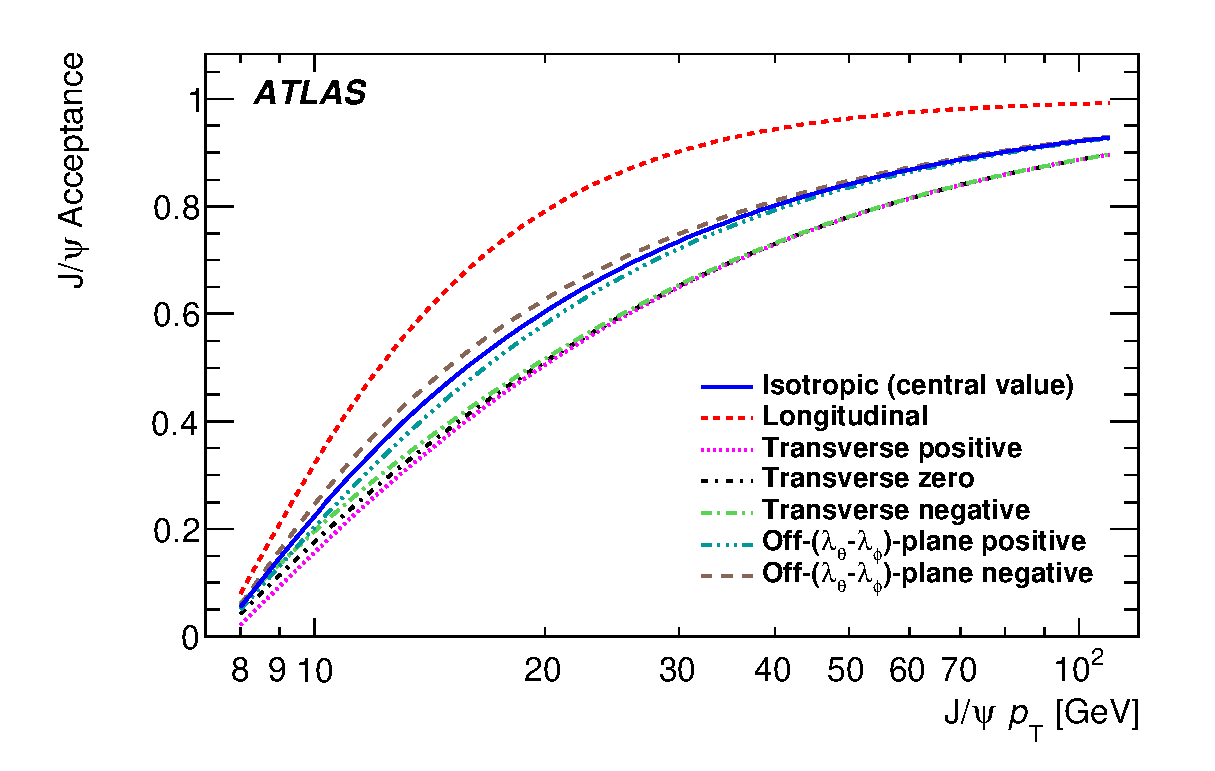
\includegraphics[width=0.8\textwidth]{c_JpsiAcc_All1D_logx.eps}
     \caption{Projections of the acceptance as a function of $\pt$ for the \jpsi\ meson for various spin-alignment hypotheses.}
     \label{fig:accMapUnpolBoth}
  \end{center}
\end{figure}



\subsection{Muon reconstruction and trigger efficiency determination}

\noindent The technique for correcting the 7~\TeV\ data for trigger and reconstruction inefficiencies is described in detail in Ref.~\cite{Aad:2014fpa,Aad2012dlq}.
For the 8~\TeV\ data, a similar technique is used, however different efficiency maps are required for each set of data, and the 8~\TeV\ corrections are detailed briefly below.

The single-muon reconstruction efficiency is determined from a tag-and-probe study in dimuon decays~\cite{Aad:2014kba}.
The efficiency map is calculated as a function of $\pt (\mu)$ and  $q\times \eta(\mu)$, where $q=\pm1$ is the electrical charge of the muon, expressed in units of $e$.

The trigger efficiency correction consists of two components. The first part represents the trigger efficiency for a 
single muon in intervals of $\pt (\mu)$ and $q\times \eta(\mu)$.
For the dimuon system there is a second correction to account for reductions in efficiency due to closely spaced
muons firing only a single RoI, 
vertex-quality cuts, and opposite-sign requirements.
This correction is performed in three rapidity intervals: 0--1.0, 1.0--1.2 and 1.2--2.3. The correction is a function of $\Delta R(\mu\mu)$ 
in the first two rapidity intervals and a function of $\Delta R(\mu\mu)$ and $|y(\mu\mu)|$ in the last interval.

The combination of the two components (single-muon efficiency map and dimuon corrections) is illustrated 
in Figure~\ref{fig:EFmu4DataJpsiTandPCmumupolyL2StarBMaxpt50} by plotting the average trigger-weight correction for the events in this analysis
in terms of $\pt(\mu\mu)$ and $|y(\mu\mu)|$.
The increased weight at low $\pt$ and $|y|\approx 1.25$ is caused by the geometrical acceptance of the muon trigger system and the turn-on threshold behaviour of the muon trigger. At high $\pt$ the weight is increased due to the reduced opening angle between the two muons.


\begin{figure} [!ht]
   \begin{center}
    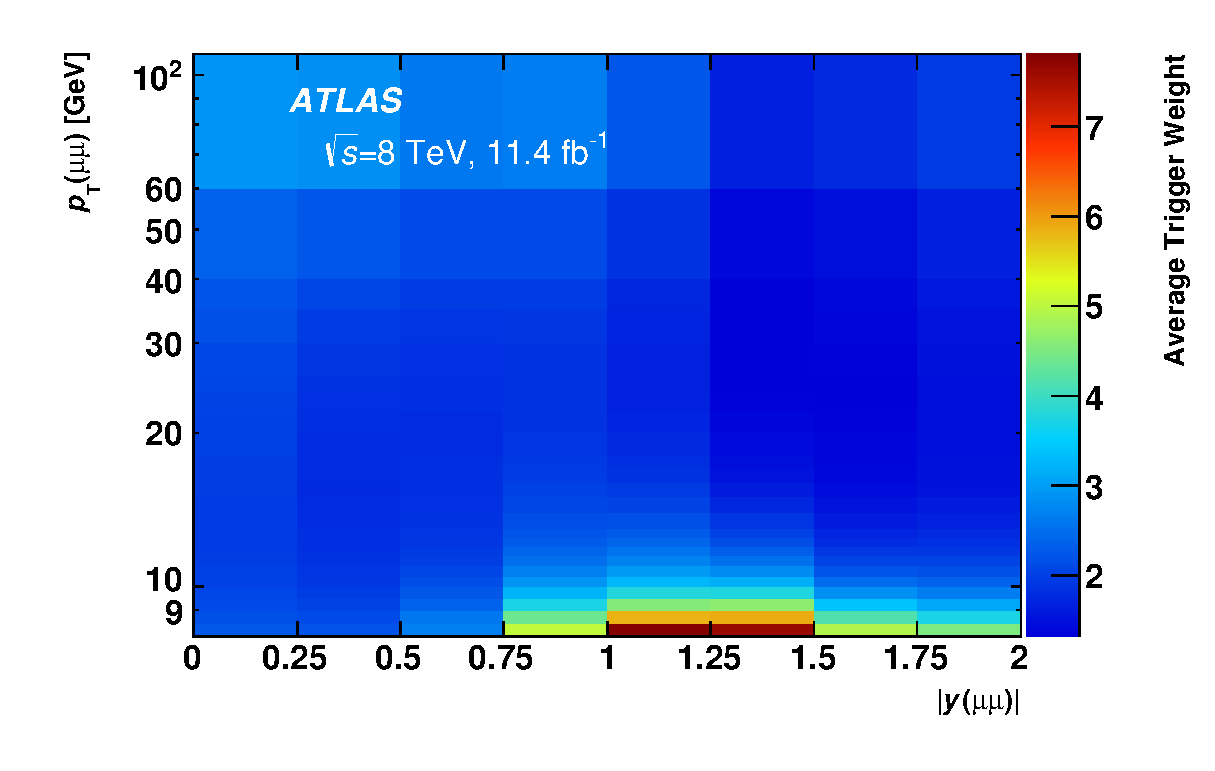
\includegraphics[scale=0.6]{averageTrigWeightMean.eps}
    \caption{Average dimuon trigger-weight in the intervals of $\pt (\mu\mu) $ and $ |y(\mu\mu)|$ studied in this set of measurements. 
    }
    \label{fig:EFmu4DataJpsiTandPCmumupolyL2StarBMaxpt50}
   \end{center}
\end{figure}


\subsection{Fitting technique}
\label{sec:method:fit}

The corrected prompt and non-prompt \jpsi\ and \psiprime\ signal yields are extracted from two-dimensional
weighted unbinned maximum-likelihood fits performed on the dimuon invariant mass ($m(\mu\mu)$)
and pseudo-proper decay time ($\tau(\mu\mu)$) in $(\pt (\mu\mu),|y(\mu\mu)|)$ intervals.
Each interval is fitted independently from all the others.
The probability density function (PDF) for each fit is defined as a normalized sum, 
where each term represents a specific signal or background contribution, with a physically motivated mass and $\tau$ dependence.
The PDF can be written in a compact form as
\begin{equation}
\label{eqn:pdf}
\mathrm{PDF}(m,\tau) = \sum_{i=1}^{7} \kappa_i f_i(m) \ \cdot h_i(\tau) \otimes R(\tau),
\end{equation}
where $\kappa_i$ represents the relative normalization of the $i^\mathrm{th}$ term of the seven considered signal and background contributions (such that $\sum_i \kappa_i = 1$), 
$f_i(m)$ is the mass-dependent term, and $\otimes$ represents the convolution of 
the $\tau$-dependent function $h_i(\tau)$ with the $\tau$ resolution term, $R(\tau)$. 
The latter is modelled by a double Gaussian distribution with both means fixed to zero and widths determined from the fit.

Table \ref{table:fitModel} lists the contributions to the overall PDF with the corresponding $f_i$ and
$h_i$ functions. Here $G_1$ and $G_2$ are Gaussian functions, $B_1$ and $B_2$ are Crystal Ball\footnote{The Crystal Ball function is given by:
\\$B(x;\alpha,n,\bar x,\sigma) = N \cdot \begin{cases} \exp\left(- \frac{(x - \bar x)^2}{2 \sigma^2}\right), & \mbox{for }\frac{x - \bar x}{\sigma} > -\alpha \\
 A \cdot \left(A' - \frac{x - \bar x}{\sigma}\right)^{-n}, & \mbox{for }\frac{x - \bar x}{\sigma} \leqslant -\alpha \end{cases}$ \\where $A = \left(\frac{n}{\left| \alpha \right|}\right)^n \cdot \exp\left(- \frac {\left| \alpha \right|^2}{2}\right),
A' = \frac{n}{\left| \alpha \right|}  - \left| \alpha \right|$}
distributions~\cite{CB1}, 
while F is a uniform distribution and $C_1$ a first-order Chebyshev polynomial. 
The exponential functions $E_1$, $E_2$, $E_3$, $E_4$ and $E_5$
have different decay constants, where $E_5(|\tau|)$ is a double-sided exponential with the same decay constant on
either side of $\tau = 0$. The parameter $\omega$ represents the fractional contribution 
of the $B$ and $G$ mass signal functions, while $\delta (\tau)$, the Dirac delta function,  
is used to represent the pseudo-proper decay time distribution of the prompt candidates.

\begin{table}[h!]
  \centering
  \caption{Description of the fit model PDF in Eq.~\ref{eqn:pdf}. Components of the probability density function used to extract the prompt (P) and
non-prompt (NP) contributions for \jpsi\ and \psiprime\ signal and the P, NP, and incoherent or mis-reconstructed  background (Bkg) contributions.}
    \begin{tabular}{ l  c  c  c  c  }
      \hline \hline
      $i$ & Type & Source & $f_i(m)$ & $h_i(\tau)$ \\ \hline \hline
      1 & \jpsi\     & P     & $\omega B_1(m) + (1-\omega) G_1(m)$   & $\delta (\tau)$ \\
      2 & \jpsi\     & NP    & $\omega B_1(m) + (1-\omega) G_1(m)$   & $ E_1(\tau)$ \\
      3 & \psiprime\    & P    & $\omega B_2(m) + (1-\omega) G_2(m)$   & $\delta (\tau)$ \\
      4 & \psiprime\   & NP    & $\omega B_2(m) + (1-\omega) G_2(m)$   & $E_2(\tau)$ \\ \hline
      5 & Bkg          & P     & $ F$     & $\delta (\tau)$ \\
      6 & Bkg          & NP    & $ C_1(m)$    & $E_3 (\tau)$ \\ 
      7 & Bkg          & NP    & $ E_4(m)$   & $E_5 (|\tau|)$ \\
      \hline  
    \end{tabular}
  \label{table:fitModel}
\end{table}

In order to make the fitting procedure more robust and to reduce the number of free parameters, a number of component terms share common parameters, 
which led to 22 free parameters per interval.
In detail, the signal mass models are described by the sum of a Crystal Ball shape ($B$) and a Gaussian shape ($G$). For each
of \jpsi\ and \psiprime, the $B$ and $G$ share a common mean, and freely determined widths, 
with the ratio of the $B$ and $G$ widths common to \jpsi\ and \psiprime.
The $B$ parameters $\alpha$, and $n$, describing the transition point of the low-edge from a Gaussian to a power-law 
shape, and the shape of the tail, respectively, are fixed, and variations are considered as part of the fit model
systematic uncertainties.
The width of $G$ for \psiprime\ is set to the width for \jpsi\ multiplied by a free parameter scaling term.
The relative fraction of $B$ and $G$ is left floating, but common to \jpsi\ and \psiprime.

The non-prompt signal decay shapes ($E_1$,$E_2$) are described by an exponential function (for positive $\tau$ only) convolved with a
double Gaussian function, $R(\tau)$ describing the pseudo-proper decay time resolution for the non-prompt component, 
and the same Gaussian response functions to
describe the prompt contributions. 
Each Gaussian resolution component has its mean fixed at $\tau$ = 0 and a free width.
The decay constants of the \jpsi\ and \psiprime\ are separate free parameters in the fit.

The background contributions are described by a prompt and non-prompt component, as well as a double-sided exponential function
convolved with a double Gaussian function describing mis-reconstructed or non-coherent dimuon pairs. 
The same resolution function as in signal is used to describe the background. For the non-resonant mass
parameterizations, the non-prompt contribution is modelled by a first-order Chebyshev polynomial. The prompt mass
contribution follows a flat distribution and the double-sided background uses an exponential function.
Variations of this fit model are considered as systematic uncertainties.

The following quantities are extracted directly from the fit in each interval:
the fraction of events that are signal (prompt or non-prompt \jpsi\ or \psiprime); the fraction of signal events that are prompt;
the fraction of prompt signal that is \psiprime; and the fraction of non-prompt signal that is \psiprime. From these
parameters, and the weighted sum of events, all measured values are calculated.


For $7$~\TeV\ data, 168 fits are performed across the range of $8<\pt<100$~\GeV\ ($8<\pt<60$~\GeV) for $\jpsi$ ($\psiprime$) and $0<|y|<2$.
For $8$~\TeV\ data, 172 fits are performed across the range of $8<\pt<110$~\GeV\ and $0<|y|<2$,
excluding the area where $\pt$ is less than 10 \GeV\ and simultaneously $|y|$ is
greater than 0.75. This region is excluded due to a steeply changing low trigger efficiency 
causing large systematic uncertainties in the measured cross-section.

Figure~\ref{fig:fitprojmain} shows the fit results for one of the intervals considered in the analysis with the overall and individual contributions superimposed on the data, and projected onto the invariant mass and pseudo-proper decay time distributions for  $7$~\TeV\ data.
In Figure~\ref{fig:fitprojmainVIII} the fit results are shown for one high-$\pt$ interval of $8$~\TeV\  data.

\begin{figure} [!ht]
  \begin{center} 
   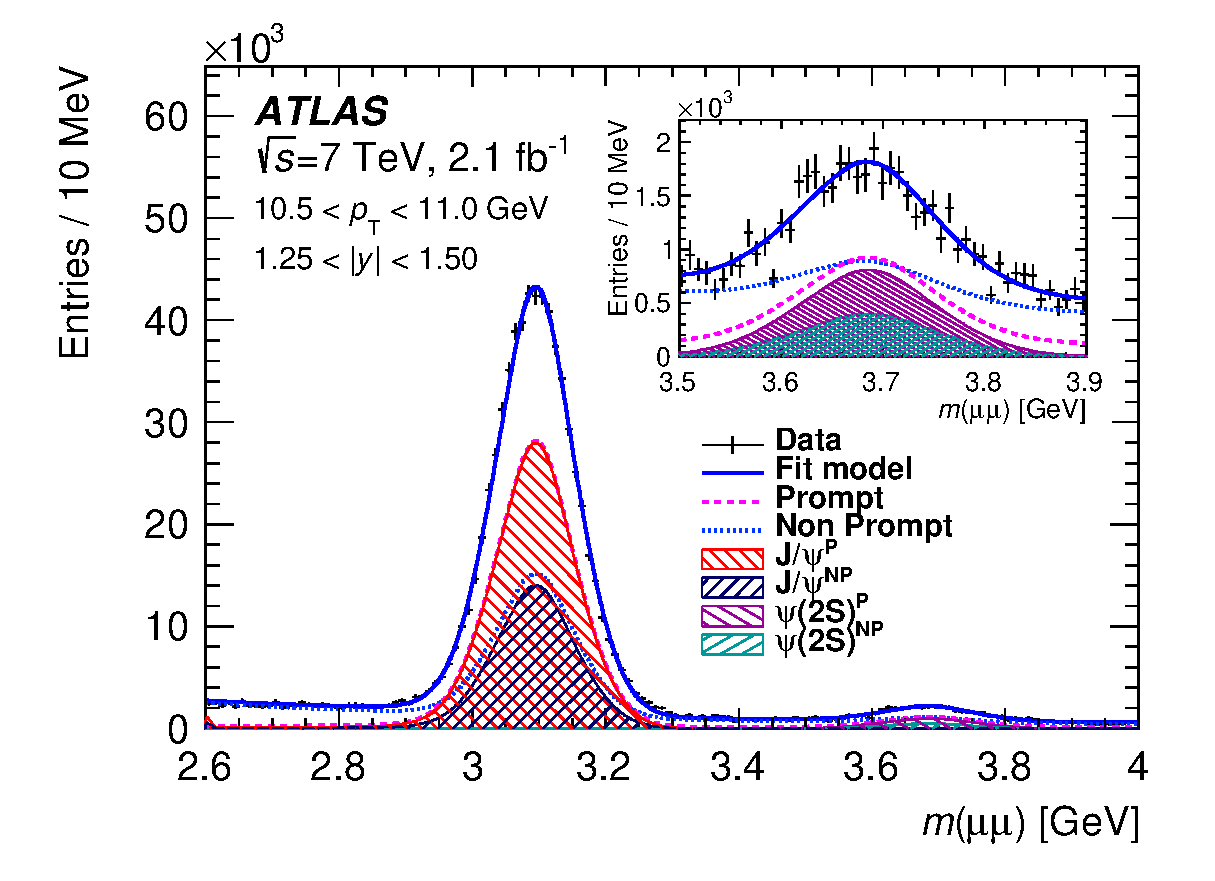
\includegraphics[width=0.51\textwidth]{figures/c_c_Mass_5_5.eps}
   \hspace{-0.55cm}
   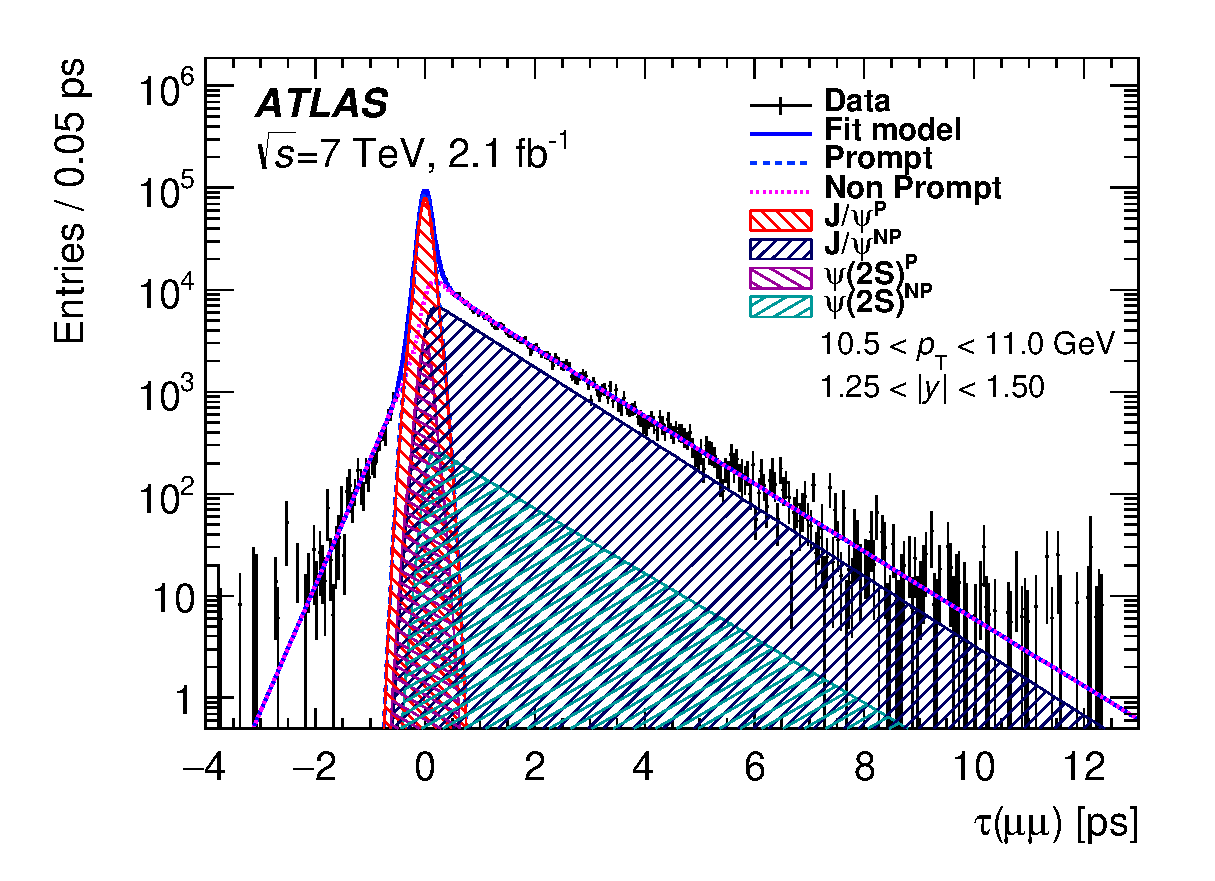
\includegraphics[width=0.51\textwidth]{figures/c_c_Tau_5_5.eps}
      \caption{Projections of the fit result over the mass (left) and pseudo-proper decay time (right) distributions for data collected at $7$~\TeV\  for one typical interval. The data are shown with error bars in black, superimposed with the individual components of the fit result projections, where the total prompt and non-prompt components are represented by the dashed and dotted lines, respectively, and the shaded areas show the signal $\psi$ prompt and non-prompt contributions.\label{fig:fitprojmain}}
  \end{center}
\end{figure} 

\begin{figure} [!ht]
  \begin{center} 
   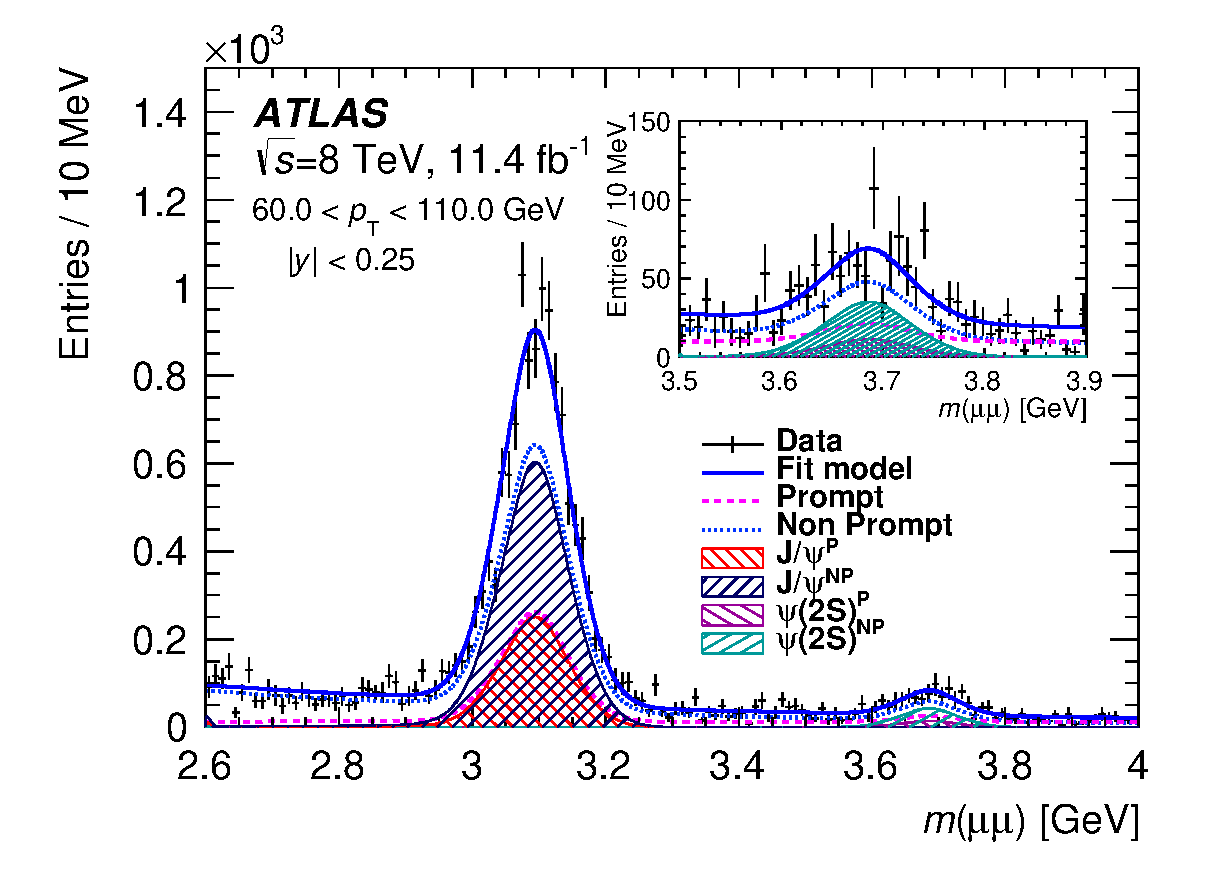
\includegraphics[width=0.51\textwidth]{figures/c_8TeV_c_Mass_23_0.eps}
   \hspace{-0.55cm}
   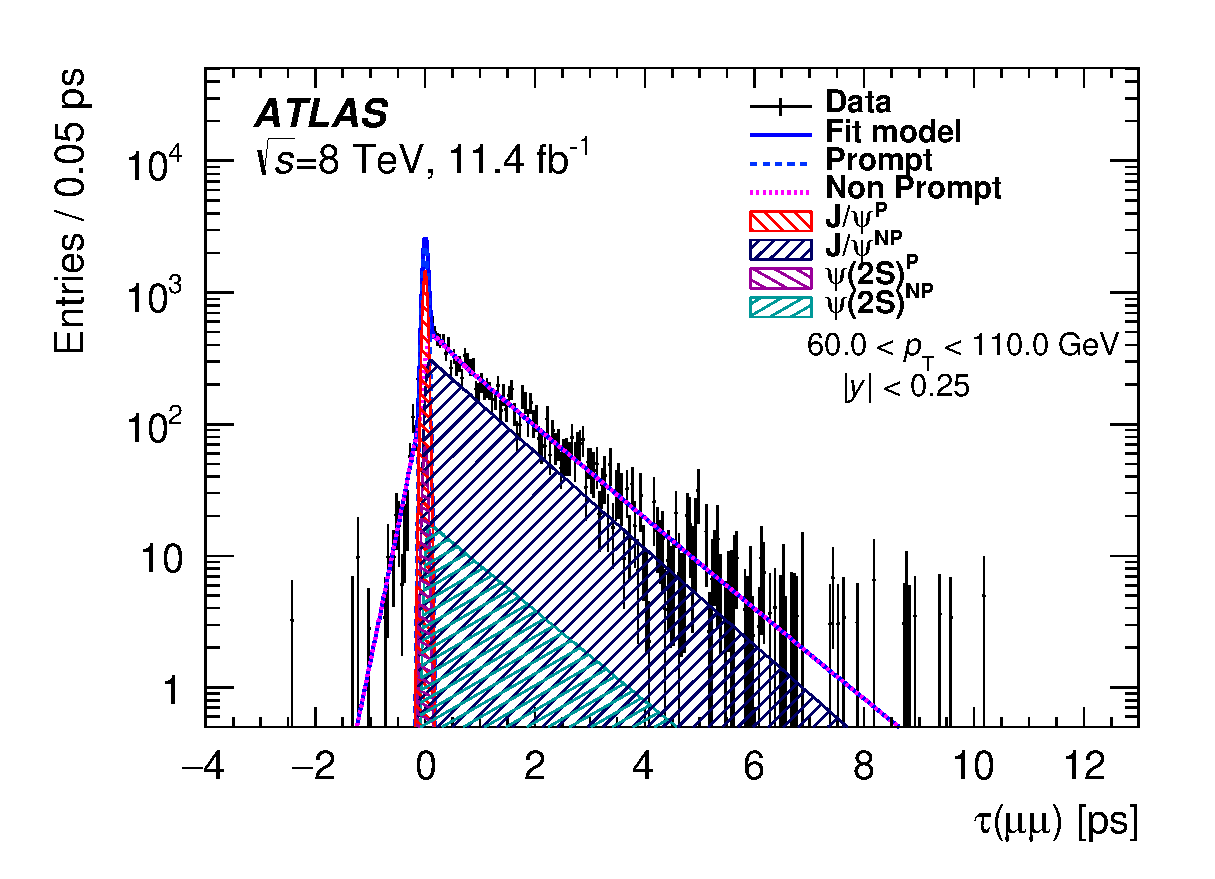
\includegraphics[width=0.51\textwidth]{figures/c_8TeV_c_Tau_23_0.eps}
      \caption{Projections of the fit result over the mass (left) and pseudo-proper decay time (right) distributions for data collected at $8$~\TeV\ for one high-$\pt$ interval. The data are shown with error bars in black, superimposed with the individual components of the fit result projections, where the total prompt and non-prompt components are represented by the dashed and dotted lines, respectively, and the shaded areas show the signal $\psi$ prompt and non-prompt contributions.\label{fig:fitprojmainVIII}}
  \end{center}
\end{figure} 


\subsection{Bin migration corrections}

To account for bin migration effects due to the detector resolution, corrections are applied according to the $\pt$ of the dimuon system.
These corrections are derived from data by comparing analytic functions that are 
fitted to the $\pt$ spectra of dimuon events with and without
convolution by the experimental resolution in $\pt$ (as determined from the fitted mass resolution and measured muon angular resolutions), 
as described in Ref.~\cite{Aad2012dlq}.

The numbers of acceptance- and efficiency-corrected dimuon decays extracted from
the fits in each $\pT$ and rapidity interval are corrected for the differences
between the true and reconstructed values of the dimuon $\pt$.
The correction factors applied to the fitted yields deviate from unity by no more than $1.5\%$, and for the majority of slices are smaller than $1\%$.
The ratio measurement and non-prompt fractions are corrected by the corresponding ratios of
bin migration correction factors.
Using a similar technique, bin migration corrections as a function of $|y|$ are found 
to differ from unity by negligible amounts.



\section{Systematic uncertainties}
\label{sec:syst}

\begin{figure} [!h]
  \begin{center}
    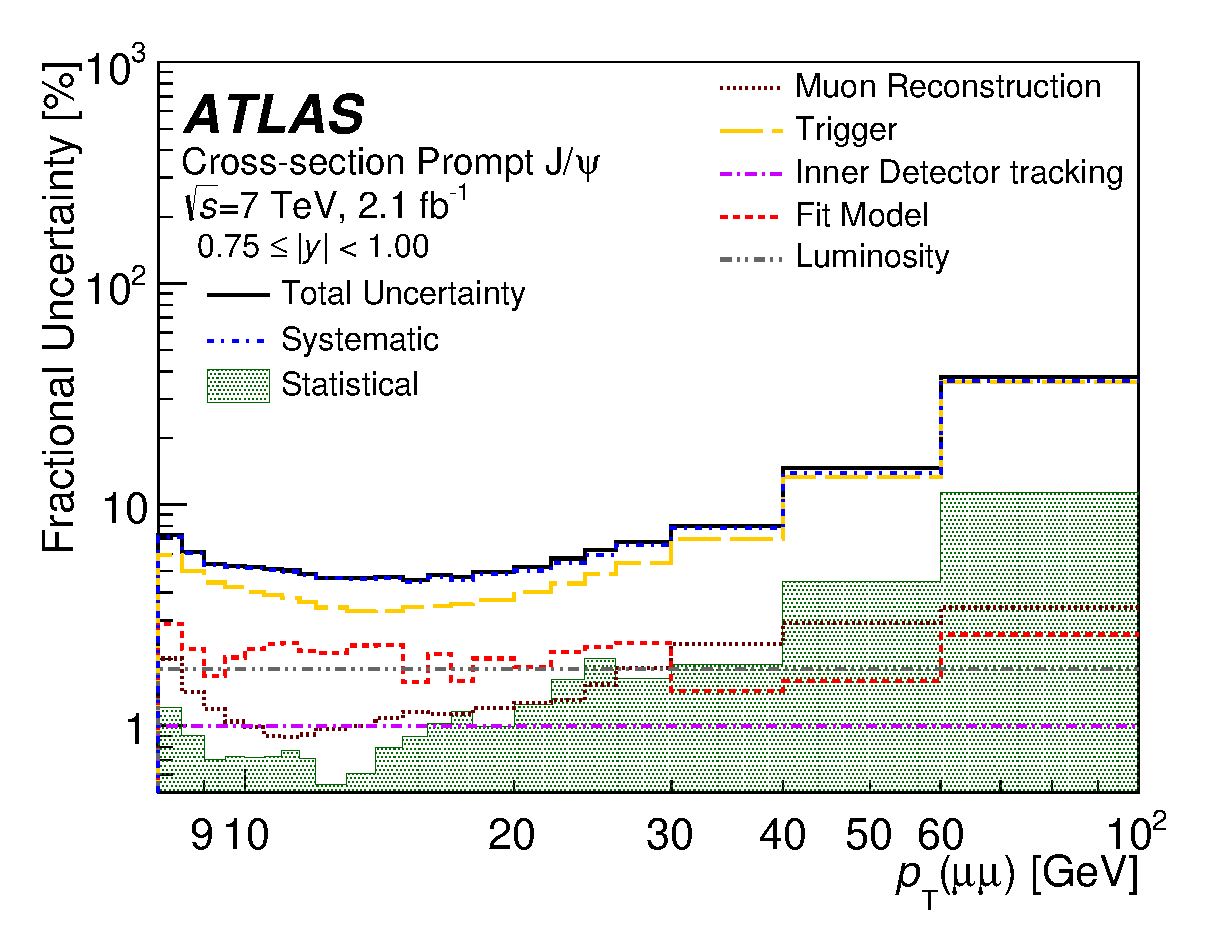
\includegraphics[width=0.49\textwidth]{hs_all_rap_0p75_1p00_jpsiP.eps}
    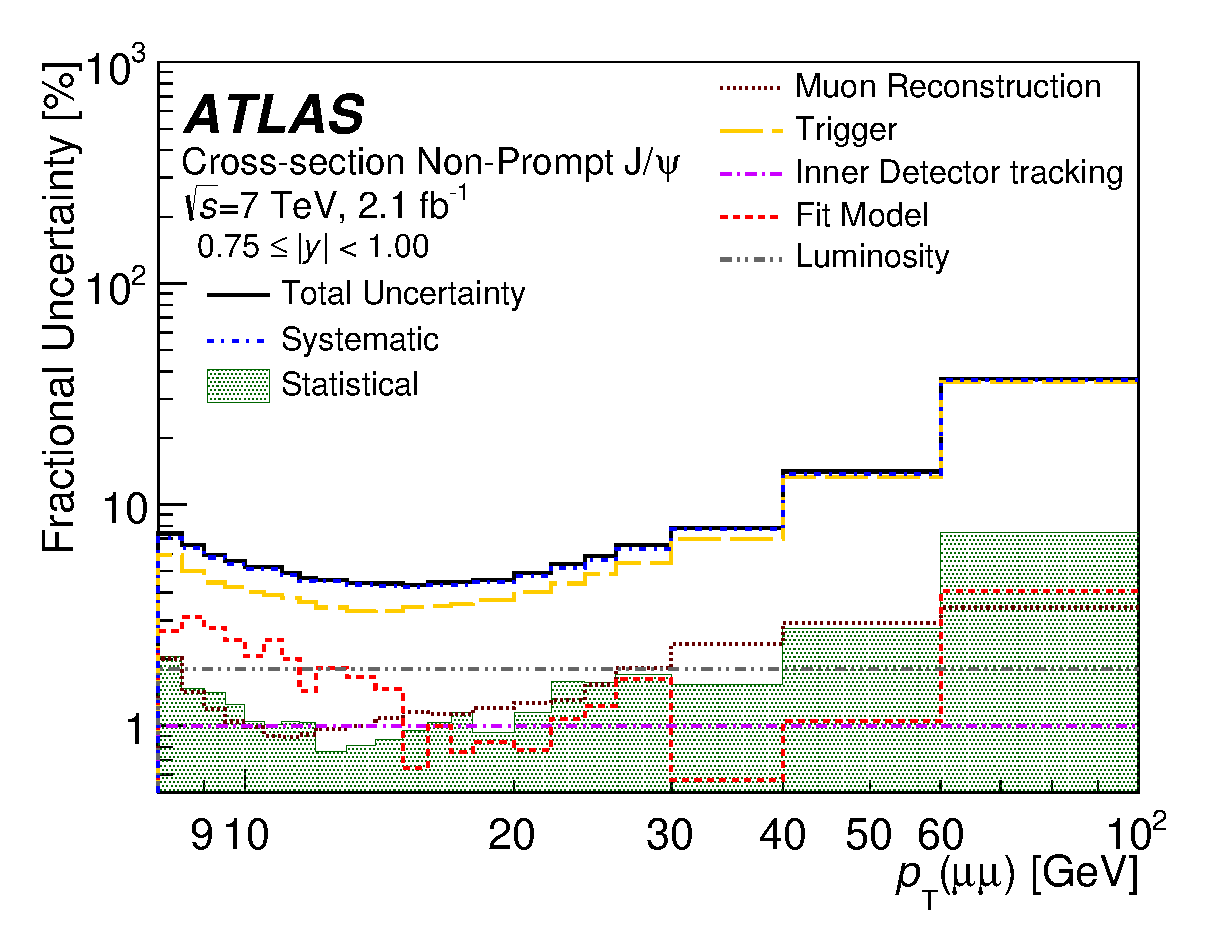
\includegraphics[width=0.49\textwidth]{hs_all_rap_0p75_1p00_jpsiNP.eps}\\
    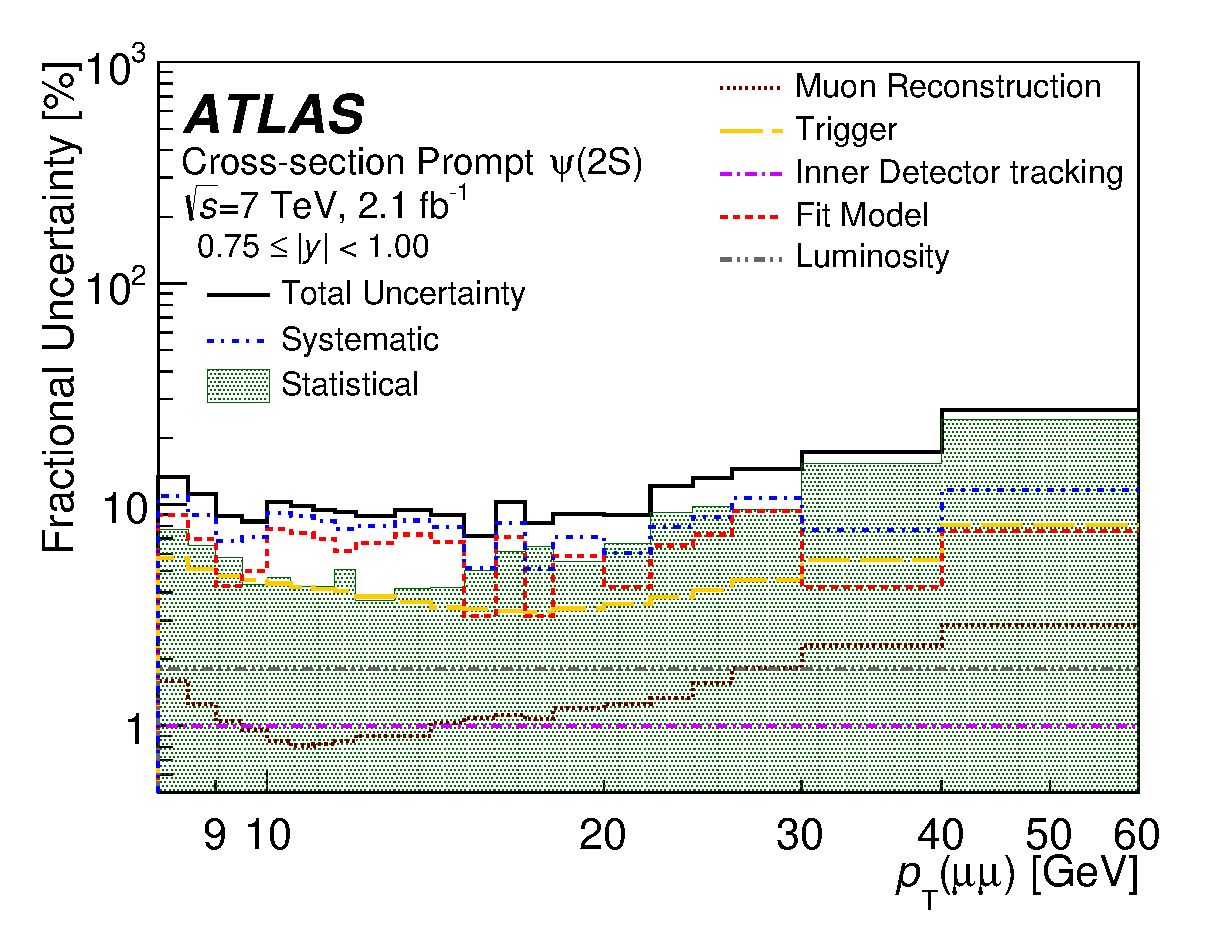
\includegraphics[width=0.49\textwidth]{hs_all_rap_0p75_1p00_psi2sP.eps}
    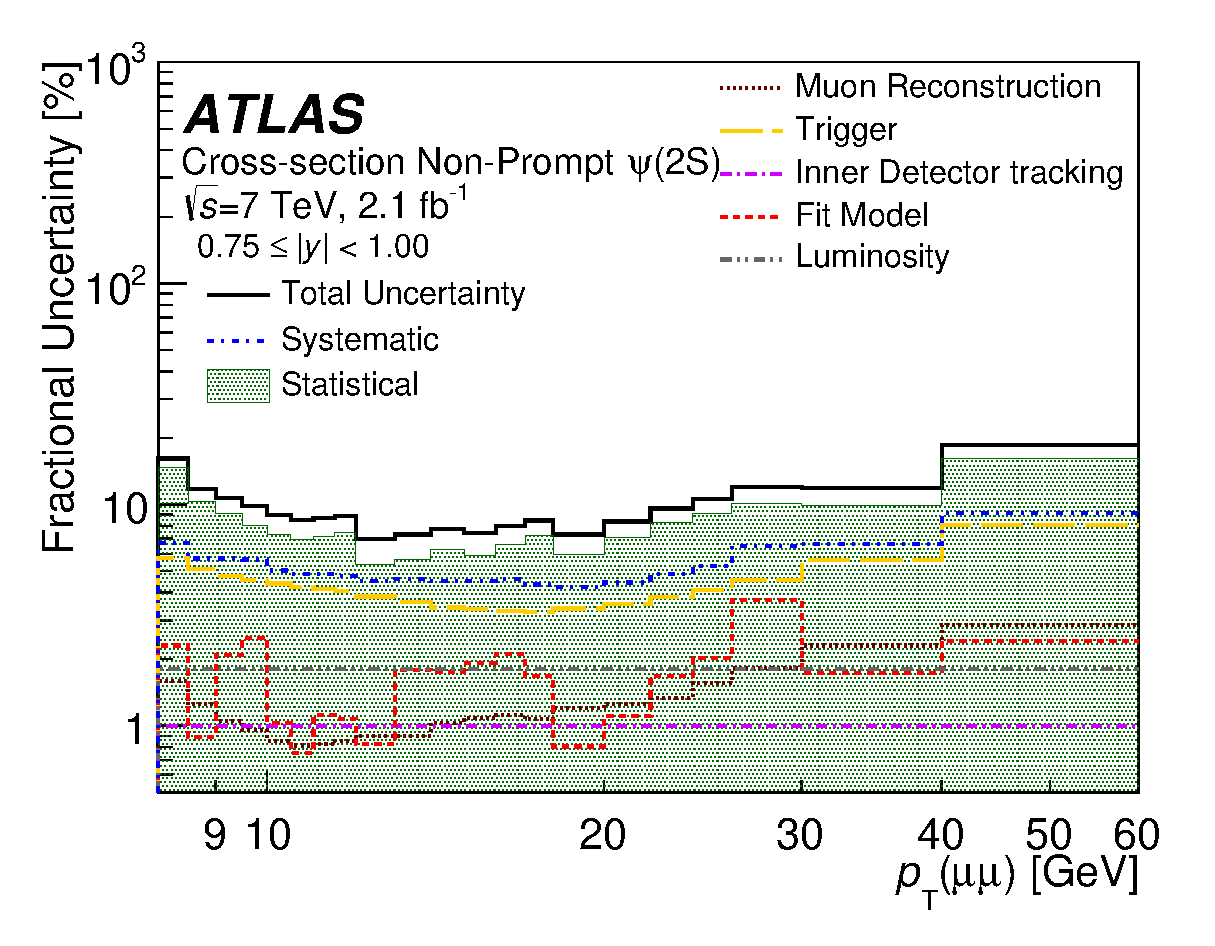
\includegraphics[width=0.49\textwidth]{hs_all_rap_0p75_1p00_psi2sNP.eps}    
    \caption{Statistical and systematic contributions to the fractional uncertainty on the prompt (left column) and non-prompt (right column)
    $\jpsi$ (top row) and $\psiprime$ (bottom row) cross-sections for 7 \TeV, 
    shown for the region $0.75<|y|<1.00$.}
    \label{fig:fracsyst_xs}
  \end{center}
\end{figure}

\begin{figure} [!h]
  \begin{center}
    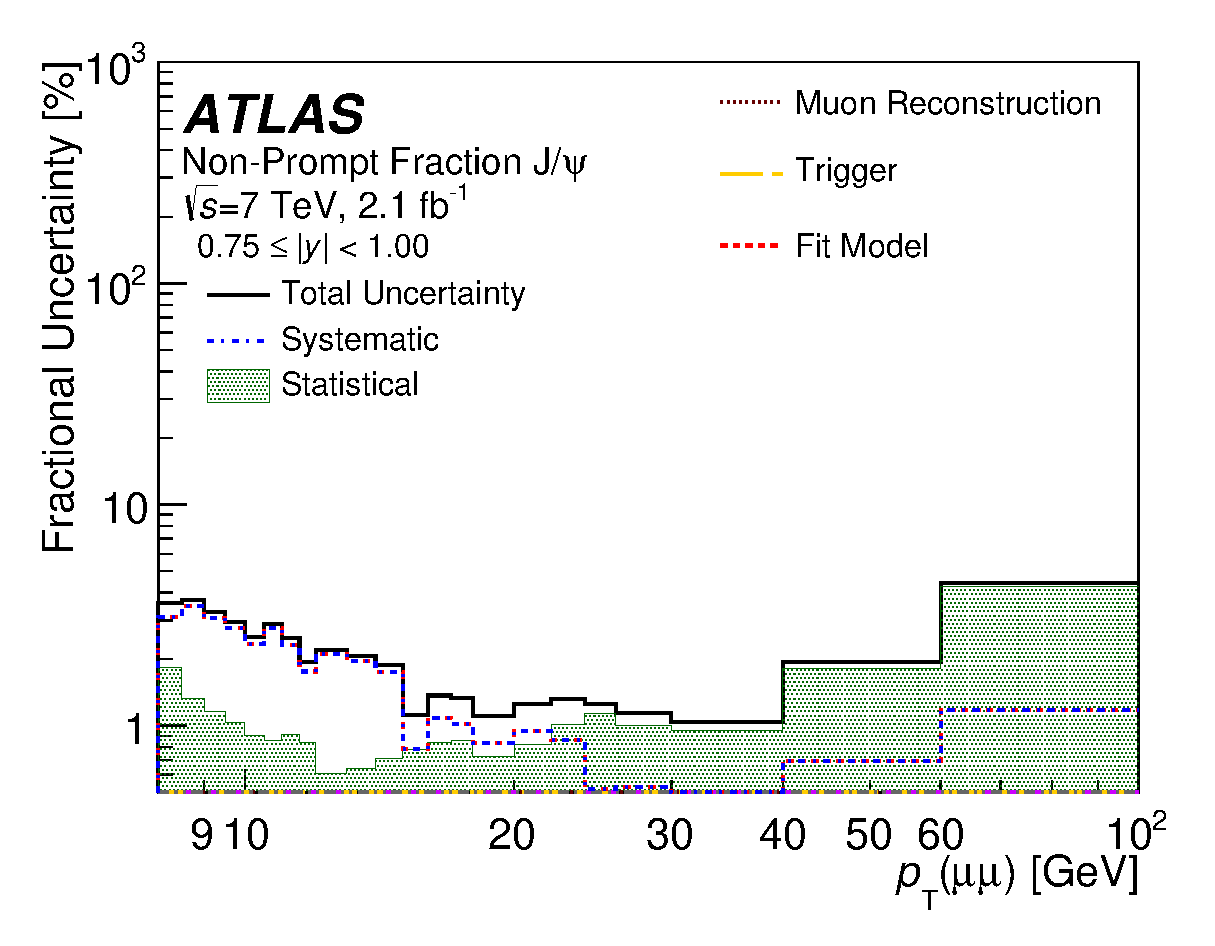
\includegraphics[width=0.49\textwidth]{hs_all_rap_0p75_1p00_fNPjpsi.eps}
    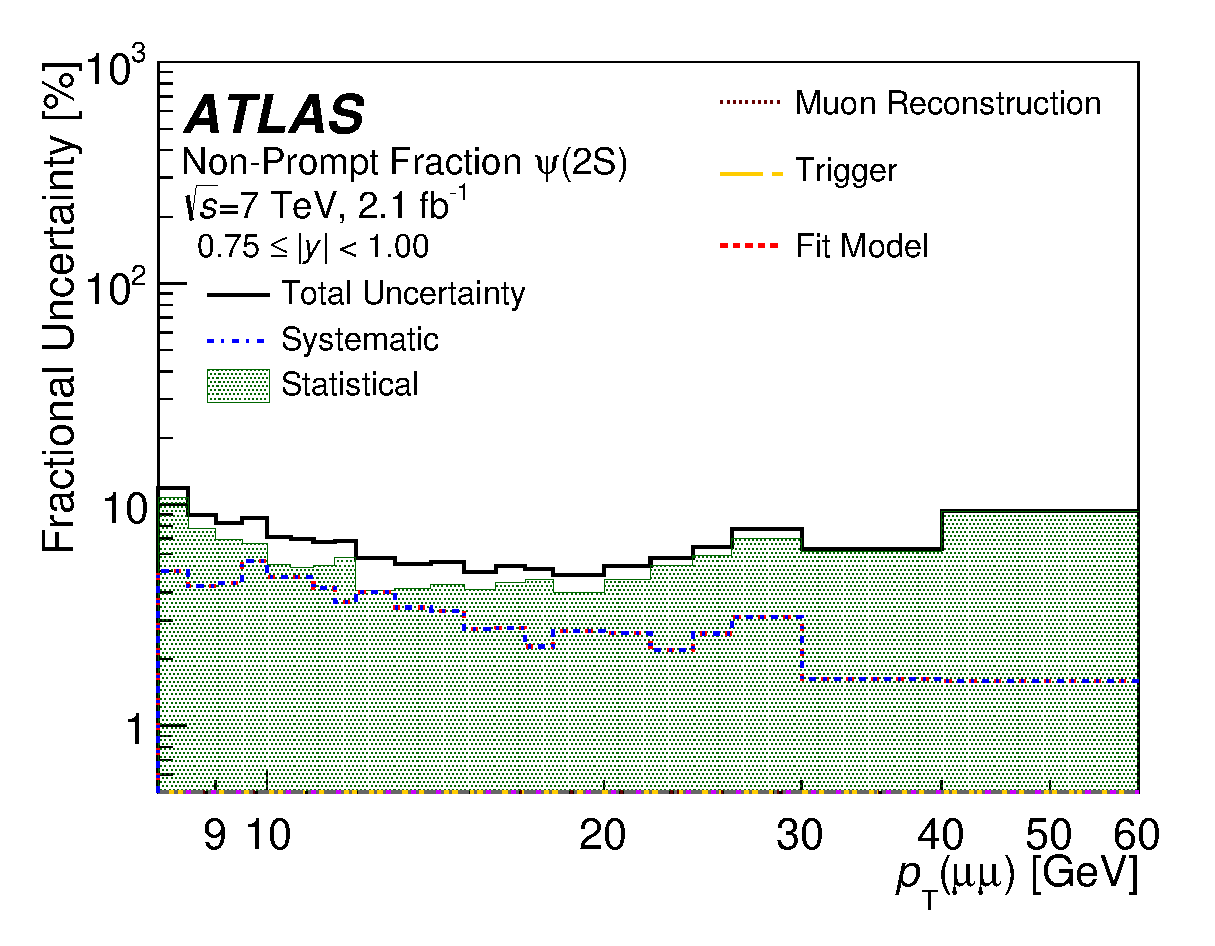
\includegraphics[width=0.49\textwidth]{hs_all_rap_0p75_1p00_fNPpsi2s.eps}\\
    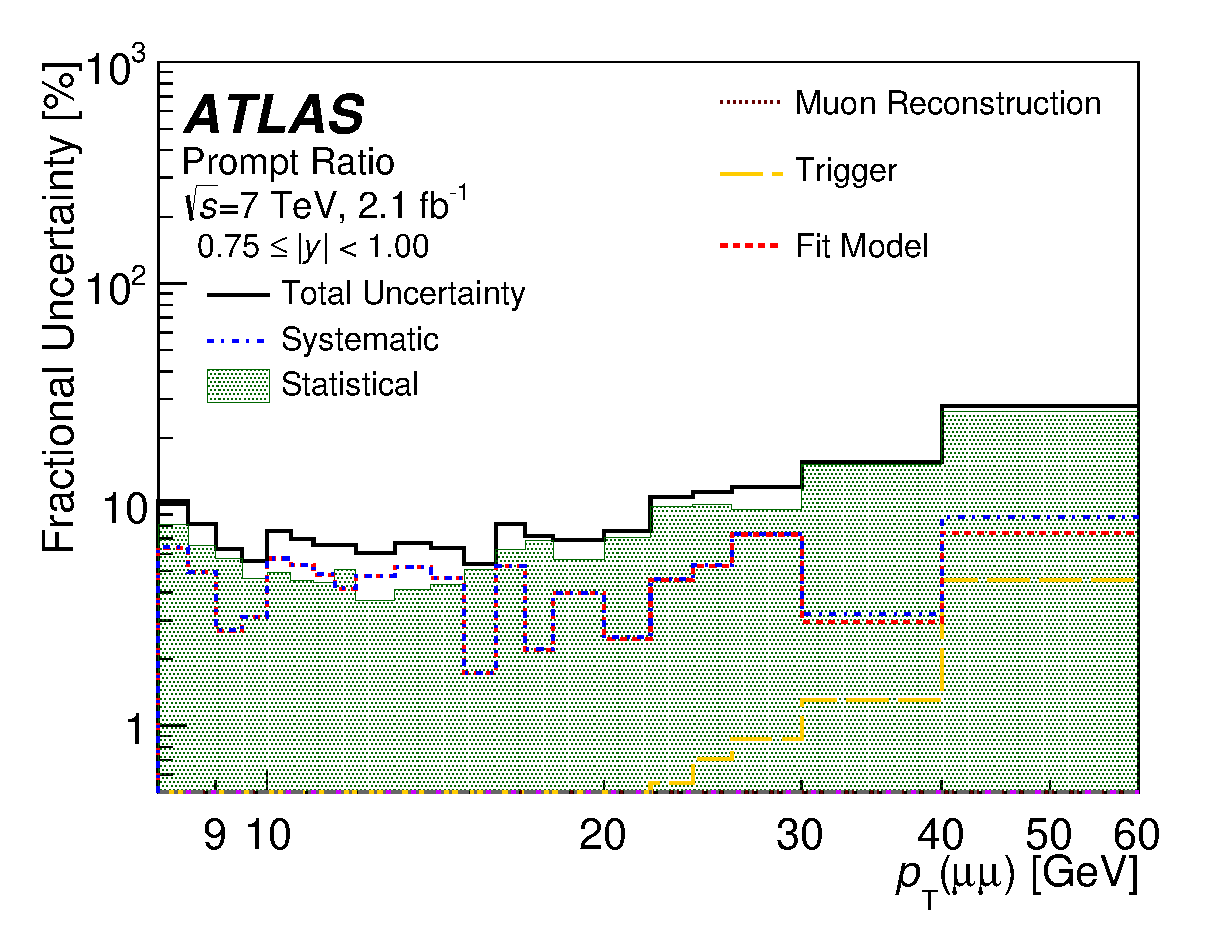
\includegraphics[width=0.49\textwidth]{hs_all_rap_0p75_1p00_ratioP.eps}
    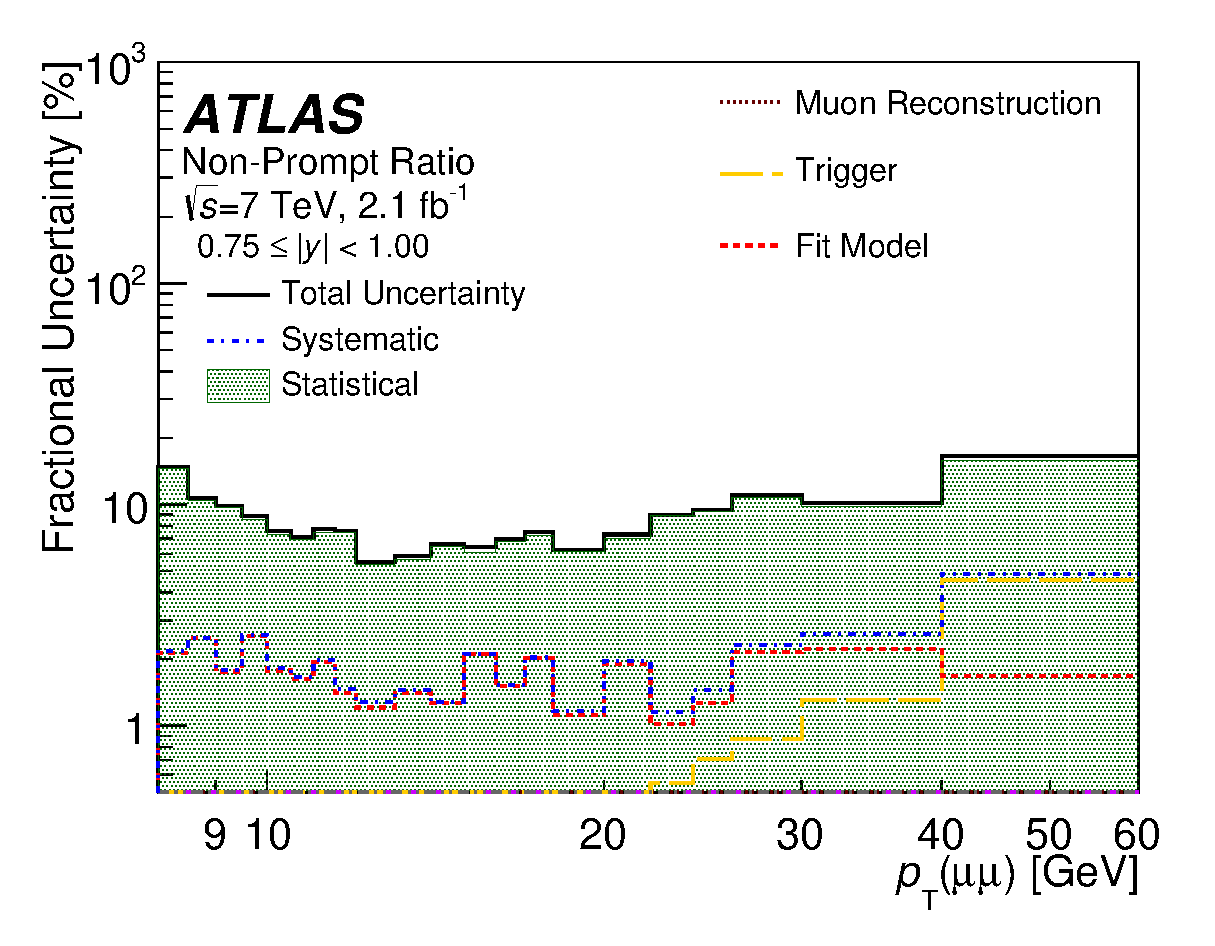
\includegraphics[width=0.49\textwidth]{hs_all_rap_0p75_1p00_ratioNP.eps} 
    \caption{Breakdown of the contributions to the fractional uncertainty on the non-prompt fractions for $\jpsi$ (top left) and $\psiprime$ (top right), 
    and the prompt (bottom left) and non-prompt (bottom right) ratios for 7 \TeV, 
    shown for the region $0.75<|y|<1.00$.}
    \label{fig:fracsyst_ratio}
  \end{center}
\end{figure}


The sources of systematic uncertainty evaluated for these measurements, along with the minimum, maximum and median values, are listed in Table~\ref{table:systlist}.
The largest contributions, which originate from the trigger and fit model uncertainties, are typically for the 
high $\pt$ intervals and are due to the limited statistics of the efficiency maps (for the trigger), and the data sample (for the fit model).

The impact of these uncertainties on the production cross-section measurements, 
as well as on their ratios for 7 \TeV\ data, is shown for a representative interval in
Figures~\ref{fig:fracsyst_xs} and~\ref{fig:fracsyst_ratio}, respectively.
The impact is very similar at 8 \TeV.


\begin{table}[h!]
 \caption{Summary of the minimum and maximum contributions along with the median of the systematic uncertainties as percentages. Values are quoted for 7 and 8 \TeV\ data.}
 \centering
    \begin{tabular}{l || c c c | c c c  }
    \hline 
     & \multicolumn{3}{c|}{7 \TeV\ [\%]} & \multicolumn{3}{c}{8 \TeV\ [\%]} \\
    \hline 
    Source of systematic uncertainty                   & Min & Median & Max & Min & Median & Max \\
    Luminosity                         & 1.8 & 1.8 & 1.8    & 2.8 & 2.8 & 2.8 \\
    Muon reconstruction efficiency     & 0.7 & 1.2 & 4.7    & 0.3 & 0.7 & 6.0 \\
    Muon trigger efficiency            & 3.2 & 4.7 & 35.9   & 2.9 & 7.0 & 23.4 \\
    Inner detector tracking efficiency & 1.0 & 1.0 & 1.0    & 1.0 & 1.0 & 1.0 \\
    Fit model parameterizations        & 0.5 & 2.2 & 22.6   & 0.26 & 1.07 & 24.9 \\
    Bin migrations                     & 0.01 & 0.1 & 1.4   & 0.01 & 0.3 & 1.5 \\ \hline
    Total                              & 4.2 & 6.5  & 36.3  & 4.4 & 8.1 & 27.9 \\
    \hline  
      \hline
    \end{tabular}
\label{table:systlist}
\end{table}


\setdescription{font=\normalfont\itshape}

\begin{description}[style=unboxed,leftmargin=0cm]
\item[Luminosity] \hfill \\
The uncertainty on the integrated luminosity is $1.8\%$ ($2.8\%$) for the 7~\TeV\ (8~\TeV) data-taking period.  
The methodology used to determine these uncertainties is described in Ref.~\cite{Aad:2013ucp}.
The luminosity uncertainty is only applied to the \jpsi\ and \psiprime\ cross-section results.


\item[Muon reconstruction and trigger efficiencies] \hfill \\
To determine the systematic uncertainty on the muon reconstruction and trigger efficiency maps, each of the maps is reproduced in 100 pseudo-experiments.
The dominant uncertainty in each bin is statistical and hence any bin-to-bin correlations are neglected.
For each pseudo-experiment a new map is created by varying independently each bin content according to a Gaussian distribution about its estimated value, 
determined from the original map.
In each pseudo-experiment, the total weight is recalculated for each dimuon $\pt$ and $|y|$ interval of the analysis.
The RMS of the total weight pseudo-experiment distributions for each efficiency type is used as the systematic uncertainty,
where any correlation effects between the muon and trigger efficiencies can be neglected.


The ID tracking efficiency is in excess of $99.5\%$ \cite{Aad2012dlq}, and
an uncertainty of 1\% is applied to account for the ID dimuon reconstruction inefficiency (0.5\% per muon, added coherently). This
uncertainty is applied to the differential cross-sections and is assumed to cancel in the ratio of non-prompt to inclusive production for \jpsi\ and 
\psiprime\ and in the ratios of \psiprime\ to \jpsi\ production.

For the trigger efficiency  $\epsilon_\mathrm{trig}$, there is an additional correction that accounts for correlations between the two trigger muons. This 
correction is varied by its uncertainty, and the shift in the resultant total weight relative to its central value is added in quadrature to the uncertainty from the map.
The choice of triggers is known \cite{Aad:2014cqa} to introduce a small lifetime-dependent efficiency loss but it is determined to have a negligible effect on 
the prompt and non-prompt yields and no correction is applied in this analysis.

  \item[Fit model uncertainty] \hfill \\
The uncertainty due to the fit procedure is determined by varying one component at a
time in the fit model described in Section \ref{sec:method:fit}, creating a set of new fit models. For each new
fit model, all measured quantities are recalculated, and in each $\pt$ and $|y|$ interval the spread of
variations around the central fit model is used as its systematic uncertainty.
The following variations to the central model fit are evaluated: 

\begin{itemize}

  \item  signal mass model --- using double Gaussian models in place of the Crystal Ball plus Gaussian model;  variation of the
 $\alpha$ and $n$ parameters of the $B$ model, which are originally fixed;

    \item  signal pseudo-proper decay time model --- a double exponential function is used to describe the pseudo-proper decay time distribution for the 
    $\apsi$ non-prompt signal;

  \item  background mass models --- variations of the mass model using exponentials functions, or quadratic Chebyshev polynomials to describe the components of prompt,
 non-prompt and double-sided background terms;

  \item  background pseudo-proper decay time model --- a single exponential function was considered for the non-prompt component;

  \item  pseudo-proper decay time resolution model --- using a single Gaussian function in place of the double Gaussian function to model the lifetime resolution
 (also prompt lifetime model); and variation of the mixing terms for the two Gaussian components of this term.

\end{itemize}

  \item[Bin migrations] \hfill \\
As the corrections to the results due to bin migration effects are factors close to unity in all regions, the difference between the correction factor and unity is applied as the uncertainty. 

\end{description}




\section{Results}
\label{sec:results}


The $\jpsi$ and $\psiprime$ non-prompt and prompt production cross-sections are presented, corrected for acceptance and detector efficiencies 
while assuming isotropic decay, as described in Section~\ref{sec:s:diff_xSecDet}. 
Also presented are the ratios of non-prompt production relative to the inclusive production for $\jpsi$ and $\psiprime$ mesons separately, described in Section~\ref{sec:s:NPFDet},
and the ratio of $\psiprime$ to $\jpsi$ production for prompt and non-prompt components separately, described in Section~\ref{sec:s:PNPRatioDet}.
Correction factors for various spin-alignment hypotheses for both 7 and 8~\TeV\  data can be found in 
Tables~\ref{tab:sa_long_jpsi}--\ref{tab:sa_offN_psi2s} (in Appendix) and Tables~\ref{tab:sa_long_jpsi8}--\ref{tab:sa_offN_psi2s8} (in Appendix) respectively, in terms of 
\pt\ and rapidity intervals.

\setdescription{font=\normalfont\itshape}

\begin{description}[style=unboxed,leftmargin=0cm]


\item[Production cross-sections] \hfill

Figures \ref{fig:res:xSecP} and \ref{fig:res:xSecNP} show respectively the prompt and non-prompt 
differential cross-sections of \jpsi\ and \psiprime\ as functions of $\pt$ and $|y|$, together with the relevant theoretical predictions, 
which are described below.


\begin{figure} [!ht]
  \begin{center}
    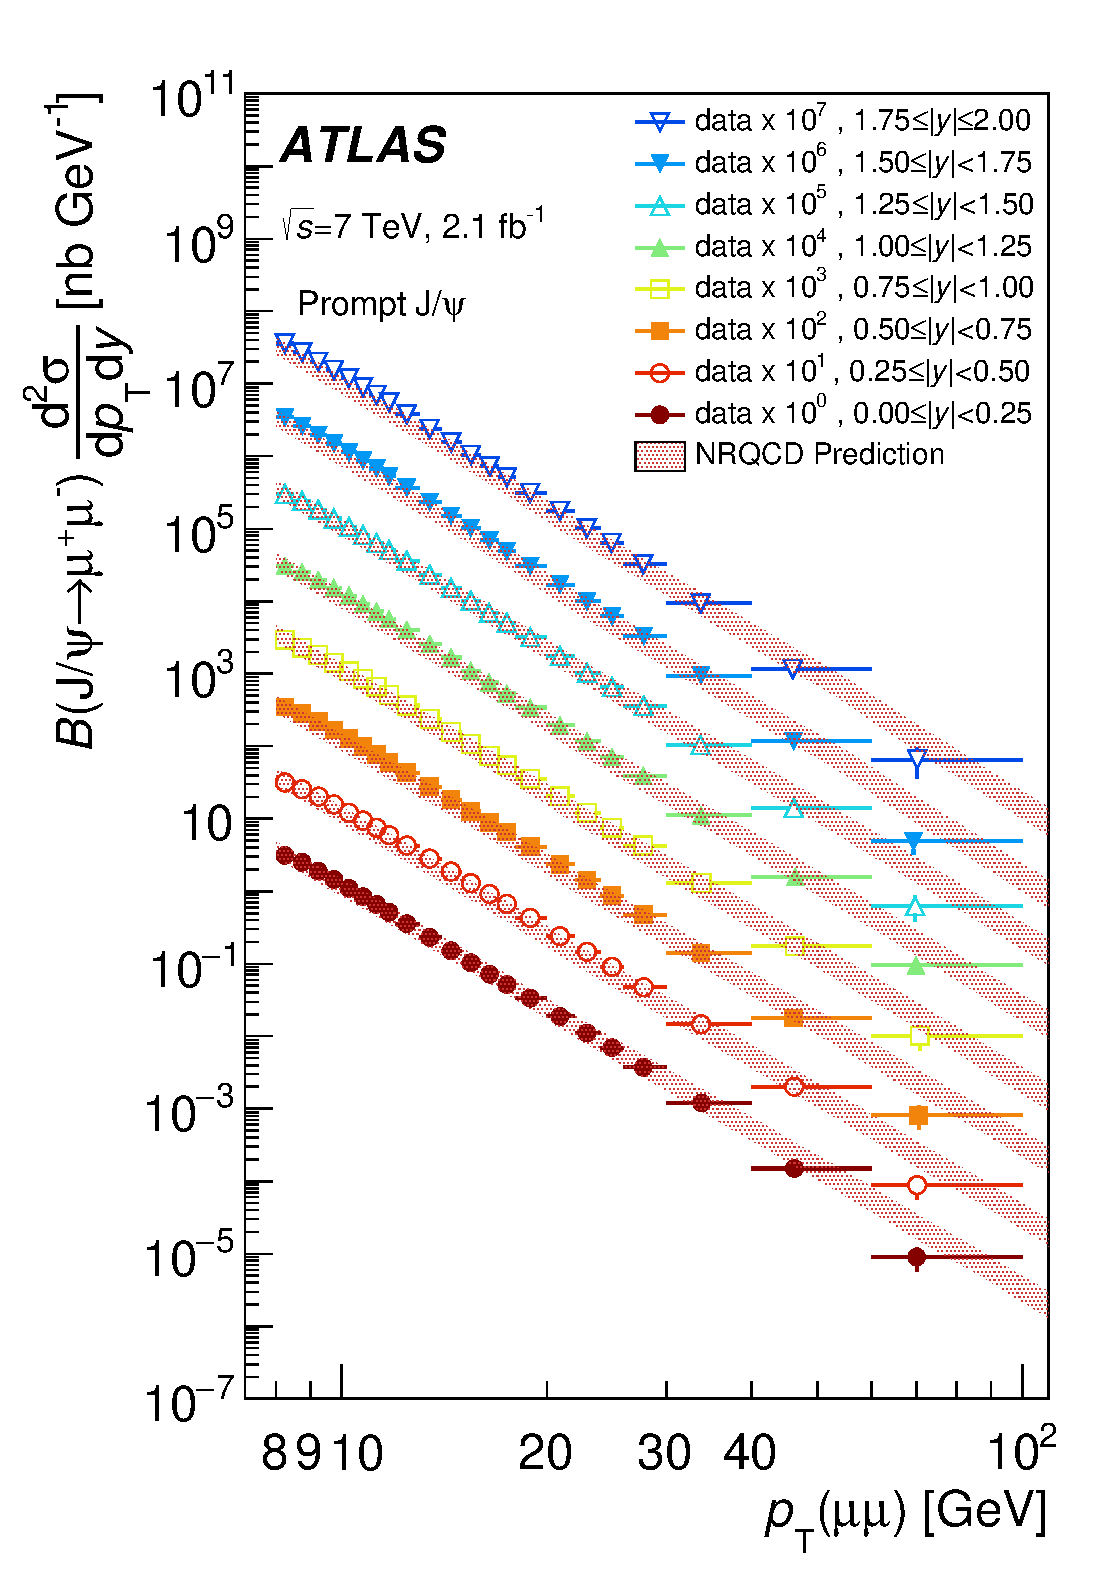
\includegraphics[width=0.44\textwidth]{figures/ct_7TeV_JpsiP_xSec.eps} 
    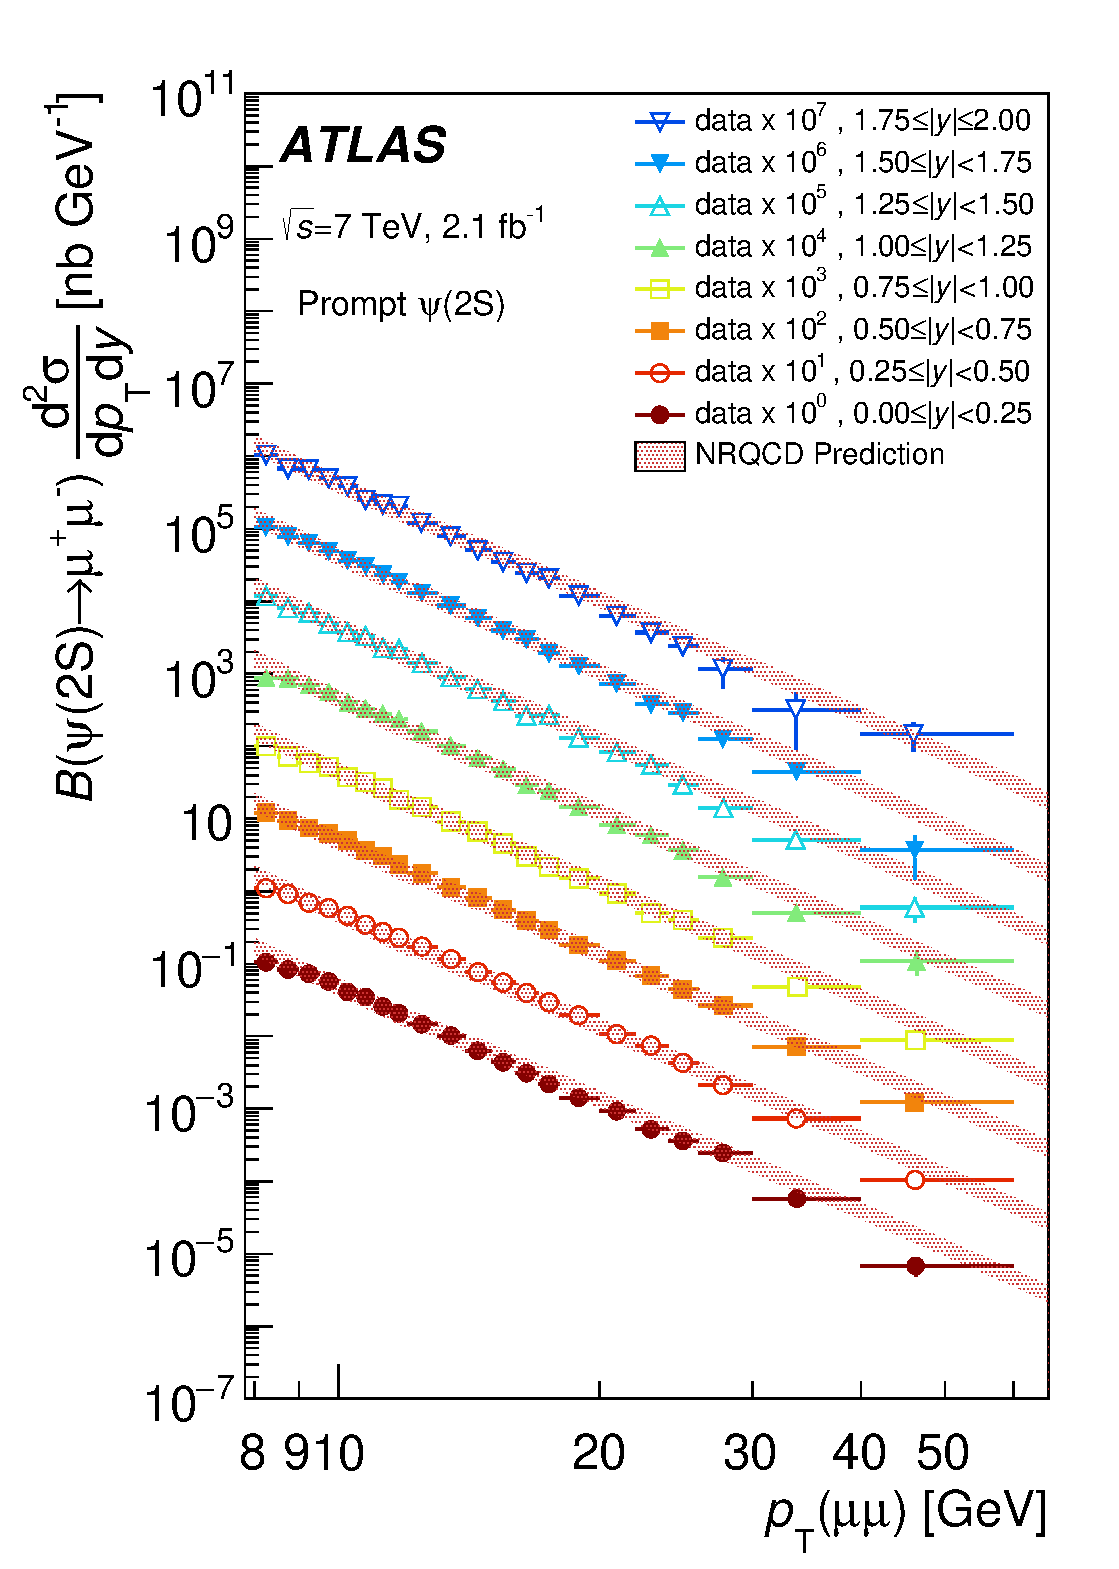
\includegraphics[width=0.44\textwidth]{figures/ct_7TeV_Psi2SP_xSec.eps}\hfil\\
    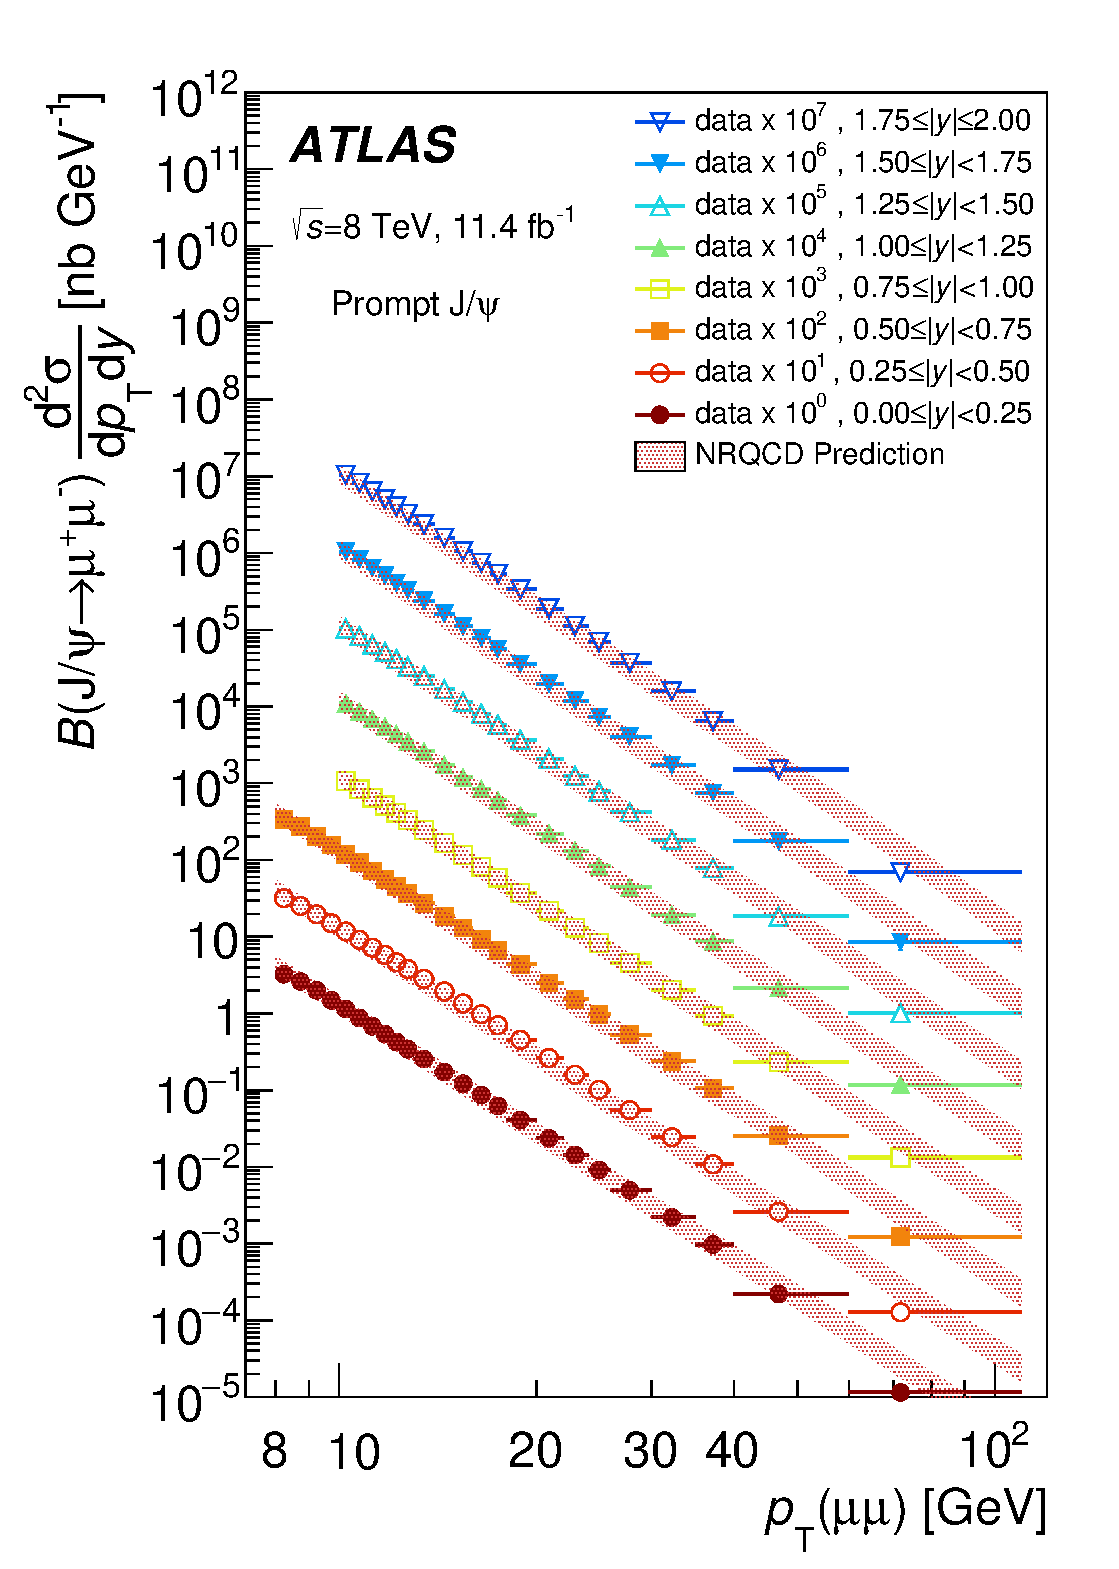
\includegraphics[width=0.44\textwidth]{figures/ct_8TeV_JpsiP_xSec.eps}
    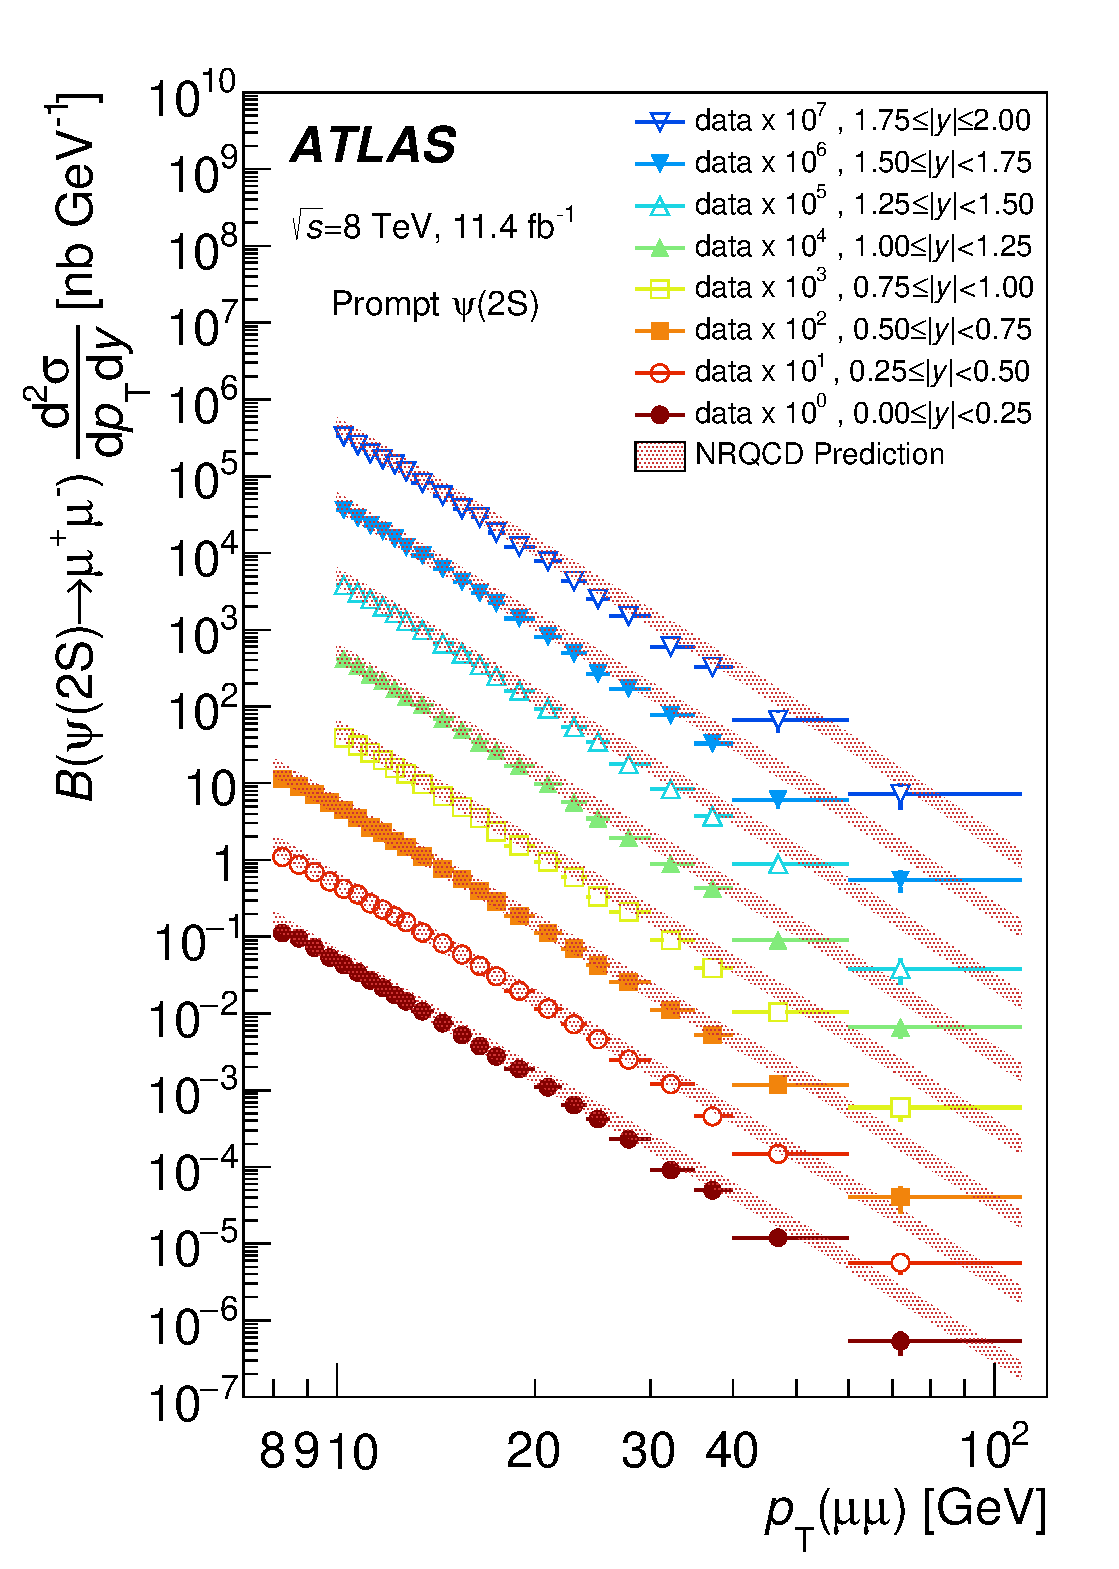
\includegraphics[width=0.44\textwidth]{figures/ct_8TeV_Psi2SP_xSec.eps}\hfil
    \caption{The differential prompt cross-section times dimuon branching fraction of \jpsi\ (left) and \psiprime\ (right) as a function 
    of $\pt(\mu\mu)$ for each slice of rapidity. 
    The top (bottom) row shows the 7~\TeV\ (8~\TeV) results.
    For each increasing rapidity slice, an additional scaling factor of 10 is applied to the plotted points for visual clarity. The
      centre of each bin on the horizontal axis represents the mean of the weighted $\pt$ distribution. The
      horizontal error bars represent the range of $\pt$ for the bin, and the vertical error bar covers 
      the statistical and systematic 
      uncertainty (with the same multiplicative scaling applied). 
      The NLO NRQCD theory predictions are also shown.}
    \label{fig:res:xSecP}
  \end{center}
\end{figure} 

\begin{figure} [!ht]
  \begin{center} 
    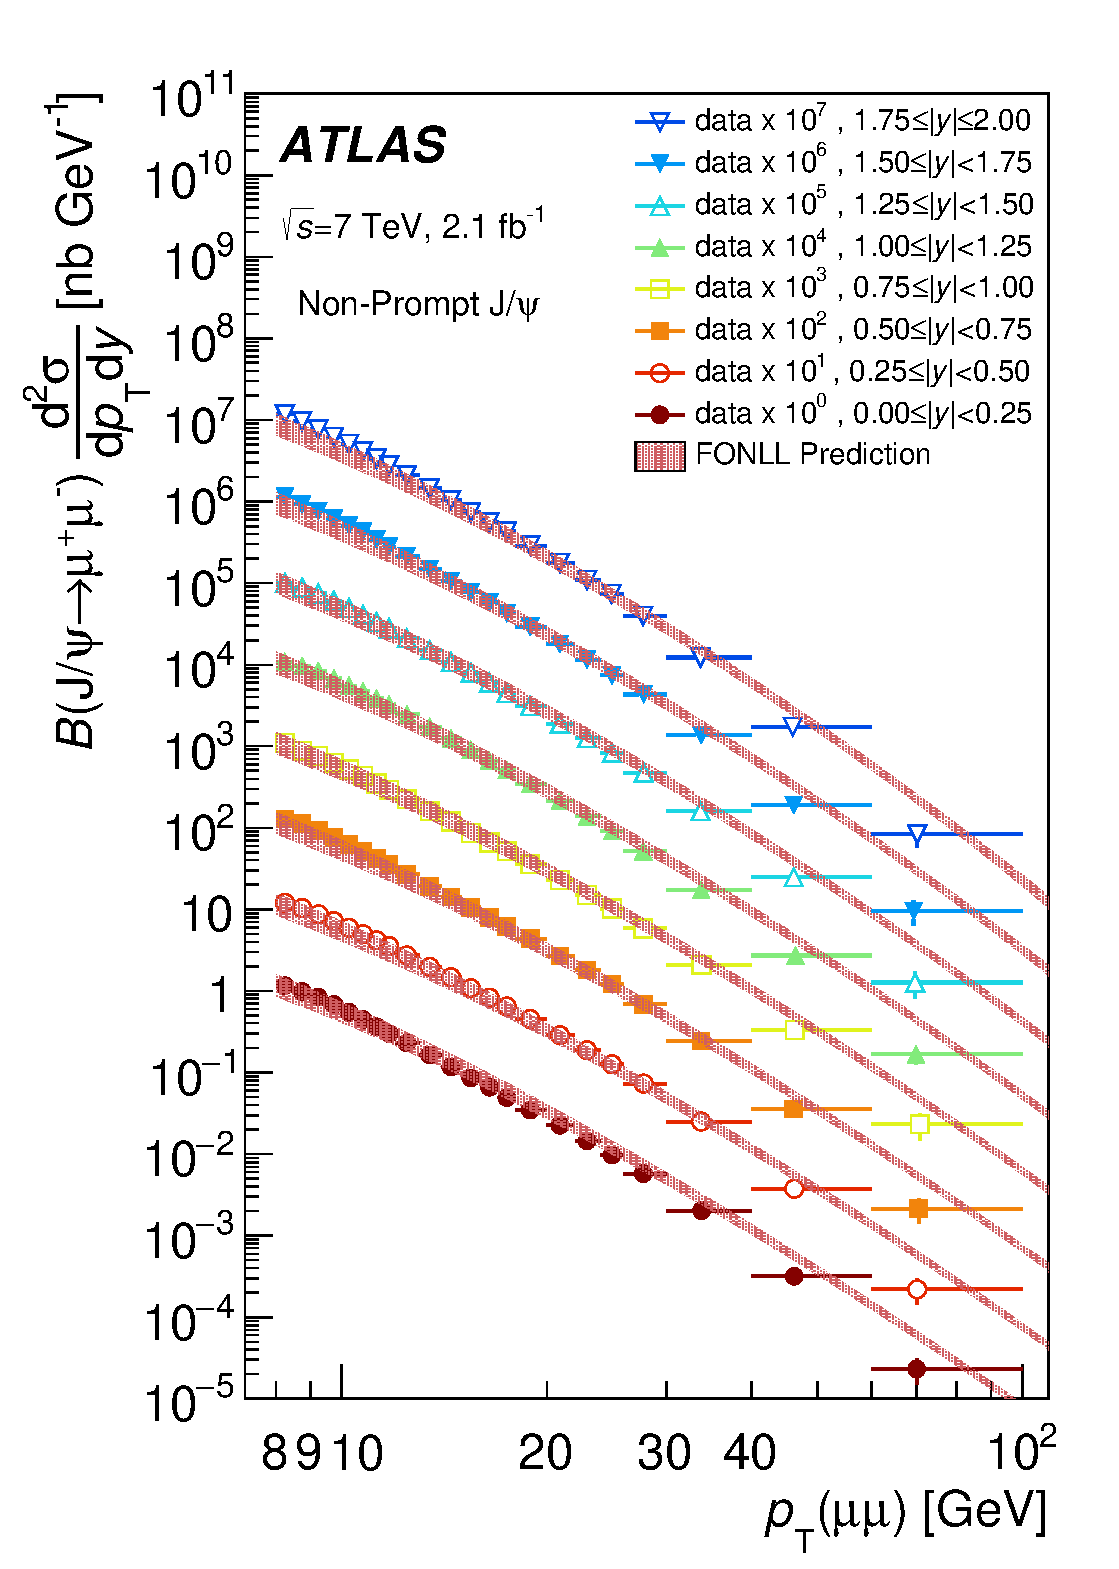
\includegraphics[width=0.44\textwidth]{figures/ct_7TeV_JpsiNP_xSec.eps}
    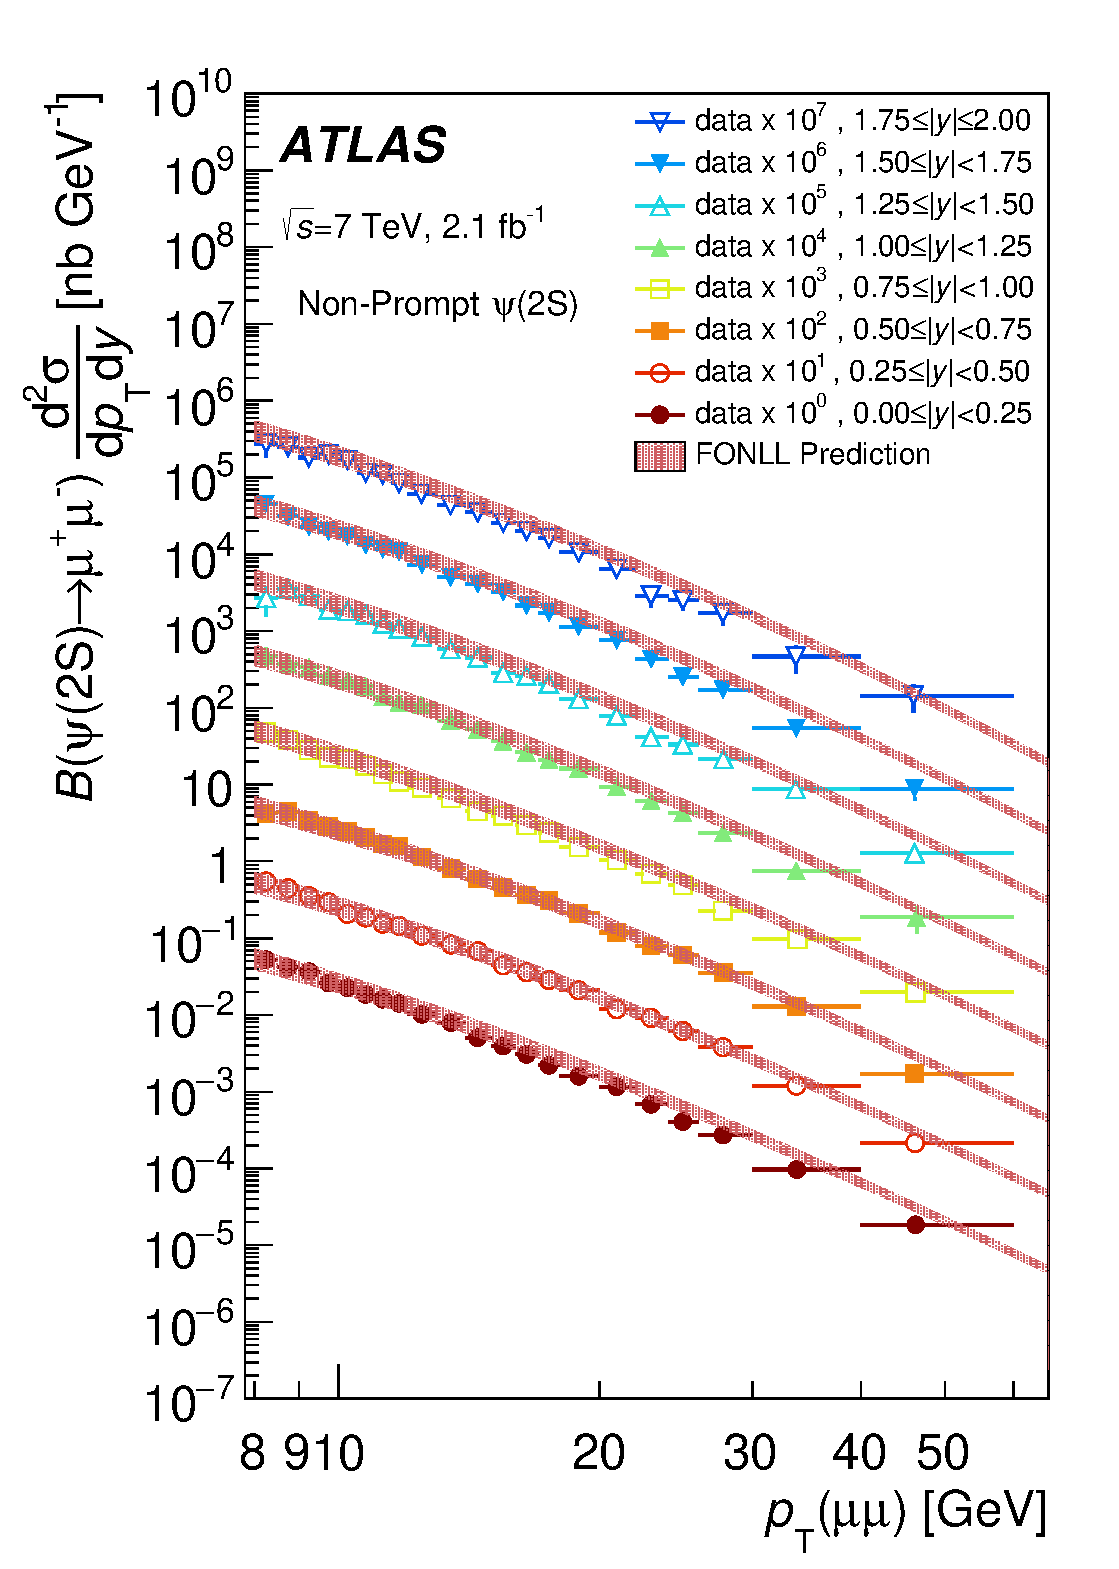
\includegraphics[width=0.44\textwidth]{figures/ct_7TeV_Psi2SNP_xSec.eps}\hfil
    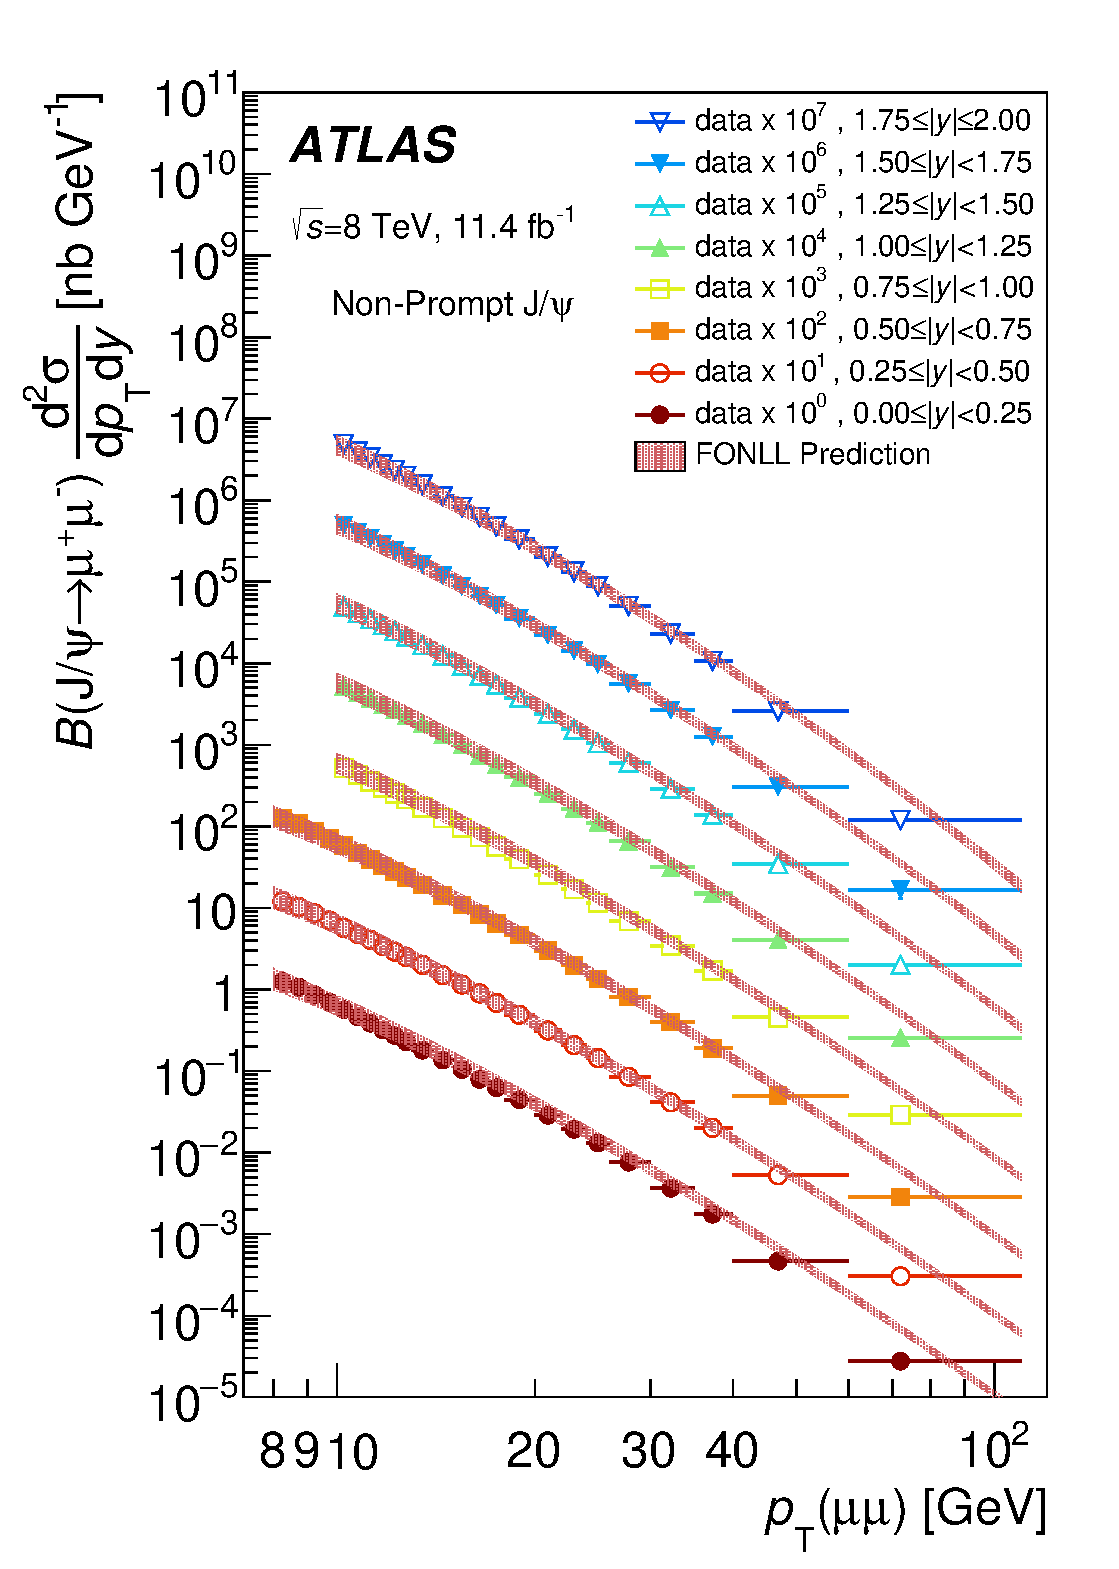
\includegraphics[width=0.44\textwidth]{figures/ct_8TeV_JpsiNP_xSec.eps}
    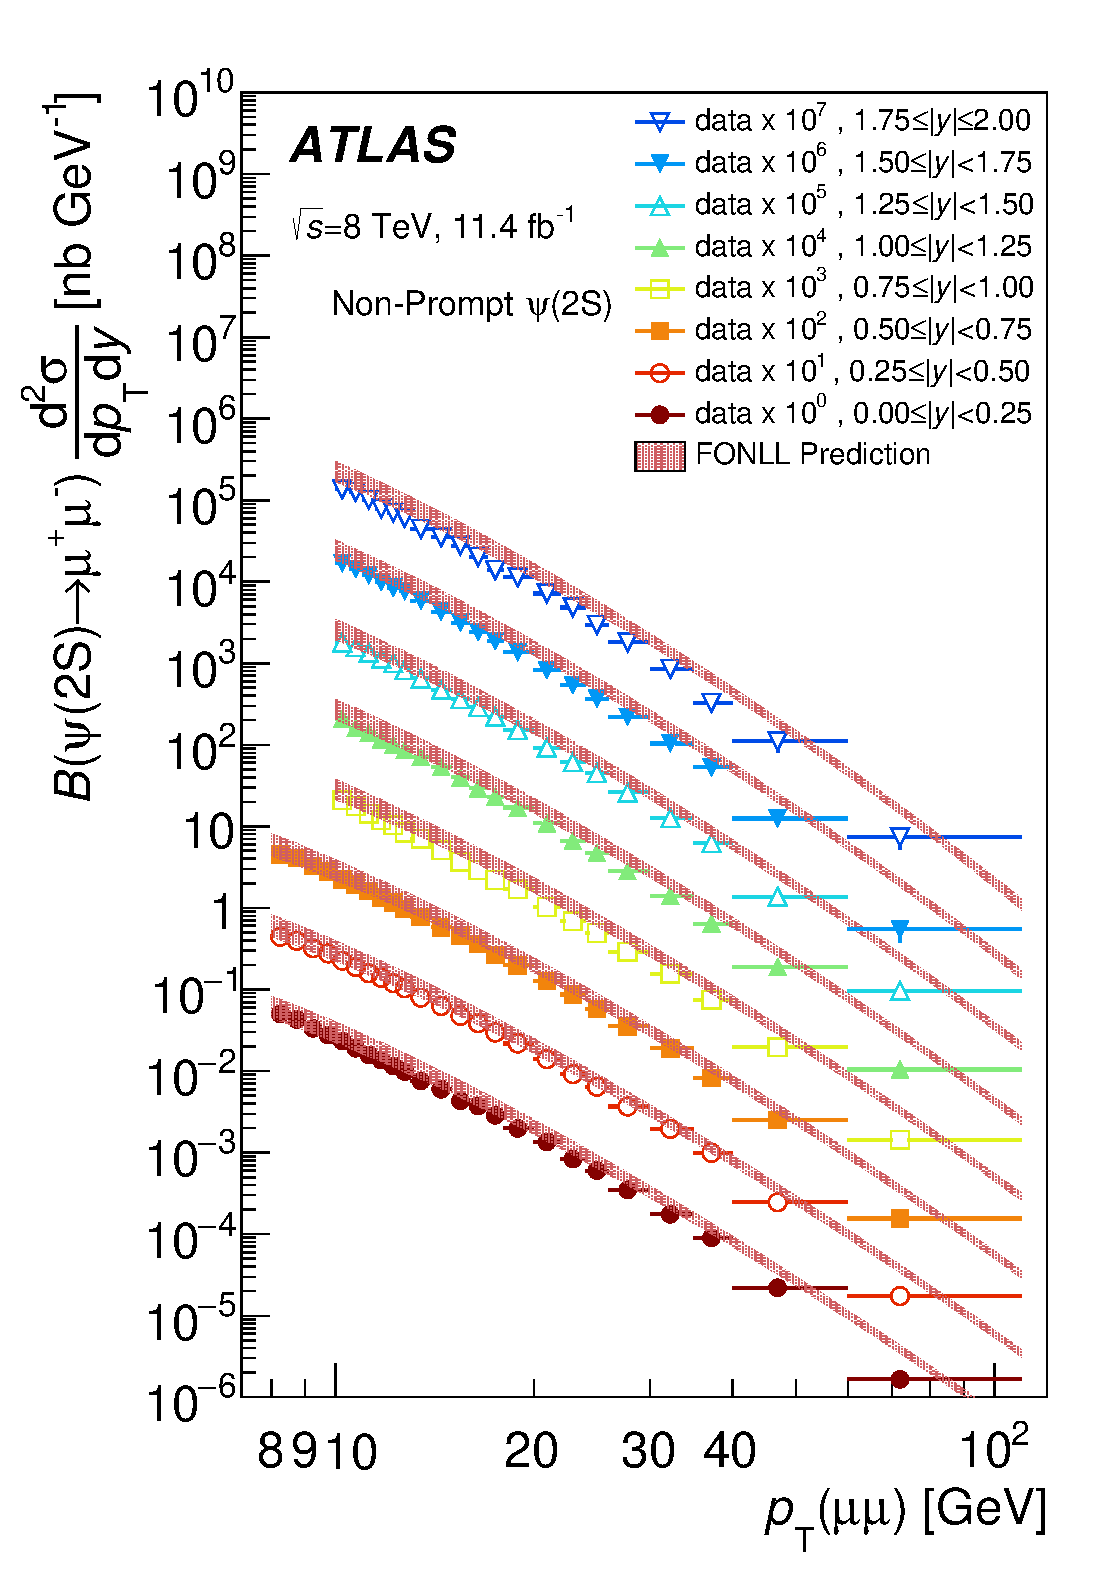
\includegraphics[width=0.44\textwidth]{figures/ct_8TeV_Psi2SNP_xSec.eps}\hfil
    \caption{The differential non-prompt cross-section times dimuon branching fraction of \jpsi\ (left) and \psiprime\ (right) as a function 
    of $\pt(\mu\mu)$ for each slice of rapidity. 
    The top (bottom) row shows the 7~\TeV\ (8~\TeV) results.
    For each increasing rapidity slice, an additional scaling factor of 10 is applied to the plotted points for visual clarity. The
      centre of each bin on the horizontal axis represents the mean of the weighted $\pt$ distribution. The
      horizontal error bars represent the range of $\pt$ for the bin, and the vertical error bar covers the statistical
      and systematic uncertainty (with the same multiplicative scaling applied).
      The FONLL theory predictions are also shown.}
    \label{fig:res:xSecNP}
  \end{center}
\end{figure} 


\item[Non-prompt production fractions] \hfill % \\

The results for the fractions of non-prompt production relative to the inclusive production of \jpsi\ and \psiprime\, are presented as a function of $\pt$ for slices of rapidity in Figure~\ref{fig:res:NPF}. 
In each rapidity slice, the non-prompt fraction is seen to increase as a function of $\pt$ and has no strong dependence on either rapidity or centre-of-mass energy.

\begin{figure} [!ht]
  \begin{center}
    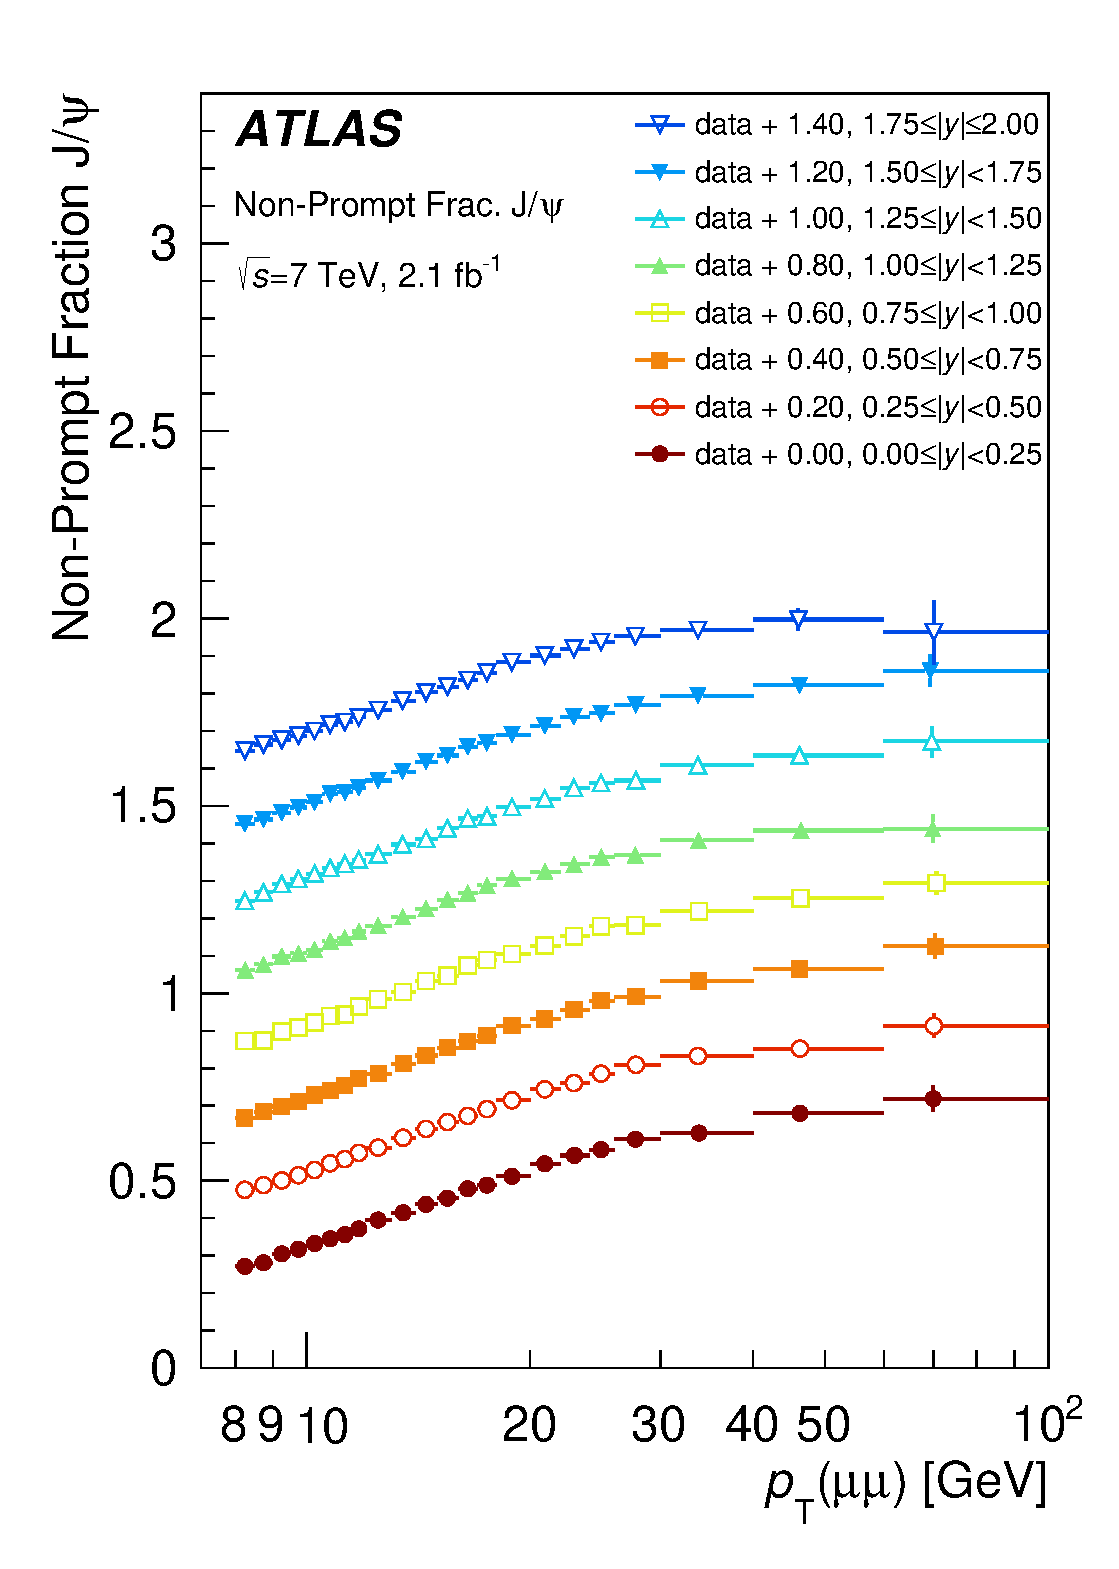
\includegraphics[width=0.44\textwidth]{figures/ct_7TeV_NPF_Jpsi.eps} 
    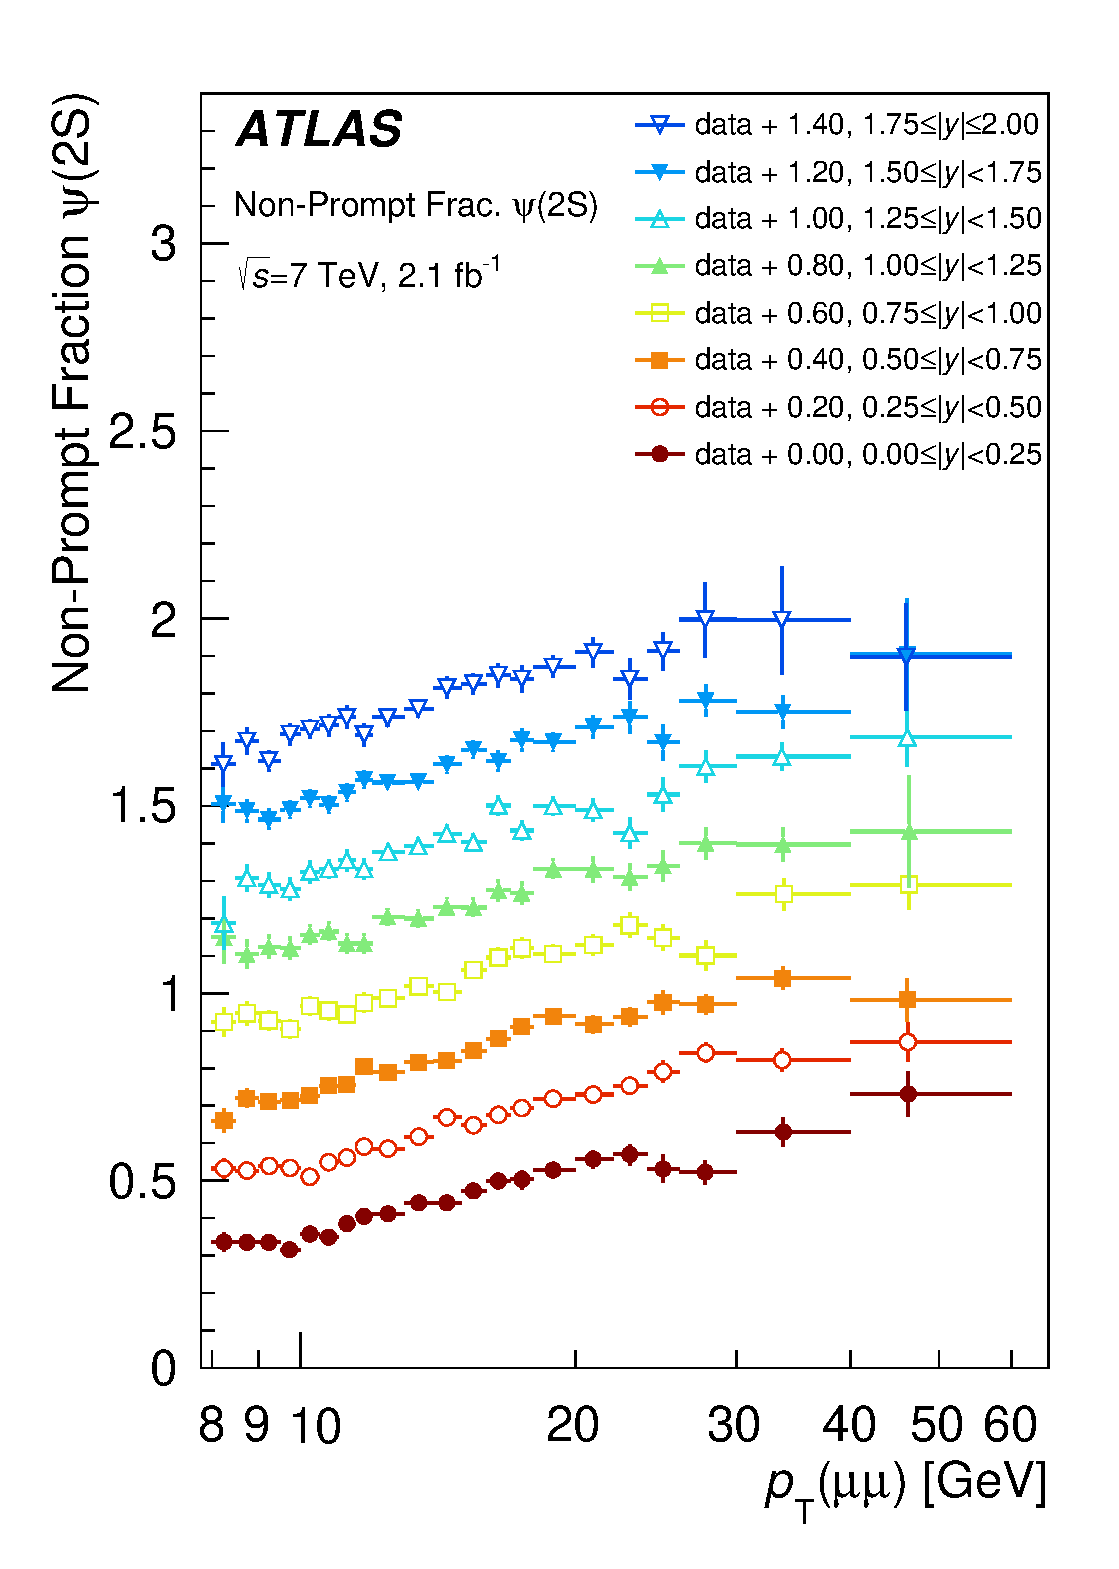
\includegraphics[width=0.44\textwidth]{figures/ct_7TeV_NPF_Psi.eps}\hfil\\
    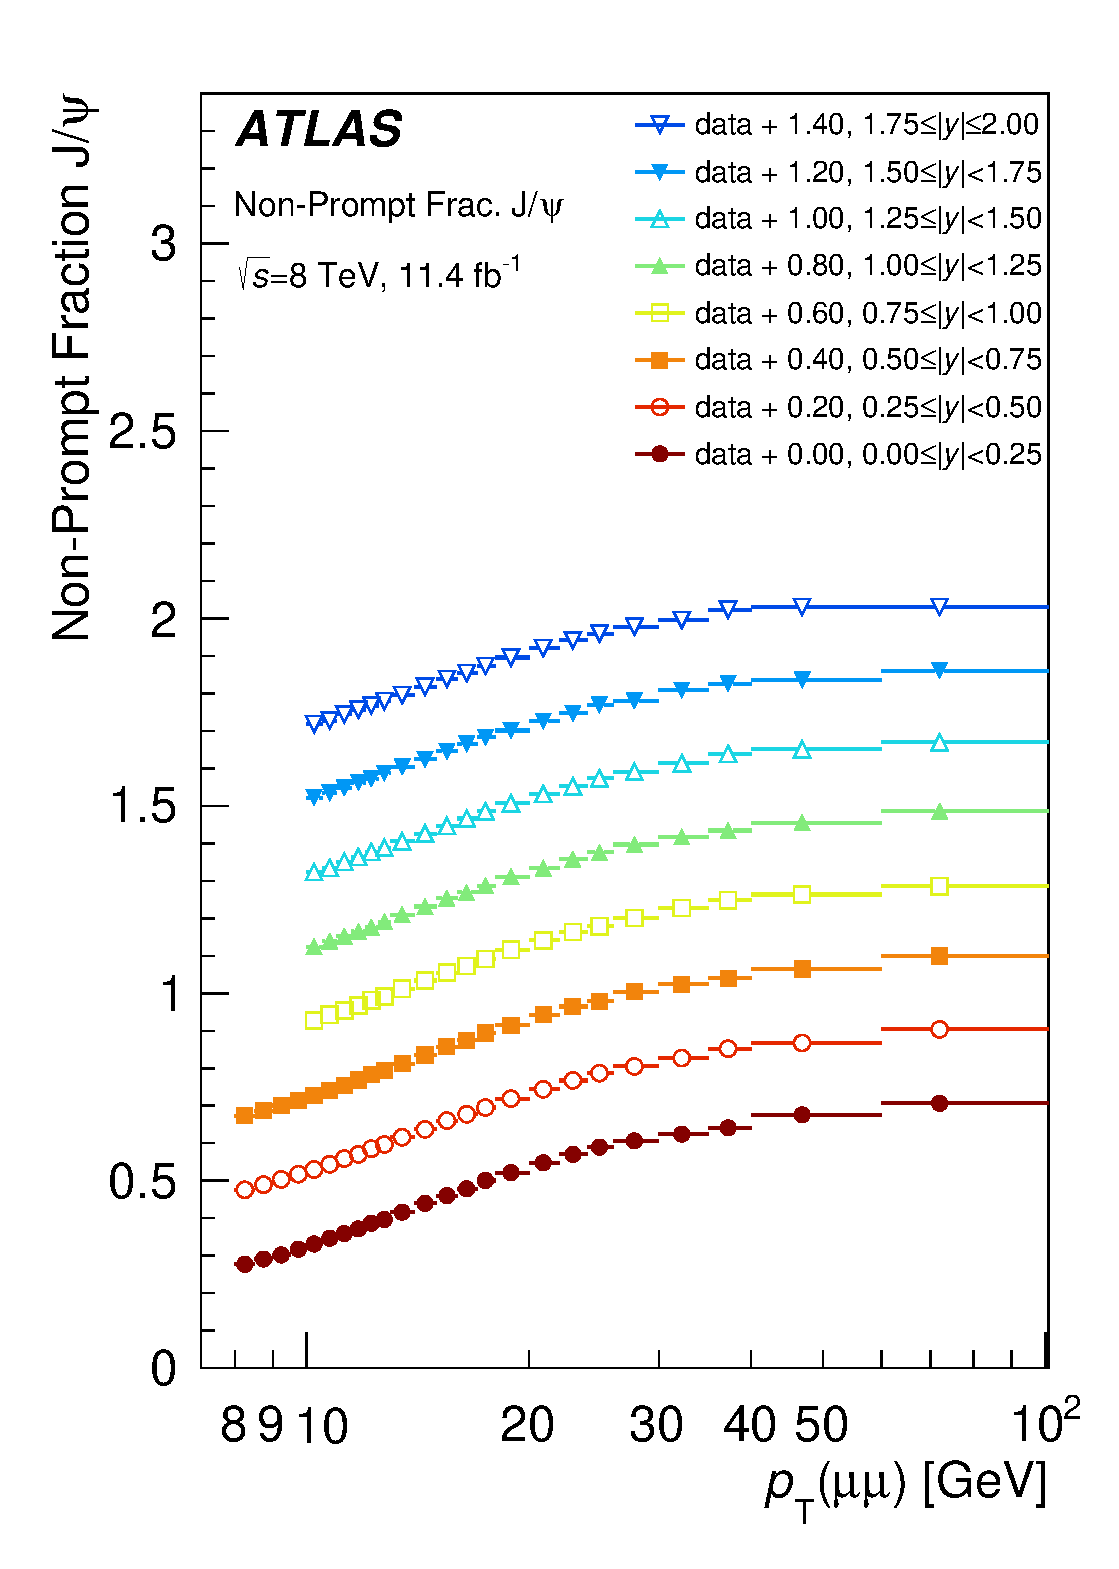
\includegraphics[width=0.44\textwidth]{figures/ct_8TeV_NPF_Jpsi.eps}
    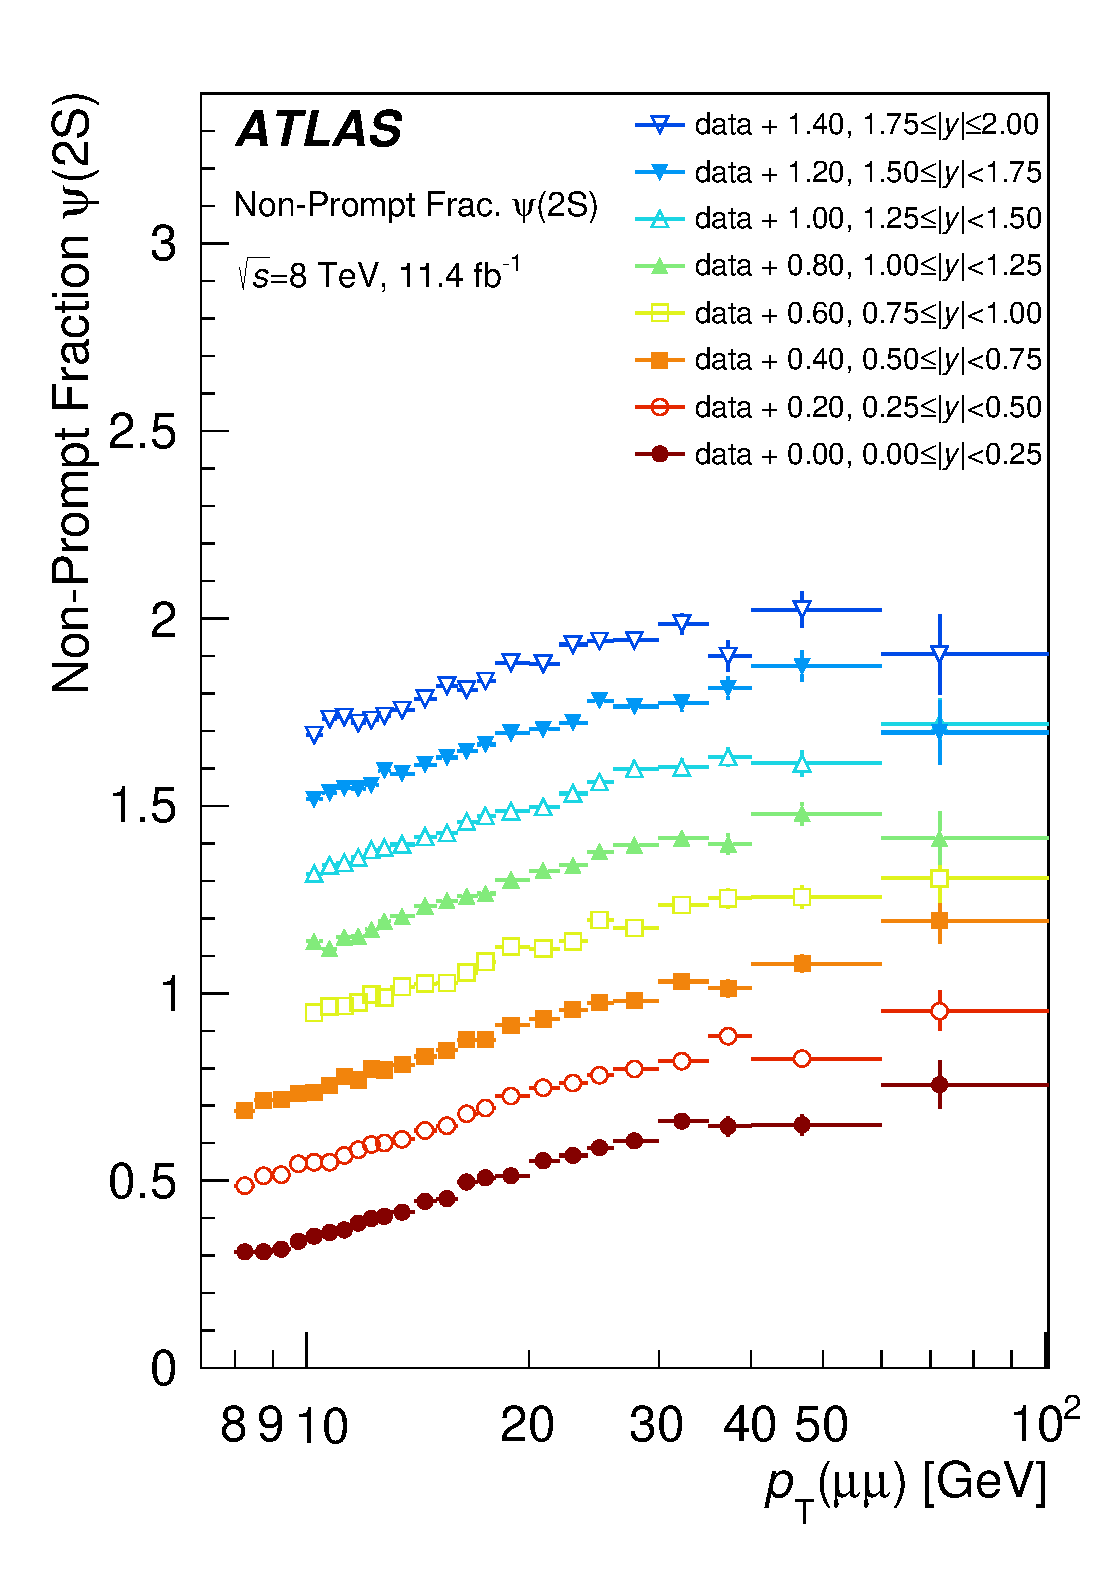
\includegraphics[width=0.44\textwidth]{figures/ct_8TeV_NPF_Psi.eps}\hfil
    \caption{The non-prompt fraction of \jpsi\ (left) and \psiprime\ (right), as a function of $\pt(\mu\mu)$ for each slice of rapidity. 
    The top (bottom) row shows the 7~\TeV\ (8~\TeV) results.
      For each increasing rapidity slice, an additional factor of 0.2 is applied to the plotted points for visual clarity. The
      centre of each bin on the horizontal axis represents the mean of the weighted $\pt$ distribution. The
      horizontal error bars represent the range of $\pt$ for the bin, and the vertical error bar covers the statistical
    and systematic  uncertainty (with the same multiplicative scaling applied).}
    \label{fig:res:NPF}
  \end{center}
\end{figure} 


\textit{Production ratios of \textmd{\psiprime} to \textmd{\jpsi} }

Figure~\ref{fig:res:PNP_Ratio} shows the ratios of \psiprime\ to \jpsi\ decaying to a muon pair in prompt and non-prompt processes,
 presented as a function of $\pt$ for slices of rapidity. The non-prompt ratio is shown to be relatively flat across the considered range of $\pT$,
for each slice of rapidity.
For the prompt ratio, a slight increase as a function of $\pt$ is observed, with no strong dependence on rapidity or centre-of-mass energy.

\begin{figure} [!ht]
  \begin{center}
    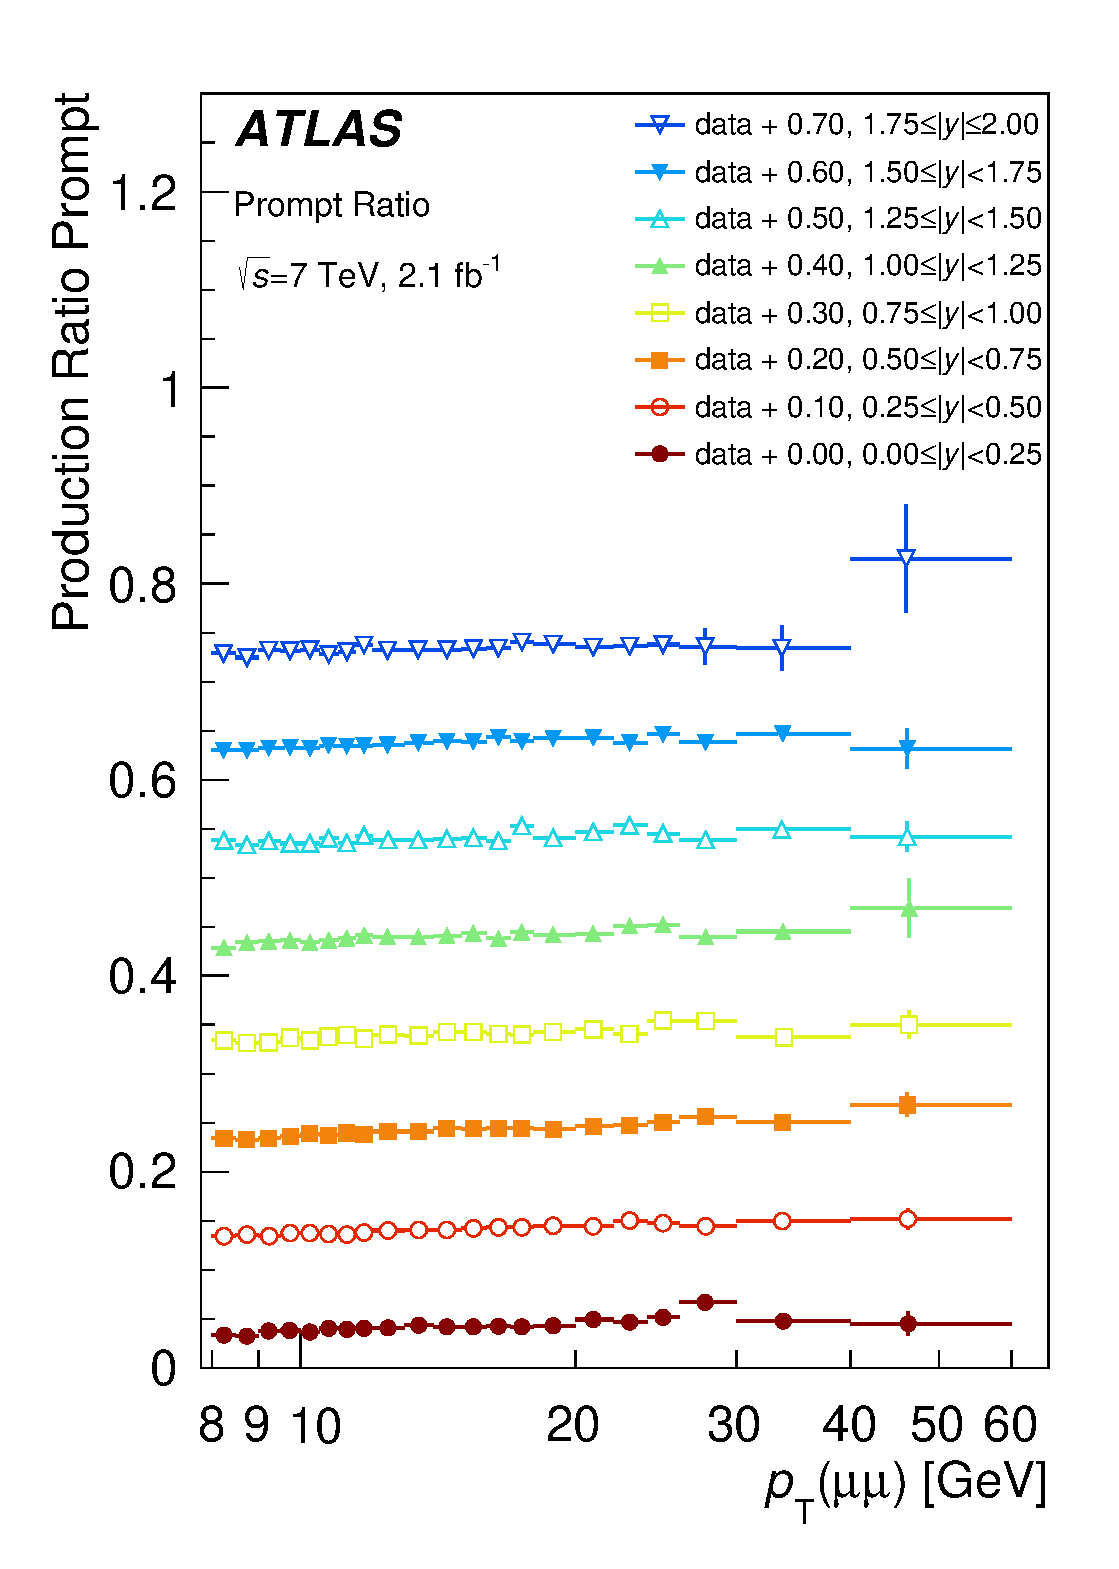
\includegraphics[width=0.44\textwidth]{figures/ct_7TeV_P_Ratio.eps} 
    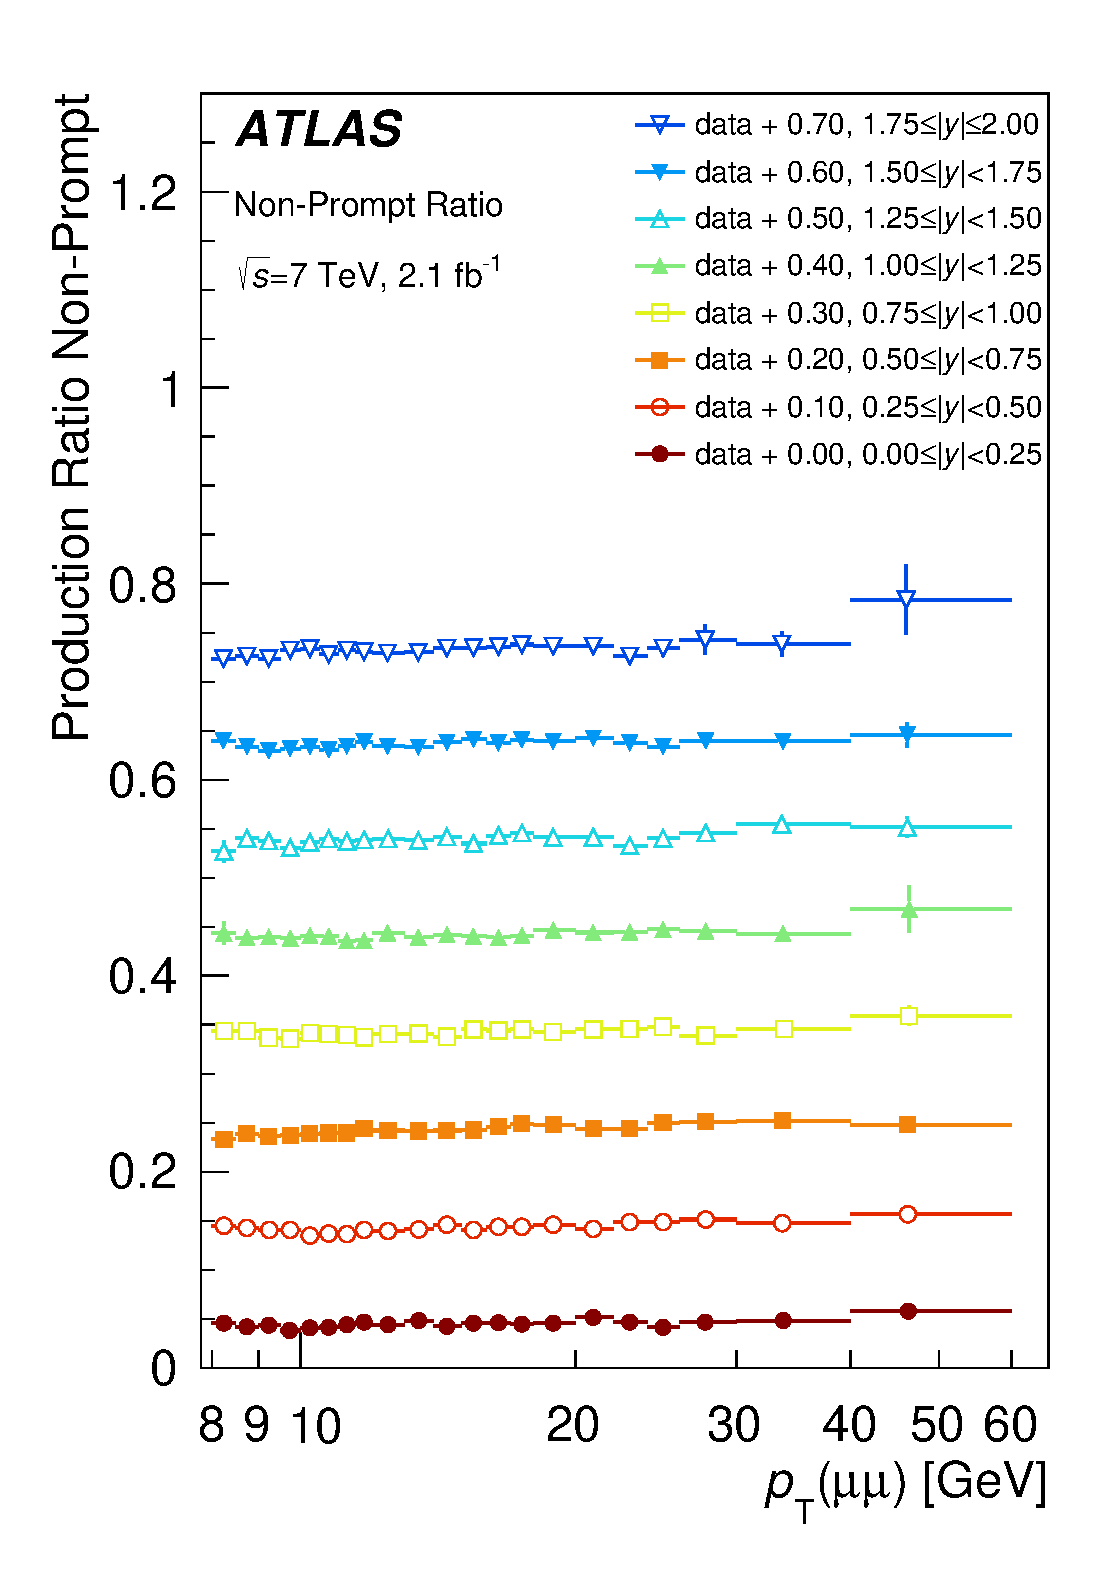
\includegraphics[width=0.44\textwidth]{figures/ct_7TeV_NP_Ratio.eps}\hfil\\
    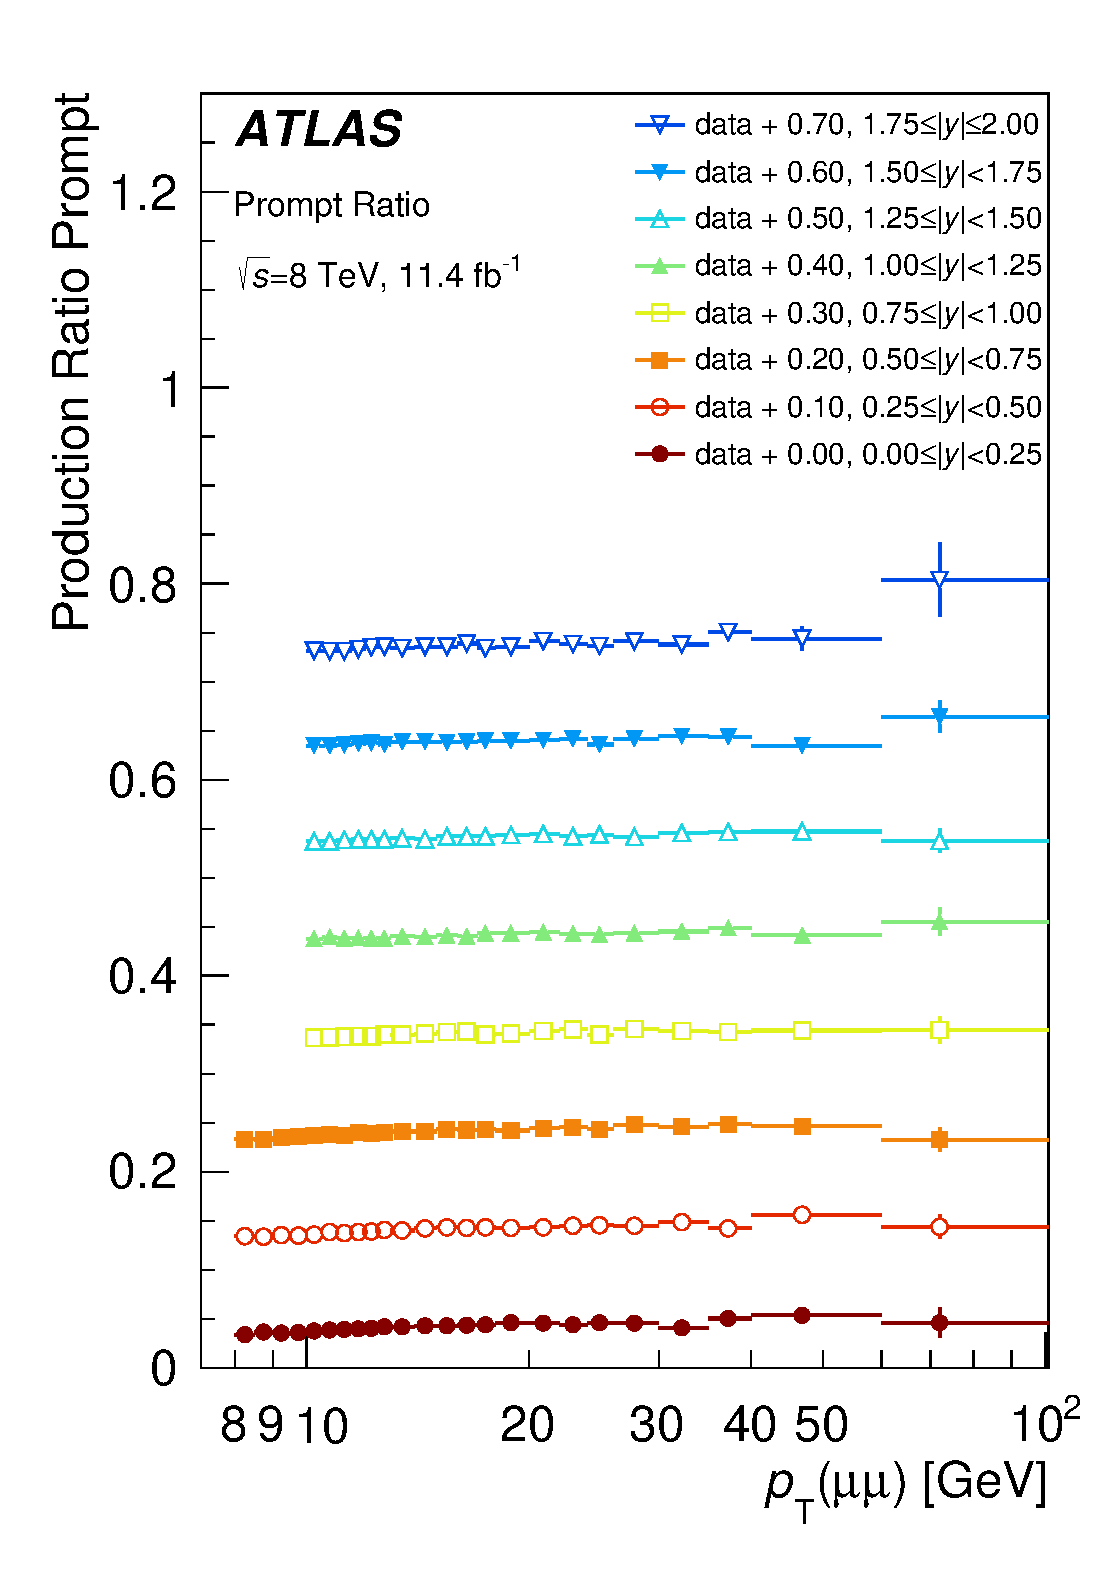
\includegraphics[width=0.44\textwidth]{figures/ct_8TeV_P_Ratio.eps}
    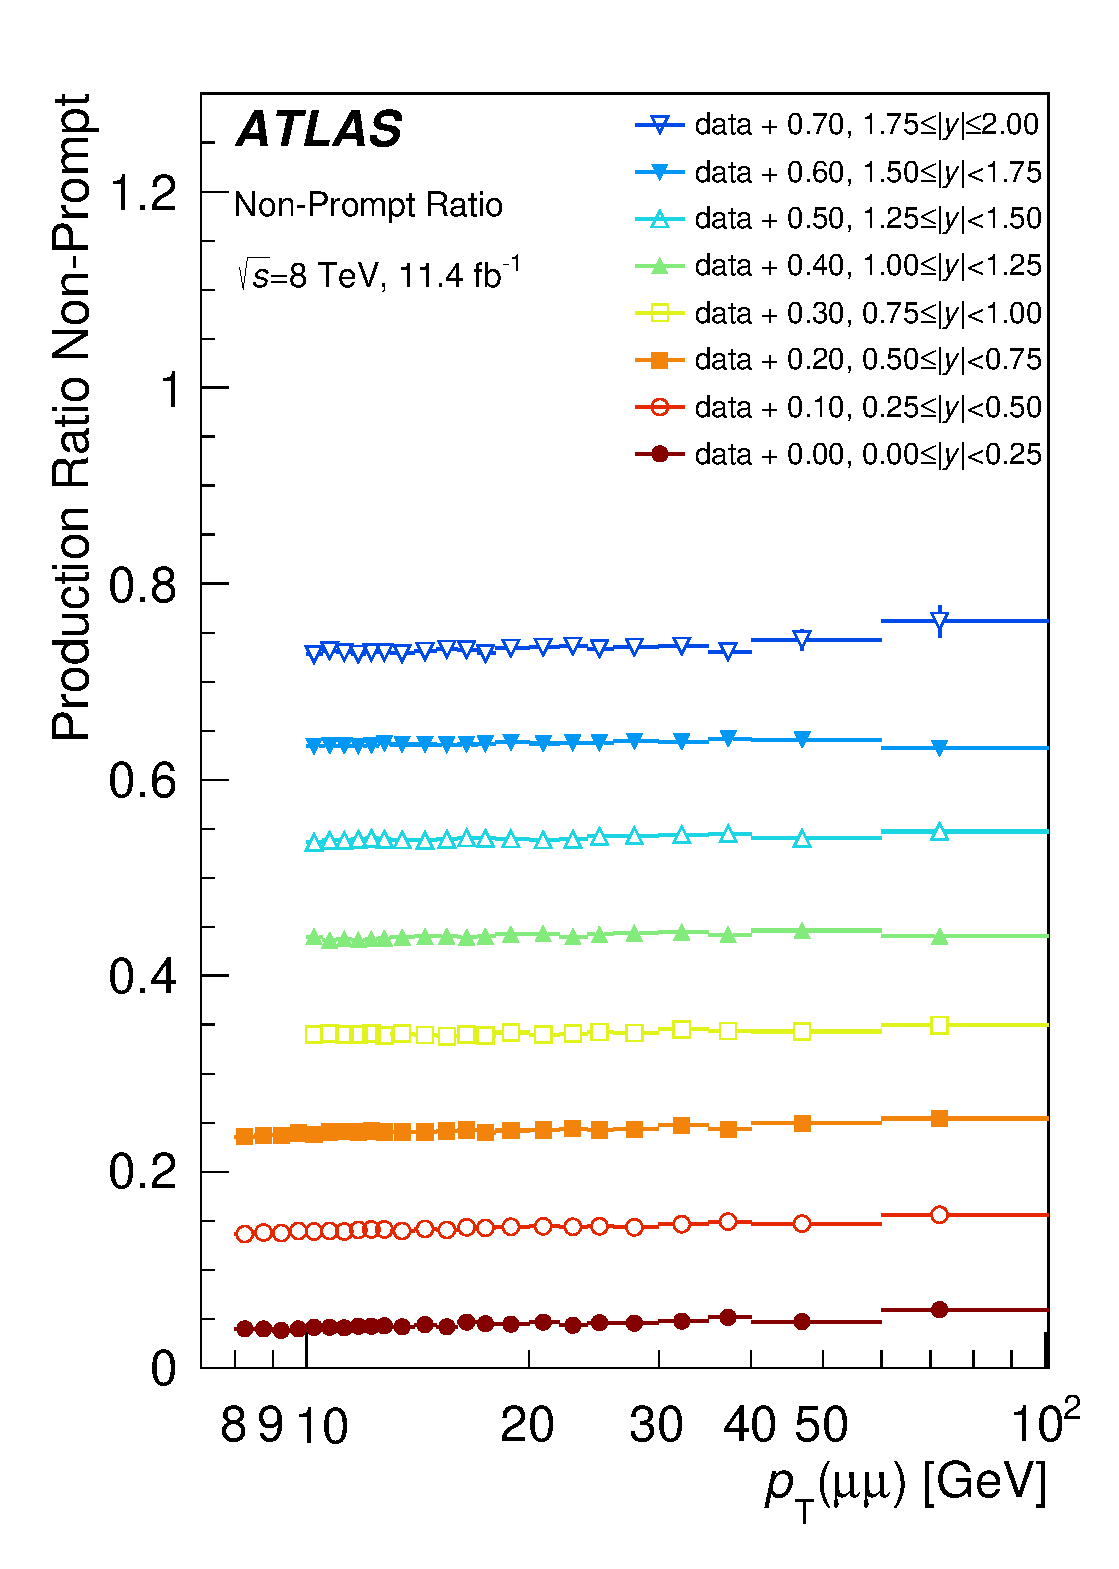
\includegraphics[width=0.44\textwidth]{figures/ct_8TeV_NP_Ratio.eps}\hfil
    \caption{The ratio of \psiprime\ to \jpsi\ production times dimuon branching fraction for prompt (left) and non-prompt (right) processes
    as a function of $\pt(\mu\mu)$  for each of the slices of rapidity. 
    For each increasing rapidity slice, an additional factor of 0.1 is applied to the plotted points for visual clarity.
    The top (bottom) row shows the 7~\TeV\ (8~\TeV) results.
      The centre of each bin on the horizontal axis represents the mean of the weighted $\pt$ distribution. The
      horizontal error bars represent the range of $\pt$ for the bin, and the vertical error bar covers the statistical and systematic uncertainty.}
    \label{fig:res:PNP_Ratio}
  \end{center}
\end{figure} 

\clearpage


\item[Comparison with theory] \hfill \\
For prompt production, as shown in Figure~\ref{fig:xsecPtheoryRatio}, the ratio of the NLO NRQCD theory calculations~\cite{Shao:2012iz} 
to data is provided for \Jpsi\ and \psiprime\ at both the 7 and 8~\TeV\ centre-of-mass energies.
The theory predictions are 
based on the long-distance matrix elements (LDMEs) from Refs.~\cite{NRQCD1,Ma:2010vd}, with uncertainties originating from the
choice of scale, charm quark mass and LDMEs (see Refs.~\cite{Shao:2012iz,Kanaki:2000ey,NRQCD1,Ma:2010vd} for more details).
Figure~\ref{fig:xsecPtheoryRatio} shows fair agreement between the theoretical calculation and the data points for the whole $\pt$ range. 
The ratio of theory to data does not depend on rapidity.

\begin{figure} [!ht]
  \begin{center}
    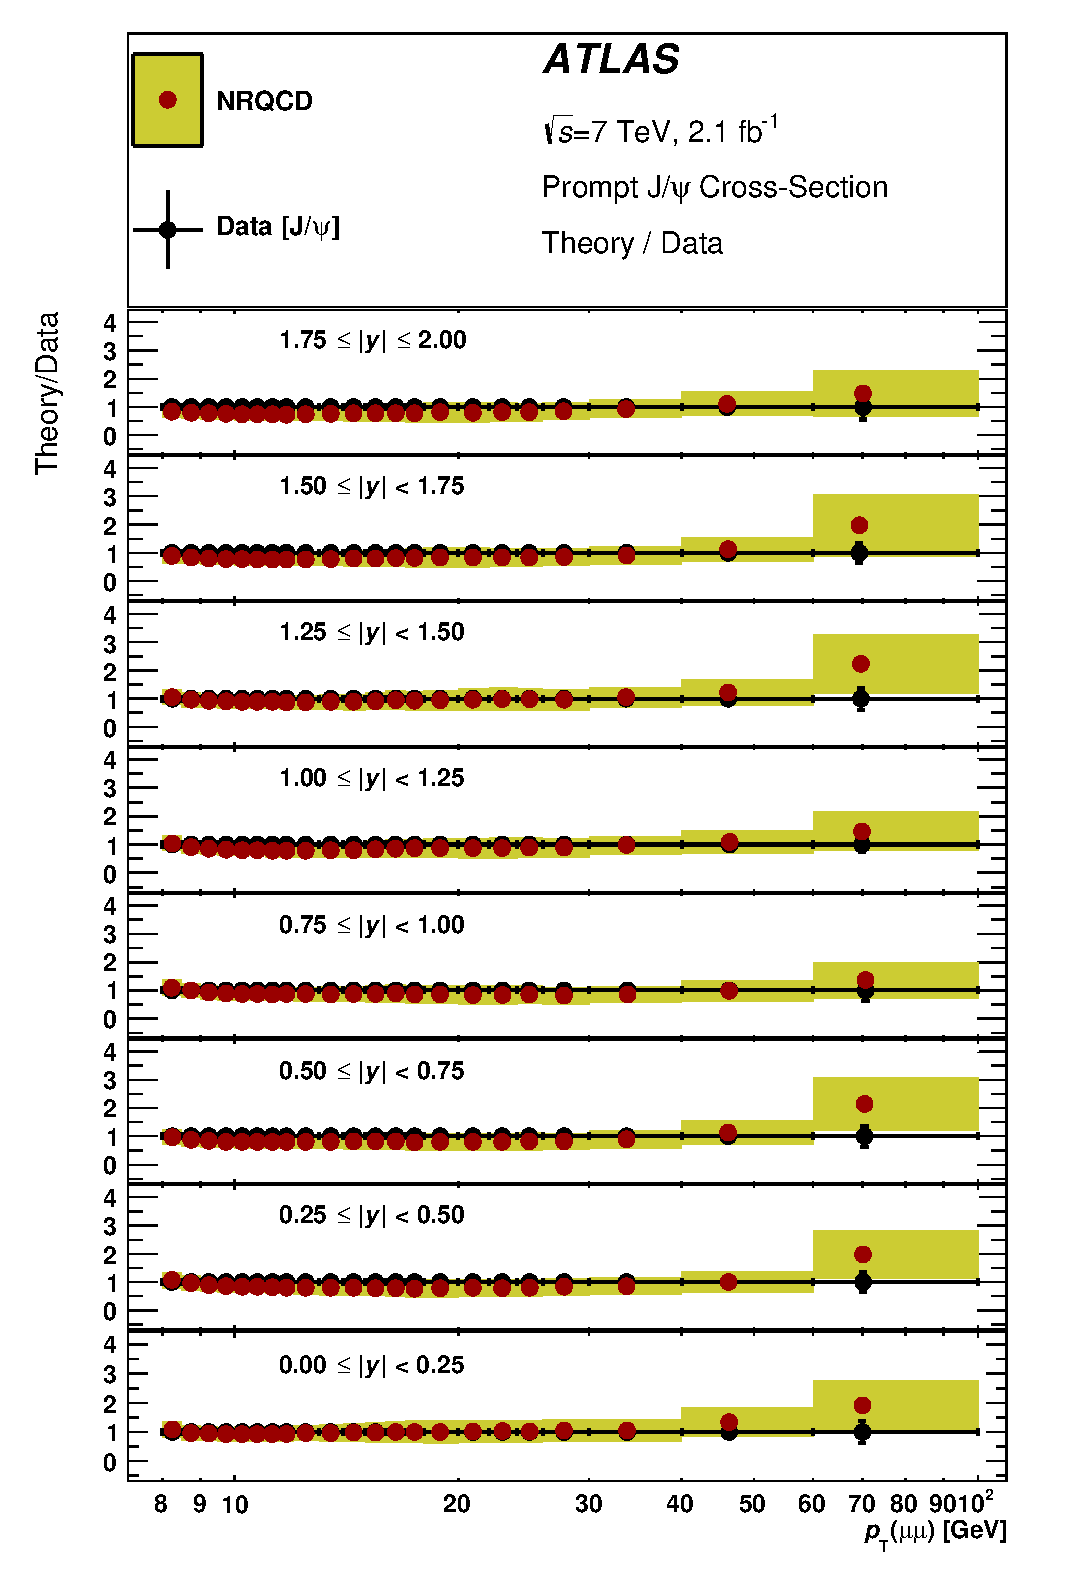
\includegraphics[width=0.44\textwidth]{figures/ct_7TeV_JpsiP_theoryRatio_lin.eps} 
    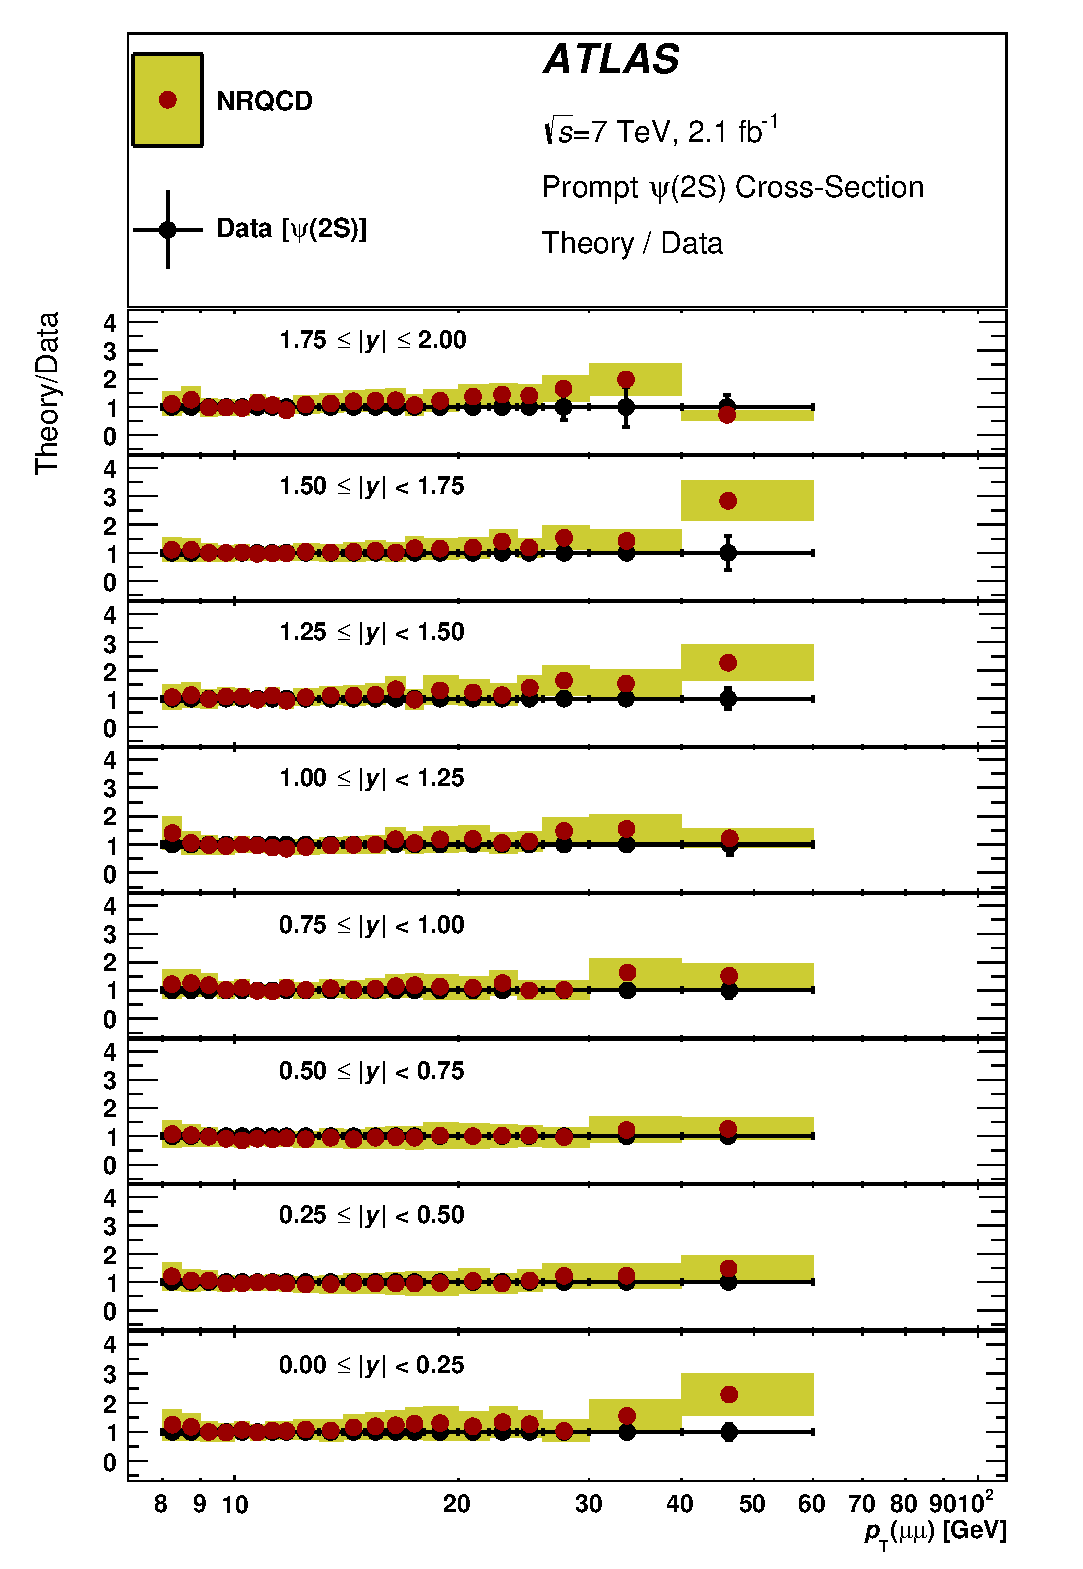
\includegraphics[width=0.44\textwidth]{figures/ct_7TeV_Psi2SP_theoryRatio_lin.eps}\hfil\\
    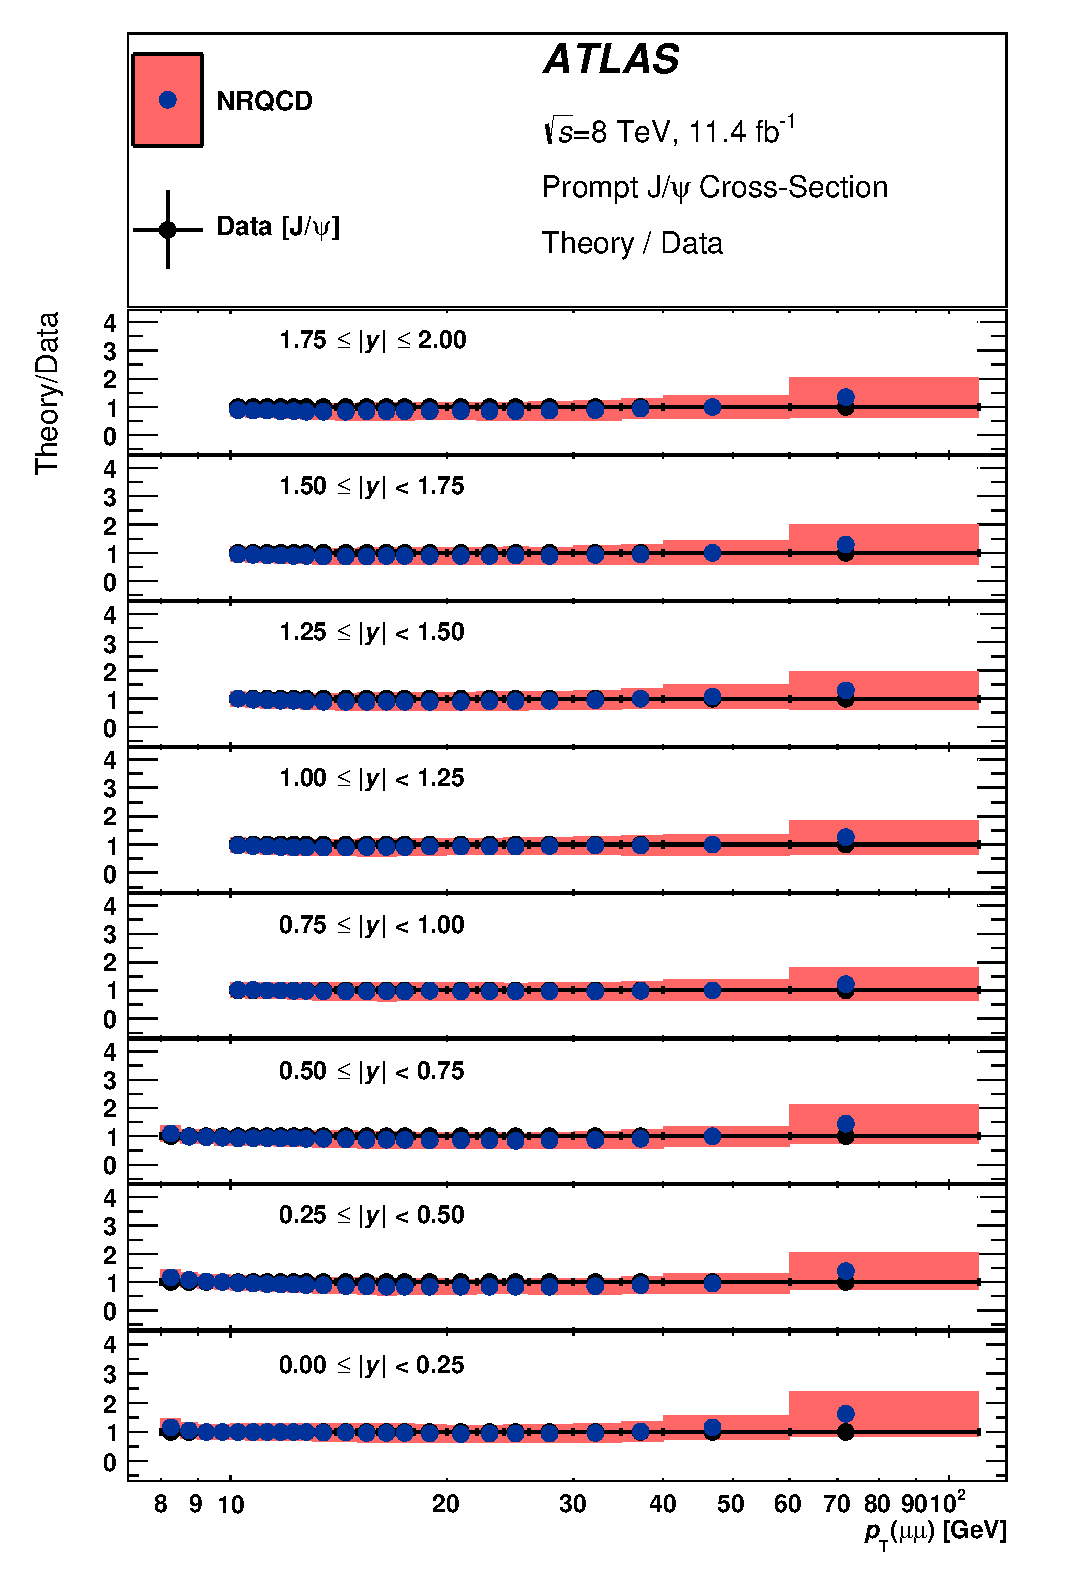
\includegraphics[width=0.44\textwidth]{figures/ct_8TeV_JpsiP_theoryRatio_lin.eps}
    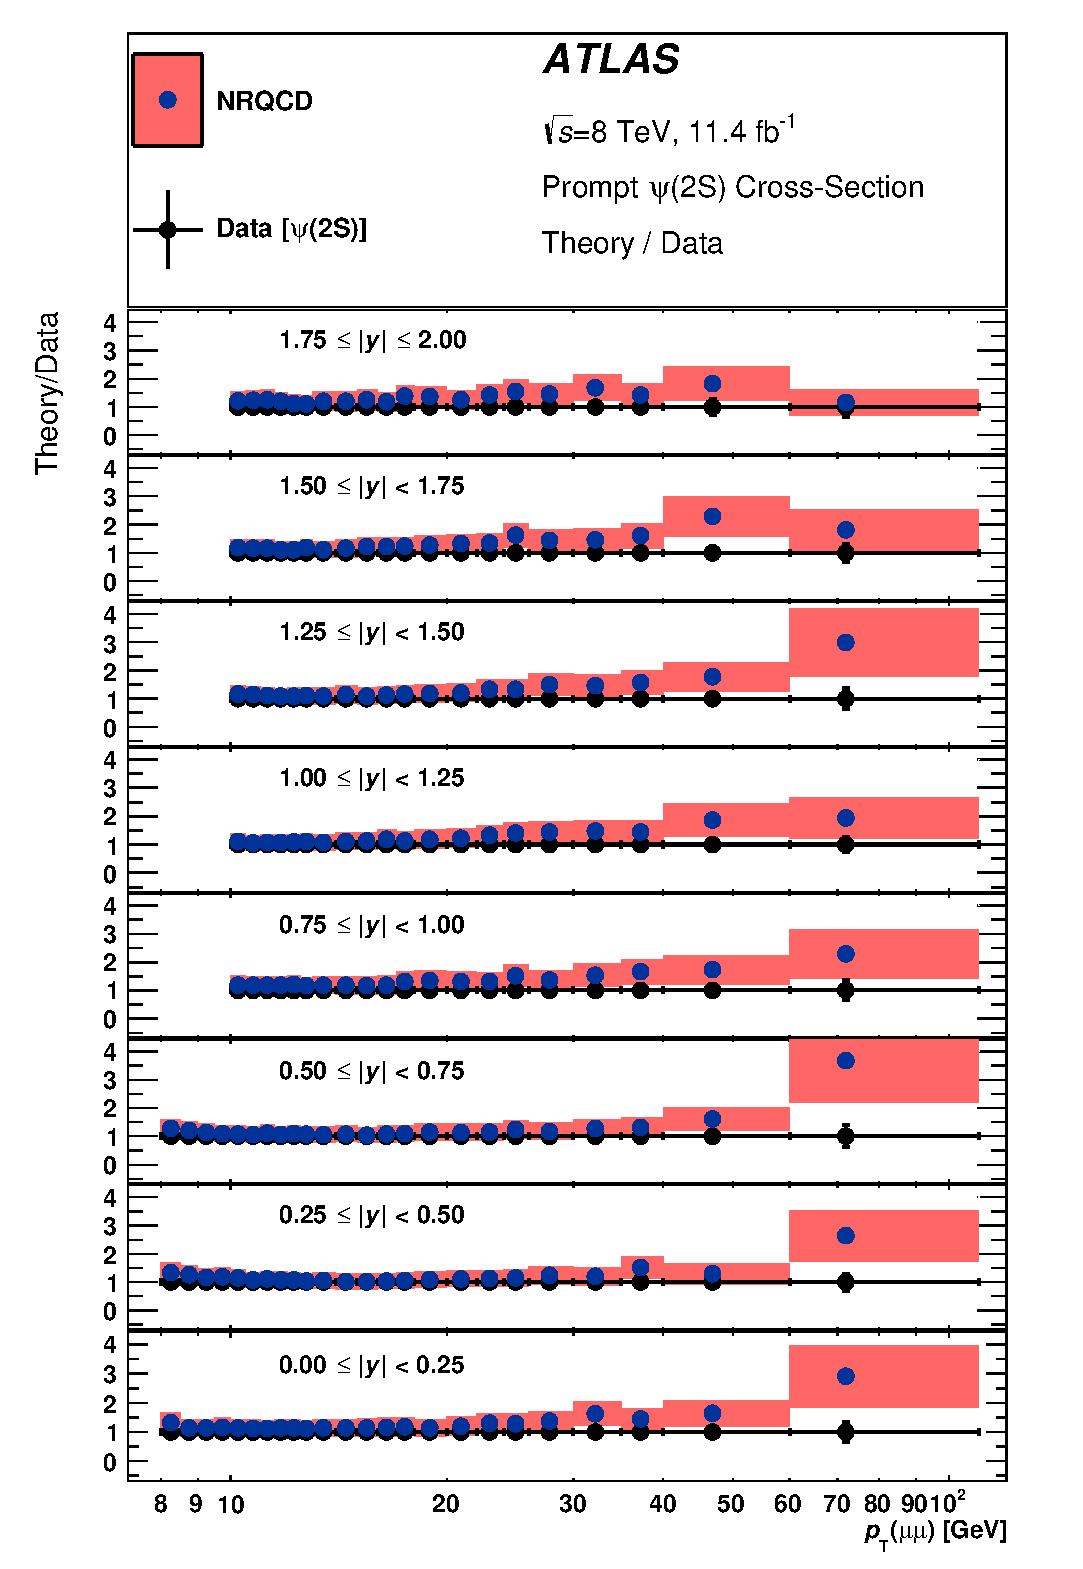
\includegraphics[width=0.44\textwidth]{figures/ct_8TeV_Psi2SP_theoryRatio_lin.eps}\hfil
    \caption{The ratios of the NRQCD theoretical predictions to data are presented for the differential prompt cross-section of \jpsi\ (left) and \psiprime\ (right) as a function 
    of $\pt(\mu\mu)$ for each rapidity slice. 
    The top (bottom) row shows the 7~\TeV\ (8~\TeV) results.
    The error on the data is the relative error of each data point, while the error bars on the theory prediction are the relative error of each theory point.}
    \label{fig:xsecPtheoryRatio}
  \end{center}
\end{figure} 

For non-prompt $\psi$ production, comparisons are made to FONLL theoretical predictions~\cite{FONLL_2001,Cacciari:2012ny}, which describe the production of 
$b$-hadrons followed by their decay into $\psi+X$.
Figure~\ref{fig:xsecNPtheoryRatio} shows the ratios of $\jpsi$ and $\psiprime$ FONLL predictions to data, as a function of $\pt$ and in slices of rapidity, 
for centre-of-mass energies of~7 and 8~\TeV.
For $\jpsi$, agreement is generally good, but the theory predicts slightly harder $\pt$ spectra than observed in the data.
For $\psiprime$, the shapes of data and theory appear to be in satisfactory agreement, but the theory predicts higher yields than in the data.
There is no observed dependence on rapidity in the comparisons between theory and data for non-prompt \jpsi\ and \psiprime\ production.


\begin{figure} [!ht]
  \begin{center}
    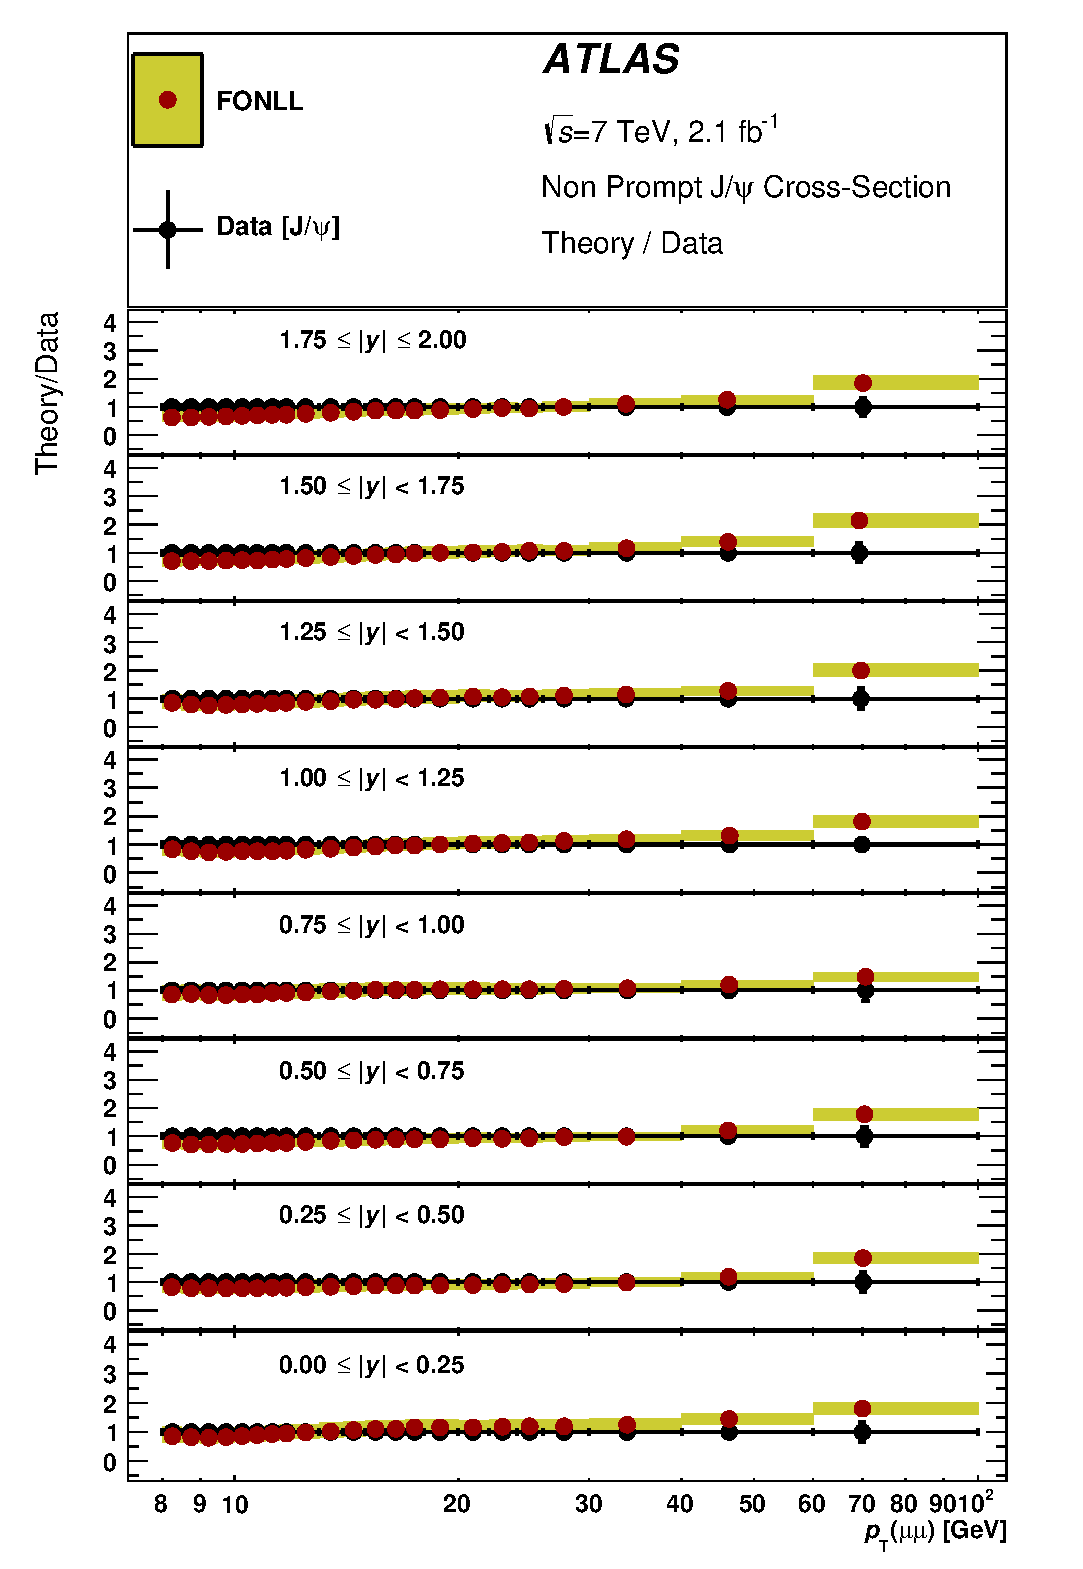
\includegraphics[width=0.44\textwidth]{figures/ct_7TeV_JpsiNP_theoryRatio_lin.eps} 
    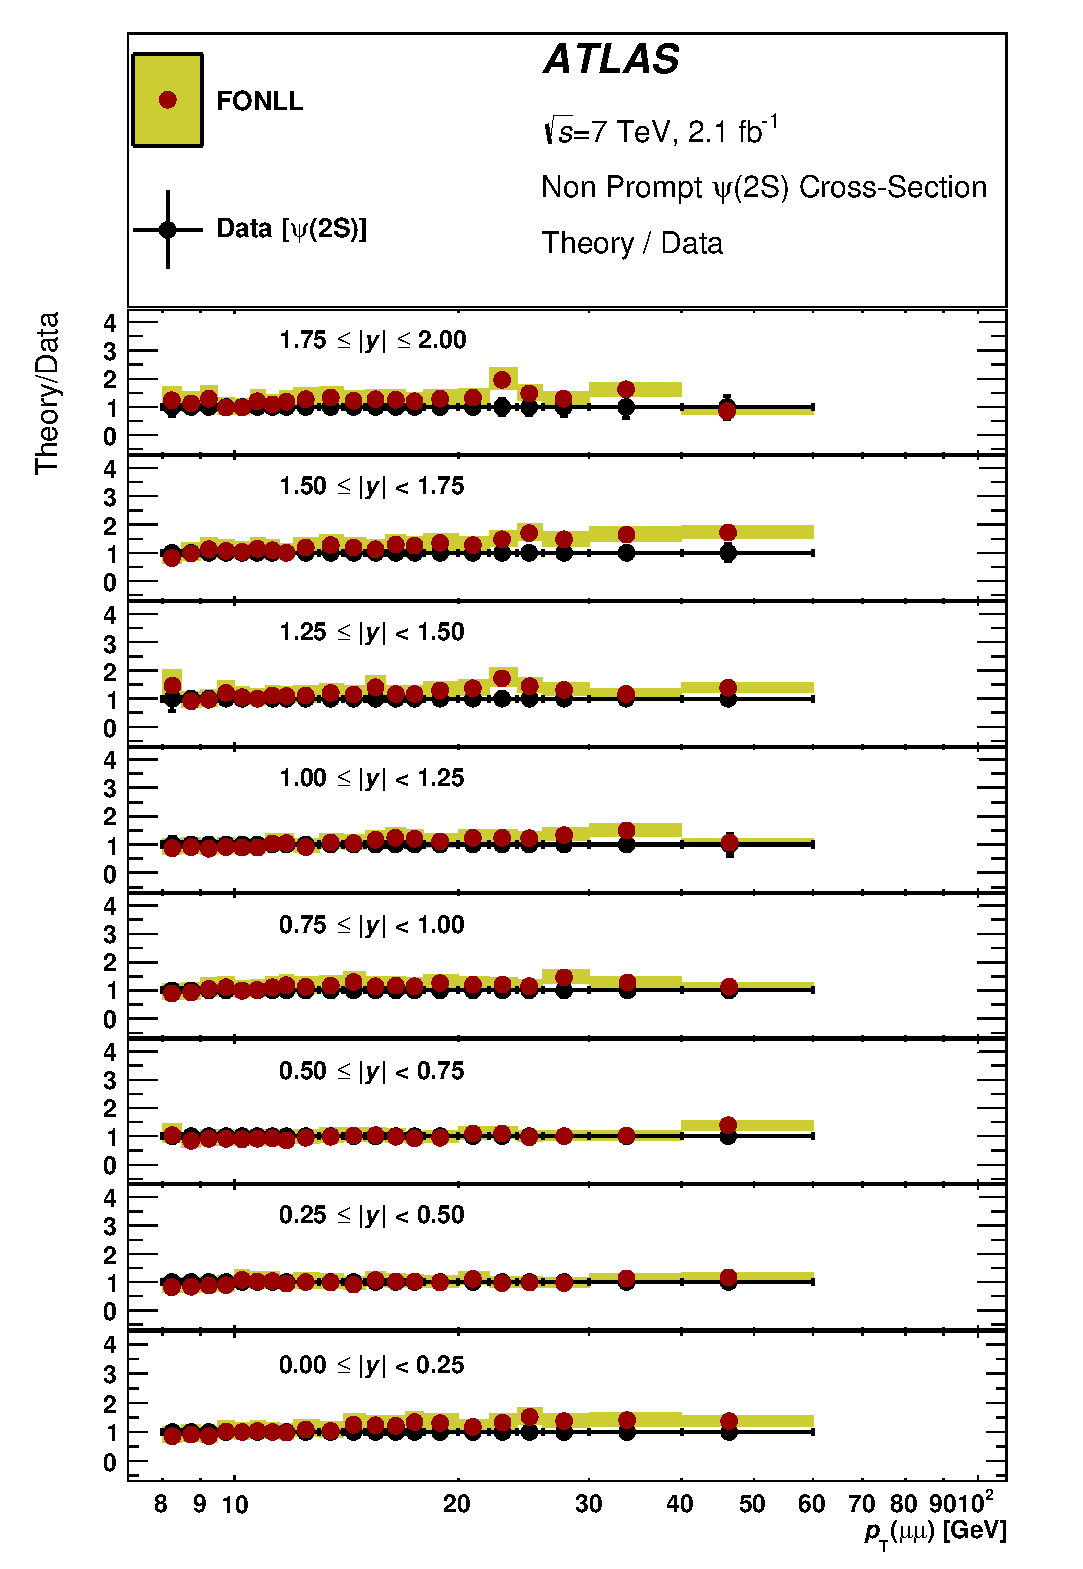
\includegraphics[width=0.44\textwidth]{figures/ct_7TeV_Psi2SNP_theoryRatio_lin.eps}\hfil\\
    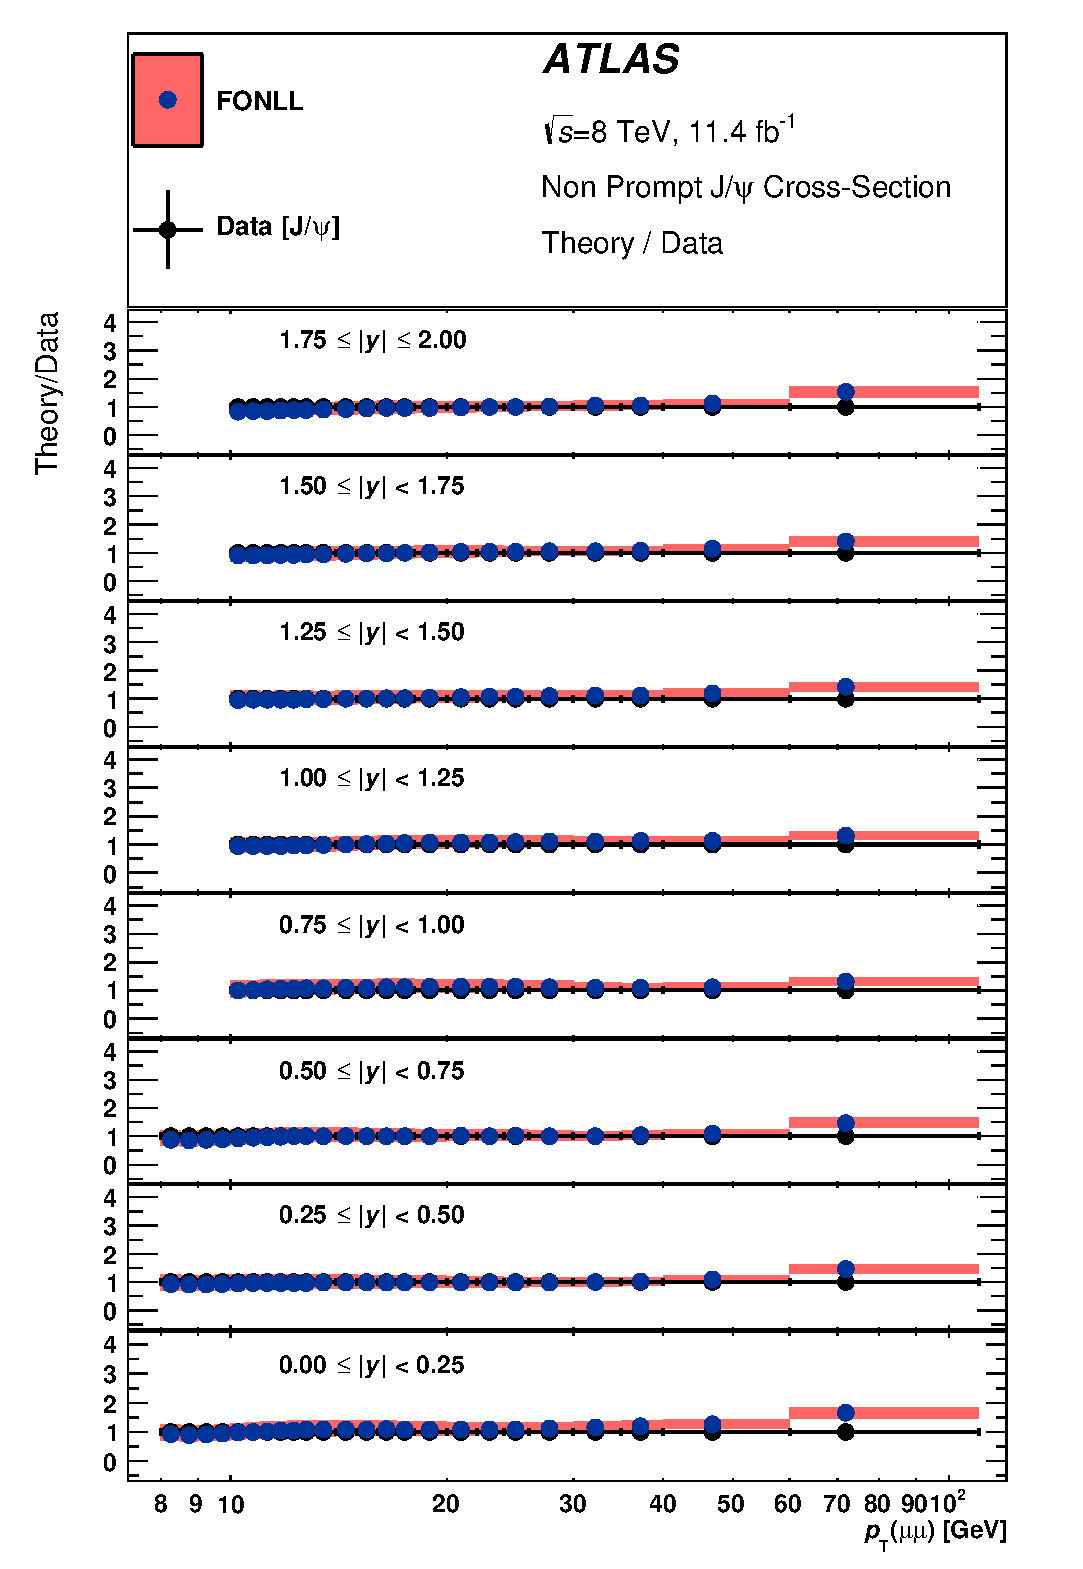
\includegraphics[width=0.44\textwidth]{figures/ct_8TeV_JpsiNP_theoryRatio_lin.eps}
    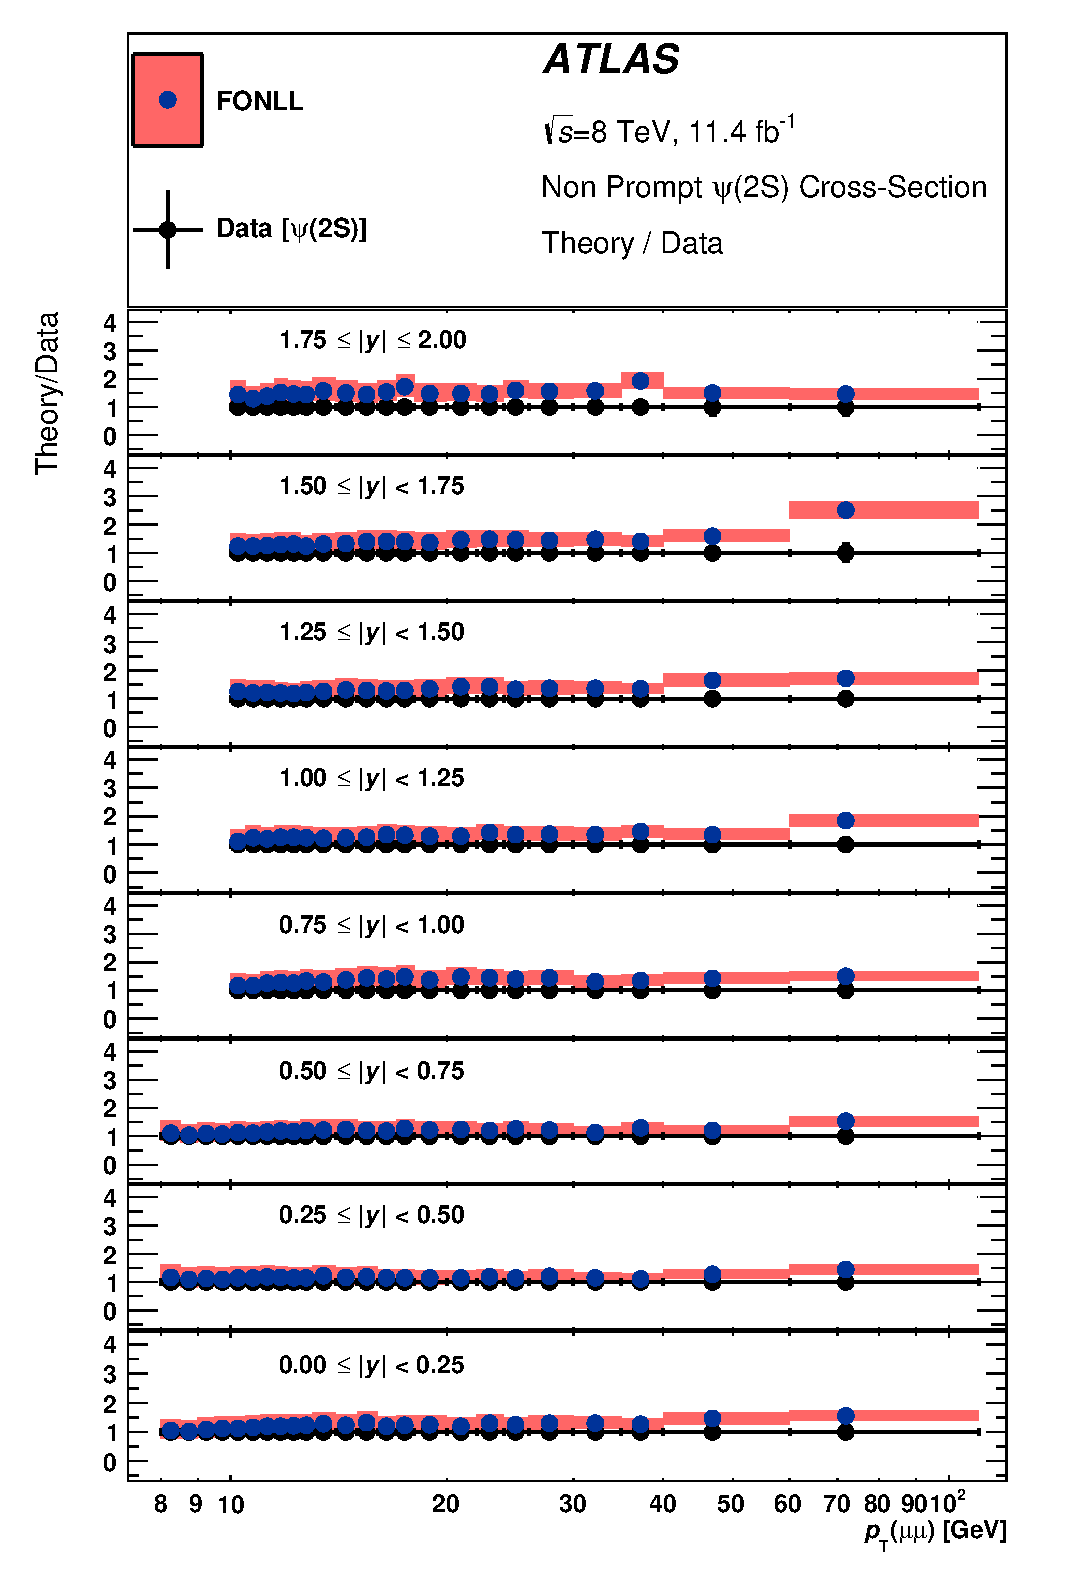
\includegraphics[width=0.44\textwidth]{figures/ct_8TeV_Psi2SNP_theoryRatio_lin.eps}\hfil
    \caption{The ratio of the FONLL theoretical predictions to data are presented for the differential non-prompt 
    cross-section of \jpsi\ (left) and \psiprime\ (right) as a function 
    of $\pt(\mu\mu)$ for each rapidity slice. 
    The top (bottom) row shows the 7~\TeV\ (8~\TeV) results.
    The error on the data is the relative error of each data point, while the error bars on the theory prediction are the relative error of each theory point.}
    \label{fig:xsecNPtheoryRatio}
  \end{center}
\end{figure} 


\item[Comparison of cross-sections 8~\TeV\  with 7~\TeV\ ] \hfill \\

It is interesting to compare the cross-section results between the two centre-of-mass energies, for both data and the theoretical predictions.

Figure~\ref{fig:xsecEnergyRatio} shows the 8~\TeV\  to 7~\TeV\  cross-section ratios of prompt and non-prompt $\jpsi$ and $\psiprime$ for both data sets.
For the theoretical ratios the uncertainties are neglected here, since the high correlation between them results in large cancellations.


Due to a finer granularity in $\pt$ for the 8~\TeV\  data, a weighted average of the 8~\TeV\ results is taken across equivalent intervals of the 7~\TeV\ data to enable direct comparisons.
Both data and theoretical predictions agree 
that the ratios become larger with increasing $\pt$,
however at the lower edge of the $\pT$ range the data tends to be slightly below theory.


\begin{figure} [!ht]
  \begin{center}
    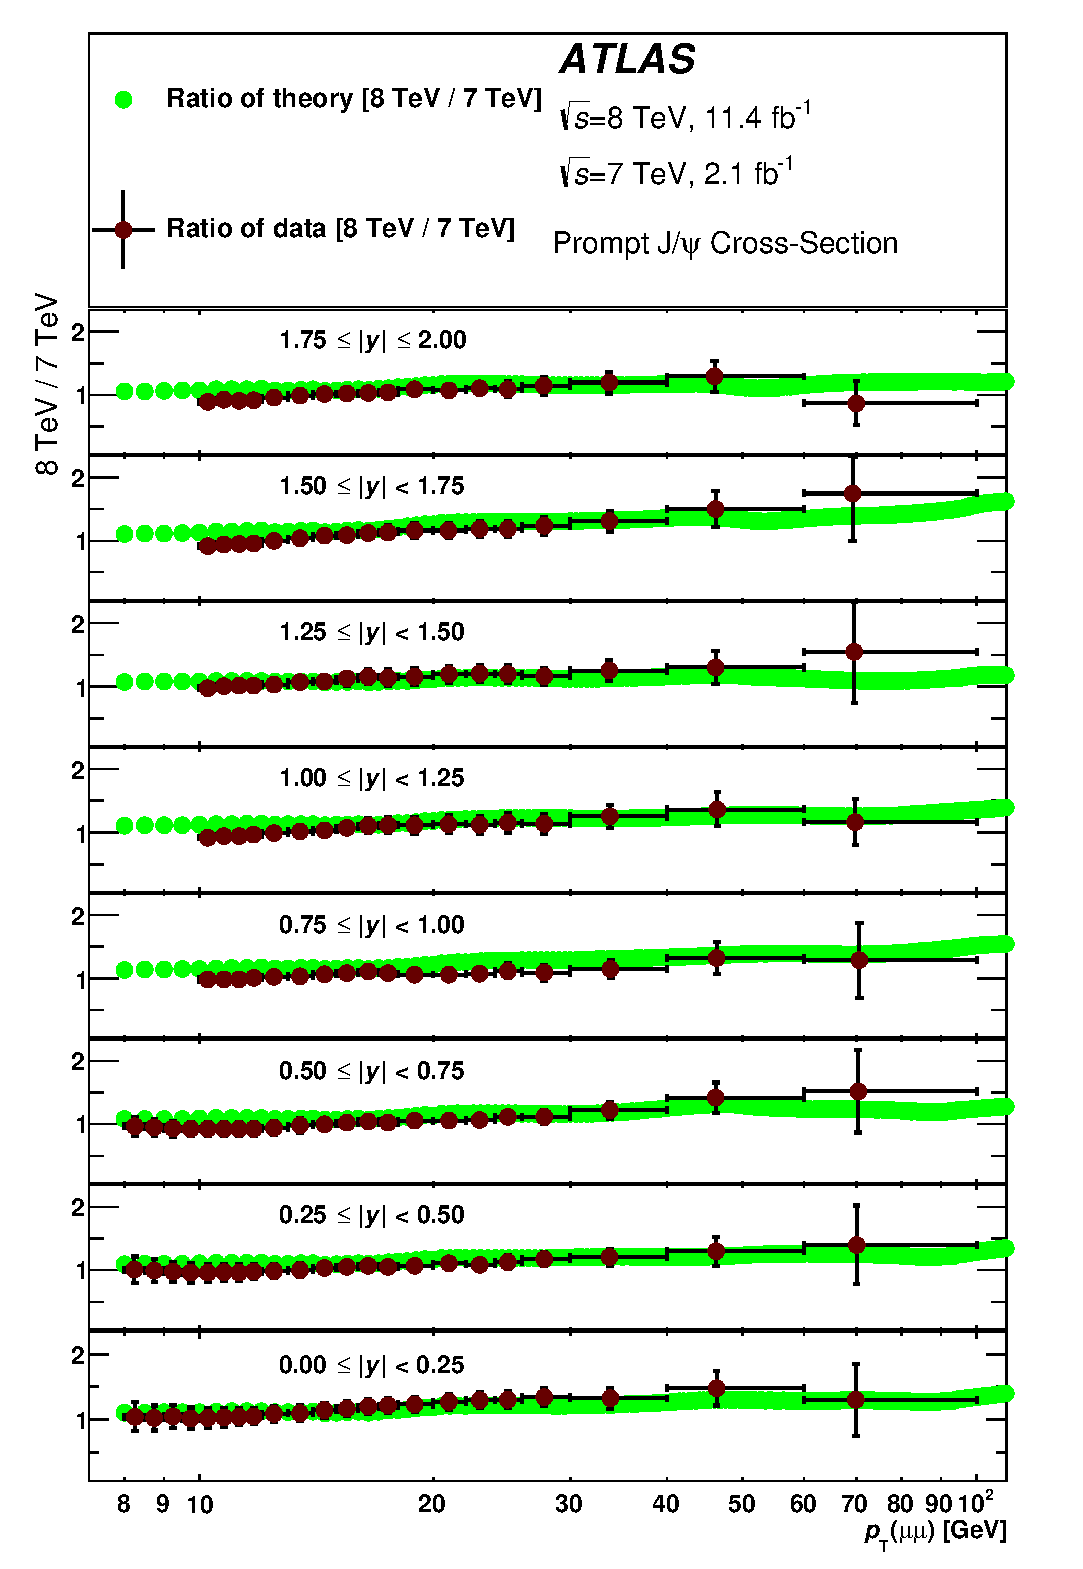
\includegraphics[width=0.44\textwidth]{figures/rt_th_xSecP_J.eps} 
    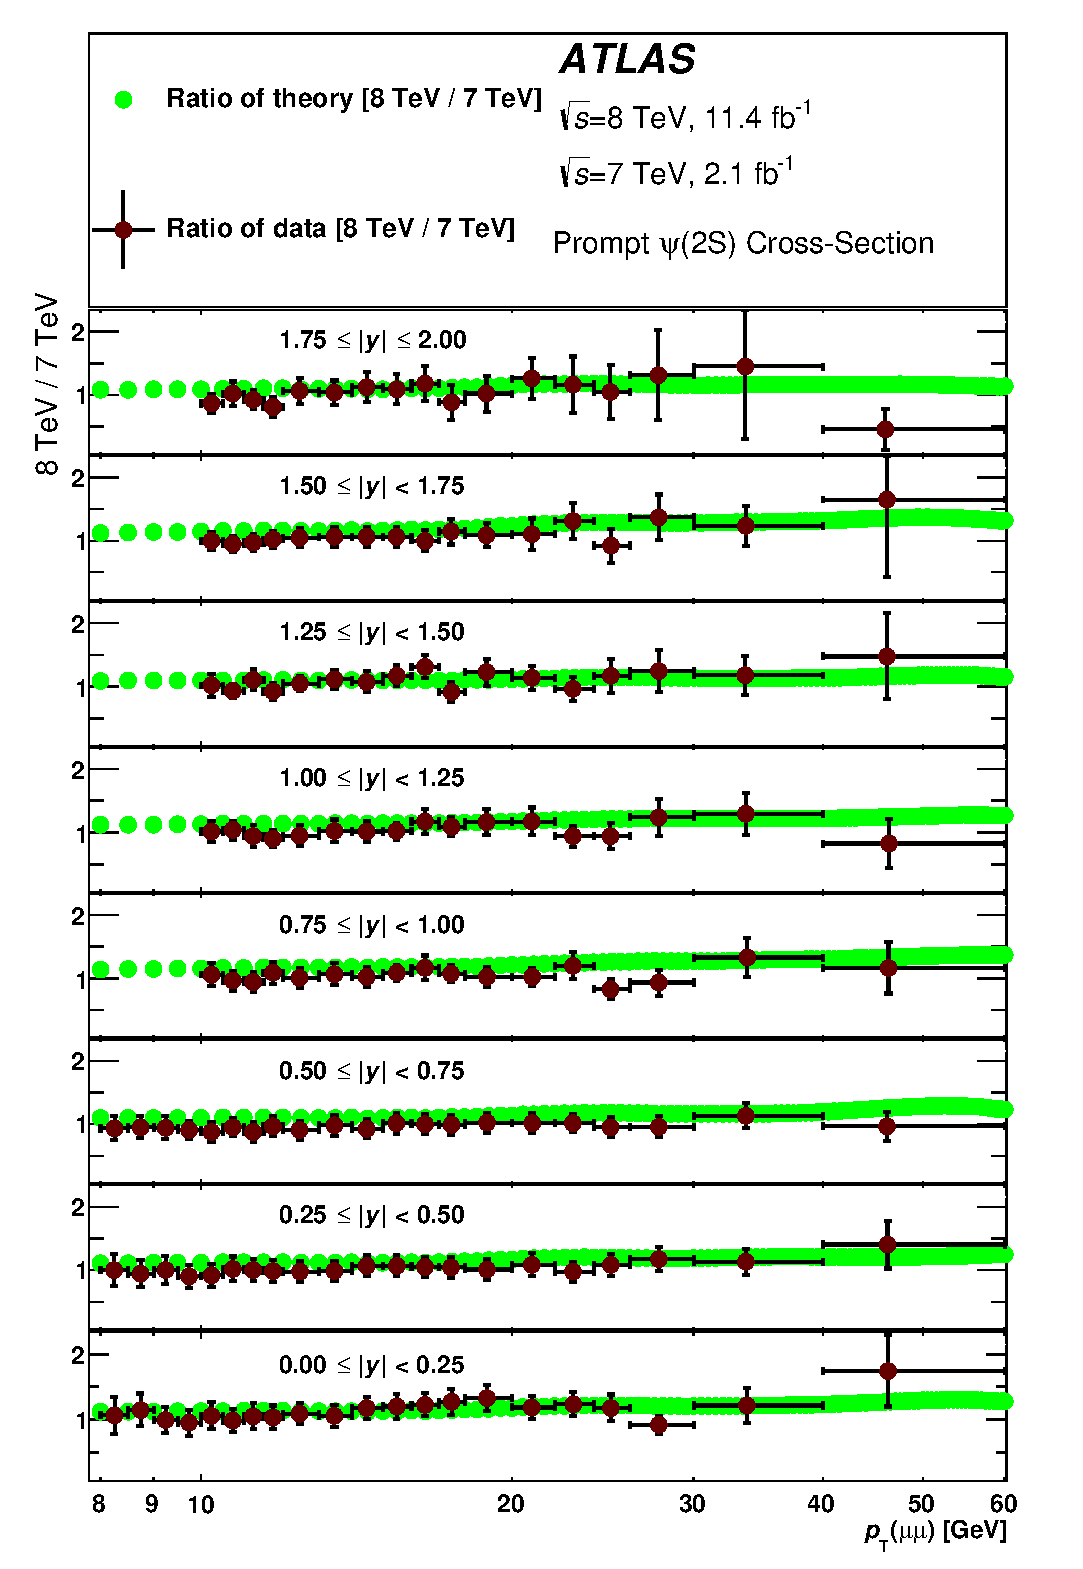
\includegraphics[width=0.44\textwidth]{figures/rt_th_xSecP_P.eps}\hfil\\
    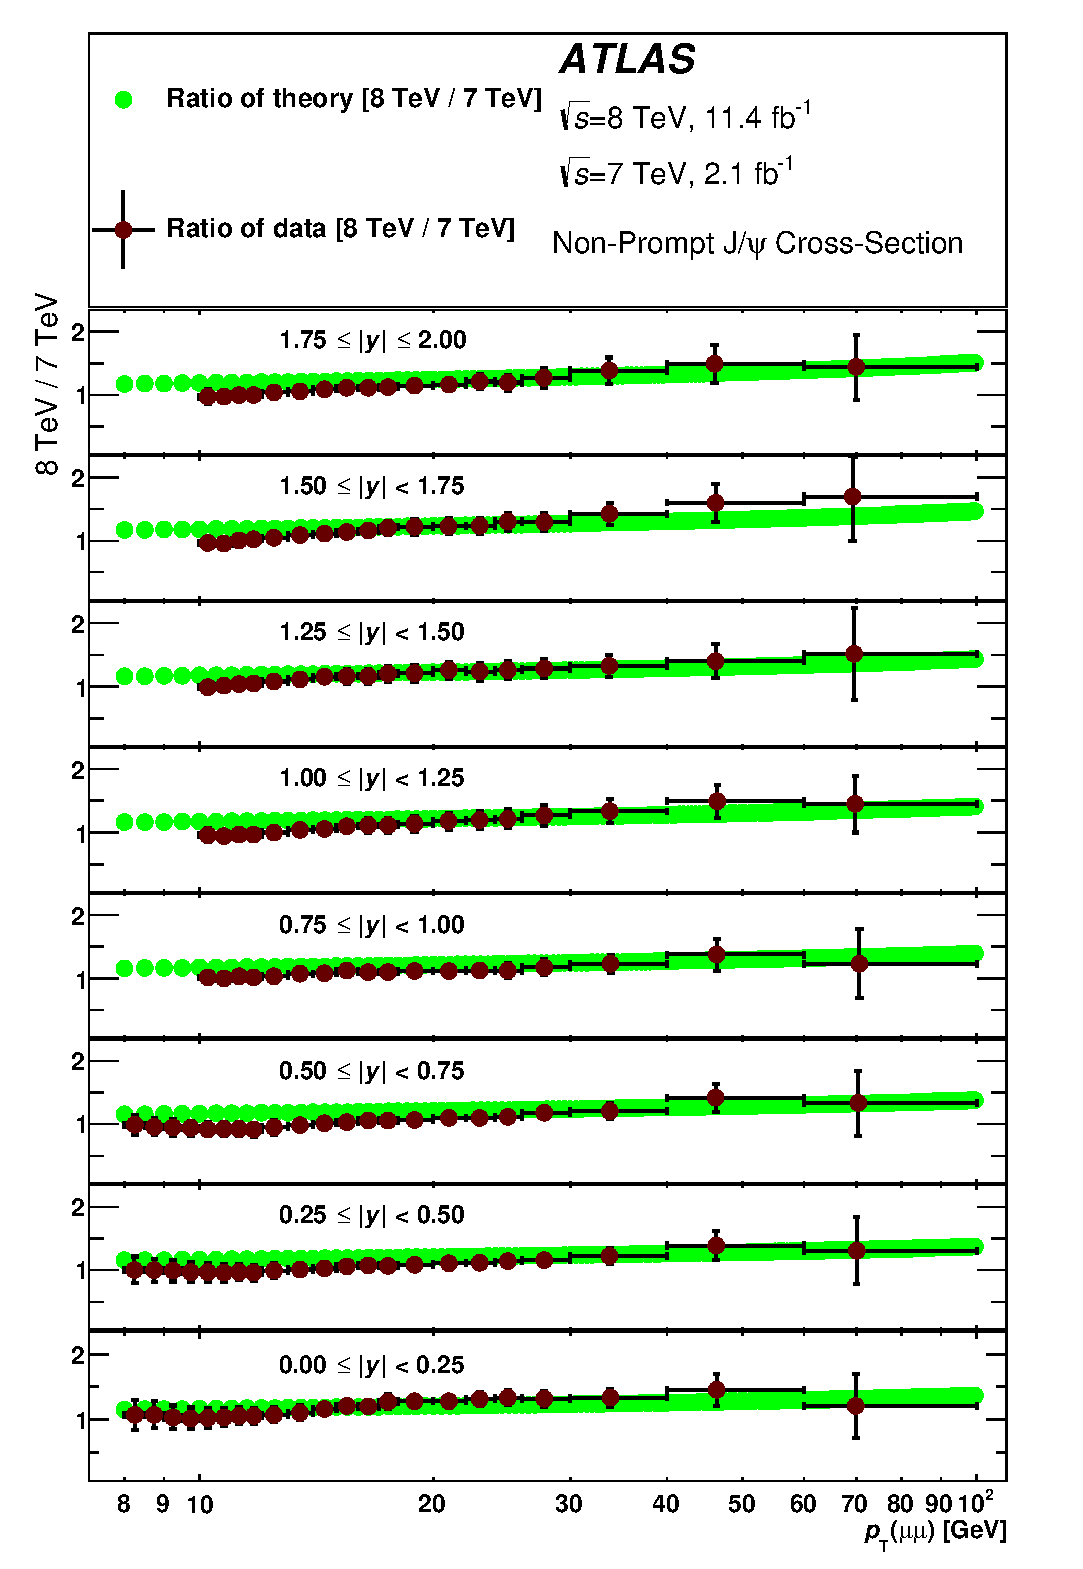
\includegraphics[width=0.44\textwidth]{figures/rt_th_xSecNP_J.eps}
    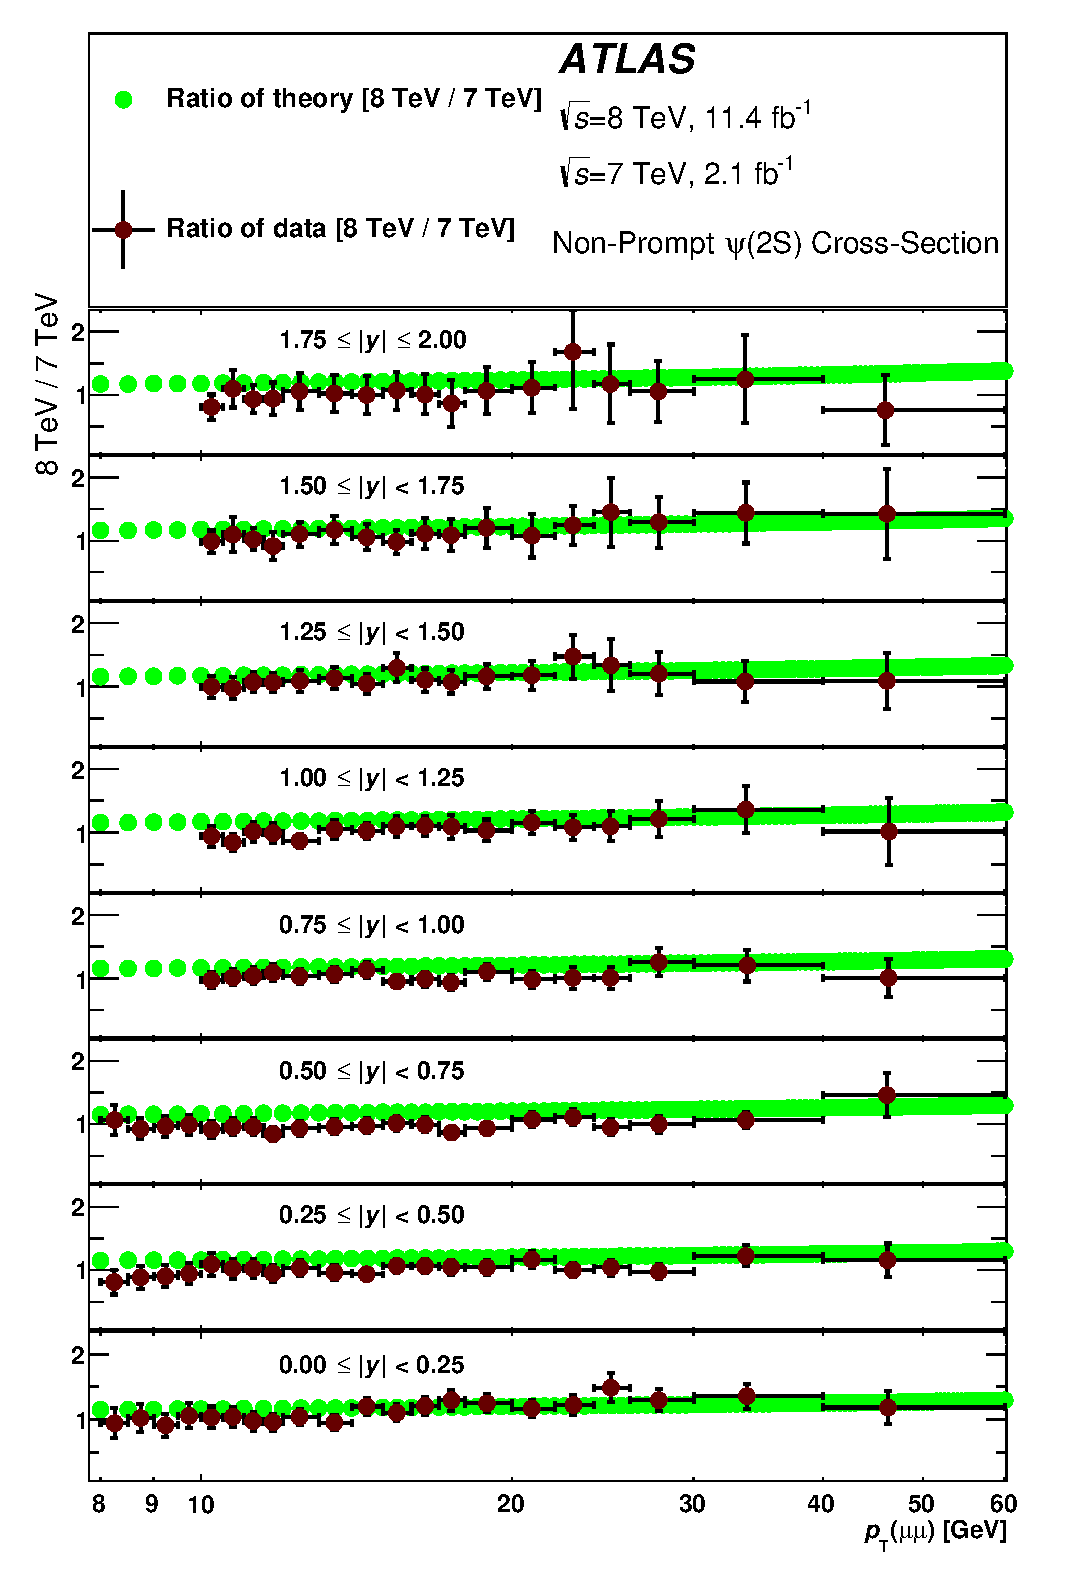
\includegraphics[width=0.44\textwidth]{figures/rt_th_xSecNP_P.eps}\hfil
    \caption{The ratio of the 8~\TeV\ and 7~\TeV\ differential cross-sections
	    are presented for prompt~(top) and non-prompt~(bottom) $\jpsi$~(left) and 
	    $\psiprime$~(right) for both data~(red points with error bars) and theoretical predictions~(green points).
	    The theoretical predictions used are NRQCD for prompt and FONLL for non-prompt production.
	    The uncertainty on the data ratio does not account for possible correlations between 7 and 8 \TeV\  data, and no uncertainty is shown 
	    for the ratio of theory predictions.
}
    \label{fig:xsecEnergyRatio}
  \end{center}
\end{figure} 


\end{description}


\FloatBarrier


\section{Conclusion}
\label{sec:conclusion}

The prompt and non-prompt production cross-sections, the non-prompt production fraction of the $\jpsi$ and $\psiprime$
decaying into two muons, the ratio of prompt $\psiprime$ to prompt $\jpsi$ production, and the ratio of non-prompt $\psiprime$ to non-prompt $\jpsi$ production
were measured in the rapidity range
$|y|<2.0$ for transverse momenta between $8$ and $110$~\GeV. This measurement was carried out using \lumiA (\lumiB) of $pp$
collision data at a centre-of-mass energy of $7$ \TeV\ ($8$ \TeV) recorded by the ATLAS experiment at the LHC. It is the latest in a series of 
related measurements of the production of charmonium states
made by ATLAS.
In line with previous measurements, the central values were obtained 
assuming isotropic $\psi \to \mu\mu$ decays.
Correction factors for these cross-sections, computed for a number of extreme spin-alignment scenarios, are between $-35\%$ and $+100\%$ at the lowest transverse momenta studied, and between $-14\%$ and $+9\%$ at the highest transverse momenta, depending on the specific scenario.

The ATLAS measurements presented here extend the range of existing measurements to higher transverse momenta, and to a higher collision energy of $\sqrt{s} = 8$ \TeV, and are consistent with previous measurements in overlapping phase-space regions made by ATLAS 
and other LHC experiments.
For the prompt production mechanism, the predictions from the NRQCD model, which includes colour-octet contributions with various matrix elements 
tuned to earlier collider data, are found to be in good agreement with the observed data points. 
For the non-prompt production, the fixed-order next-to-leading-logarithm calculations reproduce the data reasonably well, with a slight overestimation of the differential cross-sections at the highest 
transverse momenta reached in this analysis.



\section*{Acknowledgements}
% Acknowledgements for papers with collision data
% Version 15-Sep-2015


We thank CERN for the very successful operation of the LHC, as well as the
support staff from our institutions without whom ATLAS could not be
operated efficiently.

We acknowledge the support of ANPCyT, Argentina; YerPhI, Armenia; ARC, Australia; BMWFW and FWF, Austria; ANAS, Azerbaijan; SSTC, Belarus; CNPq and FAPESP, Brazil; NSERC, NRC and CFI, Canada; CERN; CONICYT, Chile; CAS, MOST and NSFC, China; COLCIENCIAS, Colombia; MSMT CR, MPO CR and VSC CR, Czech Republic; DNRF, DNSRC and Lundbeck Foundation, Denmark; IN2P3-CNRS, CEA-DSM/IRFU, France; GNSF, Georgia; BMBF, HGF, and MPG, Germany; GSRT, Greece; RGC, Hong Kong SAR, China; ISF, I-CORE and Benoziyo Center, Israel; INFN, Italy; MEXT and JSPS, Japan; CNRST, Morocco; FOM and NWO, Netherlands; RCN, Norway; MNiSW and NCN, Poland; FCT, Portugal; MNE/IFA, Romania; MES of Russia and NRC KI, Russian Federation; JINR; MESTD, Serbia; MSSR, Slovakia; ARRS and MIZ\v{S}, Slovenia; DST/NRF, South Africa; MINECO, Spain; SRC and Wallenberg Foundation, Sweden; SERI, SNSF and Cantons of Bern and Geneva, Switzerland; MOST, Taiwan; TAEK, Turkey; STFC, United Kingdom; DOE and NSF, United States of America. In addition, individual groups and members have received support from BCKDF, the Canada Council, CANARIE, CRC, Compute Canada, FQRNT, and the Ontario Innovation Trust, Canada; EPLANET, ERC, FP7, Horizon 2020 and Marie Skłodowska-Curie Actions, European Union; Investissements d'Avenir Labex and Idex, ANR, Region Auvergne and Fondation Partager le Savoir, France; DFG and AvH Foundation, Germany; Herakleitos, Thales and Aristeia programmes co-financed by EU-ESF and the Greek NSRF; BSF, GIF and Minerva, Israel; BRF, Norway; the Royal Society and Leverhulme Trust, United Kingdom.

The crucial computing support from all WLCG partners is acknowledged
gratefully, in particular from CERN and the ATLAS Tier-1 facilities at
TRIUMF (Canada), NDGF (Denmark, Norway, Sweden), CC-IN2P3 (France),
KIT/GridKA (Germany), INFN-CNAF (Italy), NL-T1 (Netherlands), PIC (Spain),
ASGC (Taiwan), RAL (UK) and BNL (USA) and in the Tier-2 facilities
worldwide.



\clearpage
\printbibliography
\clearpage
\appendix
\part*{Appendix}
\addcontentsline{toc}{part}{Appendix}
\FloatBarrier
\section{Spin-alignment correction factors}
\label{sec:spincorrection}

The measurement presented here assumes an unpolarized spin-alignment hypothesis for determining the correction factor. In principle, the polarization may be non-zero and may vary with $\pt$.
In order to correct these measurements when well-measured $\jpsi$ and $\psiprime$ polarizations are determined, a set of correction factors are provided 
in Tables~\ref{tab:sa_long_jpsi}--\ref{tab:sa_offN_psi2s} for the 7~\TeV\ data, and in the Tables~\ref{tab:sa_long_jpsi8}--\ref{tab:sa_offN_psi2s8} for the 8~\TeV\ data.
These tables are created by altering the spin-alignment hypothesis for either the $\jpsi$ or $\psiprime$ meson and then determining the ratio of the mean sum-of-weights of the new hypotheses to the original flat hypothesis.
The mean weight is calculated from all the events in each dimuon $\pt$ and rapidity analysis bin, selecting those dimuons within $\pm2\sigma$ of the $\apsi$ fitted mean mass position.
The choice of spin-alignment hypothesis for each $\apsi$ meson has negligible effect on the results of the other $\apsi$ meson, and therefore these possible permutations are not considered.
The definitions of each of the spin-alignment scenarios, which are given in the caption to the table, are defined in Table~\ref{tab:spin}.


\begin{table}[htp]
             \caption{Mean weight correction factor for $\jpsi$ under the ``longitudinal'' spin-alignment hypothesis for 7 \TeV.} 
             \begin{tiny} 
             \begin{center} 
             \begin{tabular}{|l|c|c|c|c|c|c|c|c|} 
 \hline 
 & \multicolumn{8}{c |}{Absolute Rapidity Range} \\ \hline
$\pt$~[\GeV] & $0.00$--$0.25$ & $0.25$--$0.50$ & $0.50$--$0.75$ & $0.75$--$1.00$ & $1.00$--$1.25$ & $1.25$--$1.50$ & $1.50$--$1.75$ & $1.75$--$2.00$ \\ \hline
$8.00$--$8.50$ & 0.666 & 0.672 & 0.674 & 0.680 & 0.688 & 0.690 & 0.690 & 0.690  \\
$8.50$--$9.00$ & 0.670 & 0.674 & 0.678 & 0.685 & 0.689 & 0.694 & 0.694 & 0.698  \\
$9.00$--$9.50$ & 0.673 & 0.676 & 0.680 & 0.687 & 0.693 & 0.697 & 0.698 & 0.700  \\
$9.50$--$10.00$ & 0.675 & 0.678 & 0.683 & 0.689 & 0.694 & 0.697 & 0.701 & 0.703  \\
$10.00$--$10.50$ & 0.679 & 0.681 & 0.687 & 0.692 & 0.697 & 0.699 & 0.702 & 0.706  \\
$10.50$--$11.00$ & 0.682 & 0.686 & 0.691 & 0.696 & 0.700 & 0.702 & 0.704 & 0.708  \\
$11.00$--$11.50$ & 0.688 & 0.689 & 0.694 & 0.699 & 0.701 & 0.705 & 0.708 & 0.710  \\
$11.50$--$12.00$ & 0.692 & 0.695 & 0.698 & 0.702 & 0.706 & 0.708 & 0.710 & 0.712  \\
$12.00$--$13.00$ & 0.698 & 0.700 & 0.703 & 0.707 & 0.711 & 0.713 & 0.715 & 0.717  \\
$13.00$--$14.00$ & 0.707 & 0.709 & 0.711 & 0.714 & 0.717 & 0.720 & 0.721 & 0.723  \\
$14.00$--$15.00$ & 0.716 & 0.717 & 0.720 & 0.722 & 0.725 & 0.727 & 0.728 & 0.730  \\
$15.00$--$16.00$ & 0.724 & 0.726 & 0.728 & 0.729 & 0.732 & 0.734 & 0.735 & 0.737  \\
$16.00$--$17.00$ & 0.733 & 0.733 & 0.735 & 0.737 & 0.739 & 0.741 & 0.742 & 0.744  \\
$17.00$--$18.00$ & 0.740 & 0.741 & 0.743 & 0.744 & 0.746 & 0.747 & 0.749 & 0.750  \\
$18.00$--$20.00$ & 0.751 & 0.752 & 0.753 & 0.754 & 0.756 & 0.758 & 0.758 & 0.760  \\
$20.00$--$22.00$ & 0.765 & 0.765 & 0.766 & 0.767 & 0.769 & 0.770 & 0.771 & 0.772  \\
$22.00$--$24.00$ & 0.777 & 0.777 & 0.778 & 0.780 & 0.781 & 0.781 & 0.782 & 0.783  \\
$24.00$--$26.00$ & 0.789 & 0.789 & 0.790 & 0.790 & 0.791 & 0.792 & 0.793 & 0.794  \\
$26.00$--$30.00$ & 0.803 & 0.803 & 0.804 & 0.804 & 0.805 & 0.806 & 0.806 & 0.807  \\
$30.00$--$40.00$ & 0.827 & 0.827 & 0.828 & 0.828 & 0.829 & 0.829 & 0.830 & 0.831  \\
$40.00$--$60.00$ & 0.863 & 0.863 & 0.864 & 0.864 & 0.864 & 0.865 & 0.865 & 0.866  \\
$60.00$--$100.00$ & 0.902 & 0.904 & 0.904 & 0.903 & 0.904 & 0.904 & 0.902 & 0.906  \\
\hline
\end{tabular} 
             \end{center} 
             \end{tiny} 
             \label{tab:sa_long_jpsi} 
             \end{table}


\begin{table}[htp]
             \caption{Mean weight correction factor for $\jpsi$ under the ``transverse zero'' spin-alignment hypothesis for 7 \TeV.} 
             \begin{tiny} 
             \begin{center} 
             \begin{tabular}{|l|c|c|c|c|c|c|c|c|} 
 \hline 
 & \multicolumn{8}{c |}{Absolute Rapidity Range} \\ \hline
$\pt$~[\GeV] & $0.00$--$0.25$ & $0.25$--$0.50$ & $0.50$--$0.75$ & $0.75$--$1.00$ & $1.00$--$1.25$ & $1.25$--$1.50$ & $1.50$--$1.75$ & $1.75$--$2.00$ \\ \hline
$8.00$--$8.50$ & 1.336 & 1.324 & 1.315 & 1.309 & 1.299 & 1.297 & 1.296 & 1.298  \\
$8.50$--$9.00$ & 1.329 & 1.323 & 1.310 & 1.300 & 1.291 & 1.284 & 1.280 & 1.284  \\
$9.00$--$9.50$ & 1.326 & 1.315 & 1.303 & 1.295 & 1.289 & 1.281 & 1.279 & 1.276  \\
$9.50$--$10.00$ & 1.317 & 1.311 & 1.300 & 1.289 & 1.284 & 1.276 & 1.276 & 1.272  \\
$10.00$--$10.50$ & 1.310 & 1.304 & 1.297 & 1.290 & 1.280 & 1.276 & 1.273 & 1.269  \\
$10.50$--$11.00$ & 1.302 & 1.298 & 1.291 & 1.285 & 1.276 & 1.271 & 1.267 & 1.268  \\
$11.00$--$11.50$ & 1.296 & 1.290 & 1.284 & 1.278 & 1.271 & 1.266 & 1.263 & 1.261  \\
$11.50$--$12.00$ & 1.288 & 1.284 & 1.277 & 1.274 & 1.265 & 1.261 & 1.260 & 1.257  \\
$12.00$--$13.00$ & 1.276 & 1.273 & 1.268 & 1.263 & 1.257 & 1.255 & 1.251 & 1.250  \\
$13.00$--$14.00$ & 1.263 & 1.260 & 1.254 & 1.250 & 1.247 & 1.244 & 1.243 & 1.240  \\
$14.00$--$15.00$ & 1.248 & 1.246 & 1.244 & 1.240 & 1.236 & 1.233 & 1.233 & 1.230  \\
$15.00$--$16.00$ & 1.237 & 1.233 & 1.231 & 1.228 & 1.225 & 1.223 & 1.223 & 1.221  \\
$16.00$--$17.00$ & 1.224 & 1.222 & 1.221 & 1.219 & 1.216 & 1.213 & 1.212 & 1.212  \\
$17.00$--$18.00$ & 1.213 & 1.213 & 1.211 & 1.208 & 1.205 & 1.204 & 1.204 & 1.203  \\
$18.00$--$20.00$ & 1.200 & 1.198 & 1.197 & 1.196 & 1.194 & 1.192 & 1.192 & 1.190  \\
$20.00$--$22.00$ & 1.183 & 1.182 & 1.180 & 1.180 & 1.178 & 1.177 & 1.176 & 1.175  \\
$22.00$--$24.00$ & 1.168 & 1.167 & 1.166 & 1.165 & 1.164 & 1.164 & 1.163 & 1.163  \\
$24.00$--$26.00$ & 1.155 & 1.155 & 1.154 & 1.154 & 1.153 & 1.152 & 1.151 & 1.150  \\
$26.00$--$30.00$ & 1.140 & 1.140 & 1.140 & 1.139 & 1.138 & 1.138 & 1.138 & 1.137  \\
$30.00$--$40.00$ & 1.117 & 1.117 & 1.117 & 1.116 & 1.116 & 1.116 & 1.115 & 1.115  \\
$40.00$--$60.00$ & 1.087 & 1.087 & 1.086 & 1.086 & 1.086 & 1.085 & 1.085 & 1.085  \\
$60.00$--$100.00$ & 1.057 & 1.056 & 1.057 & 1.057 & 1.056 & 1.056 & 1.057 & 1.055  \\
\hline
\end{tabular} 
             \end{center} 
             \end{tiny} 
             \label{tab:sa_trp0_jpsi} 
             \end{table}


\begin{table}[htp]
             \caption{Mean weight correction factor for $\jpsi$ under the ``transverse positive'' spin-alignment transverse positive hypothesis for 7 \TeV.} 
             \begin{tiny} 
             \begin{center} 
             \begin{tabular}{|l|c|c|c|c|c|c|c|c|} 
 \hline 
 & \multicolumn{8}{c |}{Absolute Rapidity Range} \\ \hline
$\pt$~[\GeV] & $0.00$--$0.25$ & $0.25$--$0.50$ & $0.50$--$0.75$ & $0.75$--$1.00$ & $1.00$--$1.25$ & $1.25$--$1.50$ & $1.50$--$1.75$ & $1.75$--$2.00$ \\ \hline
$8.00$--$8.50$ & 1.693 & 1.694 & 1.700 & 1.711 & 1.727 & 1.720 & 1.720 & 1.747  \\
$8.50$--$9.00$ & 1.561 & 1.564 & 1.564 & 1.568 & 1.568 & 1.568 & 1.571 & 1.673  \\
$9.00$--$9.50$ & 1.468 & 1.468 & 1.465 & 1.466 & 1.470 & 1.466 & 1.471 & 1.519  \\
$9.50$--$10.00$ & 1.418 & 1.416 & 1.417 & 1.417 & 1.421 & 1.417 & 1.423 & 1.453  \\
$10.00$--$10.50$ & 1.383 & 1.383 & 1.387 & 1.389 & 1.390 & 1.389 & 1.391 & 1.406  \\
$10.50$--$11.00$ & 1.360 & 1.362 & 1.365 & 1.364 & 1.364 & 1.362 & 1.362 & 1.380  \\
$11.00$--$11.50$ & 1.344 & 1.342 & 1.342 & 1.344 & 1.344 & 1.344 & 1.346 & 1.355  \\
$11.50$--$12.00$ & 1.326 & 1.326 & 1.327 & 1.329 & 1.327 & 1.327 & 1.329 & 1.334  \\
$12.00$--$13.00$ & 1.307 & 1.308 & 1.307 & 1.308 & 1.308 & 1.308 & 1.308 & 1.312  \\
$13.00$--$14.00$ & 1.285 & 1.287 & 1.285 & 1.285 & 1.285 & 1.286 & 1.285 & 1.288  \\
$14.00$--$15.00$ & 1.266 & 1.266 & 1.267 & 1.267 & 1.266 & 1.266 & 1.266 & 1.268  \\
$15.00$--$16.00$ & 1.250 & 1.249 & 1.250 & 1.251 & 1.250 & 1.249 & 1.250 & 1.250  \\
$16.00$--$17.00$ & 1.234 & 1.235 & 1.235 & 1.235 & 1.235 & 1.235 & 1.235 & 1.235  \\
$17.00$--$18.00$ & 1.222 & 1.223 & 1.223 & 1.223 & 1.222 & 1.222 & 1.223 & 1.222  \\
$18.00$--$20.00$ & 1.206 & 1.206 & 1.206 & 1.207 & 1.207 & 1.207 & 1.206 & 1.205  \\
$20.00$--$22.00$ & 1.187 & 1.187 & 1.187 & 1.188 & 1.187 & 1.187 & 1.187 & 1.186  \\
$22.00$--$24.00$ & 1.171 & 1.171 & 1.171 & 1.171 & 1.171 & 1.171 & 1.171 & 1.171  \\
$24.00$--$26.00$ & 1.158 & 1.158 & 1.158 & 1.158 & 1.158 & 1.158 & 1.158 & 1.156  \\
$26.00$--$30.00$ & 1.142 & 1.142 & 1.142 & 1.142 & 1.142 & 1.142 & 1.142 & 1.141  \\
$30.00$--$40.00$ & 1.118 & 1.118 & 1.118 & 1.118 & 1.118 & 1.118 & 1.118 & 1.117  \\
$40.00$--$60.00$ & 1.087 & 1.087 & 1.087 & 1.086 & 1.087 & 1.086 & 1.086 & 1.086  \\
$60.00$--$100.00$ & 1.058 & 1.057 & 1.057 & 1.057 & 1.057 & 1.056 & 1.058 & 1.056  \\
\hline
\end{tabular} 
             \end{center} 
             \end{tiny} 
             \label{tab:sa_trpp_jpsi} 
             \end{table}


\begin{table}[htp]
             \caption{Mean weight correction factor for $\jpsi$ under the ``transverse negative'' spin-alignment hypothesis for 7 \TeV.} 
             \begin{tiny} 
             \begin{center} 
             \begin{tabular}{|l|c|c|c|c|c|c|c|c|} 
 \hline 
 & \multicolumn{8}{c |}{Absolute Rapidity Range} \\ \hline
$\pt$~[\GeV] & $0.00$--$0.25$ & $0.25$--$0.50$ & $0.50$--$0.75$ & $0.75$--$1.00$ & $1.00$--$1.25$ & $1.25$--$1.50$ & $1.50$--$1.75$ & $1.75$--$2.00$ \\ \hline
$8.00$--$8.50$ & 1.030 & 1.020 & 1.004 & 0.995 & 0.992 & 0.981 & 0.973 & 0.949  \\
$8.50$--$9.00$ & 1.157 & 1.148 & 1.134 & 1.113 & 1.101 & 1.092 & 1.079 & 1.055  \\
$9.00$--$9.50$ & 1.207 & 1.196 & 1.176 & 1.161 & 1.147 & 1.138 & 1.130 & 1.107  \\
$9.50$--$10.00$ & 1.231 & 1.219 & 1.202 & 1.186 & 1.174 & 1.162 & 1.158 & 1.138  \\
$10.00$--$10.50$ & 1.243 & 1.231 & 1.217 & 1.202 & 1.189 & 1.181 & 1.175 & 1.158  \\
$10.50$--$11.00$ & 1.246 & 1.239 & 1.228 & 1.213 & 1.200 & 1.191 & 1.186 & 1.174  \\
$11.00$--$11.50$ & 1.252 & 1.242 & 1.230 & 1.218 & 1.205 & 1.198 & 1.192 & 1.181  \\
$11.50$--$12.00$ & 1.251 & 1.243 & 1.229 & 1.222 & 1.208 & 1.202 & 1.197 & 1.187  \\
$12.00$--$13.00$ & 1.247 & 1.240 & 1.230 & 1.221 & 1.211 & 1.205 & 1.200 & 1.193  \\
$13.00$--$14.00$ & 1.240 & 1.235 & 1.227 & 1.218 & 1.211 & 1.206 & 1.202 & 1.197  \\
$14.00$--$15.00$ & 1.232 & 1.227 & 1.221 & 1.215 & 1.207 & 1.203 & 1.200 & 1.195  \\
$15.00$--$16.00$ & 1.223 & 1.219 & 1.213 & 1.207 & 1.201 & 1.198 & 1.196 & 1.193  \\
$16.00$--$17.00$ & 1.213 & 1.210 & 1.206 & 1.201 & 1.196 & 1.193 & 1.191 & 1.189  \\
$17.00$--$18.00$ & 1.204 & 1.203 & 1.199 & 1.194 & 1.189 & 1.187 & 1.186 & 1.183  \\
$18.00$--$20.00$ & 1.193 & 1.191 & 1.188 & 1.185 & 1.181 & 1.179 & 1.177 & 1.176  \\
$20.00$--$22.00$ & 1.178 & 1.177 & 1.174 & 1.172 & 1.169 & 1.167 & 1.166 & 1.164  \\
$22.00$--$24.00$ & 1.164 & 1.163 & 1.162 & 1.159 & 1.157 & 1.156 & 1.156 & 1.154  \\
$24.00$--$26.00$ & 1.153 & 1.152 & 1.150 & 1.149 & 1.148 & 1.147 & 1.145 & 1.144  \\
$26.00$--$30.00$ & 1.139 & 1.138 & 1.137 & 1.136 & 1.135 & 1.134 & 1.133 & 1.132  \\
$30.00$--$40.00$ & 1.116 & 1.116 & 1.115 & 1.114 & 1.114 & 1.113 & 1.113 & 1.112  \\
$40.00$--$60.00$ & 1.086 & 1.086 & 1.086 & 1.085 & 1.085 & 1.084 & 1.084 & 1.084  \\
$60.00$--$100.00$ & 1.057 & 1.056 & 1.056 & 1.056 & 1.056 & 1.056 & 1.057 & 1.055  \\
\hline
\end{tabular} 
             \end{center} 
             \end{tiny} 
             \label{tab:sa_trpm_jpsi} 
             \end{table}


\begin{table}[htp]
             \caption{Mean weight correction factor for $\jpsi$ under the ``off-($\lambda_{\theta}$--$\lambda_{\phi}$)-plane positive'' spin-alignment hypothesis for 7 \TeV.} 
             \begin{tiny} 
             \begin{center} 
             \begin{tabular}{|l|c|c|c|c|c|c|c|c|} 
 \hline 
 & \multicolumn{8}{c |}{Absolute Rapidity Range} \\ \hline
$\pt$~[\GeV] & $0.00$--$0.25$ & $0.25$--$0.50$ & $0.50$--$0.75$ & $0.75$--$1.00$ & $1.00$--$1.25$ & $1.25$--$1.50$ & $1.50$--$1.75$ & $1.75$--$2.00$ \\ \hline
$8.00$--$8.50$ & 1.015 & 1.047 & 1.073 & 1.094 & 1.113 & 1.120 & 1.124 & 1.122  \\
$8.50$--$9.00$ & 1.020 & 1.058 & 1.087 & 1.110 & 1.125 & 1.134 & 1.142 & 1.144  \\
$9.00$--$9.50$ & 1.019 & 1.056 & 1.084 & 1.107 & 1.127 & 1.138 & 1.144 & 1.145  \\
$9.50$--$10.00$ & 1.017 & 1.053 & 1.081 & 1.105 & 1.122 & 1.129 & 1.140 & 1.142  \\
$10.00$--$10.50$ & 1.017 & 1.049 & 1.077 & 1.100 & 1.115 & 1.125 & 1.132 & 1.136  \\
$10.50$--$11.00$ & 1.014 & 1.048 & 1.075 & 1.095 & 1.109 & 1.118 & 1.124 & 1.130  \\
$11.00$--$11.50$ & 1.015 & 1.044 & 1.069 & 1.088 & 1.103 & 1.112 & 1.117 & 1.122  \\
$11.50$--$12.00$ & 1.014 & 1.043 & 1.066 & 1.083 & 1.096 & 1.105 & 1.112 & 1.115  \\
$12.00$--$13.00$ & 1.012 & 1.038 & 1.060 & 1.076 & 1.089 & 1.097 & 1.101 & 1.105  \\
$13.00$--$14.00$ & 1.012 & 1.035 & 1.053 & 1.068 & 1.079 & 1.087 & 1.090 & 1.093  \\
$14.00$--$15.00$ & 1.010 & 1.031 & 1.048 & 1.061 & 1.070 & 1.076 & 1.080 & 1.083  \\
$15.00$--$16.00$ & 1.010 & 1.028 & 1.043 & 1.054 & 1.063 & 1.068 & 1.072 & 1.074  \\
$16.00$--$17.00$ & 1.009 & 1.025 & 1.039 & 1.049 & 1.056 & 1.062 & 1.065 & 1.067  \\
$17.00$--$18.00$ & 1.009 & 1.023 & 1.035 & 1.044 & 1.051 & 1.055 & 1.059 & 1.060  \\
$18.00$--$20.00$ & 1.007 & 1.019 & 1.030 & 1.039 & 1.045 & 1.049 & 1.051 & 1.053  \\
$20.00$--$22.00$ & 1.007 & 1.016 & 1.025 & 1.032 & 1.038 & 1.041 & 1.043 & 1.044  \\
$22.00$--$24.00$ & 1.005 & 1.014 & 1.021 & 1.027 & 1.031 & 1.035 & 1.036 & 1.037  \\
$24.00$--$26.00$ & 1.005 & 1.012 & 1.018 & 1.024 & 1.027 & 1.030 & 1.032 & 1.032  \\
$26.00$--$30.00$ & 1.004 & 1.010 & 1.015 & 1.019 & 1.023 & 1.025 & 1.026 & 1.026  \\
$30.00$--$40.00$ & 1.003 & 1.007 & 1.011 & 1.014 & 1.016 & 1.017 & 1.018 & 1.019  \\
$40.00$--$60.00$ & 1.002 & 1.004 & 1.006 & 1.008 & 1.009 & 1.010 & 1.010 & 1.010  \\
$60.00$--$100.00$ & 1.001 & 1.002 & 1.003 & 1.003 & 1.004 & 1.004 & 1.005 & 1.005  \\
\hline
\end{tabular} 
             \end{center} 
             \end{tiny} 
             \label{tab:sa_offP_jpsi} 
             \end{table}


\begin{table}[htp]
             \caption{Mean weight correction factor for $\jpsi$ under the ``off-($\lambda_{\theta}$--$\lambda_{\phi}$)-plane negative'' spin-alignment hypothesis for 7 \TeV.} 
             \begin{tiny} 
             \begin{center} 
             \begin{tabular}{|l|c|c|c|c|c|c|c|c|} 
 \hline 
 & \multicolumn{8}{c |}{Absolute Rapidity Range} \\ \hline
$\pt$~[\GeV] & $0.00$--$0.25$ & $0.25$--$0.50$ & $0.50$--$0.75$ & $0.75$--$1.00$ & $1.00$--$1.25$ & $1.25$--$1.50$ & $1.50$--$1.75$ & $1.75$--$2.00$ \\ \hline
$8.00$--$8.50$ & 0.984 & 0.956 & 0.932 & 0.920 & 0.912 & 0.904 & 0.898 & 0.905  \\
$8.50$--$9.00$ & 0.981 & 0.948 & 0.925 & 0.910 & 0.898 & 0.892 & 0.886 & 0.891  \\
$9.00$--$9.50$ & 0.983 & 0.950 & 0.925 & 0.910 & 0.901 & 0.893 & 0.889 & 0.888  \\
$9.50$--$10.00$ & 0.983 & 0.951 & 0.929 & 0.912 & 0.903 & 0.894 & 0.892 & 0.891  \\
$10.00$--$10.50$ & 0.985 & 0.953 & 0.932 & 0.918 & 0.907 & 0.900 & 0.896 & 0.894  \\
$10.50$--$11.00$ & 0.984 & 0.957 & 0.936 & 0.922 & 0.910 & 0.904 & 0.900 & 0.899  \\
$11.00$--$11.50$ & 0.985 & 0.958 & 0.939 & 0.927 & 0.915 & 0.909 & 0.906 & 0.903  \\
$11.50$--$12.00$ & 0.987 & 0.961 & 0.942 & 0.929 & 0.919 & 0.912 & 0.910 & 0.907  \\
$12.00$--$13.00$ & 0.987 & 0.963 & 0.945 & 0.934 & 0.925 & 0.920 & 0.915 & 0.913  \\
$13.00$--$14.00$ & 0.989 & 0.968 & 0.951 & 0.940 & 0.932 & 0.927 & 0.924 & 0.922  \\
$14.00$--$15.00$ & 0.990 & 0.971 & 0.957 & 0.946 & 0.938 & 0.934 & 0.931 & 0.929  \\
$15.00$--$16.00$ & 0.992 & 0.974 & 0.961 & 0.951 & 0.944 & 0.940 & 0.937 & 0.936  \\
$16.00$--$17.00$ & 0.991 & 0.976 & 0.964 & 0.955 & 0.949 & 0.945 & 0.943 & 0.941  \\
$17.00$--$18.00$ & 0.992 & 0.978 & 0.968 & 0.959 & 0.953 & 0.949 & 0.948 & 0.946  \\
$18.00$--$20.00$ & 0.993 & 0.981 & 0.971 & 0.964 & 0.959 & 0.956 & 0.954 & 0.953  \\
$20.00$--$22.00$ & 0.994 & 0.984 & 0.976 & 0.970 & 0.965 & 0.962 & 0.961 & 0.960  \\
$22.00$--$24.00$ & 0.994 & 0.986 & 0.979 & 0.974 & 0.970 & 0.968 & 0.966 & 0.965  \\
$24.00$--$26.00$ & 0.995 & 0.988 & 0.982 & 0.977 & 0.974 & 0.972 & 0.971 & 0.970  \\
$26.00$--$30.00$ & 0.996 & 0.990 & 0.985 & 0.981 & 0.978 & 0.977 & 0.976 & 0.975  \\
$30.00$--$40.00$ & 0.997 & 0.993 & 0.990 & 0.987 & 0.985 & 0.983 & 0.983 & 0.982  \\
$40.00$--$60.00$ & 0.998 & 0.996 & 0.994 & 0.993 & 0.991 & 0.991 & 0.990 & 0.990  \\
$60.00$--$100.00$ & 0.999 & 0.998 & 0.997 & 0.997 & 0.996 & 0.996 & 0.995 & 0.995  \\
\hline
\end{tabular} 
             \end{center} 
             \end{tiny} 
             \label{tab:sa_offN_jpsi} 
             \end{table}


\begin{table}[htp]
             \caption{Mean weight correction factor for $\psiprime$ under the ``longitudinal'' spin-alignment hypothesis for 7 \TeV.} 
             \begin{tiny} 
             \begin{center} 
             \begin{tabular}{|l|c|c|c|c|c|c|c|c|} 
 \hline 
 & \multicolumn{8}{c |}{Absolute Rapidity Range} \\ \hline
$\pt$~[\GeV] & $0.00$--$0.25$ & $0.25$--$0.50$ & $0.50$--$0.75$ & $0.75$--$1.00$ & $1.00$--$1.25$ & $1.25$--$1.50$ & $1.50$--$1.75$ & $1.75$--$2.00$ \\ \hline
$8.00$--$8.50$ & 0.670 & 0.678 & 0.685 & 0.692 & 0.701 & 0.707 & 0.713 & 0.709  \\
$8.50$--$9.00$ & 0.676 & 0.681 & 0.688 & 0.698 & 0.703 & 0.709 & 0.712 & 0.713  \\
$9.00$--$9.50$ & 0.678 & 0.683 & 0.691 & 0.700 & 0.708 & 0.713 & 0.717 & 0.718  \\
$9.50$--$10.00$ & 0.680 & 0.684 & 0.693 & 0.699 & 0.708 & 0.710 & 0.720 & 0.722  \\
$10.00$--$10.50$ & 0.684 & 0.687 & 0.695 & 0.704 & 0.707 & 0.713 & 0.720 & 0.725  \\
$10.50$--$11.00$ & 0.687 & 0.691 & 0.698 & 0.705 & 0.712 & 0.714 & 0.719 & 0.728  \\
$11.00$--$11.50$ & 0.692 & 0.695 & 0.701 & 0.709 & 0.713 & 0.717 & 0.722 & 0.728  \\
$11.50$--$12.00$ & 0.696 & 0.700 & 0.704 & 0.711 & 0.717 & 0.719 & 0.724 & 0.729  \\
$12.00$--$13.00$ & 0.701 & 0.705 & 0.710 & 0.716 & 0.720 & 0.724 & 0.727 & 0.731  \\
$13.00$--$14.00$ & 0.711 & 0.714 & 0.718 & 0.722 & 0.727 & 0.730 & 0.732 & 0.734  \\
$14.00$--$15.00$ & 0.719 & 0.722 & 0.725 & 0.730 & 0.732 & 0.736 & 0.739 & 0.742  \\
$15.00$--$16.00$ & 0.727 & 0.729 & 0.733 & 0.735 & 0.740 & 0.741 & 0.745 & 0.745  \\
$16.00$--$17.00$ & 0.736 & 0.738 & 0.740 & 0.743 & 0.746 & 0.748 & 0.749 & 0.753  \\
$17.00$--$18.00$ & 0.742 & 0.744 & 0.748 & 0.750 & 0.753 & 0.754 & 0.759 & 0.760  \\
$18.00$--$20.00$ & 0.753 & 0.755 & 0.758 & 0.760 & 0.762 & 0.763 & 0.764 & 0.769  \\
$20.00$--$22.00$ & 0.766 & 0.767 & 0.770 & 0.773 & 0.774 & 0.776 & 0.776 & 0.778  \\
$22.00$--$24.00$ & 0.778 & 0.782 & 0.780 & 0.784 & 0.785 & 0.782 & 0.790 & 0.788  \\
$24.00$--$26.00$ & 0.791 & 0.791 & 0.795 & 0.795 & 0.795 & 0.799 & 0.798 & 0.798  \\
$26.00$--$30.00$ & 0.806 & 0.805 & 0.805 & 0.809 & 0.808 & 0.810 & 0.810 & 0.812  \\
$30.00$--$40.00$ & 0.829 & 0.830 & 0.830 & 0.830 & 0.828 & 0.832 & 0.830 & 0.830  \\
$40.00$--$60.00$ & 0.864 & 0.865 & 0.867 & 0.864 & 0.868 & 0.867 & 0.861 & 0.953  \\
\hline
\end{tabular} 
             \end{center} 
             \end{tiny} 
             \label{tab:sa_long_psi2s} 
             \end{table}


\begin{table}[htp]
             \caption{Mean weight correction factor for $\psiprime$ under the ``transverse zero'' spin-alignment hypothesis for 7 \TeV.} 
             \begin{tiny} 
             \begin{center} 
             \begin{tabular}{|l|c|c|c|c|c|c|c|c|} 
 \hline 
 & \multicolumn{8}{c |}{Absolute Rapidity Range} \\ \hline
$\pt$~[\GeV] & $0.00$--$0.25$ & $0.25$--$0.50$ & $0.50$--$0.75$ & $0.75$--$1.00$ & $1.00$--$1.25$ & $1.25$--$1.50$ & $1.50$--$1.75$ & $1.75$--$2.00$ \\ \hline
$8.00$--$8.50$ & 1.328 & 1.311 & 1.300 & 1.284 & 1.274 & 1.267 & 1.261 & 1.265  \\
$8.50$--$9.00$ & 1.318 & 1.309 & 1.293 & 1.279 & 1.268 & 1.263 & 1.252 & 1.259  \\
$9.00$--$9.50$ & 1.317 & 1.303 & 1.287 & 1.273 & 1.267 & 1.256 & 1.249 & 1.250  \\
$9.50$--$10.00$ & 1.310 & 1.301 & 1.286 & 1.275 & 1.262 & 1.255 & 1.248 & 1.247  \\
$10.00$--$10.50$ & 1.303 & 1.294 & 1.283 & 1.271 & 1.265 & 1.257 & 1.248 & 1.243  \\
$10.50$--$11.00$ & 1.295 & 1.289 & 1.279 & 1.271 & 1.259 & 1.254 & 1.246 & 1.240  \\
$11.00$--$11.50$ & 1.289 & 1.282 & 1.273 & 1.264 & 1.254 & 1.249 & 1.242 & 1.238  \\
$11.50$--$12.00$ & 1.282 & 1.276 & 1.267 & 1.260 & 1.249 & 1.246 & 1.240 & 1.234  \\
$12.00$--$13.00$ & 1.271 & 1.266 & 1.259 & 1.250 & 1.244 & 1.241 & 1.236 & 1.232  \\
$13.00$--$14.00$ & 1.258 & 1.252 & 1.246 & 1.239 & 1.234 & 1.232 & 1.229 & 1.226  \\
$14.00$--$15.00$ & 1.244 & 1.240 & 1.237 & 1.230 & 1.228 & 1.221 & 1.219 & 1.216  \\
$15.00$--$16.00$ & 1.234 & 1.229 & 1.224 & 1.221 & 1.216 & 1.214 & 1.211 & 1.211  \\
$16.00$--$17.00$ & 1.220 & 1.217 & 1.213 & 1.211 & 1.208 & 1.205 & 1.205 & 1.202  \\
$17.00$--$18.00$ & 1.211 & 1.210 & 1.205 & 1.202 & 1.198 & 1.197 & 1.193 & 1.193  \\
$18.00$--$20.00$ & 1.197 & 1.194 & 1.191 & 1.190 & 1.188 & 1.187 & 1.186 & 1.181  \\
$20.00$--$22.00$ & 1.181 & 1.180 & 1.176 & 1.174 & 1.174 & 1.171 & 1.172 & 1.169  \\
$22.00$--$24.00$ & 1.167 & 1.163 & 1.164 & 1.161 & 1.160 & 1.164 & 1.155 & 1.159  \\
$24.00$--$26.00$ & 1.153 & 1.154 & 1.149 & 1.148 & 1.149 & 1.145 & 1.147 & 1.147  \\
$26.00$--$30.00$ & 1.137 & 1.139 & 1.138 & 1.135 & 1.136 & 1.134 & 1.135 & 1.133  \\
$30.00$--$40.00$ & 1.115 & 1.115 & 1.115 & 1.115 & 1.116 & 1.114 & 1.116 & 1.116  \\
$40.00$--$60.00$ & 1.086 & 1.085 & 1.083 & 1.086 & 1.083 & 1.084 & 1.089 & 1.028  \\
\hline
\end{tabular} 
             \end{center} 
             \end{tiny} 
             \label{tab:sa_trp0_psi2s} 
             \end{table}


\begin{table}[htp]
             \caption{Mean weight correction factor for $\psiprime$ under the ``transverse positive'' spin-alignment hypothesis for 7 \TeV.} 
             \begin{tiny} 
             \begin{center} 
             \begin{tabular}{|l|c|c|c|c|c|c|c|c|} 
 \hline 
 & \multicolumn{8}{c |}{Absolute Rapidity Range} \\ \hline
$\pt$~[\GeV] & $0.00$--$0.25$ & $0.25$--$0.50$ & $0.50$--$0.75$ & $0.75$--$1.00$ & $1.00$--$1.25$ & $1.25$--$1.50$ & $1.50$--$1.75$ & $1.75$--$2.00$ \\ \hline
$8.00$--$8.50$ & 2.009 & 2.007 & 1.986 & 1.994 & 1.964 & 1.936 & 1.949 & 1.967  \\
$8.50$--$9.00$ & 1.614 & 1.617 & 1.617 & 1.613 & 1.618 & 1.624 & 1.606 & 1.872  \\
$9.00$--$9.50$ & 1.504 & 1.502 & 1.496 & 1.493 & 1.500 & 1.499 & 1.494 & 1.741  \\
$9.50$--$10.00$ & 1.445 & 1.443 & 1.440 & 1.445 & 1.440 & 1.441 & 1.436 & 1.621  \\
$10.00$--$10.50$ & 1.404 & 1.401 & 1.403 & 1.401 & 1.412 & 1.406 & 1.400 & 1.507  \\
$10.50$--$11.00$ & 1.374 & 1.377 & 1.378 & 1.378 & 1.377 & 1.378 & 1.372 & 1.447  \\
$11.00$--$11.50$ & 1.355 & 1.352 & 1.352 & 1.353 & 1.352 & 1.353 & 1.350 & 1.409  \\
$11.50$--$12.00$ & 1.335 & 1.334 & 1.335 & 1.335 & 1.332 & 1.336 & 1.331 & 1.375  \\
$12.00$--$13.00$ & 1.314 & 1.313 & 1.312 & 1.312 & 1.313 & 1.314 & 1.312 & 1.343  \\
$13.00$--$14.00$ & 1.289 & 1.289 & 1.287 & 1.286 & 1.286 & 1.288 & 1.288 & 1.311  \\
$14.00$--$15.00$ & 1.268 & 1.267 & 1.269 & 1.267 & 1.269 & 1.265 & 1.265 & 1.280  \\
$15.00$--$16.00$ & 1.253 & 1.250 & 1.249 & 1.252 & 1.250 & 1.250 & 1.248 & 1.262  \\
$16.00$--$17.00$ & 1.234 & 1.234 & 1.234 & 1.234 & 1.235 & 1.235 & 1.236 & 1.241  \\
$17.00$--$18.00$ & 1.224 & 1.224 & 1.222 & 1.222 & 1.220 & 1.222 & 1.218 & 1.224  \\
$18.00$--$20.00$ & 1.206 & 1.205 & 1.204 & 1.205 & 1.205 & 1.207 & 1.206 & 1.204  \\
$20.00$--$22.00$ & 1.187 & 1.187 & 1.186 & 1.184 & 1.186 & 1.184 & 1.186 & 1.186  \\
$22.00$--$24.00$ & 1.171 & 1.169 & 1.171 & 1.169 & 1.169 & 1.174 & 1.166 & 1.170  \\
$24.00$--$26.00$ & 1.157 & 1.158 & 1.155 & 1.155 & 1.156 & 1.153 & 1.156 & 1.156  \\
$26.00$--$30.00$ & 1.140 & 1.142 & 1.142 & 1.139 & 1.141 & 1.140 & 1.141 & 1.139  \\
$30.00$--$40.00$ & 1.116 & 1.117 & 1.117 & 1.117 & 1.119 & 1.117 & 1.119 & 1.119  \\
$40.00$--$60.00$ & 1.087 & 1.086 & 1.084 & 1.087 & 1.085 & 1.085 & 1.091 & 1.029  \\
\hline
\end{tabular} 
             \end{center} 
             \end{tiny} 
             \label{tab:sa_trpp_psi2s} 
             \end{table}


\begin{table}[htp]
             \caption{Mean weight correction factor for $\psiprime$ under the ``transverse negative'' spin-alignment hypothesis for 7 \TeV.} 
             \begin{tiny} 
             \begin{center} 
             \begin{tabular}{|l|c|c|c|c|c|c|c|c|} 
 \hline 
 & \multicolumn{8}{c |}{Absolute Rapidity Range} \\ \hline
$\pt$~[\GeV] & $0.00$--$0.25$ & $0.25$--$0.50$ & $0.50$--$0.75$ & $0.75$--$1.00$ & $1.00$--$1.25$ & $1.25$--$1.50$ & $1.50$--$1.75$ & $1.75$--$2.00$ \\ \hline
$8.00$--$8.50$ & 0.998 & 0.986 & 0.970 & 0.957 & 0.949 & 0.941 & 0.935 & 0.883  \\
$8.50$--$9.00$ & 1.115 & 1.102 & 1.084 & 1.062 & 1.047 & 1.039 & 1.025 & 0.959  \\
$9.00$--$9.50$ & 1.169 & 1.154 & 1.131 & 1.110 & 1.096 & 1.084 & 1.075 & 1.007  \\
$9.50$--$10.00$ & 1.200 & 1.185 & 1.163 & 1.144 & 1.126 & 1.114 & 1.105 & 1.047  \\
$10.00$--$10.50$ & 1.216 & 1.200 & 1.181 & 1.161 & 1.148 & 1.137 & 1.127 & 1.075  \\
$10.50$--$11.00$ & 1.222 & 1.212 & 1.196 & 1.178 & 1.161 & 1.152 & 1.143 & 1.097  \\
$11.00$--$11.50$ & 1.230 & 1.218 & 1.202 & 1.185 & 1.169 & 1.161 & 1.152 & 1.112  \\
$11.50$--$12.00$ & 1.233 & 1.221 & 1.205 & 1.192 & 1.175 & 1.169 & 1.160 & 1.124  \\
$12.00$--$13.00$ & 1.232 & 1.222 & 1.208 & 1.195 & 1.184 & 1.176 & 1.169 & 1.141  \\
$13.00$--$14.00$ & 1.228 & 1.220 & 1.208 & 1.196 & 1.187 & 1.181 & 1.176 & 1.155  \\
$14.00$--$15.00$ & 1.221 & 1.214 & 1.207 & 1.196 & 1.188 & 1.181 & 1.176 & 1.159  \\
$15.00$--$16.00$ & 1.215 & 1.208 & 1.200 & 1.193 & 1.184 & 1.181 & 1.175 & 1.165  \\
$16.00$--$17.00$ & 1.205 & 1.200 & 1.194 & 1.187 & 1.182 & 1.177 & 1.175 & 1.165  \\
$17.00$--$18.00$ & 1.199 & 1.196 & 1.188 & 1.183 & 1.177 & 1.174 & 1.169 & 1.162  \\
$18.00$--$20.00$ & 1.188 & 1.184 & 1.179 & 1.175 & 1.170 & 1.168 & 1.166 & 1.158  \\
$20.00$--$22.00$ & 1.174 & 1.172 & 1.167 & 1.162 & 1.161 & 1.157 & 1.157 & 1.153  \\
$22.00$--$24.00$ & 1.162 & 1.157 & 1.158 & 1.153 & 1.151 & 1.153 & 1.145 & 1.146  \\
$24.00$--$26.00$ & 1.149 & 1.149 & 1.144 & 1.142 & 1.142 & 1.138 & 1.139 & 1.138  \\
$26.00$--$30.00$ & 1.135 & 1.136 & 1.134 & 1.130 & 1.131 & 1.129 & 1.129 & 1.127  \\
$30.00$--$40.00$ & 1.114 & 1.113 & 1.113 & 1.112 & 1.113 & 1.110 & 1.112 & 1.112  \\
$40.00$--$60.00$ & 1.086 & 1.085 & 1.083 & 1.085 & 1.082 & 1.082 & 1.088 & 1.028  \\
\hline
\end{tabular} 
             \end{center} 
             \end{tiny} 
             \label{tab:sa_trpm_psi2s} 
             \end{table}


\begin{table}[htp]
             \caption{Mean weight correction factor for $\psiprime$ under the ``off-($\lambda_{\theta}$--$\lambda_{\phi}$)-plane positive'' spin-alignment hypothesis for 7 \TeV.} 
             \begin{tiny} 
             \begin{center} 
             \begin{tabular}{|l|c|c|c|c|c|c|c|c|} 
 \hline 
 & \multicolumn{8}{c |}{Absolute Rapidity Range} \\ \hline
$\pt$~[\GeV] & $0.00$--$0.25$ & $0.25$--$0.50$ & $0.50$--$0.75$ & $0.75$--$1.00$ & $1.00$--$1.25$ & $1.25$--$1.50$ & $1.50$--$1.75$ & $1.75$--$2.00$ \\ \hline
$8.00$--$8.50$ & 1.017 & 1.052 & 1.081 & 1.100 & 1.118 & 1.123 & 1.129 & 1.106  \\
$8.50$--$9.00$ & 1.023 & 1.064 & 1.094 & 1.118 & 1.136 & 1.146 & 1.151 & 1.132  \\
$9.00$--$9.50$ & 1.021 & 1.062 & 1.093 & 1.119 & 1.140 & 1.150 & 1.153 & 1.139  \\
$9.50$--$10.00$ & 1.019 & 1.060 & 1.092 & 1.119 & 1.135 & 1.144 & 1.152 & 1.146  \\
$10.00$--$10.50$ & 1.020 & 1.057 & 1.088 & 1.112 & 1.132 & 1.140 & 1.146 & 1.145  \\
$10.50$--$11.00$ & 1.017 & 1.055 & 1.085 & 1.108 & 1.124 & 1.134 & 1.139 & 1.141  \\
$11.00$--$11.50$ & 1.017 & 1.052 & 1.079 & 1.102 & 1.118 & 1.127 & 1.131 & 1.137  \\
$11.50$--$12.00$ & 1.017 & 1.050 & 1.076 & 1.096 & 1.110 & 1.120 & 1.126 & 1.130  \\
$12.00$--$13.00$ & 1.014 & 1.044 & 1.069 & 1.088 & 1.102 & 1.111 & 1.116 & 1.123  \\
$13.00$--$14.00$ & 1.013 & 1.041 & 1.061 & 1.078 & 1.091 & 1.100 & 1.104 & 1.111  \\
$14.00$--$15.00$ & 1.012 & 1.036 & 1.056 & 1.070 & 1.082 & 1.088 & 1.092 & 1.098  \\
$15.00$--$16.00$ & 1.011 & 1.032 & 1.049 & 1.064 & 1.073 & 1.079 & 1.083 & 1.090  \\
$16.00$--$17.00$ & 1.010 & 1.029 & 1.045 & 1.057 & 1.065 & 1.072 & 1.076 & 1.080  \\
$17.00$--$18.00$ & 1.010 & 1.027 & 1.041 & 1.051 & 1.059 & 1.064 & 1.068 & 1.071  \\
$18.00$--$20.00$ & 1.008 & 1.023 & 1.035 & 1.045 & 1.052 & 1.057 & 1.059 & 1.062  \\
$20.00$--$22.00$ & 1.008 & 1.019 & 1.030 & 1.037 & 1.044 & 1.047 & 1.050 & 1.052  \\
$22.00$--$24.00$ & 1.006 & 1.016 & 1.025 & 1.032 & 1.037 & 1.042 & 1.042 & 1.044  \\
$24.00$--$26.00$ & 1.005 & 1.014 & 1.021 & 1.027 & 1.032 & 1.034 & 1.037 & 1.038  \\
$26.00$--$30.00$ & 1.005 & 1.012 & 1.018 & 1.022 & 1.027 & 1.029 & 1.030 & 1.031  \\
$30.00$--$40.00$ & 1.003 & 1.008 & 1.013 & 1.016 & 1.019 & 1.020 & 1.022 & 1.022  \\
$40.00$--$60.00$ & 1.002 & 1.005 & 1.007 & 1.009 & 1.010 & 1.011 & 1.013 & 1.004  \\
\hline
\end{tabular} 
             \end{center} 
             \end{tiny} 
             \label{tab:sa_offP_psi2s} 
             \end{table}


\begin{table}[htp]
             \caption{Mean weight correction factor for $\psiprime$ under the ``off-($\lambda_{\theta}$--$\lambda_{\phi}$)-plane negative'' spin-alignment hypothesis for 7 \TeV.} 
             \begin{tiny} 
             \begin{center} 
             \begin{tabular}{|l|c|c|c|c|c|c|c|c|} 
 \hline 
 & \multicolumn{8}{c |}{Absolute Rapidity Range} \\ \hline
$\pt$~[\GeV] & $0.00$--$0.25$ & $0.25$--$0.50$ & $0.50$--$0.75$ & $0.75$--$1.00$ & $1.00$--$1.25$ & $1.25$--$1.50$ & $1.50$--$1.75$ & $1.75$--$2.00$ \\ \hline
$8.00$--$8.50$ & 0.983 & 0.950 & 0.931 & 0.916 & 0.908 & 0.902 & 0.902 & 0.911  \\
$8.50$--$9.00$ & 0.979 & 0.944 & 0.919 & 0.904 & 0.892 & 0.887 & 0.882 & 0.898  \\
$9.00$--$9.50$ & 0.981 & 0.943 & 0.919 & 0.901 & 0.894 & 0.886 & 0.883 & 0.891  \\
$9.50$--$10.00$ & 0.981 & 0.945 & 0.922 & 0.903 & 0.894 & 0.886 & 0.885 & 0.891  \\
$10.00$--$10.50$ & 0.982 & 0.948 & 0.925 & 0.910 & 0.897 & 0.891 & 0.888 & 0.890  \\
$10.50$--$11.00$ & 0.982 & 0.951 & 0.929 & 0.913 & 0.901 & 0.895 & 0.891 & 0.892  \\
$11.00$--$11.50$ & 0.983 & 0.953 & 0.931 & 0.918 & 0.906 & 0.900 & 0.897 & 0.894  \\
$11.50$--$12.00$ & 0.985 & 0.955 & 0.934 & 0.920 & 0.910 & 0.903 & 0.901 & 0.897  \\
$12.00$--$13.00$ & 0.985 & 0.958 & 0.938 & 0.925 & 0.915 & 0.911 & 0.906 & 0.903  \\
$13.00$--$14.00$ & 0.988 & 0.963 & 0.944 & 0.932 & 0.924 & 0.918 & 0.915 & 0.910  \\
$14.00$--$15.00$ & 0.988 & 0.966 & 0.950 & 0.939 & 0.930 & 0.926 & 0.923 & 0.918  \\
$15.00$--$16.00$ & 0.990 & 0.969 & 0.955 & 0.944 & 0.937 & 0.932 & 0.929 & 0.924  \\
$16.00$--$17.00$ & 0.991 & 0.972 & 0.959 & 0.949 & 0.941 & 0.937 & 0.935 & 0.932  \\
$17.00$--$18.00$ & 0.991 & 0.975 & 0.963 & 0.953 & 0.947 & 0.942 & 0.941 & 0.938  \\
$18.00$--$20.00$ & 0.992 & 0.978 & 0.967 & 0.959 & 0.953 & 0.949 & 0.947 & 0.945  \\
$20.00$--$22.00$ & 0.993 & 0.981 & 0.972 & 0.965 & 0.960 & 0.957 & 0.955 & 0.953  \\
$22.00$--$24.00$ & 0.994 & 0.984 & 0.975 & 0.970 & 0.966 & 0.962 & 0.961 & 0.959  \\
$24.00$--$26.00$ & 0.995 & 0.986 & 0.979 & 0.974 & 0.970 & 0.968 & 0.966 & 0.965  \\
$26.00$--$30.00$ & 0.995 & 0.988 & 0.983 & 0.978 & 0.975 & 0.973 & 0.972 & 0.971  \\
$30.00$--$40.00$ & 0.997 & 0.992 & 0.988 & 0.984 & 0.982 & 0.981 & 0.979 & 0.979  \\
$40.00$--$60.00$ & 0.998 & 0.995 & 0.993 & 0.991 & 0.990 & 0.989 & 0.988 & 0.996  \\
\hline
\end{tabular} 
             \end{center} 
             \end{tiny} 
             \label{tab:sa_offN_psi2s} 
             \end{table}


\clearpage



\begin{table}[htp]
             \caption{Mean weight correction factor for $\jpsi$ under the ``longitudinal'' spin-alignment hypothesis for 8 \TeV.
             Those intervals not measured in the analysis at low $\pt$, high rapidity are also excluded here. } 
             \begin{tiny} 
             \begin{center} 
             \begin{tabular}{|l|c|c|c|c|c|c|c|c|} 
 \hline 
 & \multicolumn{8}{c |}{Absolute Rapidity Range} \\ \hline
$\pt$~[\GeV] & $0.00$--$0.25$ & $0.25$--$0.50$ & $0.50$--$0.75$ & $0.75$--$1.00$ & $1.00$--$1.25$ & $1.25$--$1.50$ & $1.50$--$1.75$ & $1.75$--$2.00$ \\ \hline
       8.00 --  8.50 &  0.672 & 0.674 & 0.678  & -- & -- & -- & -- & --  \\ 
       8.50 --  9.00 &  0.670 & 0.673 & 0.678  & -- & -- & -- & -- & --  \\ 
       9.00 --  9.50 &  0.671 & 0.674 & 0.679  & -- & -- & -- & -- & --  \\ 
       9.50 -- 10.00 &  0.674 & 0.676 & 0.681  & -- & -- & -- & -- & --  \\ 
      10.00 -- 10.50 &  0.676 & 0.678 & 0.683 & 0.686 & 0.691 & 0.694 & 0.695 & 0.696 \\ 
      10.50 -- 11.00 &  0.680 & 0.681 & 0.686 & 0.689 & 0.693 & 0.696 & 0.697 & 0.698 \\ 
      11.00 -- 11.50 &  0.684 & 0.685 & 0.690 & 0.692 & 0.695 & 0.698 & 0.700 & 0.701 \\ 
      11.50 -- 12.00 &  0.688 & 0.688 & 0.693 & 0.695 & 0.698 & 0.701 & 0.702 & 0.704 \\ 
      12.00 -- 12.50 &  0.692 & 0.692 & 0.696 & 0.698 & 0.702 & 0.704 & 0.705 & 0.706 \\ 
      12.50 -- 13.00 &  0.696 & 0.696 & 0.700 & 0.702 & 0.705 & 0.707 & 0.708 & 0.710 \\ 
      13.00 -- 14.00 &  0.702 & 0.703 & 0.705 & 0.707 & 0.710 & 0.712 & 0.713 & 0.715 \\ 
      14.00 -- 15.00 &  0.710 & 0.711 & 0.713 & 0.714 & 0.717 & 0.719 & 0.720 & 0.722 \\ 
      15.00 -- 16.00 &  0.719 & 0.719 & 0.721 & 0.722 & 0.724 & 0.725 & 0.727 & 0.729 \\ 
      16.00 -- 17.00 &  0.726 & 0.727 & 0.729 & 0.729 & 0.732 & 0.733 & 0.734 & 0.735 \\ 
      17.00 -- 18.00 &  0.734 & 0.735 & 0.736 & 0.737 & 0.738 & 0.740 & 0.740 & 0.743 \\ 
      18.00 -- 20.00 &  0.744 & 0.745 & 0.746 & 0.746 & 0.748 & 0.750 & 0.750 & 0.752 \\ 
      20.00 -- 22.00 &  0.758 & 0.759 & 0.760 & 0.759 & 0.761 & 0.762 & 0.763 & 0.764 \\ 
      22.00 -- 24.00 &  0.771 & 0.771 & 0.772 & 0.771 & 0.773 & 0.774 & 0.774 & 0.776 \\ 
      24.00 -- 26.00 &  0.783 & 0.783 & 0.783 & 0.783 & 0.784 & 0.786 & 0.786 & 0.787 \\ 
      26.00 -- 30.00 &  0.797 & 0.798 & 0.798 & 0.797 & 0.798 & 0.799 & 0.800 & 0.800 \\ 
      30.00 -- 35.00 &  0.817 & 0.817 & 0.817 & 0.816 & 0.817 & 0.818 & 0.818 & 0.820 \\ 
      35.00 -- 40.00 &  0.836 & 0.836 & 0.836 & 0.835 & 0.835 & 0.836 & 0.836 & 0.840 \\ 
      40.00 -- 60.00 &  0.862 & 0.862 & 0.861 & 0.861 & 0.861 & 0.862 & 0.862 & 0.863 \\ 
      60.00 -- 110.00 &  0.904 & 0.902 & 0.903 & 0.902 & 0.903 & 0.904 & 0.905 & 0.906 \\ 
\hline
\end{tabular} 
             \end{center} 
             \end{tiny} 
             \label{tab:sa_long_jpsi8} 
             \end{table}


\begin{table}[htp]
             \caption{Mean weight correction factor for $\jpsi$ under the ``transverse zero'' spin-alignment hypothesis for 8 \TeV.
             Those intervals not measured in the analysis at low $\pt$, high rapidity are also excluded here.} 
             \begin{tiny} 
             \begin{center} 
             \begin{tabular}{|l|c|c|c|c|c|c|c|c|} 
 \hline 
 & \multicolumn{8}{c |}{Absolute Rapidity Range} \\ \hline
$\pt$~[\GeV] & $0.00$--$0.25$ & $0.25$--$0.50$ & $0.50$--$0.75$ & $0.75$--$1.00$ & $1.00$--$1.25$ & $1.25$--$1.50$ & $1.50$--$1.75$ & $1.75$--$2.00$ \\ \hline
       8.00 --  8.50 &  1.326 & 1.321 & 1.311  & -- & -- & -- & -- & --  \\ 
       8.50 --  9.00 &  1.326 & 1.320 & 1.309  & -- & -- & -- & -- & --  \\ 
       9.00 --  9.50 &  1.322 & 1.316 & 1.306  & -- & -- & -- & -- & --  \\ 
       9.50 -- 10.00 &  1.317 & 1.312 & 1.302  & -- & -- & -- & -- & --  \\ 
      10.00 -- 10.50 &  1.311 & 1.306 & 1.297 & 1.291 & 1.283 & 1.278 & 1.275 & 1.273 \\ 
      10.50 -- 11.00 &  1.304 & 1.300 & 1.292 & 1.286 & 1.279 & 1.274 & 1.272 & 1.269 \\ 
      11.00 -- 11.50 &  1.297 & 1.293 & 1.286 & 1.280 & 1.275 & 1.270 & 1.268 & 1.265 \\ 
      11.50 -- 12.00 &  1.290 & 1.287 & 1.280 & 1.275 & 1.270 & 1.266 & 1.263 & 1.261 \\ 
      12.00 -- 12.50 &  1.283 & 1.280 & 1.274 & 1.270 & 1.264 & 1.261 & 1.259 & 1.257 \\ 
      12.50 -- 13.00 &  1.276 & 1.273 & 1.268 & 1.264 & 1.260 & 1.256 & 1.254 & 1.252 \\ 
      13.00 -- 14.00 &  1.265 & 1.264 & 1.259 & 1.256 & 1.252 & 1.249 & 1.247 & 1.245 \\ 
      14.00 -- 15.00 &  1.253 & 1.251 & 1.247 & 1.245 & 1.241 & 1.238 & 1.237 & 1.235 \\ 
      15.00 -- 16.00 &  1.240 & 1.239 & 1.236 & 1.234 & 1.231 & 1.229 & 1.227 & 1.225 \\ 
      16.00 -- 17.00 &  1.228 & 1.227 & 1.225 & 1.223 & 1.220 & 1.218 & 1.218 & 1.216 \\ 
      17.00 -- 18.00 &  1.218 & 1.217 & 1.215 & 1.213 & 1.211 & 1.209 & 1.209 & 1.206 \\ 
      18.00 -- 20.00 &  1.204 & 1.203 & 1.201 & 1.201 & 1.199 & 1.197 & 1.196 & 1.195 \\ 
      20.00 -- 22.00 &  1.186 & 1.186 & 1.185 & 1.185 & 1.183 & 1.182 & 1.181 & 1.180 \\ 
      22.00 -- 24.00 &  1.172 & 1.171 & 1.171 & 1.171 & 1.169 & 1.168 & 1.168 & 1.167 \\ 
      24.00 -- 26.00 &  1.159 & 1.159 & 1.158 & 1.158 & 1.157 & 1.156 & 1.156 & 1.154 \\ 
      26.00 -- 30.00 &  1.144 & 1.144 & 1.143 & 1.144 & 1.143 & 1.142 & 1.141 & 1.141 \\ 
      30.00 -- 35.00 &  1.125 & 1.125 & 1.125 & 1.125 & 1.124 & 1.124 & 1.124 & 1.122 \\ 
      35.00 -- 40.00 &  1.108 & 1.108 & 1.108 & 1.108 & 1.108 & 1.108 & 1.107 & 1.105 \\ 
      40.00 -- 60.00 &  1.087 & 1.086 & 1.087 & 1.087 & 1.087 & 1.087 & 1.087 & 1.086 \\ 
      60.00 -- 110.00 &  1.056 & 1.057 & 1.057 & 1.057 & 1.057 & 1.056 & 1.055 & 1.055 \\ 
\hline
\end{tabular} 
             \end{center} 
             \end{tiny} 
             \label{tab:sa_trp0_jpsi8} 
             \end{table}


\begin{table}[htp]
             \caption{Mean weight correction factor for $\jpsi$ under the ``transverse positive'' spin-alignment hypothesis for 8 \TeV.
             Those intervals not measured in the analysis at low $\pt$, high rapidity are also excluded here.} 
             \begin{tiny} 
             \begin{center} 
             \begin{tabular}{|l|c|c|c|c|c|c|c|c|} 
 \hline 
 & \multicolumn{8}{c |}{Absolute Rapidity Range} \\ \hline
$\pt$~[\GeV] & $0.00$--$0.25$ & $0.25$--$0.50$ & $0.50$--$0.75$ & $0.75$--$1.00$ & $1.00$--$1.25$ & $1.25$--$1.50$ & $1.50$--$1.75$ & $1.75$--$2.00$ \\ \hline
       8.00 --  8.50 &  1.926 & 1.933 & 1.930   & -- & -- & -- & -- & --  \\ 
       8.50 --  9.00 &  1.555 & 1.558 & 1.559   & -- & -- & -- & -- & --  \\ 
       9.00 --  9.50 &  1.463 & 1.464 & 1.465   & -- & -- & -- & -- & --  \\ 
       9.50 -- 10.00 &  1.416 & 1.418 & 1.418   & -- & -- & -- & -- & --  \\ 
      10.00 -- 10.50 &  1.386 & 1.388 & 1.387 & 1.390 & 1.390 & 1.390 & 1.391 & 1.411 \\ 
      10.50 -- 11.00 &  1.363 & 1.365 & 1.365 & 1.367 & 1.367 & 1.366 & 1.368 & 1.382 \\ 
      11.00 -- 11.50 &  1.345 & 1.347 & 1.346 & 1.348 & 1.348 & 1.348 & 1.349 & 1.358 \\ 
      11.50 -- 12.00 &  1.330 & 1.331 & 1.331 & 1.333 & 1.333 & 1.332 & 1.333 & 1.340 \\ 
      12.00 -- 12.50 &  1.316 & 1.318 & 1.317 & 1.319 & 1.318 & 1.319 & 1.319 & 1.325 \\ 
      12.50 -- 13.00 &  1.304 & 1.305 & 1.305 & 1.307 & 1.307 & 1.307 & 1.306 & 1.311 \\ 
      13.00 -- 14.00 &  1.288 & 1.290 & 1.290 & 1.291 & 1.291 & 1.291 & 1.291 & 1.293 \\ 
      14.00 -- 15.00 &  1.270 & 1.271 & 1.271 & 1.272 & 1.272 & 1.271 & 1.272 & 1.272 \\ 
      15.00 -- 16.00 &  1.253 & 1.254 & 1.254 & 1.255 & 1.255 & 1.255 & 1.254 & 1.255 \\ 
      16.00 -- 17.00 &  1.239 & 1.240 & 1.240 & 1.241 & 1.240 & 1.240 & 1.241 & 1.240 \\ 
      17.00 -- 18.00 &  1.227 & 1.227 & 1.227 & 1.228 & 1.228 & 1.227 & 1.228 & 1.226 \\ 
      18.00 -- 20.00 &  1.211 & 1.211 & 1.211 & 1.212 & 1.212 & 1.211 & 1.211 & 1.210 \\ 
      20.00 -- 22.00 &  1.191 & 1.192 & 1.192 & 1.193 & 1.193 & 1.192 & 1.192 & 1.192 \\ 
      22.00 -- 24.00 &  1.175 & 1.176 & 1.176 & 1.177 & 1.176 & 1.176 & 1.176 & 1.175 \\ 
      24.00 -- 26.00 &  1.162 & 1.162 & 1.162 & 1.163 & 1.162 & 1.162 & 1.162 & 1.161 \\ 
      26.00 -- 30.00 &  1.146 & 1.146 & 1.146 & 1.147 & 1.146 & 1.146 & 1.146 & 1.146 \\ 
      30.00 -- 35.00 &  1.126 & 1.126 & 1.126 & 1.127 & 1.127 & 1.126 & 1.126 & 1.125 \\ 
      35.00 -- 40.00 &  1.109 & 1.109 & 1.109 & 1.110 & 1.110 & 1.109 & 1.109 & 1.107 \\ 
      40.00 -- 60.00 &  1.087 & 1.087 & 1.088 & 1.088 & 1.088 & 1.087 & 1.087 & 1.087 \\ 
      60.00 -- 110.00 &  1.056 & 1.057 & 1.057 & 1.057 & 1.057 & 1.056 & 1.056 & 1.055 \\ 
\hline
\end{tabular} 
             \end{center} 
             \end{tiny} 
             \label{tab:sa_trpp_jpsi8} 
             \end{table}


\begin{table}[htp]
             \caption{Mean weight correction factor for $\jpsi$ under the ``transverse negative'' spin-alignment hypothesis for 8 \TeV.
             Those intervals not measured in the analysis at low $\pt$, high rapidity are also excluded here.} 
             \begin{tiny} 
             \begin{center} 
             \begin{tabular}{|l|c|c|c|c|c|c|c|c|} 
 \hline 
 & \multicolumn{8}{c |}{Absolute Rapidity Range} \\ \hline
$\pt$~[\GeV] & $0.00$--$0.25$ & $0.25$--$0.50$ & $0.50$--$0.75$ & $0.75$--$1.00$ & $1.00$--$1.25$ & $1.25$--$1.50$ & $1.50$--$1.75$ & $1.75$--$2.00$ \\ \hline
       8.00 --  8.50 &  1.026 & 1.017 & 1.005  & -- & -- & -- & -- & --  \\ 
       8.50 --  9.00 &  1.157 & 1.145 & 1.129  & -- & -- & -- & -- & --  \\ 
       9.00 --  9.50 &  1.207 & 1.196 & 1.178  & -- & -- & -- & -- & --  \\ 
       9.50 -- 10.00 &  1.231 & 1.220 & 1.203  & -- & -- & -- & -- & --  \\ 
      10.00 -- 10.50 &  1.244 & 1.234 & 1.218 & 1.204 & 1.192 & 1.182 & 1.177 & 1.161 \\ 
      10.50 -- 11.00 &  1.250 & 1.241 & 1.227 & 1.214 & 1.202 & 1.193 & 1.188 & 1.175 \\ 
      11.00 -- 11.50 &  1.252 & 1.244 & 1.231 & 1.220 & 1.209 & 1.200 & 1.195 & 1.184 \\ 
      11.50 -- 12.00 &  1.253 & 1.246 & 1.234 & 1.223 & 1.213 & 1.206 & 1.201 & 1.191 \\ 
      12.00 -- 12.50 &  1.251 & 1.245 & 1.234 & 1.224 & 1.215 & 1.208 & 1.204 & 1.196 \\ 
      12.50 -- 13.00 &  1.248 & 1.243 & 1.233 & 1.224 & 1.216 & 1.210 & 1.206 & 1.199 \\ 
      13.00 -- 14.00 &  1.243 & 1.239 & 1.230 & 1.222 & 1.215 & 1.210 & 1.206 & 1.200 \\ 
      14.00 -- 15.00 &  1.236 & 1.231 & 1.224 & 1.218 & 1.212 & 1.207 & 1.204 & 1.200 \\ 
      15.00 -- 16.00 &  1.226 & 1.223 & 1.217 & 1.212 & 1.207 & 1.203 & 1.200 & 1.197 \\ 
      16.00 -- 17.00 &  1.218 & 1.215 & 1.210 & 1.206 & 1.201 & 1.197 & 1.195 & 1.193 \\ 
      17.00 -- 18.00 &  1.209 & 1.206 & 1.202 & 1.199 & 1.195 & 1.192 & 1.190 & 1.187 \\ 
      18.00 -- 20.00 &  1.197 & 1.195 & 1.192 & 1.189 & 1.186 & 1.183 & 1.182 & 1.180 \\ 
      20.00 -- 22.00 &  1.182 & 1.181 & 1.178 & 1.177 & 1.174 & 1.172 & 1.170 & 1.170 \\ 
      22.00 -- 24.00 &  1.168 & 1.167 & 1.166 & 1.165 & 1.162 & 1.161 & 1.160 & 1.159 \\ 
      24.00 -- 26.00 &  1.156 & 1.156 & 1.154 & 1.153 & 1.152 & 1.150 & 1.150 & 1.148 \\ 
      26.00 -- 30.00 &  1.142 & 1.141 & 1.140 & 1.140 & 1.139 & 1.137 & 1.137 & 1.136 \\ 
      30.00 -- 35.00 &  1.124 & 1.123 & 1.123 & 1.123 & 1.122 & 1.121 & 1.121 & 1.119 \\ 
      35.00 -- 40.00 &  1.107 & 1.107 & 1.107 & 1.107 & 1.107 & 1.106 & 1.106 & 1.103 \\ 
      40.00 -- 60.00 &  1.087 & 1.086 & 1.087 & 1.086 & 1.087 & 1.086 & 1.086 & 1.085 \\ 
      60.00 -- 110.00 &  1.056 & 1.057 & 1.057 & 1.057 & 1.056 & 1.056 & 1.055 & 1.055 \\ 
\hline
\end{tabular} 
             \end{center} 
             \end{tiny} 
             \label{tab:sa_trpm_jpsi8} 
             \end{table}


\begin{table}[htp]
             \caption{Mean weight correction factor for $\jpsi$ under the ``off-($\lambda_{\theta}$--$\lambda_{\phi}$)-plane positive'' spin-alignment hypothesis for 8 \TeV.
             Those intervals not measured in the analysis at low $\pt$, high rapidity are also excluded here.} 
             \begin{tiny} 
             \begin{center} 
             \begin{tabular}{|l|c|c|c|c|c|c|c|c|} 
 \hline 
 & \multicolumn{8}{c |}{Absolute Rapidity Range} \\ \hline
$\pt$~[\GeV] & $0.00$--$0.25$ & $0.25$--$0.50$ & $0.50$--$0.75$ & $0.75$--$1.00$ & $1.00$--$1.25$ & $1.25$--$1.50$ & $1.50$--$1.75$ & $1.75$--$2.00$ \\ \hline
       8.00 --  8.50 &  1.016 & 1.048 & 1.074  & -- & -- & -- & -- & --  \\ 
       8.50 --  9.00 &  1.019 & 1.056 & 1.087  & -- & -- & -- & -- & --  \\ 
       9.00 --  9.50 &  1.019 & 1.055 & 1.086  & -- & -- & -- & -- & --  \\ 
       9.50 -- 10.00 &  1.018 & 1.053 & 1.083  & -- & -- & -- & -- & --  \\ 
      10.00 -- 10.50 &  1.017 & 1.051 & 1.079 & 1.101 & 1.117 & 1.127 & 1.134 & 1.138 \\ 
      10.50 -- 11.00 &  1.016 & 1.048 & 1.075 & 1.096 & 1.110 & 1.120 & 1.126 & 1.131 \\ 
      11.00 -- 11.50 &  1.015 & 1.045 & 1.071 & 1.090 & 1.104 & 1.113 & 1.119 & 1.124 \\ 
      11.50 -- 12.00 &  1.014 & 1.043 & 1.067 & 1.085 & 1.098 & 1.107 & 1.113 & 1.117 \\ 
      12.00 -- 12.50 &  1.014 & 1.040 & 1.063 & 1.080 & 1.093 & 1.101 & 1.106 & 1.111 \\ 
      12.50 -- 13.00 &  1.013 & 1.038 & 1.059 & 1.076 & 1.087 & 1.095 & 1.100 & 1.104 \\ 
      13.00 -- 14.00 &  1.012 & 1.035 & 1.055 & 1.070 & 1.080 & 1.088 & 1.092 & 1.096 \\ 
      14.00 -- 15.00 &  1.011 & 1.031 & 1.049 & 1.062 & 1.072 & 1.078 & 1.082 & 1.085 \\ 
      15.00 -- 16.00 &  1.010 & 1.028 & 1.044 & 1.056 & 1.065 & 1.070 & 1.074 & 1.076 \\ 
      16.00 -- 17.00 &  1.009 & 1.025 & 1.040 & 1.050 & 1.058 & 1.063 & 1.067 & 1.069 \\ 
      17.00 -- 18.00 &  1.008 & 1.023 & 1.036 & 1.046 & 1.053 & 1.057 & 1.060 & 1.062 \\ 
      18.00 -- 20.00 &  1.007 & 1.020 & 1.031 & 1.040 & 1.046 & 1.050 & 1.053 & 1.054 \\ 
      20.00 -- 22.00 &  1.006 & 1.017 & 1.026 & 1.033 & 1.039 & 1.042 & 1.044 & 1.045 \\ 
      22.00 -- 24.00 &  1.005 & 1.014 & 1.022 & 1.028 & 1.033 & 1.036 & 1.038 & 1.039 \\ 
      24.00 -- 26.00 &  1.004 & 1.012 & 1.019 & 1.024 & 1.028 & 1.030 & 1.032 & 1.033 \\ 
      26.00 -- 30.00 &  1.004 & 1.010 & 1.016 & 1.020 & 1.023 & 1.025 & 1.026 & 1.027 \\ 
      30.00 -- 35.00 &  1.003 & 1.008 & 1.012 & 1.015 & 1.018 & 1.019 & 1.020 & 1.021 \\ 
      35.00 -- 40.00 &  1.002 & 1.006 & 1.009 & 1.012 & 1.013 & 1.015 & 1.015 & 1.015 \\ 
      40.00 -- 60.00 &  1.001 & 1.004 & 1.006 & 1.008 & 1.009 & 1.010 & 1.010 & 1.010 \\ 
      60.00 -- 110.00 &  1.001 & 1.002 & 1.003 & 1.003 & 1.004 & 1.004 & 1.004 & 1.005 \\ 
\hline
\end{tabular} 
             \end{center} 
             \end{tiny} 
             \label{tab:sa_offP_jpsi8} 
             \end{table}


\begin{table}[htp]
             \caption{Mean weight correction factor for $\jpsi$ under the ``off-($\lambda_{\theta}$--$\lambda_{\phi}$)-plane negative'' spin-alignment hypothesis for 8 \TeV.
             Those intervals not measured in the analysis at low $\pt$, high rapidity are also excluded here.} 
             \begin{tiny} 
             \begin{center} 
             \begin{tabular}{|l|c|c|c|c|c|c|c|c|} 
 \hline 
 & \multicolumn{8}{c |}{Absolute Rapidity Range} \\ \hline
$\pt$~[\GeV] & $0.00$--$0.25$ & $0.25$--$0.50$ & $0.50$--$0.75$ & $0.75$--$1.00$ & $1.00$--$1.25$ & $1.25$--$1.50$ & $1.50$--$1.75$ & $1.75$--$2.00$ \\ \hline
       8.00 --  8.50 &  0.985 & 0.957 & 0.936  & -- & -- & -- & -- & --  \\ 
       8.50 --  9.00 &  0.982 & 0.950 & 0.926  & -- & -- & -- & -- & --  \\ 
       9.00 --  9.50 &  0.982 & 0.950 & 0.926  & -- & -- & -- & -- & --  \\ 
       9.50 -- 10.00 &  0.983 & 0.952 & 0.929  & -- & -- & -- & -- & --  \\ 
      10.00 -- 10.50 &  0.984 & 0.954 & 0.932 & 0.916 & 0.905 & 0.898 & 0.894 & 0.891 \\ 
      10.50 -- 11.00 &  0.985 & 0.956 & 0.935 & 0.919 & 0.909 & 0.903 & 0.899 & 0.895 \\ 
      11.00 -- 11.50 &  0.985 & 0.959 & 0.938 & 0.923 & 0.913 & 0.907 & 0.903 & 0.900 \\ 
      11.50 -- 12.00 &  0.986 & 0.961 & 0.941 & 0.927 & 0.918 & 0.911 & 0.908 & 0.905 \\ 
      12.00 -- 12.50 &  0.987 & 0.963 & 0.944 & 0.931 & 0.922 & 0.916 & 0.912 & 0.909 \\ 
      12.50 -- 13.00 &  0.988 & 0.965 & 0.947 & 0.934 & 0.925 & 0.920 & 0.916 & 0.913 \\ 
      13.00 -- 14.00 &  0.988 & 0.967 & 0.951 & 0.939 & 0.930 & 0.925 & 0.922 & 0.919 \\ 
      14.00 -- 15.00 &  0.990 & 0.971 & 0.955 & 0.944 & 0.937 & 0.932 & 0.929 & 0.927 \\ 
      15.00 -- 16.00 &  0.991 & 0.974 & 0.960 & 0.950 & 0.943 & 0.938 & 0.936 & 0.934 \\ 
      16.00 -- 17.00 &  0.991 & 0.976 & 0.963 & 0.954 & 0.948 & 0.944 & 0.941 & 0.939 \\ 
      17.00 -- 18.00 &  0.992 & 0.978 & 0.967 & 0.958 & 0.952 & 0.949 & 0.946 & 0.945 \\ 
      18.00 -- 20.00 &  0.993 & 0.981 & 0.971 & 0.963 & 0.958 & 0.954 & 0.952 & 0.951 \\ 
      20.00 -- 22.00 &  0.994 & 0.984 & 0.975 & 0.969 & 0.964 & 0.961 & 0.959 & 0.958 \\ 
      22.00 -- 24.00 &  0.995 & 0.986 & 0.979 & 0.973 & 0.969 & 0.967 & 0.965 & 0.964 \\ 
      24.00 -- 26.00 &  0.996 & 0.988 & 0.982 & 0.977 & 0.973 & 0.971 & 0.970 & 0.969 \\ 
      26.00 -- 30.00 &  0.996 & 0.990 & 0.985 & 0.981 & 0.978 & 0.976 & 0.975 & 0.974 \\ 
      30.00 -- 35.00 &  0.997 & 0.992 & 0.988 & 0.985 & 0.983 & 0.982 & 0.981 & 0.980 \\ 
      35.00 -- 40.00 &  0.998 & 0.994 & 0.991 & 0.989 & 0.987 & 0.986 & 0.985 & 0.985 \\ 
      40.00 -- 60.00 &  0.999 & 0.996 & 0.994 & 0.992 & 0.991 & 0.991 & 0.990 & 0.990 \\ 
      60.00 -- 110.00 &  0.999 & 0.998 & 0.997 & 0.997 & 0.996 & 0.996 & 0.996 & 0.996 \\ 
\hline
\end{tabular} 
             \end{center} 
             \end{tiny} 
             \label{tab:sa_offN_jpsi8} 
             \end{table}


\begin{table}[htp]
             \caption{Mean weight correction factor for $\psiprime$ under the ``longitudinal'' spin-alignment hypothesis for 8 \TeV.
             Those intervals not measured in the analysis at low $\pt$, high rapidity are also excluded here.} 
             \begin{tiny} 
             \begin{center} 
             \begin{tabular}{|l|c|c|c|c|c|c|c|c|} 
 \hline 
 & \multicolumn{8}{c |}{Absolute Rapidity Range} \\ \hline
$\pt$~[\GeV] & $0.00$--$0.25$ & $0.25$--$0.50$ & $0.50$--$0.75$ & $0.75$--$1.00$ & $1.00$--$1.25$ & $1.25$--$1.50$ & $1.50$--$1.75$ & $1.75$--$2.00$ \\ \hline
       8.00 --  8.50 &  0.672 & 0.677 & 0.686  & -- & -- & -- & -- & --  \\ 
       8.50 --  9.00 &  0.674 & 0.680 & 0.689  & -- & -- & -- & -- & --  \\ 
       9.00 --  9.50 &  0.677 & 0.682 & 0.691  & -- & -- & -- & -- & --  \\ 
       9.50 -- 10.00 &  0.680 & 0.684 & 0.692  & -- & -- & -- & -- & --  \\ 
      10.00 -- 10.50 &  0.683 & 0.688 & 0.695 & 0.702 & 0.709 & 0.713 & 0.717 & 0.721 \\ 
      10.50 -- 11.00 &  0.687 & 0.692 & 0.698 & 0.705 & 0.710 & 0.715 & 0.718 & 0.722 \\ 
      11.00 -- 11.50 &  0.692 & 0.695 & 0.701 & 0.708 & 0.714 & 0.716 & 0.718 & 0.725 \\ 
      11.50 -- 12.00 &  0.695 & 0.698 & 0.704 & 0.710 & 0.715 & 0.718 & 0.721 & 0.725 \\ 
      12.00 -- 12.50 &  0.700 & 0.703 & 0.708 & 0.713 & 0.718 & 0.721 & 0.723 & 0.728 \\ 
      12.50 -- 13.00 &  0.704 & 0.706 & 0.711 & 0.716 & 0.721 & 0.722 & 0.726 & 0.730 \\ 
      13.00 -- 14.00 &  0.710 & 0.713 & 0.717 & 0.722 & 0.725 & 0.727 & 0.730 & 0.733 \\ 
      14.00 -- 15.00 &  0.719 & 0.721 & 0.724 & 0.728 & 0.731 & 0.733 & 0.736 & 0.738 \\ 
      15.00 -- 16.00 &  0.727 & 0.728 & 0.732 & 0.735 & 0.737 & 0.740 & 0.741 & 0.743 \\ 
      16.00 -- 17.00 &  0.735 & 0.737 & 0.739 & 0.742 & 0.743 & 0.746 & 0.748 & 0.750 \\ 
      17.00 -- 18.00 &  0.742 & 0.744 & 0.746 & 0.750 & 0.750 & 0.753 & 0.755 & 0.755 \\ 
      18.00 -- 20.00 &  0.753 & 0.754 & 0.756 & 0.759 & 0.760 & 0.761 & 0.762 & 0.765 \\ 
      20.00 -- 22.00 &  0.767 & 0.768 & 0.769 & 0.771 & 0.773 & 0.773 & 0.775 & 0.775 \\ 
      22.00 -- 24.00 &  0.779 & 0.779 & 0.782 & 0.783 & 0.784 & 0.785 & 0.785 & 0.788 \\ 
      24.00 -- 26.00 &  0.791 & 0.791 & 0.793 & 0.794 & 0.793 & 0.795 & 0.795 & 0.795 \\ 
      26.00 -- 30.00 &  0.805 & 0.804 & 0.806 & 0.807 & 0.808 & 0.809 & 0.809 & 0.811 \\ 
      30.00 -- 35.00 &  0.823 & 0.823 & 0.824 & 0.824 & 0.826 & 0.826 & 0.828 & 0.828 \\ 
      35.00 -- 40.00 &  0.841 & 0.841 & 0.840 & 0.842 & 0.843 & 0.842 & 0.843 & 0.843 \\ 
      40.00 -- 60.00 &  0.866 & 0.867 & 0.866 & 0.868 & 0.868 & 0.866 & 0.868 & 0.870 \\ 
      60.00 -- 110.00 &  0.905 & 0.906 & 0.906 & 0.909 & 0.907 & 0.903 & 0.906 & 0.905 \\ 
\hline
\end{tabular} 
             \end{center} 
             \end{tiny} 
             \label{tab:sa_long_psi2s8} 
             \end{table}


\begin{table}[htp]
             \caption{Mean weight correction factor for $\psiprime$ under the ``transverse zero'' spin-alignment hypothesis for 8 \TeV.
             Those intervals not measured in the analysis at low $\pt$, high rapidity are also excluded here.} 
             \begin{tiny} 
             \begin{center} 
             \begin{tabular}{|l|c|c|c|c|c|c|c|c|} 
 \hline 
 & \multicolumn{8}{c |}{Absolute Rapidity Range} \\ \hline
$\pt$~[\GeV] & $0.00$--$0.25$ & $0.25$--$0.50$ & $0.50$--$0.75$ & $0.75$--$1.00$ & $1.00$--$1.25$ & $1.25$--$1.50$ & $1.50$--$1.75$ & $1.75$--$2.00$ \\ \hline
       8.00 --  8.50 &  1.325 & 1.316 & 1.301  & -- & -- & -- & -- & --  \\ 
       8.50 --  9.00 &  1.321 & 1.311 & 1.295  & -- & -- & -- & -- & --  \\ 
       9.00 --  9.50 &  1.316 & 1.307 & 1.291  & -- & -- & -- & -- & --  \\ 
       9.50 -- 10.00 &  1.310 & 1.301 & 1.288  & -- & -- & -- & -- & --  \\ 
      10.00 -- 10.50 &  1.303 & 1.295 & 1.283 & 1.272 & 1.261 & 1.254 & 1.249 & 1.244 \\ 
      10.50 -- 11.00 &  1.296 & 1.289 & 1.278 & 1.267 & 1.259 & 1.252 & 1.247 & 1.241 \\ 
      11.00 -- 11.50 &  1.289 & 1.283 & 1.273 & 1.262 & 1.254 & 1.250 & 1.246 & 1.238 \\ 
      11.50 -- 12.00 &  1.282 & 1.276 & 1.267 & 1.258 & 1.251 & 1.246 & 1.242 & 1.236 \\ 
      12.00 -- 12.50 &  1.274 & 1.270 & 1.261 & 1.253 & 1.247 & 1.242 & 1.239 & 1.233 \\ 
      12.50 -- 13.00 &  1.267 & 1.263 & 1.256 & 1.248 & 1.242 & 1.239 & 1.235 & 1.230 \\ 
      13.00 -- 14.00 &  1.257 & 1.254 & 1.247 & 1.241 & 1.236 & 1.232 & 1.229 & 1.225 \\ 
      14.00 -- 15.00 &  1.244 & 1.241 & 1.236 & 1.230 & 1.227 & 1.223 & 1.220 & 1.217 \\ 
      15.00 -- 16.00 &  1.232 & 1.230 & 1.225 & 1.221 & 1.217 & 1.215 & 1.213 & 1.211 \\ 
      16.00 -- 17.00 &  1.221 & 1.218 & 1.215 & 1.211 & 1.209 & 1.206 & 1.204 & 1.202 \\ 
      17.00 -- 18.00 &  1.210 & 1.208 & 1.206 & 1.202 & 1.200 & 1.197 & 1.195 & 1.195 \\ 
      18.00 -- 20.00 &  1.197 & 1.195 & 1.193 & 1.190 & 1.188 & 1.187 & 1.186 & 1.184 \\ 
      20.00 -- 22.00 &  1.180 & 1.179 & 1.177 & 1.175 & 1.173 & 1.172 & 1.171 & 1.171 \\ 
      22.00 -- 24.00 &  1.165 & 1.165 & 1.163 & 1.162 & 1.161 & 1.159 & 1.159 & 1.157 \\ 
      24.00 -- 26.00 &  1.153 & 1.153 & 1.151 & 1.150 & 1.150 & 1.149 & 1.149 & 1.149 \\ 
      26.00 -- 30.00 &  1.138 & 1.139 & 1.138 & 1.136 & 1.136 & 1.135 & 1.135 & 1.133 \\ 
      30.00 -- 35.00 &  1.121 & 1.121 & 1.120 & 1.119 & 1.119 & 1.118 & 1.117 & 1.117 \\ 
      35.00 -- 40.00 &  1.105 & 1.104 & 1.105 & 1.104 & 1.103 & 1.104 & 1.103 & 1.103 \\ 
      40.00 -- 60.00 &  1.084 & 1.083 & 1.084 & 1.083 & 1.083 & 1.084 & 1.083 & 1.081 \\ 
      60.00 -- 110.00 &  1.056 & 1.055 & 1.055 & 1.053 & 1.054 & 1.057 & 1.055 & 1.056 \\ 
\hline
\end{tabular} 
             \end{center} 
             \end{tiny} 
             \label{tab:sa_trp0_psi2s8} 
             \end{table}


\begin{table}[htp]
             \caption{Mean weight correction factor for $\psiprime$ under the ``transverse positive'' spin-alignment hypothesis for 8 \TeV.
             Those intervals not measured in the analysis at low $\pt$, high rapidity are also excluded here.} 
             \begin{tiny} 
             \begin{center} 
             \begin{tabular}{|l|c|c|c|c|c|c|c|c|} 
 \hline 
 & \multicolumn{8}{c |}{Absolute Rapidity Range} \\ \hline
$\pt$~[\GeV] & $0.00$--$0.25$ & $0.25$--$0.50$ & $0.50$--$0.75$ & $0.75$--$1.00$ & $1.00$--$1.25$ & $1.25$--$1.50$ & $1.50$--$1.75$ & $1.75$--$2.00$ \\ \hline
       8.00 --  8.50 &  2.029 & 2.023 & 2.022  & -- & -- & -- & -- & --  \\ 
       8.50 --  9.00 &  1.620 & 1.620 & 1.618  & -- & -- & -- & -- & --  \\ 
       9.00 --  9.50 &  1.504 & 1.504 & 1.502  & -- & -- & -- & -- & --  \\ 
       9.50 -- 10.00 &  1.444 & 1.444 & 1.443  & -- & -- & -- & -- & --  \\ 
      10.00 -- 10.50 &  1.405 & 1.405 & 1.404 & 1.404 & 1.402 & 1.401 & 1.400 & 1.500 \\ 
      10.50 -- 11.00 &  1.377 & 1.377 & 1.376 & 1.375 & 1.375 & 1.373 & 1.373 & 1.443 \\ 
      11.00 -- 11.50 &  1.354 & 1.354 & 1.354 & 1.352 & 1.351 & 1.353 & 1.353 & 1.403 \\ 
      11.50 -- 12.00 &  1.336 & 1.336 & 1.335 & 1.334 & 1.335 & 1.334 & 1.333 & 1.375 \\ 
      12.00 -- 12.50 &  1.320 & 1.320 & 1.320 & 1.319 & 1.319 & 1.319 & 1.318 & 1.351 \\ 
      12.50 -- 13.00 &  1.306 & 1.307 & 1.306 & 1.305 & 1.304 & 1.306 & 1.304 & 1.331 \\ 
      13.00 -- 14.00 &  1.289 & 1.289 & 1.289 & 1.288 & 1.288 & 1.288 & 1.287 & 1.308 \\ 
      14.00 -- 15.00 &  1.268 & 1.269 & 1.268 & 1.267 & 1.268 & 1.267 & 1.266 & 1.281 \\ 
      15.00 -- 16.00 &  1.251 & 1.251 & 1.250 & 1.251 & 1.251 & 1.250 & 1.250 & 1.261 \\ 
      16.00 -- 17.00 &  1.236 & 1.236 & 1.236 & 1.236 & 1.236 & 1.235 & 1.235 & 1.242 \\ 
      17.00 -- 18.00 &  1.223 & 1.222 & 1.223 & 1.222 & 1.223 & 1.221 & 1.221 & 1.227 \\ 
      18.00 -- 20.00 &  1.206 & 1.206 & 1.206 & 1.205 & 1.206 & 1.206 & 1.206 & 1.208 \\ 
      20.00 -- 22.00 &  1.186 & 1.186 & 1.186 & 1.186 & 1.186 & 1.186 & 1.185 & 1.187 \\ 
      22.00 -- 24.00 &  1.170 & 1.171 & 1.170 & 1.170 & 1.170 & 1.170 & 1.170 & 1.169 \\ 
      24.00 -- 26.00 &  1.157 & 1.157 & 1.156 & 1.156 & 1.157 & 1.157 & 1.157 & 1.158 \\ 
      26.00 -- 30.00 &  1.141 & 1.142 & 1.141 & 1.141 & 1.141 & 1.140 & 1.141 & 1.140 \\ 
      30.00 -- 35.00 &  1.122 & 1.122 & 1.122 & 1.122 & 1.122 & 1.122 & 1.121 & 1.121 \\ 
      35.00 -- 40.00 &  1.106 & 1.105 & 1.106 & 1.106 & 1.105 & 1.106 & 1.105 & 1.105 \\ 
      40.00 -- 60.00 &  1.085 & 1.084 & 1.085 & 1.084 & 1.084 & 1.085 & 1.084 & 1.083 \\ 
      60.00 -- 110.00 &  1.056 & 1.055 & 1.055 & 1.054 & 1.054 & 1.057 & 1.055 & 1.056 \\ 
\hline
\end{tabular} 
             \end{center} 
             \end{tiny} 
             \label{tab:sa_trpp_psi2s8} 
             \end{table}


\begin{table}[htp]
             \caption{Mean weight correction factor for $\psiprime$ under the ``transverse negative'' spin-alignment hypothesis for 8 \TeV.
             Those intervals not measured in the analysis at low $\pt$, high rapidity are also excluded here.} 
             \begin{tiny} 
             \begin{center} 
             \begin{tabular}{|l|c|c|c|c|c|c|c|c|} 
 \hline 
 & \multicolumn{8}{c |}{Absolute Rapidity Range} \\ \hline
$\pt$~[\GeV] & $0.00$--$0.25$ & $0.25$--$0.50$ & $0.50$--$0.75$ & $0.75$--$1.00$ & $1.00$--$1.25$ & $1.25$--$1.50$ & $1.50$--$1.75$ & $1.75$--$2.00$ \\ \hline
       8.00 --  8.50 &  0.995 & 0.986 & 0.970   & -- & -- & -- & -- & --  \\ 
       8.50 --  9.00 &  1.116 & 1.102 & 1.081   & -- & -- & -- & -- & --  \\ 
       9.00 --  9.50 &  1.170 & 1.156 & 1.133   & -- & -- & -- & -- & --  \\ 
       9.50 -- 10.00 &  1.199 & 1.185 & 1.163   & -- & -- & -- & -- & --  \\ 
      10.00 -- 10.50 &  1.215 & 1.202 & 1.182 & 1.163 & 1.146 & 1.135 & 1.127 & 1.075 \\ 
      10.50 -- 11.00 &  1.225 & 1.212 & 1.194 & 1.175 & 1.161 & 1.150 & 1.142 & 1.098 \\ 
      11.00 -- 11.50 &  1.230 & 1.218 & 1.201 & 1.184 & 1.170 & 1.161 & 1.155 & 1.114 \\ 
      11.50 -- 12.00 &  1.232 & 1.222 & 1.206 & 1.190 & 1.178 & 1.169 & 1.162 & 1.127 \\ 
      12.00 -- 12.50 &  1.232 & 1.223 & 1.208 & 1.194 & 1.182 & 1.174 & 1.168 & 1.137 \\ 
      12.50 -- 13.00 &  1.231 & 1.223 & 1.210 & 1.196 & 1.185 & 1.178 & 1.172 & 1.146 \\ 
      13.00 -- 14.00 &  1.228 & 1.220 & 1.209 & 1.197 & 1.188 & 1.181 & 1.176 & 1.154 \\ 
      14.00 -- 15.00 &  1.221 & 1.215 & 1.206 & 1.196 & 1.188 & 1.182 & 1.177 & 1.161 \\ 
      15.00 -- 16.00 &  1.214 & 1.209 & 1.200 & 1.193 & 1.186 & 1.181 & 1.177 & 1.165 \\ 
      16.00 -- 17.00 &  1.206 & 1.202 & 1.195 & 1.188 & 1.183 & 1.178 & 1.175 & 1.166 \\ 
      17.00 -- 18.00 &  1.198 & 1.195 & 1.189 & 1.183 & 1.179 & 1.174 & 1.171 & 1.165 \\ 
      18.00 -- 20.00 &  1.188 & 1.184 & 1.180 & 1.175 & 1.171 & 1.168 & 1.166 & 1.161 \\ 
      20.00 -- 22.00 &  1.173 & 1.171 & 1.168 & 1.164 & 1.161 & 1.159 & 1.157 & 1.154 \\ 
      22.00 -- 24.00 &  1.161 & 1.160 & 1.156 & 1.154 & 1.151 & 1.149 & 1.149 & 1.145 \\ 
      24.00 -- 26.00 &  1.150 & 1.149 & 1.146 & 1.144 & 1.143 & 1.141 & 1.141 & 1.140 \\ 
      26.00 -- 30.00 &  1.136 & 1.136 & 1.134 & 1.132 & 1.131 & 1.129 & 1.129 & 1.127 \\ 
      30.00 -- 35.00 &  1.119 & 1.119 & 1.117 & 1.117 & 1.115 & 1.115 & 1.113 & 1.113 \\ 
      35.00 -- 40.00 &  1.104 & 1.103 & 1.103 & 1.102 & 1.101 & 1.101 & 1.100 & 1.100 \\ 
      40.00 -- 60.00 &  1.084 & 1.083 & 1.083 & 1.082 & 1.082 & 1.083 & 1.082 & 1.080 \\ 
      60.00 -- 110.00 &  1.056 & 1.054 & 1.055 & 1.053 & 1.054 & 1.057 & 1.055 & 1.055 \\ 
\hline
\end{tabular} 
             \end{center} 
             \end{tiny} 
             \label{tab:sa_trpm_psi2s8} 
             \end{table}


\begin{table}[htp]
             \caption{Mean weight correction factor for $\psiprime$ under the ``off-($\lambda_{\theta}$--$\lambda_{\phi}$)-plane positive'' spin-alignment hypothesis for 8 \TeV.
             Those intervals not measured in the analysis at low $\pt$, high rapidity are also excluded here.} 
             \begin{tiny} 
             \begin{center} 
             \begin{tabular}{|l|c|c|c|c|c|c|c|c|} 
 \hline 
 & \multicolumn{8}{c |}{Absolute Rapidity Range} \\ \hline
$\pt$~[\GeV] & $0.00$--$0.25$ & $0.25$--$0.50$ & $0.50$--$0.75$ & $0.75$--$1.00$ & $1.00$--$1.25$ & $1.25$--$1.50$ & $1.50$--$1.75$ & $1.75$--$2.00$ \\ \hline
       8.00 --  8.50 &  1.018 & 1.053 & 1.081  & -- & -- & -- & -- & --  \\ 
       8.50 --  9.00 &  1.021 & 1.062 & 1.095  & -- & -- & -- & -- & --  \\ 
       9.00 --  9.50 &  1.021 & 1.062 & 1.096  & -- & -- & -- & -- & --  \\ 
       9.50 -- 10.00 &  1.020 & 1.060 & 1.094  & -- & -- & -- & -- & --  \\ 
      10.00 -- 10.50 &  1.020 & 1.057 & 1.089 & 1.114 & 1.130 & 1.140 & 1.146 & 1.145 \\ 
      10.50 -- 11.00 &  1.018 & 1.055 & 1.085 & 1.108 & 1.124 & 1.133 & 1.139 & 1.142 \\ 
      11.00 -- 11.50 &  1.017 & 1.052 & 1.080 & 1.102 & 1.117 & 1.127 & 1.133 & 1.137 \\ 
      11.50 -- 12.00 &  1.017 & 1.049 & 1.076 & 1.096 & 1.111 & 1.120 & 1.126 & 1.132 \\ 
      12.00 -- 12.50 &  1.016 & 1.046 & 1.072 & 1.091 & 1.105 & 1.113 & 1.119 & 1.125 \\ 
      12.50 -- 13.00 &  1.015 & 1.043 & 1.068 & 1.086 & 1.099 & 1.108 & 1.112 & 1.119 \\ 
      13.00 -- 14.00 &  1.013 & 1.040 & 1.062 & 1.079 & 1.091 & 1.099 & 1.104 & 1.111 \\ 
      14.00 -- 15.00 &  1.012 & 1.036 & 1.056 & 1.071 & 1.082 & 1.089 & 1.093 & 1.099 \\ 
      15.00 -- 16.00 &  1.011 & 1.032 & 1.050 & 1.064 & 1.073 & 1.080 & 1.084 & 1.090 \\ 
      16.00 -- 17.00 &  1.010 & 1.029 & 1.045 & 1.057 & 1.067 & 1.072 & 1.076 & 1.081 \\ 
      17.00 -- 18.00 &  1.009 & 1.026 & 1.041 & 1.052 & 1.060 & 1.065 & 1.068 & 1.073 \\ 
      18.00 -- 20.00 &  1.008 & 1.023 & 1.036 & 1.045 & 1.053 & 1.057 & 1.060 & 1.063 \\ 
      20.00 -- 22.00 &  1.007 & 1.019 & 1.030 & 1.038 & 1.044 & 1.048 & 1.050 & 1.053 \\ 
      22.00 -- 24.00 &  1.006 & 1.016 & 1.025 & 1.032 & 1.037 & 1.040 & 1.043 & 1.044 \\ 
      24.00 -- 26.00 &  1.005 & 1.014 & 1.022 & 1.028 & 1.032 & 1.035 & 1.037 & 1.038 \\ 
      26.00 -- 30.00 &  1.004 & 1.012 & 1.018 & 1.023 & 1.026 & 1.029 & 1.030 & 1.031 \\ 
      30.00 -- 35.00 &  1.003 & 1.009 & 1.014 & 1.017 & 1.020 & 1.022 & 1.023 & 1.023 \\ 
      35.00 -- 40.00 &  1.002 & 1.007 & 1.010 & 1.013 & 1.015 & 1.017 & 1.017 & 1.018 \\ 
      40.00 -- 60.00 &  1.002 & 1.004 & 1.007 & 1.009 & 1.010 & 1.011 & 1.012 & 1.012 \\ 
      60.00 -- 110.00 &  1.001 & 1.002 & 1.003 & 1.004 & 1.004 & 1.005 & 1.005 & 1.005 \\ 
\hline
\end{tabular} 
             \end{center} 
             \end{tiny} 
             \label{tab:sa_offP_psi2s8} 
             \end{table}


\begin{table}[htp]
             \caption{Mean weight correction factor for $\psiprime$ under the ``off-($\lambda_{\theta}$--$\lambda_{\phi}$)-plane negative'' spin-alignment hypothesis for 8 \TeV.
             Those intervals not measured in the analysis at low $\pt$, high rapidity are also excluded here.} 
             \begin{tiny} 
             \begin{center} 
             \begin{tabular}{|l|c|c|c|c|c|c|c|c|} 
 \hline 
 & \multicolumn{8}{c |}{Absolute Rapidity Range} \\ \hline
$\pt$~[\GeV] & $0.00$--$0.25$ & $0.25$--$0.50$ & $0.50$--$0.75$ & $0.75$--$1.00$ & $1.00$--$1.25$ & $1.25$--$1.50$ & $1.50$--$1.75$ & $1.75$--$2.00$ \\ \hline
       8.00 --  8.50 &  0.983 & 0.952 & 0.931  & -- & -- & -- & -- & --  \\ 
       8.50 --  9.00 &  0.980 & 0.945 & 0.920  & -- & -- & -- & -- & --  \\ 
       9.00 --  9.50 &  0.980 & 0.945 & 0.919  & -- & -- & -- & -- & --  \\ 
       9.50 -- 10.00 &  0.981 & 0.946 & 0.921  & -- & -- & -- & -- & --  \\ 
      10.00 -- 10.50 &  0.981 & 0.949 & 0.924 & 0.908 & 0.897 & 0.891 & 0.887 & 0.888 \\ 
      10.50 -- 11.00 &  0.982 & 0.951 & 0.928 & 0.912 & 0.901 & 0.895 & 0.891 & 0.890 \\ 
      11.00 -- 11.50 &  0.983 & 0.953 & 0.931 & 0.916 & 0.906 & 0.899 & 0.895 & 0.893 \\ 
      11.50 -- 12.00 &  0.984 & 0.956 & 0.934 & 0.919 & 0.910 & 0.903 & 0.900 & 0.896 \\ 
      12.00 -- 12.50 &  0.985 & 0.958 & 0.937 & 0.923 & 0.914 & 0.908 & 0.904 & 0.900 \\ 
      12.50 -- 13.00 &  0.986 & 0.960 & 0.940 & 0.927 & 0.918 & 0.911 & 0.908 & 0.904 \\ 
      13.00 -- 14.00 &  0.987 & 0.963 & 0.945 & 0.932 & 0.923 & 0.917 & 0.914 & 0.910 \\ 
      14.00 -- 15.00 &  0.988 & 0.967 & 0.950 & 0.938 & 0.930 & 0.925 & 0.922 & 0.917 \\ 
      15.00 -- 16.00 &  0.989 & 0.970 & 0.955 & 0.944 & 0.936 & 0.931 & 0.928 & 0.924 \\ 
      16.00 -- 17.00 &  0.990 & 0.973 & 0.959 & 0.949 & 0.941 & 0.937 & 0.934 & 0.931 \\ 
      17.00 -- 18.00 &  0.991 & 0.975 & 0.962 & 0.953 & 0.946 & 0.943 & 0.940 & 0.936 \\ 
      18.00 -- 20.00 &  0.992 & 0.978 & 0.967 & 0.958 & 0.953 & 0.949 & 0.946 & 0.944 \\ 
      20.00 -- 22.00 &  0.993 & 0.981 & 0.972 & 0.965 & 0.960 & 0.956 & 0.955 & 0.952 \\ 
      22.00 -- 24.00 &  0.994 & 0.984 & 0.976 & 0.970 & 0.965 & 0.963 & 0.961 & 0.960 \\ 
      24.00 -- 26.00 &  0.995 & 0.986 & 0.979 & 0.974 & 0.970 & 0.967 & 0.966 & 0.965 \\ 
      26.00 -- 30.00 &  0.996 & 0.989 & 0.983 & 0.978 & 0.975 & 0.973 & 0.972 & 0.971 \\ 
      30.00 -- 35.00 &  0.997 & 0.991 & 0.987 & 0.983 & 0.981 & 0.979 & 0.978 & 0.978 \\ 
      35.00 -- 40.00 &  0.998 & 0.993 & 0.990 & 0.987 & 0.985 & 0.984 & 0.983 & 0.983 \\ 
      40.00 -- 60.00 &  0.998 & 0.996 & 0.993 & 0.992 & 0.990 & 0.989 & 0.989 & 0.989 \\ 
      60.00 -- 110.00 &  0.999 & 0.998 & 0.997 & 0.996 & 0.996 & 0.995 & 0.995 & 0.995 \\ 
\hline
\end{tabular} 
             \end{center} 
             \end{tiny} 
             \label{tab:sa_offN_psi2s8} 
             \end{table}


\clearpage



\newpage 
% ATLAS Collaboration author list
% Data extracted on 11-Dec-2015 for paper reference BPHY-2012-02
\begin{flushleft}
{\Large The ATLAS Collaboration}

\bigskip

G.~Aad$^\textrm{\scriptsize 87}$,
B.~Abbott$^\textrm{\scriptsize 115}$,
J.~Abdallah$^\textrm{\scriptsize 153}$,
O.~Abdinov$^\textrm{\scriptsize 11}$,
R.~Aben$^\textrm{\scriptsize 109}$,
M.~Abolins$^\textrm{\scriptsize 92}$,
O.S.~AbouZeid$^\textrm{\scriptsize 160}$,
H.~Abramowicz$^\textrm{\scriptsize 155}$,
H.~Abreu$^\textrm{\scriptsize 154}$,
R.~Abreu$^\textrm{\scriptsize 118}$,
Y.~Abulaiti$^\textrm{\scriptsize 148a,148b}$,
B.S.~Acharya$^\textrm{\scriptsize 164a,164b}$$^{,a}$,
L.~Adamczyk$^\textrm{\scriptsize 39a}$,
D.L.~Adams$^\textrm{\scriptsize 26}$,
J.~Adelman$^\textrm{\scriptsize 110}$,
S.~Adomeit$^\textrm{\scriptsize 102}$,
T.~Adye$^\textrm{\scriptsize 133}$,
A.A.~Affolder$^\textrm{\scriptsize 76}$,
T.~Agatonovic-Jovin$^\textrm{\scriptsize 13}$,
J.~Agricola$^\textrm{\scriptsize 55}$,
J.A.~Aguilar-Saavedra$^\textrm{\scriptsize 128a,128f}$,
S.P.~Ahlen$^\textrm{\scriptsize 23}$,
F.~Ahmadov$^\textrm{\scriptsize 67}$$^{,b}$,
G.~Aielli$^\textrm{\scriptsize 135a,135b}$,
H.~Akerstedt$^\textrm{\scriptsize 148a,148b}$,
T.P.A.~{\AA}kesson$^\textrm{\scriptsize 83}$,
A.V.~Akimov$^\textrm{\scriptsize 98}$,
G.L.~Alberghi$^\textrm{\scriptsize 21a,21b}$,
J.~Albert$^\textrm{\scriptsize 169}$,
S.~Albrand$^\textrm{\scriptsize 56}$,
M.J.~Alconada~Verzini$^\textrm{\scriptsize 73}$,
M.~Aleksa$^\textrm{\scriptsize 31}$,
I.N.~Aleksandrov$^\textrm{\scriptsize 67}$,
C.~Alexa$^\textrm{\scriptsize 27a}$,
G.~Alexander$^\textrm{\scriptsize 155}$,
T.~Alexopoulos$^\textrm{\scriptsize 10}$,
M.~Alhroob$^\textrm{\scriptsize 115}$,
G.~Alimonti$^\textrm{\scriptsize 93a}$,
L.~Alio$^\textrm{\scriptsize 87}$,
J.~Alison$^\textrm{\scriptsize 32}$,
S.P.~Alkire$^\textrm{\scriptsize 36}$,
B.M.M.~Allbrooke$^\textrm{\scriptsize 151}$,
P.P.~Allport$^\textrm{\scriptsize 18}$,
A.~Aloisio$^\textrm{\scriptsize 106a,106b}$,
A.~Alonso$^\textrm{\scriptsize 37}$,
F.~Alonso$^\textrm{\scriptsize 73}$,
C.~Alpigiani$^\textrm{\scriptsize 78}$,
A.~Altheimer$^\textrm{\scriptsize 36}$,
B.~Alvarez~Gonzalez$^\textrm{\scriptsize 31}$,
D.~\'{A}lvarez~Piqueras$^\textrm{\scriptsize 167}$,
M.G.~Alviggi$^\textrm{\scriptsize 106a,106b}$,
B.T.~Amadio$^\textrm{\scriptsize 15}$,
K.~Amako$^\textrm{\scriptsize 68}$,
Y.~Amaral~Coutinho$^\textrm{\scriptsize 25a}$,
C.~Amelung$^\textrm{\scriptsize 24}$,
D.~Amidei$^\textrm{\scriptsize 91}$,
S.P.~Amor~Dos~Santos$^\textrm{\scriptsize 128a,128c}$,
A.~Amorim$^\textrm{\scriptsize 128a,128b}$,
S.~Amoroso$^\textrm{\scriptsize 49}$,
N.~Amram$^\textrm{\scriptsize 155}$,
G.~Amundsen$^\textrm{\scriptsize 24}$,
C.~Anastopoulos$^\textrm{\scriptsize 141}$,
L.S.~Ancu$^\textrm{\scriptsize 50}$,
N.~Andari$^\textrm{\scriptsize 110}$,
T.~Andeen$^\textrm{\scriptsize 36}$,
C.F.~Anders$^\textrm{\scriptsize 59b}$,
G.~Anders$^\textrm{\scriptsize 31}$,
J.K.~Anders$^\textrm{\scriptsize 76}$,
K.J.~Anderson$^\textrm{\scriptsize 32}$,
A.~Andreazza$^\textrm{\scriptsize 93a,93b}$,
V.~Andrei$^\textrm{\scriptsize 59a}$,
S.~Angelidakis$^\textrm{\scriptsize 9}$,
I.~Angelozzi$^\textrm{\scriptsize 109}$,
P.~Anger$^\textrm{\scriptsize 45}$,
A.~Angerami$^\textrm{\scriptsize 36}$,
F.~Anghinolfi$^\textrm{\scriptsize 31}$,
A.V.~Anisenkov$^\textrm{\scriptsize 111}$$^{,c}$,
N.~Anjos$^\textrm{\scriptsize 12}$,
A.~Annovi$^\textrm{\scriptsize 126a,126b}$,
M.~Antonelli$^\textrm{\scriptsize 48}$,
A.~Antonov$^\textrm{\scriptsize 100}$,
J.~Antos$^\textrm{\scriptsize 146b}$,
F.~Anulli$^\textrm{\scriptsize 134a}$,
M.~Aoki$^\textrm{\scriptsize 68}$,
L.~Aperio~Bella$^\textrm{\scriptsize 18}$,
G.~Arabidze$^\textrm{\scriptsize 92}$,
Y.~Arai$^\textrm{\scriptsize 68}$,
J.P.~Araque$^\textrm{\scriptsize 128a}$,
A.T.H.~Arce$^\textrm{\scriptsize 46}$,
F.A.~Arduh$^\textrm{\scriptsize 73}$,
J-F.~Arguin$^\textrm{\scriptsize 97}$,
S.~Argyropoulos$^\textrm{\scriptsize 64}$,
M.~Arik$^\textrm{\scriptsize 19a}$,
A.J.~Armbruster$^\textrm{\scriptsize 31}$,
O.~Arnaez$^\textrm{\scriptsize 31}$,
V.~Arnal$^\textrm{\scriptsize 84}$,
H.~Arnold$^\textrm{\scriptsize 49}$,
M.~Arratia$^\textrm{\scriptsize 29}$,
O.~Arslan$^\textrm{\scriptsize 22}$,
A.~Artamonov$^\textrm{\scriptsize 99}$,
G.~Artoni$^\textrm{\scriptsize 24}$,
S.~Asai$^\textrm{\scriptsize 157}$,
N.~Asbah$^\textrm{\scriptsize 43}$,
A.~Ashkenazi$^\textrm{\scriptsize 155}$,
B.~{\AA}sman$^\textrm{\scriptsize 148a,148b}$,
L.~Asquith$^\textrm{\scriptsize 151}$,
K.~Assamagan$^\textrm{\scriptsize 26}$,
R.~Astalos$^\textrm{\scriptsize 146a}$,
M.~Atkinson$^\textrm{\scriptsize 166}$,
N.B.~Atlay$^\textrm{\scriptsize 143}$,
K.~Augsten$^\textrm{\scriptsize 130}$,
M.~Aurousseau$^\textrm{\scriptsize 147b}$,
G.~Avolio$^\textrm{\scriptsize 31}$,
B.~Axen$^\textrm{\scriptsize 15}$,
M.K.~Ayoub$^\textrm{\scriptsize 119}$,
G.~Azuelos$^\textrm{\scriptsize 97}$$^{,d}$,
M.A.~Baak$^\textrm{\scriptsize 31}$,
A.E.~Baas$^\textrm{\scriptsize 59a}$,
M.J.~Baca$^\textrm{\scriptsize 18}$,
C.~Bacci$^\textrm{\scriptsize 136a,136b}$,
H.~Bachacou$^\textrm{\scriptsize 138}$,
K.~Bachas$^\textrm{\scriptsize 156}$,
M.~Backes$^\textrm{\scriptsize 31}$,
M.~Backhaus$^\textrm{\scriptsize 31}$,
P.~Bagiacchi$^\textrm{\scriptsize 134a,134b}$,
P.~Bagnaia$^\textrm{\scriptsize 134a,134b}$,
Y.~Bai$^\textrm{\scriptsize 34a}$,
T.~Bain$^\textrm{\scriptsize 36}$,
J.T.~Baines$^\textrm{\scriptsize 133}$,
O.K.~Baker$^\textrm{\scriptsize 176}$,
E.M.~Baldin$^\textrm{\scriptsize 111}$$^{,c}$,
P.~Balek$^\textrm{\scriptsize 131}$,
T.~Balestri$^\textrm{\scriptsize 150}$,
F.~Balli$^\textrm{\scriptsize 86}$,
W.K.~Balunas$^\textrm{\scriptsize 124}$,
E.~Banas$^\textrm{\scriptsize 40}$,
Sw.~Banerjee$^\textrm{\scriptsize 173}$,
A.A.E.~Bannoura$^\textrm{\scriptsize 175}$,
H.S.~Bansil$^\textrm{\scriptsize 18}$,
L.~Barak$^\textrm{\scriptsize 31}$,
E.L.~Barberio$^\textrm{\scriptsize 90}$,
D.~Barberis$^\textrm{\scriptsize 51a,51b}$,
M.~Barbero$^\textrm{\scriptsize 87}$,
T.~Barillari$^\textrm{\scriptsize 103}$,
M.~Barisonzi$^\textrm{\scriptsize 164a,164b}$,
T.~Barklow$^\textrm{\scriptsize 145}$,
N.~Barlow$^\textrm{\scriptsize 29}$,
S.L.~Barnes$^\textrm{\scriptsize 86}$,
B.M.~Barnett$^\textrm{\scriptsize 133}$,
R.M.~Barnett$^\textrm{\scriptsize 15}$,
Z.~Barnovska$^\textrm{\scriptsize 5}$,
A.~Baroncelli$^\textrm{\scriptsize 136a}$,
G.~Barone$^\textrm{\scriptsize 24}$,
A.J.~Barr$^\textrm{\scriptsize 122}$,
F.~Barreiro$^\textrm{\scriptsize 84}$,
J.~Barreiro~Guimar\~{a}es~da~Costa$^\textrm{\scriptsize 58}$,
R.~Bartoldus$^\textrm{\scriptsize 145}$,
A.E.~Barton$^\textrm{\scriptsize 74}$,
P.~Bartos$^\textrm{\scriptsize 146a}$,
A.~Basalaev$^\textrm{\scriptsize 125}$,
A.~Bassalat$^\textrm{\scriptsize 119}$,
A.~Basye$^\textrm{\scriptsize 166}$,
R.L.~Bates$^\textrm{\scriptsize 54}$,
S.J.~Batista$^\textrm{\scriptsize 160}$,
J.R.~Batley$^\textrm{\scriptsize 29}$,
M.~Battaglia$^\textrm{\scriptsize 139}$,
M.~Bauce$^\textrm{\scriptsize 134a,134b}$,
F.~Bauer$^\textrm{\scriptsize 138}$,
H.S.~Bawa$^\textrm{\scriptsize 145}$$^{,e}$,
J.B.~Beacham$^\textrm{\scriptsize 113}$,
M.D.~Beattie$^\textrm{\scriptsize 74}$,
T.~Beau$^\textrm{\scriptsize 82}$,
P.H.~Beauchemin$^\textrm{\scriptsize 163}$,
R.~Beccherle$^\textrm{\scriptsize 126a,126b}$,
P.~Bechtle$^\textrm{\scriptsize 22}$,
H.P.~Beck$^\textrm{\scriptsize 17}$$^{,f}$,
K.~Becker$^\textrm{\scriptsize 122}$,
M.~Becker$^\textrm{\scriptsize 85}$,
M.~Beckingham$^\textrm{\scriptsize 170}$,
C.~Becot$^\textrm{\scriptsize 119}$,
A.J.~Beddall$^\textrm{\scriptsize 19b}$,
A.~Beddall$^\textrm{\scriptsize 19b}$,
V.A.~Bednyakov$^\textrm{\scriptsize 67}$,
C.P.~Bee$^\textrm{\scriptsize 150}$,
L.J.~Beemster$^\textrm{\scriptsize 109}$,
T.A.~Beermann$^\textrm{\scriptsize 31}$,
M.~Begel$^\textrm{\scriptsize 26}$,
J.K.~Behr$^\textrm{\scriptsize 122}$,
C.~Belanger-Champagne$^\textrm{\scriptsize 89}$,
W.H.~Bell$^\textrm{\scriptsize 50}$,
G.~Bella$^\textrm{\scriptsize 155}$,
L.~Bellagamba$^\textrm{\scriptsize 21a}$,
A.~Bellerive$^\textrm{\scriptsize 30}$,
M.~Bellomo$^\textrm{\scriptsize 88}$,
K.~Belotskiy$^\textrm{\scriptsize 100}$,
O.~Beltramello$^\textrm{\scriptsize 31}$,
O.~Benary$^\textrm{\scriptsize 155}$,
D.~Benchekroun$^\textrm{\scriptsize 137a}$,
M.~Bender$^\textrm{\scriptsize 102}$,
K.~Bendtz$^\textrm{\scriptsize 148a,148b}$,
N.~Benekos$^\textrm{\scriptsize 10}$,
Y.~Benhammou$^\textrm{\scriptsize 155}$,
E.~Benhar~Noccioli$^\textrm{\scriptsize 50}$,
J.A.~Benitez~Garcia$^\textrm{\scriptsize 161b}$,
D.P.~Benjamin$^\textrm{\scriptsize 46}$,
J.R.~Bensinger$^\textrm{\scriptsize 24}$,
S.~Bentvelsen$^\textrm{\scriptsize 109}$,
L.~Beresford$^\textrm{\scriptsize 122}$,
M.~Beretta$^\textrm{\scriptsize 48}$,
D.~Berge$^\textrm{\scriptsize 109}$,
E.~Bergeaas~Kuutmann$^\textrm{\scriptsize 165}$,
N.~Berger$^\textrm{\scriptsize 5}$,
F.~Berghaus$^\textrm{\scriptsize 169}$,
J.~Beringer$^\textrm{\scriptsize 15}$,
C.~Bernard$^\textrm{\scriptsize 23}$,
N.R.~Bernard$^\textrm{\scriptsize 88}$,
C.~Bernius$^\textrm{\scriptsize 112}$,
F.U.~Bernlochner$^\textrm{\scriptsize 22}$,
T.~Berry$^\textrm{\scriptsize 79}$,
P.~Berta$^\textrm{\scriptsize 131}$,
C.~Bertella$^\textrm{\scriptsize 85}$,
G.~Bertoli$^\textrm{\scriptsize 148a,148b}$,
F.~Bertolucci$^\textrm{\scriptsize 126a,126b}$,
C.~Bertsche$^\textrm{\scriptsize 115}$,
D.~Bertsche$^\textrm{\scriptsize 115}$,
M.I.~Besana$^\textrm{\scriptsize 93a}$,
G.J.~Besjes$^\textrm{\scriptsize 37}$,
O.~Bessidskaia~Bylund$^\textrm{\scriptsize 148a,148b}$,
M.~Bessner$^\textrm{\scriptsize 43}$,
N.~Besson$^\textrm{\scriptsize 138}$,
C.~Betancourt$^\textrm{\scriptsize 49}$,
S.~Bethke$^\textrm{\scriptsize 103}$,
A.J.~Bevan$^\textrm{\scriptsize 78}$,
W.~Bhimji$^\textrm{\scriptsize 15}$,
R.M.~Bianchi$^\textrm{\scriptsize 127}$,
L.~Bianchini$^\textrm{\scriptsize 24}$,
M.~Bianco$^\textrm{\scriptsize 31}$,
O.~Biebel$^\textrm{\scriptsize 102}$,
D.~Biedermann$^\textrm{\scriptsize 16}$,
S.P.~Bieniek$^\textrm{\scriptsize 80}$,
M.~Biglietti$^\textrm{\scriptsize 136a}$,
J.~Bilbao~De~Mendizabal$^\textrm{\scriptsize 50}$,
H.~Bilokon$^\textrm{\scriptsize 48}$,
M.~Bindi$^\textrm{\scriptsize 55}$,
S.~Binet$^\textrm{\scriptsize 119}$,
A.~Bingul$^\textrm{\scriptsize 19b}$,
C.~Bini$^\textrm{\scriptsize 134a,134b}$,
S.~Biondi$^\textrm{\scriptsize 21a,21b}$,
D.M.~Bjergaard$^\textrm{\scriptsize 46}$,
C.W.~Black$^\textrm{\scriptsize 152}$,
J.E.~Black$^\textrm{\scriptsize 145}$,
K.M.~Black$^\textrm{\scriptsize 23}$,
D.~Blackburn$^\textrm{\scriptsize 140}$,
R.E.~Blair$^\textrm{\scriptsize 6}$,
J.-B.~Blanchard$^\textrm{\scriptsize 138}$,
J.E.~Blanco$^\textrm{\scriptsize 79}$,
T.~Blazek$^\textrm{\scriptsize 146a}$,
I.~Bloch$^\textrm{\scriptsize 43}$,
C.~Blocker$^\textrm{\scriptsize 24}$,
W.~Blum$^\textrm{\scriptsize 85}$$^{,*}$,
U.~Blumenschein$^\textrm{\scriptsize 55}$,
G.J.~Bobbink$^\textrm{\scriptsize 109}$,
V.S.~Bobrovnikov$^\textrm{\scriptsize 111}$$^{,c}$,
S.S.~Bocchetta$^\textrm{\scriptsize 83}$,
A.~Bocci$^\textrm{\scriptsize 46}$,
C.~Bock$^\textrm{\scriptsize 102}$,
M.~Boehler$^\textrm{\scriptsize 49}$,
J.A.~Bogaerts$^\textrm{\scriptsize 31}$,
D.~Bogavac$^\textrm{\scriptsize 13}$,
A.G.~Bogdanchikov$^\textrm{\scriptsize 111}$,
C.~Bohm$^\textrm{\scriptsize 148a}$,
V.~Boisvert$^\textrm{\scriptsize 79}$,
T.~Bold$^\textrm{\scriptsize 39a}$,
V.~Boldea$^\textrm{\scriptsize 27a}$,
A.S.~Boldyrev$^\textrm{\scriptsize 101}$,
M.~Bomben$^\textrm{\scriptsize 82}$,
M.~Bona$^\textrm{\scriptsize 78}$,
M.~Boonekamp$^\textrm{\scriptsize 138}$,
A.~Borisov$^\textrm{\scriptsize 132}$,
G.~Borissov$^\textrm{\scriptsize 74}$,
S.~Borroni$^\textrm{\scriptsize 43}$,
J.~Bortfeldt$^\textrm{\scriptsize 102}$,
V.~Bortolotto$^\textrm{\scriptsize 61a,61b,61c}$,
K.~Bos$^\textrm{\scriptsize 109}$,
D.~Boscherini$^\textrm{\scriptsize 21a}$,
M.~Bosman$^\textrm{\scriptsize 12}$,
J.~Boudreau$^\textrm{\scriptsize 127}$,
J.~Bouffard$^\textrm{\scriptsize 2}$,
E.V.~Bouhova-Thacker$^\textrm{\scriptsize 74}$,
D.~Boumediene$^\textrm{\scriptsize 35}$,
C.~Bourdarios$^\textrm{\scriptsize 119}$,
N.~Bousson$^\textrm{\scriptsize 116}$,
A.~Boveia$^\textrm{\scriptsize 31}$,
J.~Boyd$^\textrm{\scriptsize 31}$,
I.R.~Boyko$^\textrm{\scriptsize 67}$,
I.~Bozic$^\textrm{\scriptsize 13}$,
J.~Bracinik$^\textrm{\scriptsize 18}$,
A.~Brandt$^\textrm{\scriptsize 8}$,
G.~Brandt$^\textrm{\scriptsize 55}$,
O.~Brandt$^\textrm{\scriptsize 59a}$,
U.~Bratzler$^\textrm{\scriptsize 158}$,
B.~Brau$^\textrm{\scriptsize 88}$,
J.E.~Brau$^\textrm{\scriptsize 118}$,
H.M.~Braun$^\textrm{\scriptsize 175}$$^{,*}$,
S.F.~Brazzale$^\textrm{\scriptsize 164a,164c}$,
W.D.~Breaden~Madden$^\textrm{\scriptsize 54}$,
K.~Brendlinger$^\textrm{\scriptsize 124}$,
A.J.~Brennan$^\textrm{\scriptsize 90}$,
L.~Brenner$^\textrm{\scriptsize 109}$,
R.~Brenner$^\textrm{\scriptsize 165}$,
S.~Bressler$^\textrm{\scriptsize 172}$,
K.~Bristow$^\textrm{\scriptsize 147c}$,
T.M.~Bristow$^\textrm{\scriptsize 47}$,
D.~Britton$^\textrm{\scriptsize 54}$,
D.~Britzger$^\textrm{\scriptsize 43}$,
F.M.~Brochu$^\textrm{\scriptsize 29}$,
I.~Brock$^\textrm{\scriptsize 22}$,
R.~Brock$^\textrm{\scriptsize 92}$,
J.~Bronner$^\textrm{\scriptsize 103}$,
G.~Brooijmans$^\textrm{\scriptsize 36}$,
T.~Brooks$^\textrm{\scriptsize 79}$,
W.K.~Brooks$^\textrm{\scriptsize 33b}$,
J.~Brosamer$^\textrm{\scriptsize 15}$,
E.~Brost$^\textrm{\scriptsize 118}$,
J.~Brown$^\textrm{\scriptsize 56}$,
P.A.~Bruckman~de~Renstrom$^\textrm{\scriptsize 40}$,
D.~Bruncko$^\textrm{\scriptsize 146b}$,
R.~Bruneliere$^\textrm{\scriptsize 49}$,
A.~Bruni$^\textrm{\scriptsize 21a}$,
G.~Bruni$^\textrm{\scriptsize 21a}$,
M.~Bruschi$^\textrm{\scriptsize 21a}$,
N.~Bruscino$^\textrm{\scriptsize 22}$,
L.~Bryngemark$^\textrm{\scriptsize 83}$,
T.~Buanes$^\textrm{\scriptsize 14}$,
Q.~Buat$^\textrm{\scriptsize 144}$,
P.~Buchholz$^\textrm{\scriptsize 143}$,
A.G.~Buckley$^\textrm{\scriptsize 54}$,
S.I.~Buda$^\textrm{\scriptsize 27a}$,
I.A.~Budagov$^\textrm{\scriptsize 67}$,
F.~Buehrer$^\textrm{\scriptsize 49}$,
L.~Bugge$^\textrm{\scriptsize 121}$,
M.K.~Bugge$^\textrm{\scriptsize 121}$,
O.~Bulekov$^\textrm{\scriptsize 100}$,
D.~Bullock$^\textrm{\scriptsize 8}$,
H.~Burckhart$^\textrm{\scriptsize 31}$,
S.~Burdin$^\textrm{\scriptsize 76}$,
C.D.~Burgard$^\textrm{\scriptsize 49}$,
B.~Burghgrave$^\textrm{\scriptsize 110}$,
S.~Burke$^\textrm{\scriptsize 133}$,
I.~Burmeister$^\textrm{\scriptsize 44}$,
E.~Busato$^\textrm{\scriptsize 35}$,
D.~B\"uscher$^\textrm{\scriptsize 49}$,
V.~B\"uscher$^\textrm{\scriptsize 85}$,
P.~Bussey$^\textrm{\scriptsize 54}$,
J.M.~Butler$^\textrm{\scriptsize 23}$,
A.I.~Butt$^\textrm{\scriptsize 3}$,
C.M.~Buttar$^\textrm{\scriptsize 54}$,
J.M.~Butterworth$^\textrm{\scriptsize 80}$,
P.~Butti$^\textrm{\scriptsize 109}$,
W.~Buttinger$^\textrm{\scriptsize 26}$,
A.~Buzatu$^\textrm{\scriptsize 54}$,
A.R.~Buzykaev$^\textrm{\scriptsize 111}$$^{,c}$,
S.~Cabrera~Urb\'an$^\textrm{\scriptsize 167}$,
D.~Caforio$^\textrm{\scriptsize 130}$,
V.M.~Cairo$^\textrm{\scriptsize 38a,38b}$,
O.~Cakir$^\textrm{\scriptsize 4a}$,
N.~Calace$^\textrm{\scriptsize 50}$,
P.~Calafiura$^\textrm{\scriptsize 15}$,
A.~Calandri$^\textrm{\scriptsize 138}$,
G.~Calderini$^\textrm{\scriptsize 82}$,
P.~Calfayan$^\textrm{\scriptsize 102}$,
L.P.~Caloba$^\textrm{\scriptsize 25a}$,
D.~Calvet$^\textrm{\scriptsize 35}$,
S.~Calvet$^\textrm{\scriptsize 35}$,
R.~Camacho~Toro$^\textrm{\scriptsize 32}$,
S.~Camarda$^\textrm{\scriptsize 43}$,
P.~Camarri$^\textrm{\scriptsize 135a,135b}$,
D.~Cameron$^\textrm{\scriptsize 121}$,
R.~Caminal~Armadans$^\textrm{\scriptsize 166}$,
S.~Campana$^\textrm{\scriptsize 31}$,
M.~Campanelli$^\textrm{\scriptsize 80}$,
A.~Campoverde$^\textrm{\scriptsize 150}$,
V.~Canale$^\textrm{\scriptsize 106a,106b}$,
A.~Canepa$^\textrm{\scriptsize 161a}$,
M.~Cano~Bret$^\textrm{\scriptsize 34e}$,
J.~Cantero$^\textrm{\scriptsize 84}$,
R.~Cantrill$^\textrm{\scriptsize 128a}$,
T.~Cao$^\textrm{\scriptsize 41}$,
M.D.M.~Capeans~Garrido$^\textrm{\scriptsize 31}$,
I.~Caprini$^\textrm{\scriptsize 27a}$,
M.~Caprini$^\textrm{\scriptsize 27a}$,
M.~Capua$^\textrm{\scriptsize 38a,38b}$,
R.~Caputo$^\textrm{\scriptsize 85}$,
R.~Cardarelli$^\textrm{\scriptsize 135a}$,
F.~Cardillo$^\textrm{\scriptsize 49}$,
T.~Carli$^\textrm{\scriptsize 31}$,
G.~Carlino$^\textrm{\scriptsize 106a}$,
L.~Carminati$^\textrm{\scriptsize 93a,93b}$,
S.~Caron$^\textrm{\scriptsize 108}$,
E.~Carquin$^\textrm{\scriptsize 33a}$,
G.D.~Carrillo-Montoya$^\textrm{\scriptsize 31}$,
J.R.~Carter$^\textrm{\scriptsize 29}$,
J.~Carvalho$^\textrm{\scriptsize 128a,128c}$,
D.~Casadei$^\textrm{\scriptsize 80}$,
M.P.~Casado$^\textrm{\scriptsize 12}$$^{,g}$,
M.~Casolino$^\textrm{\scriptsize 12}$,
E.~Castaneda-Miranda$^\textrm{\scriptsize 147a}$,
A.~Castelli$^\textrm{\scriptsize 109}$,
V.~Castillo~Gimenez$^\textrm{\scriptsize 167}$,
N.F.~Castro$^\textrm{\scriptsize 128a}$$^{,h}$,
P.~Catastini$^\textrm{\scriptsize 58}$,
A.~Catinaccio$^\textrm{\scriptsize 31}$,
J.R.~Catmore$^\textrm{\scriptsize 121}$,
A.~Cattai$^\textrm{\scriptsize 31}$,
J.~Caudron$^\textrm{\scriptsize 85}$,
V.~Cavaliere$^\textrm{\scriptsize 166}$,
D.~Cavalli$^\textrm{\scriptsize 93a}$,
M.~Cavalli-Sforza$^\textrm{\scriptsize 12}$,
V.~Cavasinni$^\textrm{\scriptsize 126a,126b}$,
F.~Ceradini$^\textrm{\scriptsize 136a,136b}$,
B.C.~Cerio$^\textrm{\scriptsize 46}$,
K.~Cerny$^\textrm{\scriptsize 131}$,
A.S.~Cerqueira$^\textrm{\scriptsize 25b}$,
A.~Cerri$^\textrm{\scriptsize 151}$,
L.~Cerrito$^\textrm{\scriptsize 78}$,
F.~Cerutti$^\textrm{\scriptsize 15}$,
M.~Cerv$^\textrm{\scriptsize 31}$,
A.~Cervelli$^\textrm{\scriptsize 17}$,
S.A.~Cetin$^\textrm{\scriptsize 19c}$,
A.~Chafaq$^\textrm{\scriptsize 137a}$,
D.~Chakraborty$^\textrm{\scriptsize 110}$,
I.~Chalupkova$^\textrm{\scriptsize 131}$,
P.~Chang$^\textrm{\scriptsize 166}$,
J.D.~Chapman$^\textrm{\scriptsize 29}$,
D.G.~Charlton$^\textrm{\scriptsize 18}$,
C.C.~Chau$^\textrm{\scriptsize 160}$,
C.A.~Chavez~Barajas$^\textrm{\scriptsize 151}$,
S.~Cheatham$^\textrm{\scriptsize 154}$,
A.~Chegwidden$^\textrm{\scriptsize 92}$,
S.~Chekanov$^\textrm{\scriptsize 6}$,
S.V.~Chekulaev$^\textrm{\scriptsize 161a}$,
G.A.~Chelkov$^\textrm{\scriptsize 67}$$^{,i}$,
M.A.~Chelstowska$^\textrm{\scriptsize 91}$,
C.~Chen$^\textrm{\scriptsize 65}$,
H.~Chen$^\textrm{\scriptsize 26}$,
K.~Chen$^\textrm{\scriptsize 150}$,
L.~Chen$^\textrm{\scriptsize 34d}$$^{,j}$,
S.~Chen$^\textrm{\scriptsize 34c}$,
X.~Chen$^\textrm{\scriptsize 34f}$,
Y.~Chen$^\textrm{\scriptsize 69}$,
H.C.~Cheng$^\textrm{\scriptsize 91}$,
Y.~Cheng$^\textrm{\scriptsize 32}$,
A.~Cheplakov$^\textrm{\scriptsize 67}$,
E.~Cheremushkina$^\textrm{\scriptsize 132}$,
R.~Cherkaoui~El~Moursli$^\textrm{\scriptsize 137e}$,
V.~Chernyatin$^\textrm{\scriptsize 26}$$^{,*}$,
E.~Cheu$^\textrm{\scriptsize 7}$,
L.~Chevalier$^\textrm{\scriptsize 138}$,
V.~Chiarella$^\textrm{\scriptsize 48}$,
G.~Chiarelli$^\textrm{\scriptsize 126a,126b}$,
G.~Chiodini$^\textrm{\scriptsize 75a}$,
A.S.~Chisholm$^\textrm{\scriptsize 18}$,
R.T.~Chislett$^\textrm{\scriptsize 80}$,
A.~Chitan$^\textrm{\scriptsize 27a}$,
M.V.~Chizhov$^\textrm{\scriptsize 67}$,
K.~Choi$^\textrm{\scriptsize 62}$,
S.~Chouridou$^\textrm{\scriptsize 9}$,
B.K.B.~Chow$^\textrm{\scriptsize 102}$,
V.~Christodoulou$^\textrm{\scriptsize 80}$,
D.~Chromek-Burckhart$^\textrm{\scriptsize 31}$,
J.~Chudoba$^\textrm{\scriptsize 129}$,
A.J.~Chuinard$^\textrm{\scriptsize 89}$,
J.J.~Chwastowski$^\textrm{\scriptsize 40}$,
L.~Chytka$^\textrm{\scriptsize 117}$,
G.~Ciapetti$^\textrm{\scriptsize 134a,134b}$,
A.K.~Ciftci$^\textrm{\scriptsize 4a}$,
D.~Cinca$^\textrm{\scriptsize 54}$,
V.~Cindro$^\textrm{\scriptsize 77}$,
I.A.~Cioara$^\textrm{\scriptsize 22}$,
A.~Ciocio$^\textrm{\scriptsize 15}$,
F.~Cirotto$^\textrm{\scriptsize 106a,106b}$,
Z.H.~Citron$^\textrm{\scriptsize 172}$,
M.~Ciubancan$^\textrm{\scriptsize 27a}$,
A.~Clark$^\textrm{\scriptsize 50}$,
B.L.~Clark$^\textrm{\scriptsize 58}$,
P.J.~Clark$^\textrm{\scriptsize 47}$,
R.N.~Clarke$^\textrm{\scriptsize 15}$,
W.~Cleland$^\textrm{\scriptsize 127}$,
C.~Clement$^\textrm{\scriptsize 148a,148b}$,
Y.~Coadou$^\textrm{\scriptsize 87}$,
M.~Cobal$^\textrm{\scriptsize 164a,164c}$,
A.~Coccaro$^\textrm{\scriptsize 50}$,
J.~Cochran$^\textrm{\scriptsize 65}$,
L.~Coffey$^\textrm{\scriptsize 24}$,
J.G.~Cogan$^\textrm{\scriptsize 145}$,
L.~Colasurdo$^\textrm{\scriptsize 108}$,
B.~Cole$^\textrm{\scriptsize 36}$,
S.~Cole$^\textrm{\scriptsize 110}$,
A.P.~Colijn$^\textrm{\scriptsize 109}$,
J.~Collot$^\textrm{\scriptsize 56}$,
T.~Colombo$^\textrm{\scriptsize 59c}$,
G.~Compostella$^\textrm{\scriptsize 103}$,
P.~Conde~Mui\~no$^\textrm{\scriptsize 128a,128b}$,
E.~Coniavitis$^\textrm{\scriptsize 49}$,
S.H.~Connell$^\textrm{\scriptsize 147b}$,
I.A.~Connelly$^\textrm{\scriptsize 79}$,
V.~Consorti$^\textrm{\scriptsize 49}$,
S.~Constantinescu$^\textrm{\scriptsize 27a}$,
C.~Conta$^\textrm{\scriptsize 123a,123b}$,
G.~Conti$^\textrm{\scriptsize 31}$,
F.~Conventi$^\textrm{\scriptsize 106a}$$^{,k}$,
M.~Cooke$^\textrm{\scriptsize 15}$,
B.D.~Cooper$^\textrm{\scriptsize 80}$,
A.M.~Cooper-Sarkar$^\textrm{\scriptsize 122}$,
T.~Cornelissen$^\textrm{\scriptsize 175}$,
M.~Corradi$^\textrm{\scriptsize 134a,134b}$,
F.~Corriveau$^\textrm{\scriptsize 89}$$^{,l}$,
A.~Corso-Radu$^\textrm{\scriptsize 66}$,
A.~Cortes-Gonzalez$^\textrm{\scriptsize 12}$,
G.~Cortiana$^\textrm{\scriptsize 103}$,
G.~Costa$^\textrm{\scriptsize 93a}$,
M.J.~Costa$^\textrm{\scriptsize 167}$,
D.~Costanzo$^\textrm{\scriptsize 141}$,
D.~C\^ot\'e$^\textrm{\scriptsize 8}$,
G.~Cottin$^\textrm{\scriptsize 29}$,
G.~Cowan$^\textrm{\scriptsize 79}$,
B.E.~Cox$^\textrm{\scriptsize 86}$,
K.~Cranmer$^\textrm{\scriptsize 112}$,
G.~Cree$^\textrm{\scriptsize 30}$,
S.~Cr\'ep\'e-Renaudin$^\textrm{\scriptsize 56}$,
F.~Crescioli$^\textrm{\scriptsize 82}$,
W.A.~Cribbs$^\textrm{\scriptsize 148a,148b}$,
M.~Crispin~Ortuzar$^\textrm{\scriptsize 122}$,
M.~Cristinziani$^\textrm{\scriptsize 22}$,
V.~Croft$^\textrm{\scriptsize 108}$,
G.~Crosetti$^\textrm{\scriptsize 38a,38b}$,
T.~Cuhadar~Donszelmann$^\textrm{\scriptsize 141}$,
J.~Cummings$^\textrm{\scriptsize 176}$,
M.~Curatolo$^\textrm{\scriptsize 48}$,
J.~C\'uth$^\textrm{\scriptsize 85}$,
C.~Cuthbert$^\textrm{\scriptsize 152}$,
H.~Czirr$^\textrm{\scriptsize 143}$,
P.~Czodrowski$^\textrm{\scriptsize 3}$,
S.~D'Auria$^\textrm{\scriptsize 54}$,
M.~D'Onofrio$^\textrm{\scriptsize 76}$,
M.J.~Da~Cunha~Sargedas~De~Sousa$^\textrm{\scriptsize 128a,128b}$,
C.~Da~Via$^\textrm{\scriptsize 86}$,
W.~Dabrowski$^\textrm{\scriptsize 39a}$,
A.~Dafinca$^\textrm{\scriptsize 122}$,
T.~Dai$^\textrm{\scriptsize 91}$,
O.~Dale$^\textrm{\scriptsize 14}$,
F.~Dallaire$^\textrm{\scriptsize 97}$,
C.~Dallapiccola$^\textrm{\scriptsize 88}$,
M.~Dam$^\textrm{\scriptsize 37}$,
J.R.~Dandoy$^\textrm{\scriptsize 32}$,
N.P.~Dang$^\textrm{\scriptsize 49}$,
A.C.~Daniells$^\textrm{\scriptsize 18}$,
M.~Danninger$^\textrm{\scriptsize 168}$,
M.~Dano~Hoffmann$^\textrm{\scriptsize 138}$,
V.~Dao$^\textrm{\scriptsize 49}$,
G.~Darbo$^\textrm{\scriptsize 51a}$,
S.~Darmora$^\textrm{\scriptsize 8}$,
J.~Dassoulas$^\textrm{\scriptsize 3}$,
A.~Dattagupta$^\textrm{\scriptsize 62}$,
W.~Davey$^\textrm{\scriptsize 22}$,
C.~David$^\textrm{\scriptsize 169}$,
T.~Davidek$^\textrm{\scriptsize 131}$,
E.~Davies$^\textrm{\scriptsize 122}$$^{,m}$,
M.~Davies$^\textrm{\scriptsize 155}$,
P.~Davison$^\textrm{\scriptsize 80}$,
Y.~Davygora$^\textrm{\scriptsize 59a}$,
E.~Dawe$^\textrm{\scriptsize 90}$,
I.~Dawson$^\textrm{\scriptsize 141}$,
R.K.~Daya-Ishmukhametova$^\textrm{\scriptsize 88}$,
K.~De$^\textrm{\scriptsize 8}$,
R.~de~Asmundis$^\textrm{\scriptsize 106a}$,
A.~De~Benedetti$^\textrm{\scriptsize 115}$,
S.~De~Castro$^\textrm{\scriptsize 21a,21b}$,
S.~De~Cecco$^\textrm{\scriptsize 82}$,
N.~De~Groot$^\textrm{\scriptsize 108}$,
P.~de~Jong$^\textrm{\scriptsize 109}$,
H.~De~la~Torre$^\textrm{\scriptsize 84}$,
F.~De~Lorenzi$^\textrm{\scriptsize 65}$,
D.~De~Pedis$^\textrm{\scriptsize 134a}$,
A.~De~Salvo$^\textrm{\scriptsize 134a}$,
U.~De~Sanctis$^\textrm{\scriptsize 151}$,
A.~De~Santo$^\textrm{\scriptsize 151}$,
J.B.~De~Vivie~De~Regie$^\textrm{\scriptsize 119}$,
W.J.~Dearnaley$^\textrm{\scriptsize 74}$,
R.~Debbe$^\textrm{\scriptsize 26}$,
C.~Debenedetti$^\textrm{\scriptsize 139}$,
D.V.~Dedovich$^\textrm{\scriptsize 67}$,
I.~Deigaard$^\textrm{\scriptsize 109}$,
J.~Del~Peso$^\textrm{\scriptsize 84}$,
T.~Del~Prete$^\textrm{\scriptsize 126a,126b}$,
D.~Delgove$^\textrm{\scriptsize 119}$,
F.~Deliot$^\textrm{\scriptsize 138}$,
C.M.~Delitzsch$^\textrm{\scriptsize 50}$,
M.~Deliyergiyev$^\textrm{\scriptsize 77}$,
A.~Dell'Acqua$^\textrm{\scriptsize 31}$,
L.~Dell'Asta$^\textrm{\scriptsize 23}$,
M.~Dell'Orso$^\textrm{\scriptsize 126a,126b}$,
M.~Della~Pietra$^\textrm{\scriptsize 106a}$$^{,k}$,
D.~della~Volpe$^\textrm{\scriptsize 50}$,
M.~Delmastro$^\textrm{\scriptsize 5}$,
P.A.~Delsart$^\textrm{\scriptsize 56}$,
C.~Deluca$^\textrm{\scriptsize 109}$,
D.A.~DeMarco$^\textrm{\scriptsize 160}$,
S.~Demers$^\textrm{\scriptsize 176}$,
M.~Demichev$^\textrm{\scriptsize 67}$,
A.~Demilly$^\textrm{\scriptsize 82}$,
S.P.~Denisov$^\textrm{\scriptsize 132}$,
D.~Derendarz$^\textrm{\scriptsize 40}$,
J.E.~Derkaoui$^\textrm{\scriptsize 137d}$,
F.~Derue$^\textrm{\scriptsize 82}$,
P.~Dervan$^\textrm{\scriptsize 76}$,
K.~Desch$^\textrm{\scriptsize 22}$,
C.~Deterre$^\textrm{\scriptsize 43}$,
P.O.~Deviveiros$^\textrm{\scriptsize 31}$,
A.~Dewhurst$^\textrm{\scriptsize 133}$,
S.~Dhaliwal$^\textrm{\scriptsize 24}$,
A.~Di~Ciaccio$^\textrm{\scriptsize 135a,135b}$,
L.~Di~Ciaccio$^\textrm{\scriptsize 5}$,
A.~Di~Domenico$^\textrm{\scriptsize 134a,134b}$,
C.~Di~Donato$^\textrm{\scriptsize 134a,134b}$,
A.~Di~Girolamo$^\textrm{\scriptsize 31}$,
B.~Di~Girolamo$^\textrm{\scriptsize 31}$,
A.~Di~Mattia$^\textrm{\scriptsize 154}$,
B.~Di~Micco$^\textrm{\scriptsize 136a,136b}$,
R.~Di~Nardo$^\textrm{\scriptsize 48}$,
A.~Di~Simone$^\textrm{\scriptsize 49}$,
R.~Di~Sipio$^\textrm{\scriptsize 160}$,
D.~Di~Valentino$^\textrm{\scriptsize 30}$,
C.~Diaconu$^\textrm{\scriptsize 87}$,
M.~Diamond$^\textrm{\scriptsize 160}$,
F.A.~Dias$^\textrm{\scriptsize 47}$,
M.A.~Diaz$^\textrm{\scriptsize 33a}$,
E.B.~Diehl$^\textrm{\scriptsize 91}$,
J.~Dietrich$^\textrm{\scriptsize 16}$,
S.~Diglio$^\textrm{\scriptsize 87}$,
A.~Dimitrievska$^\textrm{\scriptsize 13}$,
J.~Dingfelder$^\textrm{\scriptsize 22}$,
P.~Dita$^\textrm{\scriptsize 27a}$,
S.~Dita$^\textrm{\scriptsize 27a}$,
F.~Dittus$^\textrm{\scriptsize 31}$,
F.~Djama$^\textrm{\scriptsize 87}$,
T.~Djobava$^\textrm{\scriptsize 52b}$,
J.I.~Djuvsland$^\textrm{\scriptsize 59a}$,
M.A.B.~do~Vale$^\textrm{\scriptsize 25c}$,
D.~Dobos$^\textrm{\scriptsize 31}$,
M.~Dobre$^\textrm{\scriptsize 27a}$,
C.~Doglioni$^\textrm{\scriptsize 83}$,
T.~Dohmae$^\textrm{\scriptsize 157}$,
J.~Dolejsi$^\textrm{\scriptsize 131}$,
Z.~Dolezal$^\textrm{\scriptsize 131}$,
B.A.~Dolgoshein$^\textrm{\scriptsize 100}$$^{,*}$,
M.~Donadelli$^\textrm{\scriptsize 25d}$,
S.~Donati$^\textrm{\scriptsize 126a,126b}$,
P.~Dondero$^\textrm{\scriptsize 123a,123b}$,
J.~Donini$^\textrm{\scriptsize 35}$,
J.~Dopke$^\textrm{\scriptsize 133}$,
A.~Doria$^\textrm{\scriptsize 106a}$,
M.T.~Dova$^\textrm{\scriptsize 73}$,
A.T.~Doyle$^\textrm{\scriptsize 54}$,
E.~Drechsler$^\textrm{\scriptsize 55}$,
M.~Dris$^\textrm{\scriptsize 10}$,
E.~Dubreuil$^\textrm{\scriptsize 35}$,
E.~Duchovni$^\textrm{\scriptsize 172}$,
G.~Duckeck$^\textrm{\scriptsize 102}$,
O.A.~Ducu$^\textrm{\scriptsize 27a}$,
D.~Duda$^\textrm{\scriptsize 109}$,
A.~Dudarev$^\textrm{\scriptsize 31}$,
L.~Duflot$^\textrm{\scriptsize 119}$,
L.~Duguid$^\textrm{\scriptsize 79}$,
M.~D\"uhrssen$^\textrm{\scriptsize 31}$,
M.~Dunford$^\textrm{\scriptsize 59a}$,
H.~Duran~Yildiz$^\textrm{\scriptsize 4a}$,
M.~D\"uren$^\textrm{\scriptsize 53}$,
A.~Durglishvili$^\textrm{\scriptsize 52b}$,
D.~Duschinger$^\textrm{\scriptsize 45}$,
M.~Dyndal$^\textrm{\scriptsize 39a}$,
C.~Eckardt$^\textrm{\scriptsize 43}$,
K.M.~Ecker$^\textrm{\scriptsize 103}$,
R.C.~Edgar$^\textrm{\scriptsize 91}$,
W.~Edson$^\textrm{\scriptsize 2}$,
N.C.~Edwards$^\textrm{\scriptsize 47}$,
W.~Ehrenfeld$^\textrm{\scriptsize 22}$,
T.~Eifert$^\textrm{\scriptsize 31}$,
G.~Eigen$^\textrm{\scriptsize 14}$,
K.~Einsweiler$^\textrm{\scriptsize 15}$,
T.~Ekelof$^\textrm{\scriptsize 165}$,
M.~El~Kacimi$^\textrm{\scriptsize 137c}$,
M.~Ellert$^\textrm{\scriptsize 165}$,
S.~Elles$^\textrm{\scriptsize 5}$,
F.~Ellinghaus$^\textrm{\scriptsize 175}$,
A.A.~Elliot$^\textrm{\scriptsize 169}$,
N.~Ellis$^\textrm{\scriptsize 31}$,
J.~Elmsheuser$^\textrm{\scriptsize 102}$,
M.~Elsing$^\textrm{\scriptsize 31}$,
D.~Emeliyanov$^\textrm{\scriptsize 133}$,
Y.~Enari$^\textrm{\scriptsize 157}$,
O.C.~Endner$^\textrm{\scriptsize 85}$,
M.~Endo$^\textrm{\scriptsize 120}$,
J.~Erdmann$^\textrm{\scriptsize 44}$,
A.~Ereditato$^\textrm{\scriptsize 17}$,
G.~Ernis$^\textrm{\scriptsize 175}$,
J.~Ernst$^\textrm{\scriptsize 2}$,
M.~Ernst$^\textrm{\scriptsize 26}$,
S.~Errede$^\textrm{\scriptsize 166}$,
E.~Ertel$^\textrm{\scriptsize 85}$,
M.~Escalier$^\textrm{\scriptsize 119}$,
H.~Esch$^\textrm{\scriptsize 44}$,
C.~Escobar$^\textrm{\scriptsize 127}$,
B.~Esposito$^\textrm{\scriptsize 48}$,
A.I.~Etienvre$^\textrm{\scriptsize 138}$,
E.~Etzion$^\textrm{\scriptsize 155}$,
H.~Evans$^\textrm{\scriptsize 62}$,
A.~Ezhilov$^\textrm{\scriptsize 125}$,
L.~Fabbri$^\textrm{\scriptsize 21a,21b}$,
G.~Facini$^\textrm{\scriptsize 32}$,
R.M.~Fakhrutdinov$^\textrm{\scriptsize 132}$,
S.~Falciano$^\textrm{\scriptsize 134a}$,
R.J.~Falla$^\textrm{\scriptsize 80}$,
J.~Faltova$^\textrm{\scriptsize 131}$,
Y.~Fang$^\textrm{\scriptsize 34a}$,
M.~Fanti$^\textrm{\scriptsize 93a,93b}$,
A.~Farbin$^\textrm{\scriptsize 8}$,
A.~Farilla$^\textrm{\scriptsize 136a}$,
T.~Farooque$^\textrm{\scriptsize 12}$,
S.~Farrell$^\textrm{\scriptsize 15}$,
S.M.~Farrington$^\textrm{\scriptsize 170}$,
P.~Farthouat$^\textrm{\scriptsize 31}$,
F.~Fassi$^\textrm{\scriptsize 137e}$,
P.~Fassnacht$^\textrm{\scriptsize 31}$,
D.~Fassouliotis$^\textrm{\scriptsize 9}$,
M.~Faucci~Giannelli$^\textrm{\scriptsize 79}$,
A.~Favareto$^\textrm{\scriptsize 51a,51b}$,
L.~Fayard$^\textrm{\scriptsize 119}$,
P.~Federic$^\textrm{\scriptsize 146a}$,
O.L.~Fedin$^\textrm{\scriptsize 125}$$^{,n}$,
W.~Fedorko$^\textrm{\scriptsize 168}$,
S.~Feigl$^\textrm{\scriptsize 31}$,
L.~Feligioni$^\textrm{\scriptsize 87}$,
C.~Feng$^\textrm{\scriptsize 34d}$,
E.J.~Feng$^\textrm{\scriptsize 6}$,
H.~Feng$^\textrm{\scriptsize 91}$,
A.B.~Fenyuk$^\textrm{\scriptsize 132}$,
L.~Feremenga$^\textrm{\scriptsize 8}$,
P.~Fernandez~Martinez$^\textrm{\scriptsize 167}$,
S.~Fernandez~Perez$^\textrm{\scriptsize 31}$,
J.~Ferrando$^\textrm{\scriptsize 54}$,
A.~Ferrari$^\textrm{\scriptsize 165}$,
P.~Ferrari$^\textrm{\scriptsize 109}$,
R.~Ferrari$^\textrm{\scriptsize 123a}$,
D.E.~Ferreira~de~Lima$^\textrm{\scriptsize 54}$,
A.~Ferrer$^\textrm{\scriptsize 167}$,
D.~Ferrere$^\textrm{\scriptsize 50}$,
C.~Ferretti$^\textrm{\scriptsize 91}$,
A.~Ferretto~Parodi$^\textrm{\scriptsize 51a,51b}$,
M.~Fiascaris$^\textrm{\scriptsize 32}$,
F.~Fiedler$^\textrm{\scriptsize 85}$,
A.~Filip\v{c}i\v{c}$^\textrm{\scriptsize 77}$,
M.~Filipuzzi$^\textrm{\scriptsize 43}$,
F.~Filthaut$^\textrm{\scriptsize 108}$,
M.~Fincke-Keeler$^\textrm{\scriptsize 169}$,
K.D.~Finelli$^\textrm{\scriptsize 152}$,
M.C.N.~Fiolhais$^\textrm{\scriptsize 128a,128c}$,
L.~Fiorini$^\textrm{\scriptsize 167}$,
A.~Firan$^\textrm{\scriptsize 41}$,
A.~Fischer$^\textrm{\scriptsize 2}$,
C.~Fischer$^\textrm{\scriptsize 12}$,
J.~Fischer$^\textrm{\scriptsize 175}$,
W.C.~Fisher$^\textrm{\scriptsize 92}$,
E.A.~Fitzgerald$^\textrm{\scriptsize 24}$,
N.~Flaschel$^\textrm{\scriptsize 43}$,
I.~Fleck$^\textrm{\scriptsize 143}$,
P.~Fleischmann$^\textrm{\scriptsize 91}$,
S.~Fleischmann$^\textrm{\scriptsize 175}$,
G.T.~Fletcher$^\textrm{\scriptsize 141}$,
G.~Fletcher$^\textrm{\scriptsize 78}$,
R.R.M.~Fletcher$^\textrm{\scriptsize 124}$,
T.~Flick$^\textrm{\scriptsize 175}$,
A.~Floderus$^\textrm{\scriptsize 83}$,
L.R.~Flores~Castillo$^\textrm{\scriptsize 61a}$,
M.J.~Flowerdew$^\textrm{\scriptsize 103}$,
A.~Formica$^\textrm{\scriptsize 138}$,
A.~Forti$^\textrm{\scriptsize 86}$,
D.~Fournier$^\textrm{\scriptsize 119}$,
H.~Fox$^\textrm{\scriptsize 74}$,
S.~Fracchia$^\textrm{\scriptsize 12}$,
P.~Francavilla$^\textrm{\scriptsize 82}$,
M.~Franchini$^\textrm{\scriptsize 21a,21b}$,
D.~Francis$^\textrm{\scriptsize 31}$,
L.~Franconi$^\textrm{\scriptsize 121}$,
M.~Franklin$^\textrm{\scriptsize 58}$,
M.~Frate$^\textrm{\scriptsize 66}$,
M.~Fraternali$^\textrm{\scriptsize 123a,123b}$,
D.~Freeborn$^\textrm{\scriptsize 80}$,
S.T.~French$^\textrm{\scriptsize 29}$,
F.~Friedrich$^\textrm{\scriptsize 45}$,
D.~Froidevaux$^\textrm{\scriptsize 31}$,
J.A.~Frost$^\textrm{\scriptsize 122}$,
C.~Fukunaga$^\textrm{\scriptsize 158}$,
E.~Fullana~Torregrosa$^\textrm{\scriptsize 85}$,
B.G.~Fulsom$^\textrm{\scriptsize 145}$,
T.~Fusayasu$^\textrm{\scriptsize 104}$,
J.~Fuster$^\textrm{\scriptsize 167}$,
C.~Gabaldon$^\textrm{\scriptsize 56}$,
O.~Gabizon$^\textrm{\scriptsize 175}$,
A.~Gabrielli$^\textrm{\scriptsize 21a,21b}$,
A.~Gabrielli$^\textrm{\scriptsize 134a,134b}$,
G.P.~Gach$^\textrm{\scriptsize 18}$,
S.~Gadatsch$^\textrm{\scriptsize 31}$,
S.~Gadomski$^\textrm{\scriptsize 50}$,
G.~Gagliardi$^\textrm{\scriptsize 51a,51b}$,
P.~Gagnon$^\textrm{\scriptsize 62}$,
C.~Galea$^\textrm{\scriptsize 108}$,
B.~Galhardo$^\textrm{\scriptsize 128a,128c}$,
E.J.~Gallas$^\textrm{\scriptsize 122}$,
B.J.~Gallop$^\textrm{\scriptsize 133}$,
P.~Gallus$^\textrm{\scriptsize 130}$,
G.~Galster$^\textrm{\scriptsize 37}$,
K.K.~Gan$^\textrm{\scriptsize 113}$,
J.~Gao$^\textrm{\scriptsize 34b,87}$,
Y.~Gao$^\textrm{\scriptsize 47}$,
Y.S.~Gao$^\textrm{\scriptsize 145}$$^{,e}$,
F.M.~Garay~Walls$^\textrm{\scriptsize 47}$,
F.~Garberson$^\textrm{\scriptsize 176}$,
C.~Garc\'ia$^\textrm{\scriptsize 167}$,
J.E.~Garc\'ia~Navarro$^\textrm{\scriptsize 167}$,
M.~Garcia-Sciveres$^\textrm{\scriptsize 15}$,
R.W.~Gardner$^\textrm{\scriptsize 32}$,
N.~Garelli$^\textrm{\scriptsize 145}$,
V.~Garonne$^\textrm{\scriptsize 121}$,
C.~Gatti$^\textrm{\scriptsize 48}$,
A.~Gaudiello$^\textrm{\scriptsize 51a,51b}$,
G.~Gaudio$^\textrm{\scriptsize 123a}$,
B.~Gaur$^\textrm{\scriptsize 143}$,
L.~Gauthier$^\textrm{\scriptsize 97}$,
P.~Gauzzi$^\textrm{\scriptsize 134a,134b}$,
I.L.~Gavrilenko$^\textrm{\scriptsize 98}$,
C.~Gay$^\textrm{\scriptsize 168}$,
G.~Gaycken$^\textrm{\scriptsize 22}$,
E.N.~Gazis$^\textrm{\scriptsize 10}$,
P.~Ge$^\textrm{\scriptsize 34d}$,
Z.~Gecse$^\textrm{\scriptsize 168}$,
C.N.P.~Gee$^\textrm{\scriptsize 133}$,
Ch.~Geich-Gimbel$^\textrm{\scriptsize 22}$,
M.P.~Geisler$^\textrm{\scriptsize 59a}$,
C.~Gemme$^\textrm{\scriptsize 51a}$,
M.H.~Genest$^\textrm{\scriptsize 56}$,
S.~Gentile$^\textrm{\scriptsize 134a,134b}$,
M.~George$^\textrm{\scriptsize 55}$,
S.~George$^\textrm{\scriptsize 79}$,
D.~Gerbaudo$^\textrm{\scriptsize 66}$,
A.~Gershon$^\textrm{\scriptsize 155}$,
S.~Ghasemi$^\textrm{\scriptsize 143}$,
H.~Ghazlane$^\textrm{\scriptsize 137b}$,
B.~Giacobbe$^\textrm{\scriptsize 21a}$,
S.~Giagu$^\textrm{\scriptsize 134a,134b}$,
V.~Giangiobbe$^\textrm{\scriptsize 12}$,
P.~Giannetti$^\textrm{\scriptsize 126a,126b}$,
B.~Gibbard$^\textrm{\scriptsize 26}$,
S.M.~Gibson$^\textrm{\scriptsize 79}$,
M.~Gilchriese$^\textrm{\scriptsize 15}$,
T.P.S.~Gillam$^\textrm{\scriptsize 29}$,
D.~Gillberg$^\textrm{\scriptsize 31}$,
G.~Gilles$^\textrm{\scriptsize 35}$,
D.M.~Gingrich$^\textrm{\scriptsize 3}$$^{,d}$,
N.~Giokaris$^\textrm{\scriptsize 9}$,
M.P.~Giordani$^\textrm{\scriptsize 164a,164c}$,
F.M.~Giorgi$^\textrm{\scriptsize 21a}$,
F.M.~Giorgi$^\textrm{\scriptsize 16}$,
P.F.~Giraud$^\textrm{\scriptsize 138}$,
P.~Giromini$^\textrm{\scriptsize 48}$,
D.~Giugni$^\textrm{\scriptsize 93a}$,
C.~Giuliani$^\textrm{\scriptsize 49}$,
M.~Giulini$^\textrm{\scriptsize 59b}$,
B.K.~Gjelsten$^\textrm{\scriptsize 121}$,
S.~Gkaitatzis$^\textrm{\scriptsize 156}$,
I.~Gkialas$^\textrm{\scriptsize 156}$,
E.L.~Gkougkousis$^\textrm{\scriptsize 119}$,
L.K.~Gladilin$^\textrm{\scriptsize 101}$,
C.~Glasman$^\textrm{\scriptsize 84}$,
J.~Glatzer$^\textrm{\scriptsize 31}$,
P.C.F.~Glaysher$^\textrm{\scriptsize 47}$,
A.~Glazov$^\textrm{\scriptsize 43}$,
M.~Goblirsch-Kolb$^\textrm{\scriptsize 103}$,
J.R.~Goddard$^\textrm{\scriptsize 78}$,
J.~Godlewski$^\textrm{\scriptsize 40}$,
S.~Goldfarb$^\textrm{\scriptsize 91}$,
T.~Golling$^\textrm{\scriptsize 50}$,
D.~Golubkov$^\textrm{\scriptsize 132}$,
A.~Gomes$^\textrm{\scriptsize 128a,128b,128d}$,
R.~Gon\c{c}alo$^\textrm{\scriptsize 128a}$,
J.~Goncalves~Pinto~Firmino~Da~Costa$^\textrm{\scriptsize 138}$,
L.~Gonella$^\textrm{\scriptsize 22}$,
S.~Gonz\'alez~de~la~Hoz$^\textrm{\scriptsize 167}$,
G.~Gonzalez~Parra$^\textrm{\scriptsize 12}$,
S.~Gonzalez-Sevilla$^\textrm{\scriptsize 50}$,
L.~Goossens$^\textrm{\scriptsize 31}$,
P.A.~Gorbounov$^\textrm{\scriptsize 99}$,
H.A.~Gordon$^\textrm{\scriptsize 26}$,
I.~Gorelov$^\textrm{\scriptsize 107}$,
B.~Gorini$^\textrm{\scriptsize 31}$,
E.~Gorini$^\textrm{\scriptsize 75a,75b}$,
A.~Gori\v{s}ek$^\textrm{\scriptsize 77}$,
E.~Gornicki$^\textrm{\scriptsize 40}$,
A.T.~Goshaw$^\textrm{\scriptsize 46}$,
C.~G\"ossling$^\textrm{\scriptsize 44}$,
M.I.~Gostkin$^\textrm{\scriptsize 67}$,
D.~Goujdami$^\textrm{\scriptsize 137c}$,
A.G.~Goussiou$^\textrm{\scriptsize 140}$,
N.~Govender$^\textrm{\scriptsize 147b}$,
E.~Gozani$^\textrm{\scriptsize 154}$,
H.M.X.~Grabas$^\textrm{\scriptsize 139}$,
L.~Graber$^\textrm{\scriptsize 55}$,
I.~Grabowska-Bold$^\textrm{\scriptsize 39a}$,
P.O.J.~Gradin$^\textrm{\scriptsize 165}$,
P.~Grafstr\"om$^\textrm{\scriptsize 21a,21b}$,
K-J.~Grahn$^\textrm{\scriptsize 43}$,
J.~Gramling$^\textrm{\scriptsize 50}$,
E.~Gramstad$^\textrm{\scriptsize 121}$,
S.~Grancagnolo$^\textrm{\scriptsize 16}$,
V.~Gratchev$^\textrm{\scriptsize 125}$,
H.M.~Gray$^\textrm{\scriptsize 31}$,
E.~Graziani$^\textrm{\scriptsize 136a}$,
Z.D.~Greenwood$^\textrm{\scriptsize 81}$$^{,o}$,
C.~Grefe$^\textrm{\scriptsize 22}$,
K.~Gregersen$^\textrm{\scriptsize 80}$,
I.M.~Gregor$^\textrm{\scriptsize 43}$,
P.~Grenier$^\textrm{\scriptsize 145}$,
J.~Griffiths$^\textrm{\scriptsize 8}$,
A.A.~Grillo$^\textrm{\scriptsize 139}$,
K.~Grimm$^\textrm{\scriptsize 74}$,
S.~Grinstein$^\textrm{\scriptsize 12}$$^{,p}$,
Ph.~Gris$^\textrm{\scriptsize 35}$,
J.-F.~Grivaz$^\textrm{\scriptsize 119}$,
J.P.~Grohs$^\textrm{\scriptsize 45}$,
A.~Grohsjean$^\textrm{\scriptsize 43}$,
E.~Gross$^\textrm{\scriptsize 172}$,
J.~Grosse-Knetter$^\textrm{\scriptsize 55}$,
G.C.~Grossi$^\textrm{\scriptsize 81}$,
Z.J.~Grout$^\textrm{\scriptsize 151}$,
L.~Guan$^\textrm{\scriptsize 91}$,
J.~Guenther$^\textrm{\scriptsize 130}$,
F.~Guescini$^\textrm{\scriptsize 50}$,
D.~Guest$^\textrm{\scriptsize 176}$,
O.~Gueta$^\textrm{\scriptsize 155}$,
E.~Guido$^\textrm{\scriptsize 51a,51b}$,
T.~Guillemin$^\textrm{\scriptsize 119}$,
S.~Guindon$^\textrm{\scriptsize 2}$,
U.~Gul$^\textrm{\scriptsize 54}$,
C.~Gumpert$^\textrm{\scriptsize 45}$,
J.~Guo$^\textrm{\scriptsize 34e}$,
Y.~Guo$^\textrm{\scriptsize 34b}$$^{,q}$,
S.~Gupta$^\textrm{\scriptsize 122}$,
G.~Gustavino$^\textrm{\scriptsize 134a,134b}$,
P.~Gutierrez$^\textrm{\scriptsize 115}$,
N.G.~Gutierrez~Ortiz$^\textrm{\scriptsize 80}$,
C.~Gutschow$^\textrm{\scriptsize 45}$,
C.~Guyot$^\textrm{\scriptsize 138}$,
C.~Gwenlan$^\textrm{\scriptsize 122}$,
C.B.~Gwilliam$^\textrm{\scriptsize 76}$,
A.~Haas$^\textrm{\scriptsize 112}$,
C.~Haber$^\textrm{\scriptsize 15}$,
H.K.~Hadavand$^\textrm{\scriptsize 8}$,
N.~Haddad$^\textrm{\scriptsize 137e}$,
P.~Haefner$^\textrm{\scriptsize 22}$,
S.~Hageb\"ock$^\textrm{\scriptsize 22}$,
Z.~Hajduk$^\textrm{\scriptsize 40}$,
H.~Hakobyan$^\textrm{\scriptsize 177}$,
M.~Haleem$^\textrm{\scriptsize 43}$,
J.~Haley$^\textrm{\scriptsize 116}$,
D.~Hall$^\textrm{\scriptsize 122}$,
G.~Halladjian$^\textrm{\scriptsize 92}$,
G.D.~Hallewell$^\textrm{\scriptsize 87}$,
K.~Hamacher$^\textrm{\scriptsize 175}$,
P.~Hamal$^\textrm{\scriptsize 117}$,
K.~Hamano$^\textrm{\scriptsize 169}$,
A.~Hamilton$^\textrm{\scriptsize 147a}$,
G.N.~Hamity$^\textrm{\scriptsize 141}$,
P.G.~Hamnett$^\textrm{\scriptsize 43}$,
L.~Han$^\textrm{\scriptsize 34b}$,
K.~Hanagaki$^\textrm{\scriptsize 68}$$^{,r}$,
K.~Hanawa$^\textrm{\scriptsize 157}$,
M.~Hance$^\textrm{\scriptsize 15}$,
P.~Hanke$^\textrm{\scriptsize 59a}$,
R.~Hanna$^\textrm{\scriptsize 138}$,
J.B.~Hansen$^\textrm{\scriptsize 37}$,
J.D.~Hansen$^\textrm{\scriptsize 37}$,
M.C.~Hansen$^\textrm{\scriptsize 22}$,
P.H.~Hansen$^\textrm{\scriptsize 37}$,
K.~Hara$^\textrm{\scriptsize 162}$,
A.S.~Hard$^\textrm{\scriptsize 173}$,
T.~Harenberg$^\textrm{\scriptsize 175}$,
F.~Hariri$^\textrm{\scriptsize 119}$,
S.~Harkusha$^\textrm{\scriptsize 94}$,
R.D.~Harrington$^\textrm{\scriptsize 47}$,
P.F.~Harrison$^\textrm{\scriptsize 170}$,
F.~Hartjes$^\textrm{\scriptsize 109}$,
M.~Hasegawa$^\textrm{\scriptsize 69}$,
Y.~Hasegawa$^\textrm{\scriptsize 142}$,
A.~Hasib$^\textrm{\scriptsize 115}$,
S.~Hassani$^\textrm{\scriptsize 138}$,
S.~Haug$^\textrm{\scriptsize 17}$,
R.~Hauser$^\textrm{\scriptsize 92}$,
L.~Hauswald$^\textrm{\scriptsize 45}$,
M.~Havranek$^\textrm{\scriptsize 129}$,
C.M.~Hawkes$^\textrm{\scriptsize 18}$,
R.J.~Hawkings$^\textrm{\scriptsize 31}$,
A.D.~Hawkins$^\textrm{\scriptsize 83}$,
T.~Hayashi$^\textrm{\scriptsize 162}$,
D.~Hayden$^\textrm{\scriptsize 92}$,
C.P.~Hays$^\textrm{\scriptsize 122}$,
J.M.~Hays$^\textrm{\scriptsize 78}$,
H.S.~Hayward$^\textrm{\scriptsize 76}$,
S.J.~Haywood$^\textrm{\scriptsize 133}$,
S.J.~Head$^\textrm{\scriptsize 18}$,
T.~Heck$^\textrm{\scriptsize 85}$,
V.~Hedberg$^\textrm{\scriptsize 83}$,
L.~Heelan$^\textrm{\scriptsize 8}$,
S.~Heim$^\textrm{\scriptsize 124}$,
T.~Heim$^\textrm{\scriptsize 175}$,
B.~Heinemann$^\textrm{\scriptsize 15}$,
L.~Heinrich$^\textrm{\scriptsize 112}$,
J.~Hejbal$^\textrm{\scriptsize 129}$,
L.~Helary$^\textrm{\scriptsize 23}$,
S.~Hellman$^\textrm{\scriptsize 148a,148b}$,
D.~Hellmich$^\textrm{\scriptsize 22}$,
C.~Helsens$^\textrm{\scriptsize 12}$,
J.~Henderson$^\textrm{\scriptsize 122}$,
R.C.W.~Henderson$^\textrm{\scriptsize 74}$,
Y.~Heng$^\textrm{\scriptsize 173}$,
C.~Hengler$^\textrm{\scriptsize 43}$,
S.~Henkelmann$^\textrm{\scriptsize 168}$,
A.~Henrichs$^\textrm{\scriptsize 176}$,
A.M.~Henriques~Correia$^\textrm{\scriptsize 31}$,
S.~Henrot-Versille$^\textrm{\scriptsize 119}$,
G.H.~Herbert$^\textrm{\scriptsize 16}$,
Y.~Hern\'andez~Jim\'enez$^\textrm{\scriptsize 167}$,
R.~Herrberg-Schubert$^\textrm{\scriptsize 16}$,
G.~Herten$^\textrm{\scriptsize 49}$,
R.~Hertenberger$^\textrm{\scriptsize 102}$,
L.~Hervas$^\textrm{\scriptsize 31}$,
G.G.~Hesketh$^\textrm{\scriptsize 80}$,
N.P.~Hessey$^\textrm{\scriptsize 109}$,
J.W.~Hetherly$^\textrm{\scriptsize 41}$,
R.~Hickling$^\textrm{\scriptsize 78}$,
E.~Hig\'on-Rodriguez$^\textrm{\scriptsize 167}$,
E.~Hill$^\textrm{\scriptsize 169}$,
J.C.~Hill$^\textrm{\scriptsize 29}$,
K.H.~Hiller$^\textrm{\scriptsize 43}$,
S.J.~Hillier$^\textrm{\scriptsize 18}$,
I.~Hinchliffe$^\textrm{\scriptsize 15}$,
E.~Hines$^\textrm{\scriptsize 124}$,
R.R.~Hinman$^\textrm{\scriptsize 15}$,
M.~Hirose$^\textrm{\scriptsize 159}$,
D.~Hirschbuehl$^\textrm{\scriptsize 175}$,
J.~Hobbs$^\textrm{\scriptsize 150}$,
N.~Hod$^\textrm{\scriptsize 109}$,
M.C.~Hodgkinson$^\textrm{\scriptsize 141}$,
P.~Hodgson$^\textrm{\scriptsize 141}$,
A.~Hoecker$^\textrm{\scriptsize 31}$,
M.R.~Hoeferkamp$^\textrm{\scriptsize 107}$,
F.~Hoenig$^\textrm{\scriptsize 102}$,
M.~Hohlfeld$^\textrm{\scriptsize 85}$,
D.~Hohn$^\textrm{\scriptsize 22}$,
T.R.~Holmes$^\textrm{\scriptsize 15}$,
M.~Homann$^\textrm{\scriptsize 44}$,
T.M.~Hong$^\textrm{\scriptsize 127}$,
L.~Hooft~van~Huysduynen$^\textrm{\scriptsize 112}$,
W.H.~Hopkins$^\textrm{\scriptsize 118}$,
Y.~Horii$^\textrm{\scriptsize 105}$,
A.J.~Horton$^\textrm{\scriptsize 144}$,
J-Y.~Hostachy$^\textrm{\scriptsize 56}$,
S.~Hou$^\textrm{\scriptsize 153}$,
A.~Hoummada$^\textrm{\scriptsize 137a}$,
J.~Howard$^\textrm{\scriptsize 122}$,
J.~Howarth$^\textrm{\scriptsize 43}$,
M.~Hrabovsky$^\textrm{\scriptsize 117}$,
I.~Hristova$^\textrm{\scriptsize 16}$,
J.~Hrivnac$^\textrm{\scriptsize 119}$,
T.~Hryn'ova$^\textrm{\scriptsize 5}$,
A.~Hrynevich$^\textrm{\scriptsize 95}$,
C.~Hsu$^\textrm{\scriptsize 147c}$,
P.J.~Hsu$^\textrm{\scriptsize 153}$$^{,s}$,
S.-C.~Hsu$^\textrm{\scriptsize 140}$,
D.~Hu$^\textrm{\scriptsize 36}$,
Q.~Hu$^\textrm{\scriptsize 34b}$,
X.~Hu$^\textrm{\scriptsize 91}$,
Y.~Huang$^\textrm{\scriptsize 43}$,
Z.~Hubacek$^\textrm{\scriptsize 130}$,
F.~Hubaut$^\textrm{\scriptsize 87}$,
F.~Huegging$^\textrm{\scriptsize 22}$,
T.B.~Huffman$^\textrm{\scriptsize 122}$,
E.W.~Hughes$^\textrm{\scriptsize 36}$,
G.~Hughes$^\textrm{\scriptsize 74}$,
M.~Huhtinen$^\textrm{\scriptsize 31}$,
T.A.~H\"ulsing$^\textrm{\scriptsize 85}$,
N.~Huseynov$^\textrm{\scriptsize 67}$$^{,b}$,
J.~Huston$^\textrm{\scriptsize 92}$,
J.~Huth$^\textrm{\scriptsize 58}$,
G.~Iacobucci$^\textrm{\scriptsize 50}$,
G.~Iakovidis$^\textrm{\scriptsize 26}$,
I.~Ibragimov$^\textrm{\scriptsize 143}$,
L.~Iconomidou-Fayard$^\textrm{\scriptsize 119}$,
E.~Ideal$^\textrm{\scriptsize 176}$,
Z.~Idrissi$^\textrm{\scriptsize 137e}$,
P.~Iengo$^\textrm{\scriptsize 31}$,
O.~Igonkina$^\textrm{\scriptsize 109}$,
T.~Iizawa$^\textrm{\scriptsize 171}$,
Y.~Ikegami$^\textrm{\scriptsize 68}$,
M.~Ikeno$^\textrm{\scriptsize 68}$,
Y.~Ilchenko$^\textrm{\scriptsize 32}$$^{,t}$,
D.~Iliadis$^\textrm{\scriptsize 156}$,
N.~Ilic$^\textrm{\scriptsize 145}$,
T.~Ince$^\textrm{\scriptsize 103}$,
G.~Introzzi$^\textrm{\scriptsize 123a,123b}$,
P.~Ioannou$^\textrm{\scriptsize 9}$$^{,*}$,
M.~Iodice$^\textrm{\scriptsize 136a}$,
K.~Iordanidou$^\textrm{\scriptsize 36}$,
V.~Ippolito$^\textrm{\scriptsize 58}$,
A.~Irles~Quiles$^\textrm{\scriptsize 167}$,
C.~Isaksson$^\textrm{\scriptsize 165}$,
M.~Ishino$^\textrm{\scriptsize 70}$,
M.~Ishitsuka$^\textrm{\scriptsize 159}$,
R.~Ishmukhametov$^\textrm{\scriptsize 113}$,
C.~Issever$^\textrm{\scriptsize 122}$,
S.~Istin$^\textrm{\scriptsize 19a}$,
J.M.~Iturbe~Ponce$^\textrm{\scriptsize 86}$,
R.~Iuppa$^\textrm{\scriptsize 135a,135b}$,
J.~Ivarsson$^\textrm{\scriptsize 83}$,
W.~Iwanski$^\textrm{\scriptsize 40}$,
H.~Iwasaki$^\textrm{\scriptsize 68}$,
J.M.~Izen$^\textrm{\scriptsize 42}$,
V.~Izzo$^\textrm{\scriptsize 106a}$,
S.~Jabbar$^\textrm{\scriptsize 3}$,
B.~Jackson$^\textrm{\scriptsize 124}$,
M.~Jackson$^\textrm{\scriptsize 76}$,
P.~Jackson$^\textrm{\scriptsize 1}$,
M.R.~Jaekel$^\textrm{\scriptsize 31}$,
V.~Jain$^\textrm{\scriptsize 2}$,
K.~Jakobs$^\textrm{\scriptsize 49}$,
S.~Jakobsen$^\textrm{\scriptsize 31}$,
T.~Jakoubek$^\textrm{\scriptsize 129}$,
J.~Jakubek$^\textrm{\scriptsize 130}$,
D.O.~Jamin$^\textrm{\scriptsize 116}$,
D.K.~Jana$^\textrm{\scriptsize 81}$,
E.~Jansen$^\textrm{\scriptsize 80}$,
R.~Jansky$^\textrm{\scriptsize 63}$,
J.~Janssen$^\textrm{\scriptsize 22}$,
M.~Janus$^\textrm{\scriptsize 55}$,
G.~Jarlskog$^\textrm{\scriptsize 83}$,
N.~Javadov$^\textrm{\scriptsize 67}$$^{,b}$,
T.~Jav\r{u}rek$^\textrm{\scriptsize 49}$,
L.~Jeanty$^\textrm{\scriptsize 15}$,
J.~Jejelava$^\textrm{\scriptsize 52a}$$^{,u}$,
G.-Y.~Jeng$^\textrm{\scriptsize 152}$,
D.~Jennens$^\textrm{\scriptsize 90}$,
P.~Jenni$^\textrm{\scriptsize 49}$$^{,v}$,
J.~Jentzsch$^\textrm{\scriptsize 44}$,
C.~Jeske$^\textrm{\scriptsize 170}$,
S.~J\'ez\'equel$^\textrm{\scriptsize 5}$,
H.~Ji$^\textrm{\scriptsize 173}$,
J.~Jia$^\textrm{\scriptsize 150}$,
Y.~Jiang$^\textrm{\scriptsize 34b}$,
S.~Jiggins$^\textrm{\scriptsize 80}$,
J.~Jimenez~Pena$^\textrm{\scriptsize 167}$,
S.~Jin$^\textrm{\scriptsize 34a}$,
A.~Jinaru$^\textrm{\scriptsize 27a}$,
O.~Jinnouchi$^\textrm{\scriptsize 159}$,
M.D.~Joergensen$^\textrm{\scriptsize 37}$,
P.~Johansson$^\textrm{\scriptsize 141}$,
K.A.~Johns$^\textrm{\scriptsize 7}$,
K.~Jon-And$^\textrm{\scriptsize 148a,148b}$,
G.~Jones$^\textrm{\scriptsize 170}$,
R.W.L.~Jones$^\textrm{\scriptsize 74}$,
T.J.~Jones$^\textrm{\scriptsize 76}$,
J.~Jongmanns$^\textrm{\scriptsize 59a}$,
P.M.~Jorge$^\textrm{\scriptsize 128a,128b}$,
K.D.~Joshi$^\textrm{\scriptsize 86}$,
J.~Jovicevic$^\textrm{\scriptsize 161a}$,
X.~Ju$^\textrm{\scriptsize 173}$,
C.A.~Jung$^\textrm{\scriptsize 44}$,
P.~Jussel$^\textrm{\scriptsize 63}$,
A.~Juste~Rozas$^\textrm{\scriptsize 12}$$^{,p}$,
M.~Kaci$^\textrm{\scriptsize 167}$,
A.~Kaczmarska$^\textrm{\scriptsize 40}$,
M.~Kado$^\textrm{\scriptsize 119}$,
H.~Kagan$^\textrm{\scriptsize 113}$,
M.~Kagan$^\textrm{\scriptsize 145}$,
S.J.~Kahn$^\textrm{\scriptsize 87}$,
E.~Kajomovitz$^\textrm{\scriptsize 46}$,
C.W.~Kalderon$^\textrm{\scriptsize 122}$,
S.~Kama$^\textrm{\scriptsize 41}$,
A.~Kamenshchikov$^\textrm{\scriptsize 132}$,
N.~Kanaya$^\textrm{\scriptsize 157}$,
S.~Kaneti$^\textrm{\scriptsize 29}$,
V.A.~Kantserov$^\textrm{\scriptsize 100}$,
J.~Kanzaki$^\textrm{\scriptsize 68}$,
B.~Kaplan$^\textrm{\scriptsize 112}$,
L.S.~Kaplan$^\textrm{\scriptsize 173}$,
A.~Kapliy$^\textrm{\scriptsize 32}$,
D.~Kar$^\textrm{\scriptsize 147c}$,
K.~Karakostas$^\textrm{\scriptsize 10}$,
A.~Karamaoun$^\textrm{\scriptsize 3}$,
N.~Karastathis$^\textrm{\scriptsize 10,109}$,
M.J.~Kareem$^\textrm{\scriptsize 55}$,
E.~Karentzos$^\textrm{\scriptsize 10}$,
M.~Karnevskiy$^\textrm{\scriptsize 85}$,
S.N.~Karpov$^\textrm{\scriptsize 67}$,
Z.M.~Karpova$^\textrm{\scriptsize 67}$,
K.~Karthik$^\textrm{\scriptsize 112}$,
V.~Kartvelishvili$^\textrm{\scriptsize 74}$,
A.N.~Karyukhin$^\textrm{\scriptsize 132}$,
L.~Kashif$^\textrm{\scriptsize 173}$,
R.D.~Kass$^\textrm{\scriptsize 113}$,
A.~Kastanas$^\textrm{\scriptsize 14}$,
Y.~Kataoka$^\textrm{\scriptsize 157}$,
C.~Kato$^\textrm{\scriptsize 157}$,
A.~Katre$^\textrm{\scriptsize 50}$,
J.~Katzy$^\textrm{\scriptsize 43}$,
K.~Kawagoe$^\textrm{\scriptsize 72}$,
T.~Kawamoto$^\textrm{\scriptsize 157}$,
G.~Kawamura$^\textrm{\scriptsize 55}$,
S.~Kazama$^\textrm{\scriptsize 157}$,
V.F.~Kazanin$^\textrm{\scriptsize 111}$$^{,c}$,
R.~Keeler$^\textrm{\scriptsize 169}$,
R.~Kehoe$^\textrm{\scriptsize 41}$,
J.S.~Keller$^\textrm{\scriptsize 43}$,
J.J.~Kempster$^\textrm{\scriptsize 79}$,
H.~Keoshkerian$^\textrm{\scriptsize 86}$,
O.~Kepka$^\textrm{\scriptsize 129}$,
B.P.~Ker\v{s}evan$^\textrm{\scriptsize 77}$,
S.~Kersten$^\textrm{\scriptsize 175}$,
R.A.~Keyes$^\textrm{\scriptsize 89}$,
F.~Khalil-zada$^\textrm{\scriptsize 11}$,
H.~Khandanyan$^\textrm{\scriptsize 148a,148b}$,
A.~Khanov$^\textrm{\scriptsize 116}$,
A.G.~Kharlamov$^\textrm{\scriptsize 111}$$^{,c}$,
T.J.~Khoo$^\textrm{\scriptsize 29}$,
V.~Khovanskiy$^\textrm{\scriptsize 99}$,
E.~Khramov$^\textrm{\scriptsize 67}$,
J.~Khubua$^\textrm{\scriptsize 52b}$$^{,w}$,
S.~Kido$^\textrm{\scriptsize 69}$,
H.Y.~Kim$^\textrm{\scriptsize 8}$,
S.H.~Kim$^\textrm{\scriptsize 162}$,
Y.K.~Kim$^\textrm{\scriptsize 32}$,
N.~Kimura$^\textrm{\scriptsize 156}$,
O.M.~Kind$^\textrm{\scriptsize 16}$,
B.T.~King$^\textrm{\scriptsize 76}$,
M.~King$^\textrm{\scriptsize 167}$,
S.B.~King$^\textrm{\scriptsize 168}$,
J.~Kirk$^\textrm{\scriptsize 133}$,
A.E.~Kiryunin$^\textrm{\scriptsize 103}$,
T.~Kishimoto$^\textrm{\scriptsize 69}$,
D.~Kisielewska$^\textrm{\scriptsize 39a}$,
F.~Kiss$^\textrm{\scriptsize 49}$,
K.~Kiuchi$^\textrm{\scriptsize 162}$,
O.~Kivernyk$^\textrm{\scriptsize 138}$,
E.~Kladiva$^\textrm{\scriptsize 146b}$,
M.H.~Klein$^\textrm{\scriptsize 36}$,
M.~Klein$^\textrm{\scriptsize 76}$,
U.~Klein$^\textrm{\scriptsize 76}$,
K.~Kleinknecht$^\textrm{\scriptsize 85}$,
P.~Klimek$^\textrm{\scriptsize 148a,148b}$,
A.~Klimentov$^\textrm{\scriptsize 26}$,
R.~Klingenberg$^\textrm{\scriptsize 44}$,
J.A.~Klinger$^\textrm{\scriptsize 141}$,
T.~Klioutchnikova$^\textrm{\scriptsize 31}$,
E.-E.~Kluge$^\textrm{\scriptsize 59a}$,
P.~Kluit$^\textrm{\scriptsize 109}$,
S.~Kluth$^\textrm{\scriptsize 103}$,
J.~Knapik$^\textrm{\scriptsize 40}$,
E.~Kneringer$^\textrm{\scriptsize 63}$,
E.B.F.G.~Knoops$^\textrm{\scriptsize 87}$,
A.~Knue$^\textrm{\scriptsize 54}$,
A.~Kobayashi$^\textrm{\scriptsize 157}$,
D.~Kobayashi$^\textrm{\scriptsize 159}$,
T.~Kobayashi$^\textrm{\scriptsize 157}$,
M.~Kobel$^\textrm{\scriptsize 45}$,
M.~Kocian$^\textrm{\scriptsize 145}$,
P.~Kodys$^\textrm{\scriptsize 131}$,
T.~Koffas$^\textrm{\scriptsize 30}$,
E.~Koffeman$^\textrm{\scriptsize 109}$,
L.A.~Kogan$^\textrm{\scriptsize 122}$,
S.~Kohlmann$^\textrm{\scriptsize 175}$,
Z.~Kohout$^\textrm{\scriptsize 130}$,
T.~Kohriki$^\textrm{\scriptsize 68}$,
T.~Koi$^\textrm{\scriptsize 145}$,
H.~Kolanoski$^\textrm{\scriptsize 16}$,
I.~Koletsou$^\textrm{\scriptsize 5}$,
A.A.~Komar$^\textrm{\scriptsize 98}$$^{,*}$,
Y.~Komori$^\textrm{\scriptsize 157}$,
T.~Kondo$^\textrm{\scriptsize 68}$,
N.~Kondrashova$^\textrm{\scriptsize 43}$,
K.~K\"oneke$^\textrm{\scriptsize 49}$,
A.C.~K\"onig$^\textrm{\scriptsize 108}$,
T.~Kono$^\textrm{\scriptsize 68}$$^{,x}$,
R.~Konoplich$^\textrm{\scriptsize 112}$$^{,y}$,
N.~Konstantinidis$^\textrm{\scriptsize 80}$,
R.~Kopeliansky$^\textrm{\scriptsize 154}$,
S.~Koperny$^\textrm{\scriptsize 39a}$,
L.~K\"opke$^\textrm{\scriptsize 85}$,
A.K.~Kopp$^\textrm{\scriptsize 49}$,
K.~Korcyl$^\textrm{\scriptsize 40}$,
K.~Kordas$^\textrm{\scriptsize 156}$,
A.~Korn$^\textrm{\scriptsize 80}$,
A.A.~Korol$^\textrm{\scriptsize 111}$$^{,c}$,
I.~Korolkov$^\textrm{\scriptsize 12}$,
E.V.~Korolkova$^\textrm{\scriptsize 141}$,
O.~Kortner$^\textrm{\scriptsize 103}$,
S.~Kortner$^\textrm{\scriptsize 103}$,
T.~Kosek$^\textrm{\scriptsize 131}$,
V.V.~Kostyukhin$^\textrm{\scriptsize 22}$,
V.M.~Kotov$^\textrm{\scriptsize 67}$,
A.~Kotwal$^\textrm{\scriptsize 46}$,
A.~Kourkoumeli-Charalampidi$^\textrm{\scriptsize 156}$,
C.~Kourkoumelis$^\textrm{\scriptsize 9}$,
V.~Kouskoura$^\textrm{\scriptsize 26}$,
A.~Koutsman$^\textrm{\scriptsize 161a}$,
R.~Kowalewski$^\textrm{\scriptsize 169}$,
T.Z.~Kowalski$^\textrm{\scriptsize 39a}$,
W.~Kozanecki$^\textrm{\scriptsize 138}$,
A.S.~Kozhin$^\textrm{\scriptsize 132}$,
V.A.~Kramarenko$^\textrm{\scriptsize 101}$,
G.~Kramberger$^\textrm{\scriptsize 77}$,
D.~Krasnopevtsev$^\textrm{\scriptsize 100}$,
M.W.~Krasny$^\textrm{\scriptsize 82}$,
A.~Krasznahorkay$^\textrm{\scriptsize 31}$,
J.K.~Kraus$^\textrm{\scriptsize 22}$,
A.~Kravchenko$^\textrm{\scriptsize 26}$,
S.~Kreiss$^\textrm{\scriptsize 112}$,
M.~Kretz$^\textrm{\scriptsize 59c}$,
J.~Kretzschmar$^\textrm{\scriptsize 76}$,
K.~Kreutzfeldt$^\textrm{\scriptsize 53}$,
P.~Krieger$^\textrm{\scriptsize 160}$,
K.~Krizka$^\textrm{\scriptsize 32}$,
K.~Kroeninger$^\textrm{\scriptsize 44}$,
H.~Kroha$^\textrm{\scriptsize 103}$,
J.~Kroll$^\textrm{\scriptsize 124}$,
J.~Kroseberg$^\textrm{\scriptsize 22}$,
J.~Krstic$^\textrm{\scriptsize 13}$,
U.~Kruchonak$^\textrm{\scriptsize 67}$,
H.~Kr\"uger$^\textrm{\scriptsize 22}$,
N.~Krumnack$^\textrm{\scriptsize 65}$,
A.~Kruse$^\textrm{\scriptsize 173}$,
M.C.~Kruse$^\textrm{\scriptsize 46}$,
M.~Kruskal$^\textrm{\scriptsize 23}$,
T.~Kubota$^\textrm{\scriptsize 90}$,
H.~Kucuk$^\textrm{\scriptsize 80}$,
S.~Kuday$^\textrm{\scriptsize 4b}$,
S.~Kuehn$^\textrm{\scriptsize 49}$,
A.~Kugel$^\textrm{\scriptsize 59c}$,
F.~Kuger$^\textrm{\scriptsize 174}$,
A.~Kuhl$^\textrm{\scriptsize 139}$,
T.~Kuhl$^\textrm{\scriptsize 43}$,
V.~Kukhtin$^\textrm{\scriptsize 67}$,
R.~Kukla$^\textrm{\scriptsize 138}$,
Y.~Kulchitsky$^\textrm{\scriptsize 94}$,
S.~Kuleshov$^\textrm{\scriptsize 33b}$,
M.~Kuna$^\textrm{\scriptsize 134a,134b}$,
T.~Kunigo$^\textrm{\scriptsize 70}$,
A.~Kupco$^\textrm{\scriptsize 129}$,
H.~Kurashige$^\textrm{\scriptsize 69}$,
Y.A.~Kurochkin$^\textrm{\scriptsize 94}$,
V.~Kus$^\textrm{\scriptsize 129}$,
E.S.~Kuwertz$^\textrm{\scriptsize 169}$,
M.~Kuze$^\textrm{\scriptsize 159}$,
J.~Kvita$^\textrm{\scriptsize 117}$,
T.~Kwan$^\textrm{\scriptsize 169}$,
D.~Kyriazopoulos$^\textrm{\scriptsize 141}$,
A.~La~Rosa$^\textrm{\scriptsize 139}$,
J.L.~La~Rosa~Navarro$^\textrm{\scriptsize 25d}$,
L.~La~Rotonda$^\textrm{\scriptsize 38a,38b}$,
C.~Lacasta$^\textrm{\scriptsize 167}$,
F.~Lacava$^\textrm{\scriptsize 134a,134b}$,
J.~Lacey$^\textrm{\scriptsize 30}$,
H.~Lacker$^\textrm{\scriptsize 16}$,
D.~Lacour$^\textrm{\scriptsize 82}$,
V.R.~Lacuesta$^\textrm{\scriptsize 167}$,
E.~Ladygin$^\textrm{\scriptsize 67}$,
R.~Lafaye$^\textrm{\scriptsize 5}$,
B.~Laforge$^\textrm{\scriptsize 82}$,
T.~Lagouri$^\textrm{\scriptsize 176}$,
S.~Lai$^\textrm{\scriptsize 55}$,
L.~Lambourne$^\textrm{\scriptsize 80}$,
S.~Lammers$^\textrm{\scriptsize 62}$,
C.L.~Lampen$^\textrm{\scriptsize 7}$,
W.~Lampl$^\textrm{\scriptsize 7}$,
E.~Lan\c{c}on$^\textrm{\scriptsize 138}$,
U.~Landgraf$^\textrm{\scriptsize 49}$,
M.P.J.~Landon$^\textrm{\scriptsize 78}$,
V.S.~Lang$^\textrm{\scriptsize 59a}$,
J.C.~Lange$^\textrm{\scriptsize 12}$,
A.J.~Lankford$^\textrm{\scriptsize 66}$,
F.~Lanni$^\textrm{\scriptsize 26}$,
K.~Lantzsch$^\textrm{\scriptsize 31}$,
A.~Lanza$^\textrm{\scriptsize 123a}$,
S.~Laplace$^\textrm{\scriptsize 82}$,
C.~Lapoire$^\textrm{\scriptsize 31}$,
J.F.~Laporte$^\textrm{\scriptsize 138}$,
T.~Lari$^\textrm{\scriptsize 93a}$,
F.~Lasagni~Manghi$^\textrm{\scriptsize 21a,21b}$,
M.~Lassnig$^\textrm{\scriptsize 31}$,
P.~Laurelli$^\textrm{\scriptsize 48}$,
W.~Lavrijsen$^\textrm{\scriptsize 15}$,
A.T.~Law$^\textrm{\scriptsize 139}$,
P.~Laycock$^\textrm{\scriptsize 76}$,
T.~Lazovich$^\textrm{\scriptsize 58}$,
O.~Le~Dortz$^\textrm{\scriptsize 82}$,
E.~Le~Guirriec$^\textrm{\scriptsize 87}$,
E.~Le~Menedeu$^\textrm{\scriptsize 12}$,
M.~LeBlanc$^\textrm{\scriptsize 169}$,
T.~LeCompte$^\textrm{\scriptsize 6}$,
F.~Ledroit-Guillon$^\textrm{\scriptsize 56}$,
C.A.~Lee$^\textrm{\scriptsize 147b}$,
S.C.~Lee$^\textrm{\scriptsize 153}$,
L.~Lee$^\textrm{\scriptsize 1}$,
G.~Lefebvre$^\textrm{\scriptsize 82}$,
M.~Lefebvre$^\textrm{\scriptsize 169}$,
F.~Legger$^\textrm{\scriptsize 102}$,
C.~Leggett$^\textrm{\scriptsize 15}$,
A.~Lehan$^\textrm{\scriptsize 76}$,
G.~Lehmann~Miotto$^\textrm{\scriptsize 31}$,
X.~Lei$^\textrm{\scriptsize 7}$,
W.A.~Leight$^\textrm{\scriptsize 30}$,
A.~Leisos$^\textrm{\scriptsize 156}$$^{,z}$,
A.G.~Leister$^\textrm{\scriptsize 176}$,
M.A.L.~Leite$^\textrm{\scriptsize 25d}$,
R.~Leitner$^\textrm{\scriptsize 131}$,
D.~Lellouch$^\textrm{\scriptsize 172}$,
B.~Lemmer$^\textrm{\scriptsize 55}$,
K.J.C.~Leney$^\textrm{\scriptsize 80}$,
T.~Lenz$^\textrm{\scriptsize 22}$,
B.~Lenzi$^\textrm{\scriptsize 31}$,
R.~Leone$^\textrm{\scriptsize 7}$,
S.~Leone$^\textrm{\scriptsize 126a,126b}$,
C.~Leonidopoulos$^\textrm{\scriptsize 47}$,
S.~Leontsinis$^\textrm{\scriptsize 10}$,
C.~Leroy$^\textrm{\scriptsize 97}$,
C.G.~Lester$^\textrm{\scriptsize 29}$,
M.~Levchenko$^\textrm{\scriptsize 125}$,
J.~Lev\^eque$^\textrm{\scriptsize 5}$,
D.~Levin$^\textrm{\scriptsize 91}$,
L.J.~Levinson$^\textrm{\scriptsize 172}$,
M.~Levy$^\textrm{\scriptsize 18}$,
A.~Lewis$^\textrm{\scriptsize 122}$,
A.M.~Leyko$^\textrm{\scriptsize 22}$,
M.~Leyton$^\textrm{\scriptsize 42}$,
B.~Li$^\textrm{\scriptsize 34b}$$^{,aa}$,
H.~Li$^\textrm{\scriptsize 150}$,
H.L.~Li$^\textrm{\scriptsize 32}$,
L.~Li$^\textrm{\scriptsize 46}$,
L.~Li$^\textrm{\scriptsize 34e}$,
S.~Li$^\textrm{\scriptsize 46}$,
X.~Li$^\textrm{\scriptsize 86}$,
Y.~Li$^\textrm{\scriptsize 34c}$$^{,ab}$,
Z.~Liang$^\textrm{\scriptsize 139}$,
H.~Liao$^\textrm{\scriptsize 35}$,
B.~Liberti$^\textrm{\scriptsize 135a}$,
A.~Liblong$^\textrm{\scriptsize 160}$,
P.~Lichard$^\textrm{\scriptsize 31}$,
K.~Lie$^\textrm{\scriptsize 166}$,
J.~Liebal$^\textrm{\scriptsize 22}$,
W.~Liebig$^\textrm{\scriptsize 14}$,
C.~Limbach$^\textrm{\scriptsize 22}$,
A.~Limosani$^\textrm{\scriptsize 152}$,
S.C.~Lin$^\textrm{\scriptsize 153}$$^{,ac}$,
T.H.~Lin$^\textrm{\scriptsize 85}$,
F.~Linde$^\textrm{\scriptsize 109}$,
B.E.~Lindquist$^\textrm{\scriptsize 150}$,
J.T.~Linnemann$^\textrm{\scriptsize 92}$,
E.~Lipeles$^\textrm{\scriptsize 124}$,
A.~Lipniacka$^\textrm{\scriptsize 14}$,
M.~Lisovyi$^\textrm{\scriptsize 59b}$,
T.M.~Liss$^\textrm{\scriptsize 166}$,
D.~Lissauer$^\textrm{\scriptsize 26}$,
A.~Lister$^\textrm{\scriptsize 168}$,
A.M.~Litke$^\textrm{\scriptsize 139}$,
B.~Liu$^\textrm{\scriptsize 153}$$^{,ad}$,
D.~Liu$^\textrm{\scriptsize 153}$,
H.~Liu$^\textrm{\scriptsize 91}$,
J.~Liu$^\textrm{\scriptsize 87}$,
J.B.~Liu$^\textrm{\scriptsize 34b}$,
K.~Liu$^\textrm{\scriptsize 87}$,
L.~Liu$^\textrm{\scriptsize 166}$,
M.~Liu$^\textrm{\scriptsize 46}$,
M.~Liu$^\textrm{\scriptsize 34b}$,
Y.~Liu$^\textrm{\scriptsize 34b}$,
M.~Livan$^\textrm{\scriptsize 123a,123b}$,
A.~Lleres$^\textrm{\scriptsize 56}$,
J.~Llorente~Merino$^\textrm{\scriptsize 84}$,
S.L.~Lloyd$^\textrm{\scriptsize 78}$,
F.~Lo~Sterzo$^\textrm{\scriptsize 153}$,
E.~Lobodzinska$^\textrm{\scriptsize 43}$,
P.~Loch$^\textrm{\scriptsize 7}$,
W.S.~Lockman$^\textrm{\scriptsize 139}$,
F.K.~Loebinger$^\textrm{\scriptsize 86}$,
A.E.~Loevschall-Jensen$^\textrm{\scriptsize 37}$,
K.M.~Loew$^\textrm{\scriptsize 24}$,
A.~Loginov$^\textrm{\scriptsize 176}$,
T.~Lohse$^\textrm{\scriptsize 16}$,
K.~Lohwasser$^\textrm{\scriptsize 43}$,
M.~Lokajicek$^\textrm{\scriptsize 129}$,
B.A.~Long$^\textrm{\scriptsize 23}$,
J.D.~Long$^\textrm{\scriptsize 166}$,
R.E.~Long$^\textrm{\scriptsize 74}$,
K.A.~Looper$^\textrm{\scriptsize 113}$,
L.~Lopes$^\textrm{\scriptsize 128a}$,
D.~Lopez~Mateos$^\textrm{\scriptsize 58}$,
B.~Lopez~Paredes$^\textrm{\scriptsize 141}$,
I.~Lopez~Paz$^\textrm{\scriptsize 12}$,
J.~Lorenz$^\textrm{\scriptsize 102}$,
N.~Lorenzo~Martinez$^\textrm{\scriptsize 62}$,
M.~Losada$^\textrm{\scriptsize 20}$,
P.J.~L{\"o}sel$^\textrm{\scriptsize 102}$,
X.~Lou$^\textrm{\scriptsize 34a}$,
A.~Lounis$^\textrm{\scriptsize 119}$,
J.~Love$^\textrm{\scriptsize 6}$,
P.A.~Love$^\textrm{\scriptsize 74}$,
N.~Lu$^\textrm{\scriptsize 91}$,
H.J.~Lubatti$^\textrm{\scriptsize 140}$,
C.~Luci$^\textrm{\scriptsize 134a,134b}$,
A.~Lucotte$^\textrm{\scriptsize 56}$,
C.~Luedtke$^\textrm{\scriptsize 49}$,
F.~Luehring$^\textrm{\scriptsize 62}$,
W.~Lukas$^\textrm{\scriptsize 63}$,
L.~Luminari$^\textrm{\scriptsize 134a}$,
O.~Lundberg$^\textrm{\scriptsize 148a,148b}$,
B.~Lund-Jensen$^\textrm{\scriptsize 149}$,
D.~Lynn$^\textrm{\scriptsize 26}$,
R.~Lysak$^\textrm{\scriptsize 129}$,
E.~Lytken$^\textrm{\scriptsize 83}$,
H.~Ma$^\textrm{\scriptsize 26}$,
L.L.~Ma$^\textrm{\scriptsize 34d}$,
G.~Maccarrone$^\textrm{\scriptsize 48}$,
A.~Macchiolo$^\textrm{\scriptsize 103}$,
C.M.~Macdonald$^\textrm{\scriptsize 141}$,
B.~Ma\v{c}ek$^\textrm{\scriptsize 77}$,
J.~Machado~Miguens$^\textrm{\scriptsize 124,128b}$,
D.~Macina$^\textrm{\scriptsize 31}$,
D.~Madaffari$^\textrm{\scriptsize 87}$,
R.~Madar$^\textrm{\scriptsize 35}$,
H.J.~Maddocks$^\textrm{\scriptsize 74}$,
W.F.~Mader$^\textrm{\scriptsize 45}$,
A.~Madsen$^\textrm{\scriptsize 165}$,
J.~Maeda$^\textrm{\scriptsize 69}$,
S.~Maeland$^\textrm{\scriptsize 14}$,
T.~Maeno$^\textrm{\scriptsize 26}$,
A.~Maevskiy$^\textrm{\scriptsize 101}$,
E.~Magradze$^\textrm{\scriptsize 55}$,
K.~Mahboubi$^\textrm{\scriptsize 49}$,
J.~Mahlstedt$^\textrm{\scriptsize 109}$,
C.~Maiani$^\textrm{\scriptsize 138}$,
C.~Maidantchik$^\textrm{\scriptsize 25a}$,
A.A.~Maier$^\textrm{\scriptsize 103}$,
T.~Maier$^\textrm{\scriptsize 102}$,
A.~Maio$^\textrm{\scriptsize 128a,128b,128d}$,
S.~Majewski$^\textrm{\scriptsize 118}$,
Y.~Makida$^\textrm{\scriptsize 68}$,
N.~Makovec$^\textrm{\scriptsize 119}$,
B.~Malaescu$^\textrm{\scriptsize 82}$,
Pa.~Malecki$^\textrm{\scriptsize 40}$,
V.P.~Maleev$^\textrm{\scriptsize 125}$,
F.~Malek$^\textrm{\scriptsize 56}$,
U.~Mallik$^\textrm{\scriptsize 64}$,
D.~Malon$^\textrm{\scriptsize 6}$,
C.~Malone$^\textrm{\scriptsize 145}$,
S.~Maltezos$^\textrm{\scriptsize 10}$,
V.M.~Malyshev$^\textrm{\scriptsize 111}$,
S.~Malyukov$^\textrm{\scriptsize 31}$,
J.~Mamuzic$^\textrm{\scriptsize 43}$,
G.~Mancini$^\textrm{\scriptsize 48}$,
B.~Mandelli$^\textrm{\scriptsize 31}$,
L.~Mandelli$^\textrm{\scriptsize 93a}$,
I.~Mandi\'{c}$^\textrm{\scriptsize 77}$,
R.~Mandrysch$^\textrm{\scriptsize 64}$,
J.~Maneira$^\textrm{\scriptsize 128a,128b}$,
A.~Manfredini$^\textrm{\scriptsize 103}$,
L.~Manhaes~de~Andrade~Filho$^\textrm{\scriptsize 25b}$,
J.~Manjarres~Ramos$^\textrm{\scriptsize 161b}$,
A.~Mann$^\textrm{\scriptsize 102}$,
A.~Manousakis-Katsikakis$^\textrm{\scriptsize 9}$,
B.~Mansoulie$^\textrm{\scriptsize 138}$,
R.~Mantifel$^\textrm{\scriptsize 89}$,
M.~Mantoani$^\textrm{\scriptsize 55}$,
L.~Mapelli$^\textrm{\scriptsize 31}$,
L.~March$^\textrm{\scriptsize 147c}$,
G.~Marchiori$^\textrm{\scriptsize 82}$,
M.~Marcisovsky$^\textrm{\scriptsize 129}$,
C.P.~Marino$^\textrm{\scriptsize 169}$,
M.~Marjanovic$^\textrm{\scriptsize 13}$,
D.E.~Marley$^\textrm{\scriptsize 91}$,
F.~Marroquim$^\textrm{\scriptsize 25a}$,
S.P.~Marsden$^\textrm{\scriptsize 86}$,
Z.~Marshall$^\textrm{\scriptsize 15}$,
L.F.~Marti$^\textrm{\scriptsize 17}$,
S.~Marti-Garcia$^\textrm{\scriptsize 167}$,
B.~Martin$^\textrm{\scriptsize 92}$,
T.A.~Martin$^\textrm{\scriptsize 170}$,
V.J.~Martin$^\textrm{\scriptsize 47}$,
B.~Martin~dit~Latour$^\textrm{\scriptsize 14}$,
M.~Martinez$^\textrm{\scriptsize 12}$$^{,p}$,
S.~Martin-Haugh$^\textrm{\scriptsize 133}$,
V.S.~Martoiu$^\textrm{\scriptsize 27a}$,
A.C.~Martyniuk$^\textrm{\scriptsize 80}$,
M.~Marx$^\textrm{\scriptsize 140}$,
F.~Marzano$^\textrm{\scriptsize 134a}$,
A.~Marzin$^\textrm{\scriptsize 31}$,
L.~Masetti$^\textrm{\scriptsize 85}$,
T.~Mashimo$^\textrm{\scriptsize 157}$,
R.~Mashinistov$^\textrm{\scriptsize 98}$,
J.~Masik$^\textrm{\scriptsize 86}$,
A.L.~Maslennikov$^\textrm{\scriptsize 111}$$^{,c}$,
I.~Massa$^\textrm{\scriptsize 21a,21b}$,
L.~Massa$^\textrm{\scriptsize 21a,21b}$,
P.~Mastrandrea$^\textrm{\scriptsize 150}$,
A.~Mastroberardino$^\textrm{\scriptsize 38a,38b}$,
T.~Masubuchi$^\textrm{\scriptsize 157}$,
P.~M\"attig$^\textrm{\scriptsize 175}$,
J.~Mattmann$^\textrm{\scriptsize 85}$,
J.~Maurer$^\textrm{\scriptsize 27a}$,
S.J.~Maxfield$^\textrm{\scriptsize 76}$,
D.A.~Maximov$^\textrm{\scriptsize 111}$$^{,c}$,
R.~Mazini$^\textrm{\scriptsize 153}$,
S.M.~Mazza$^\textrm{\scriptsize 93a,93b}$,
L.~Mazzaferro$^\textrm{\scriptsize 135a,135b}$,
G.~Mc~Goldrick$^\textrm{\scriptsize 160}$,
S.P.~Mc~Kee$^\textrm{\scriptsize 91}$,
A.~McCarn$^\textrm{\scriptsize 91}$,
R.L.~McCarthy$^\textrm{\scriptsize 150}$,
T.G.~McCarthy$^\textrm{\scriptsize 30}$,
N.A.~McCubbin$^\textrm{\scriptsize 133}$,
K.W.~McFarlane$^\textrm{\scriptsize 57}$$^{,*}$,
J.A.~Mcfayden$^\textrm{\scriptsize 80}$,
G.~Mchedlidze$^\textrm{\scriptsize 55}$,
S.J.~McMahon$^\textrm{\scriptsize 133}$,
R.A.~McPherson$^\textrm{\scriptsize 169}$$^{,l}$,
M.~Medinnis$^\textrm{\scriptsize 43}$,
S.~Meehan$^\textrm{\scriptsize 147a}$,
S.~Mehlhase$^\textrm{\scriptsize 102}$,
A.~Mehta$^\textrm{\scriptsize 76}$,
K.~Meier$^\textrm{\scriptsize 59a}$,
C.~Meineck$^\textrm{\scriptsize 102}$,
B.~Meirose$^\textrm{\scriptsize 42}$,
B.R.~Mellado~Garcia$^\textrm{\scriptsize 147c}$,
F.~Meloni$^\textrm{\scriptsize 17}$,
A.~Mengarelli$^\textrm{\scriptsize 21a,21b}$,
S.~Menke$^\textrm{\scriptsize 103}$,
E.~Meoni$^\textrm{\scriptsize 163}$,
K.M.~Mercurio$^\textrm{\scriptsize 58}$,
S.~Mergelmeyer$^\textrm{\scriptsize 22}$,
P.~Mermod$^\textrm{\scriptsize 50}$,
L.~Merola$^\textrm{\scriptsize 106a,106b}$,
C.~Meroni$^\textrm{\scriptsize 93a}$,
F.S.~Merritt$^\textrm{\scriptsize 32}$,
A.~Messina$^\textrm{\scriptsize 134a,134b}$,
J.~Metcalfe$^\textrm{\scriptsize 26}$,
A.S.~Mete$^\textrm{\scriptsize 66}$,
C.~Meyer$^\textrm{\scriptsize 85}$,
C.~Meyer$^\textrm{\scriptsize 124}$,
J-P.~Meyer$^\textrm{\scriptsize 138}$,
J.~Meyer$^\textrm{\scriptsize 109}$,
H.~Meyer~Zu~Theenhausen$^\textrm{\scriptsize 59a}$,
R.P.~Middleton$^\textrm{\scriptsize 133}$,
S.~Miglioranzi$^\textrm{\scriptsize 164a,164c}$,
L.~Mijovi\'{c}$^\textrm{\scriptsize 22}$,
G.~Mikenberg$^\textrm{\scriptsize 172}$,
M.~Mikestikova$^\textrm{\scriptsize 129}$,
M.~Miku\v{z}$^\textrm{\scriptsize 77}$,
M.~Milesi$^\textrm{\scriptsize 90}$,
A.~Milic$^\textrm{\scriptsize 31}$,
D.W.~Miller$^\textrm{\scriptsize 32}$,
C.~Mills$^\textrm{\scriptsize 47}$,
A.~Milov$^\textrm{\scriptsize 172}$,
D.A.~Milstead$^\textrm{\scriptsize 148a,148b}$,
A.A.~Minaenko$^\textrm{\scriptsize 132}$,
Y.~Minami$^\textrm{\scriptsize 157}$,
I.A.~Minashvili$^\textrm{\scriptsize 67}$,
A.I.~Mincer$^\textrm{\scriptsize 112}$,
B.~Mindur$^\textrm{\scriptsize 39a}$,
M.~Mineev$^\textrm{\scriptsize 67}$,
Y.~Ming$^\textrm{\scriptsize 173}$,
L.M.~Mir$^\textrm{\scriptsize 12}$,
T.~Mitani$^\textrm{\scriptsize 171}$,
J.~Mitrevski$^\textrm{\scriptsize 102}$,
V.A.~Mitsou$^\textrm{\scriptsize 167}$,
A.~Miucci$^\textrm{\scriptsize 50}$,
P.S.~Miyagawa$^\textrm{\scriptsize 141}$,
J.U.~Mj\"ornmark$^\textrm{\scriptsize 83}$,
T.~Moa$^\textrm{\scriptsize 148a,148b}$,
K.~Mochizuki$^\textrm{\scriptsize 87}$,
S.~Mohapatra$^\textrm{\scriptsize 36}$,
W.~Mohr$^\textrm{\scriptsize 49}$,
S.~Molander$^\textrm{\scriptsize 148a,148b}$,
R.~Moles-Valls$^\textrm{\scriptsize 22}$,
R.~Monden$^\textrm{\scriptsize 70}$,
K.~M\"onig$^\textrm{\scriptsize 43}$,
C.~Monini$^\textrm{\scriptsize 56}$,
J.~Monk$^\textrm{\scriptsize 37}$,
E.~Monnier$^\textrm{\scriptsize 87}$,
J.~Montejo~Berlingen$^\textrm{\scriptsize 12}$,
F.~Monticelli$^\textrm{\scriptsize 73}$,
S.~Monzani$^\textrm{\scriptsize 134a,134b}$,
R.W.~Moore$^\textrm{\scriptsize 3}$,
N.~Morange$^\textrm{\scriptsize 119}$,
D.~Moreno$^\textrm{\scriptsize 20}$,
M.~Moreno~Ll\'acer$^\textrm{\scriptsize 55}$,
P.~Morettini$^\textrm{\scriptsize 51a}$,
D.~Mori$^\textrm{\scriptsize 144}$,
M.~Morii$^\textrm{\scriptsize 58}$,
M.~Morinaga$^\textrm{\scriptsize 157}$,
V.~Morisbak$^\textrm{\scriptsize 121}$,
S.~Moritz$^\textrm{\scriptsize 85}$,
A.K.~Morley$^\textrm{\scriptsize 152}$,
G.~Mornacchi$^\textrm{\scriptsize 31}$,
J.D.~Morris$^\textrm{\scriptsize 78}$,
S.S.~Mortensen$^\textrm{\scriptsize 37}$,
A.~Morton$^\textrm{\scriptsize 54}$,
L.~Morvaj$^\textrm{\scriptsize 105}$,
M.~Mosidze$^\textrm{\scriptsize 52b}$,
J.~Moss$^\textrm{\scriptsize 145}$,
K.~Motohashi$^\textrm{\scriptsize 159}$,
R.~Mount$^\textrm{\scriptsize 145}$,
E.~Mountricha$^\textrm{\scriptsize 26}$,
S.V.~Mouraviev$^\textrm{\scriptsize 98}$$^{,*}$,
E.J.W.~Moyse$^\textrm{\scriptsize 88}$,
S.~Muanza$^\textrm{\scriptsize 87}$,
R.D.~Mudd$^\textrm{\scriptsize 18}$,
F.~Mueller$^\textrm{\scriptsize 103}$,
J.~Mueller$^\textrm{\scriptsize 127}$,
R.S.P.~Mueller$^\textrm{\scriptsize 102}$,
T.~Mueller$^\textrm{\scriptsize 29}$,
D.~Muenstermann$^\textrm{\scriptsize 50}$,
P.~Mullen$^\textrm{\scriptsize 54}$,
G.A.~Mullier$^\textrm{\scriptsize 17}$,
J.A.~Murillo~Quijada$^\textrm{\scriptsize 18}$,
W.J.~Murray$^\textrm{\scriptsize 170,133}$,
H.~Musheghyan$^\textrm{\scriptsize 55}$,
E.~Musto$^\textrm{\scriptsize 154}$,
A.G.~Myagkov$^\textrm{\scriptsize 132}$$^{,ae}$,
M.~Myska$^\textrm{\scriptsize 130}$,
B.P.~Nachman$^\textrm{\scriptsize 145}$,
O.~Nackenhorst$^\textrm{\scriptsize 55}$,
J.~Nadal$^\textrm{\scriptsize 55}$,
K.~Nagai$^\textrm{\scriptsize 122}$,
R.~Nagai$^\textrm{\scriptsize 159}$,
Y.~Nagai$^\textrm{\scriptsize 87}$,
K.~Nagano$^\textrm{\scriptsize 68}$,
A.~Nagarkar$^\textrm{\scriptsize 113}$,
Y.~Nagasaka$^\textrm{\scriptsize 60}$,
K.~Nagata$^\textrm{\scriptsize 162}$,
M.~Nagel$^\textrm{\scriptsize 103}$,
E.~Nagy$^\textrm{\scriptsize 87}$,
A.M.~Nairz$^\textrm{\scriptsize 31}$,
Y.~Nakahama$^\textrm{\scriptsize 31}$,
K.~Nakamura$^\textrm{\scriptsize 68}$,
T.~Nakamura$^\textrm{\scriptsize 157}$,
I.~Nakano$^\textrm{\scriptsize 114}$,
H.~Namasivayam$^\textrm{\scriptsize 42}$,
R.F.~Naranjo~Garcia$^\textrm{\scriptsize 43}$,
R.~Narayan$^\textrm{\scriptsize 32}$,
D.I.~Narrias~Villar$^\textrm{\scriptsize 59a}$,
T.~Naumann$^\textrm{\scriptsize 43}$,
G.~Navarro$^\textrm{\scriptsize 20}$,
R.~Nayyar$^\textrm{\scriptsize 7}$,
H.A.~Neal$^\textrm{\scriptsize 91}$,
P.Yu.~Nechaeva$^\textrm{\scriptsize 98}$,
T.J.~Neep$^\textrm{\scriptsize 86}$,
P.D.~Nef$^\textrm{\scriptsize 145}$,
A.~Negri$^\textrm{\scriptsize 123a,123b}$,
M.~Negrini$^\textrm{\scriptsize 21a}$,
S.~Nektarijevic$^\textrm{\scriptsize 108}$,
C.~Nellist$^\textrm{\scriptsize 119}$,
A.~Nelson$^\textrm{\scriptsize 66}$,
S.~Nemecek$^\textrm{\scriptsize 129}$,
P.~Nemethy$^\textrm{\scriptsize 112}$,
A.A.~Nepomuceno$^\textrm{\scriptsize 25a}$,
M.~Nessi$^\textrm{\scriptsize 31}$$^{,af}$,
M.S.~Neubauer$^\textrm{\scriptsize 166}$,
M.~Neumann$^\textrm{\scriptsize 175}$,
R.M.~Neves$^\textrm{\scriptsize 112}$,
P.~Nevski$^\textrm{\scriptsize 26}$,
P.R.~Newman$^\textrm{\scriptsize 18}$,
D.H.~Nguyen$^\textrm{\scriptsize 6}$,
R.B.~Nickerson$^\textrm{\scriptsize 122}$,
R.~Nicolaidou$^\textrm{\scriptsize 138}$,
B.~Nicquevert$^\textrm{\scriptsize 31}$,
J.~Nielsen$^\textrm{\scriptsize 139}$,
N.~Nikiforou$^\textrm{\scriptsize 36}$,
A.~Nikiforov$^\textrm{\scriptsize 16}$,
V.~Nikolaenko$^\textrm{\scriptsize 132}$$^{,ae}$,
I.~Nikolic-Audit$^\textrm{\scriptsize 82}$,
K.~Nikolopoulos$^\textrm{\scriptsize 18}$,
J.K.~Nilsen$^\textrm{\scriptsize 121}$,
P.~Nilsson$^\textrm{\scriptsize 26}$,
Y.~Ninomiya$^\textrm{\scriptsize 157}$,
A.~Nisati$^\textrm{\scriptsize 134a}$,
R.~Nisius$^\textrm{\scriptsize 103}$,
T.~Nobe$^\textrm{\scriptsize 157}$,
L.~Nodulman$^\textrm{\scriptsize 6}$,
M.~Nomachi$^\textrm{\scriptsize 120}$,
I.~Nomidis$^\textrm{\scriptsize 30}$,
T.~Nooney$^\textrm{\scriptsize 78}$,
S.~Norberg$^\textrm{\scriptsize 115}$,
M.~Nordberg$^\textrm{\scriptsize 31}$,
O.~Novgorodova$^\textrm{\scriptsize 45}$,
S.~Nowak$^\textrm{\scriptsize 103}$,
M.~Nozaki$^\textrm{\scriptsize 68}$,
L.~Nozka$^\textrm{\scriptsize 117}$,
K.~Ntekas$^\textrm{\scriptsize 10}$,
G.~Nunes~Hanninger$^\textrm{\scriptsize 90}$,
T.~Nunnemann$^\textrm{\scriptsize 102}$,
E.~Nurse$^\textrm{\scriptsize 80}$,
F.~Nuti$^\textrm{\scriptsize 90}$,
B.J.~O'Brien$^\textrm{\scriptsize 47}$,
F.~O'grady$^\textrm{\scriptsize 7}$,
D.C.~O'Neil$^\textrm{\scriptsize 144}$,
V.~O'Shea$^\textrm{\scriptsize 54}$,
F.G.~Oakham$^\textrm{\scriptsize 30}$$^{,d}$,
H.~Oberlack$^\textrm{\scriptsize 103}$,
T.~Obermann$^\textrm{\scriptsize 22}$,
J.~Ocariz$^\textrm{\scriptsize 82}$,
A.~Ochi$^\textrm{\scriptsize 69}$,
I.~Ochoa$^\textrm{\scriptsize 80}$,
J.P.~Ochoa-Ricoux$^\textrm{\scriptsize 33a}$,
S.~Oda$^\textrm{\scriptsize 72}$,
S.~Odaka$^\textrm{\scriptsize 68}$,
H.~Ogren$^\textrm{\scriptsize 62}$,
A.~Oh$^\textrm{\scriptsize 86}$,
S.H.~Oh$^\textrm{\scriptsize 46}$,
C.C.~Ohm$^\textrm{\scriptsize 15}$,
H.~Ohman$^\textrm{\scriptsize 165}$,
H.~Oide$^\textrm{\scriptsize 31}$,
W.~Okamura$^\textrm{\scriptsize 120}$,
H.~Okawa$^\textrm{\scriptsize 162}$,
Y.~Okumura$^\textrm{\scriptsize 32}$,
T.~Okuyama$^\textrm{\scriptsize 68}$,
A.~Olariu$^\textrm{\scriptsize 27a}$,
S.A.~Olivares~Pino$^\textrm{\scriptsize 47}$,
D.~Oliveira~Damazio$^\textrm{\scriptsize 26}$,
E.~Oliver~Garcia$^\textrm{\scriptsize 167}$,
A.~Olszewski$^\textrm{\scriptsize 40}$,
J.~Olszowska$^\textrm{\scriptsize 40}$,
A.~Onofre$^\textrm{\scriptsize 128a,128e}$,
K.~Onogi$^\textrm{\scriptsize 105}$,
P.U.E.~Onyisi$^\textrm{\scriptsize 32}$$^{,t}$,
C.J.~Oram$^\textrm{\scriptsize 161a}$,
M.J.~Oreglia$^\textrm{\scriptsize 32}$,
Y.~Oren$^\textrm{\scriptsize 155}$,
D.~Orestano$^\textrm{\scriptsize 136a,136b}$,
N.~Orlando$^\textrm{\scriptsize 156}$,
C.~Oropeza~Barrera$^\textrm{\scriptsize 54}$,
R.S.~Orr$^\textrm{\scriptsize 160}$,
B.~Osculati$^\textrm{\scriptsize 51a,51b}$,
R.~Ospanov$^\textrm{\scriptsize 86}$,
G.~Otero~y~Garzon$^\textrm{\scriptsize 28}$,
H.~Otono$^\textrm{\scriptsize 72}$,
M.~Ouchrif$^\textrm{\scriptsize 137d}$,
F.~Ould-Saada$^\textrm{\scriptsize 121}$,
A.~Ouraou$^\textrm{\scriptsize 138}$,
K.P.~Oussoren$^\textrm{\scriptsize 109}$,
Q.~Ouyang$^\textrm{\scriptsize 34a}$,
A.~Ovcharova$^\textrm{\scriptsize 15}$,
M.~Owen$^\textrm{\scriptsize 54}$,
R.E.~Owen$^\textrm{\scriptsize 18}$,
V.E.~Ozcan$^\textrm{\scriptsize 19a}$,
N.~Ozturk$^\textrm{\scriptsize 8}$,
K.~Pachal$^\textrm{\scriptsize 144}$,
A.~Pacheco~Pages$^\textrm{\scriptsize 12}$,
C.~Padilla~Aranda$^\textrm{\scriptsize 12}$,
M.~Pag\'{a}\v{c}ov\'{a}$^\textrm{\scriptsize 49}$,
S.~Pagan~Griso$^\textrm{\scriptsize 15}$,
E.~Paganis$^\textrm{\scriptsize 141}$,
F.~Paige$^\textrm{\scriptsize 26}$,
P.~Pais$^\textrm{\scriptsize 88}$,
K.~Pajchel$^\textrm{\scriptsize 121}$,
G.~Palacino$^\textrm{\scriptsize 161b}$,
S.~Palestini$^\textrm{\scriptsize 31}$,
M.~Palka$^\textrm{\scriptsize 39b}$,
D.~Pallin$^\textrm{\scriptsize 35}$,
A.~Palma$^\textrm{\scriptsize 128a,128b}$,
Y.B.~Pan$^\textrm{\scriptsize 173}$,
E.St.~Panagiotopoulou$^\textrm{\scriptsize 10}$,
C.E.~Pandini$^\textrm{\scriptsize 82}$,
J.G.~Panduro~Vazquez$^\textrm{\scriptsize 79}$,
P.~Pani$^\textrm{\scriptsize 148a,148b}$,
S.~Panitkin$^\textrm{\scriptsize 26}$,
D.~Pantea$^\textrm{\scriptsize 27a}$,
L.~Paolozzi$^\textrm{\scriptsize 50}$,
Th.D.~Papadopoulou$^\textrm{\scriptsize 10}$,
K.~Papageorgiou$^\textrm{\scriptsize 156}$,
A.~Paramonov$^\textrm{\scriptsize 6}$,
D.~Paredes~Hernandez$^\textrm{\scriptsize 156}$,
M.A.~Parker$^\textrm{\scriptsize 29}$,
K.A.~Parker$^\textrm{\scriptsize 141}$,
F.~Parodi$^\textrm{\scriptsize 51a,51b}$,
J.A.~Parsons$^\textrm{\scriptsize 36}$,
U.~Parzefall$^\textrm{\scriptsize 49}$,
E.~Pasqualucci$^\textrm{\scriptsize 134a}$,
S.~Passaggio$^\textrm{\scriptsize 51a}$,
F.~Pastore$^\textrm{\scriptsize 136a,136b}$$^{,*}$,
Fr.~Pastore$^\textrm{\scriptsize 79}$,
G.~P\'asztor$^\textrm{\scriptsize 30}$,
S.~Pataraia$^\textrm{\scriptsize 175}$,
N.D.~Patel$^\textrm{\scriptsize 152}$,
J.R.~Pater$^\textrm{\scriptsize 86}$,
T.~Pauly$^\textrm{\scriptsize 31}$,
J.~Pearce$^\textrm{\scriptsize 169}$,
B.~Pearson$^\textrm{\scriptsize 115}$,
L.E.~Pedersen$^\textrm{\scriptsize 37}$,
M.~Pedersen$^\textrm{\scriptsize 121}$,
S.~Pedraza~Lopez$^\textrm{\scriptsize 167}$,
R.~Pedro$^\textrm{\scriptsize 128a,128b}$,
S.V.~Peleganchuk$^\textrm{\scriptsize 111}$$^{,c}$,
D.~Pelikan$^\textrm{\scriptsize 165}$,
O.~Penc$^\textrm{\scriptsize 129}$,
C.~Peng$^\textrm{\scriptsize 34a}$,
H.~Peng$^\textrm{\scriptsize 34b}$,
B.~Penning$^\textrm{\scriptsize 32}$,
J.~Penwell$^\textrm{\scriptsize 62}$,
D.V.~Perepelitsa$^\textrm{\scriptsize 26}$,
E.~Perez~Codina$^\textrm{\scriptsize 161a}$,
M.T.~P\'erez~Garc\'ia-Esta\~n$^\textrm{\scriptsize 167}$,
L.~Perini$^\textrm{\scriptsize 93a,93b}$,
H.~Pernegger$^\textrm{\scriptsize 31}$,
S.~Perrella$^\textrm{\scriptsize 106a,106b}$,
R.~Peschke$^\textrm{\scriptsize 43}$,
V.D.~Peshekhonov$^\textrm{\scriptsize 67}$,
K.~Peters$^\textrm{\scriptsize 31}$,
R.F.Y.~Peters$^\textrm{\scriptsize 86}$,
B.A.~Petersen$^\textrm{\scriptsize 31}$,
T.C.~Petersen$^\textrm{\scriptsize 37}$,
E.~Petit$^\textrm{\scriptsize 43}$,
A.~Petridis$^\textrm{\scriptsize 1}$,
C.~Petridou$^\textrm{\scriptsize 156}$,
P.~Petroff$^\textrm{\scriptsize 119}$,
E.~Petrolo$^\textrm{\scriptsize 134a}$,
F.~Petrucci$^\textrm{\scriptsize 136a,136b}$,
N.E.~Pettersson$^\textrm{\scriptsize 159}$,
R.~Pezoa$^\textrm{\scriptsize 33b}$,
P.W.~Phillips$^\textrm{\scriptsize 133}$,
G.~Piacquadio$^\textrm{\scriptsize 145}$,
E.~Pianori$^\textrm{\scriptsize 170}$,
A.~Picazio$^\textrm{\scriptsize 50}$,
E.~Piccaro$^\textrm{\scriptsize 78}$,
M.~Piccinini$^\textrm{\scriptsize 21a,21b}$,
M.A.~Pickering$^\textrm{\scriptsize 122}$,
R.~Piegaia$^\textrm{\scriptsize 28}$,
D.T.~Pignotti$^\textrm{\scriptsize 113}$,
J.E.~Pilcher$^\textrm{\scriptsize 32}$,
A.D.~Pilkington$^\textrm{\scriptsize 86}$,
A.W.J.~Pin$^\textrm{\scriptsize 86}$,
J.~Pina$^\textrm{\scriptsize 128a,128b,128d}$,
M.~Pinamonti$^\textrm{\scriptsize 164a,164c}$$^{,ag}$,
J.L.~Pinfold$^\textrm{\scriptsize 3}$,
A.~Pingel$^\textrm{\scriptsize 37}$,
S.~Pires$^\textrm{\scriptsize 82}$,
H.~Pirumov$^\textrm{\scriptsize 43}$,
M.~Pitt$^\textrm{\scriptsize 172}$,
C.~Pizio$^\textrm{\scriptsize 93a,93b}$,
L.~Plazak$^\textrm{\scriptsize 146a}$,
M.-A.~Pleier$^\textrm{\scriptsize 26}$,
V.~Pleskot$^\textrm{\scriptsize 131}$,
E.~Plotnikova$^\textrm{\scriptsize 67}$,
P.~Plucinski$^\textrm{\scriptsize 148a,148b}$,
D.~Pluth$^\textrm{\scriptsize 65}$,
R.~Poettgen$^\textrm{\scriptsize 148a,148b}$,
L.~Poggioli$^\textrm{\scriptsize 119}$,
D.~Pohl$^\textrm{\scriptsize 22}$,
G.~Polesello$^\textrm{\scriptsize 123a}$,
A.~Poley$^\textrm{\scriptsize 43}$,
A.~Policicchio$^\textrm{\scriptsize 38a,38b}$,
R.~Polifka$^\textrm{\scriptsize 160}$,
A.~Polini$^\textrm{\scriptsize 21a}$,
C.S.~Pollard$^\textrm{\scriptsize 54}$,
V.~Polychronakos$^\textrm{\scriptsize 26}$,
K.~Pomm\`es$^\textrm{\scriptsize 31}$,
L.~Pontecorvo$^\textrm{\scriptsize 134a}$,
B.G.~Pope$^\textrm{\scriptsize 92}$,
G.A.~Popeneciu$^\textrm{\scriptsize 27b}$,
D.S.~Popovic$^\textrm{\scriptsize 13}$,
A.~Poppleton$^\textrm{\scriptsize 31}$,
S.~Pospisil$^\textrm{\scriptsize 130}$,
K.~Potamianos$^\textrm{\scriptsize 15}$,
I.N.~Potrap$^\textrm{\scriptsize 67}$,
C.J.~Potter$^\textrm{\scriptsize 151}$,
C.T.~Potter$^\textrm{\scriptsize 118}$,
G.~Poulard$^\textrm{\scriptsize 31}$,
J.~Poveda$^\textrm{\scriptsize 31}$,
V.~Pozdnyakov$^\textrm{\scriptsize 67}$,
P.~Pralavorio$^\textrm{\scriptsize 87}$,
A.~Pranko$^\textrm{\scriptsize 15}$,
S.~Prasad$^\textrm{\scriptsize 31}$,
S.~Prell$^\textrm{\scriptsize 65}$,
D.~Price$^\textrm{\scriptsize 86}$,
L.E.~Price$^\textrm{\scriptsize 6}$,
M.~Primavera$^\textrm{\scriptsize 75a}$,
S.~Prince$^\textrm{\scriptsize 89}$,
M.~Proissl$^\textrm{\scriptsize 47}$,
K.~Prokofiev$^\textrm{\scriptsize 61c}$,
F.~Prokoshin$^\textrm{\scriptsize 33b}$,
E.~Protopapadaki$^\textrm{\scriptsize 138}$,
S.~Protopopescu$^\textrm{\scriptsize 26}$,
J.~Proudfoot$^\textrm{\scriptsize 6}$,
M.~Przybycien$^\textrm{\scriptsize 39a}$,
E.~Ptacek$^\textrm{\scriptsize 118}$,
D.~Puddu$^\textrm{\scriptsize 136a,136b}$,
E.~Pueschel$^\textrm{\scriptsize 88}$,
D.~Puldon$^\textrm{\scriptsize 150}$,
M.~Purohit$^\textrm{\scriptsize 26}$$^{,ah}$,
P.~Puzo$^\textrm{\scriptsize 119}$,
J.~Qian$^\textrm{\scriptsize 91}$,
G.~Qin$^\textrm{\scriptsize 54}$,
Y.~Qin$^\textrm{\scriptsize 86}$,
A.~Quadt$^\textrm{\scriptsize 55}$,
D.R.~Quarrie$^\textrm{\scriptsize 15}$,
W.B.~Quayle$^\textrm{\scriptsize 164a,164b}$,
M.~Queitsch-Maitland$^\textrm{\scriptsize 86}$,
D.~Quilty$^\textrm{\scriptsize 54}$,
S.~Raddum$^\textrm{\scriptsize 121}$,
V.~Radeka$^\textrm{\scriptsize 26}$,
V.~Radescu$^\textrm{\scriptsize 43}$,
S.K.~Radhakrishnan$^\textrm{\scriptsize 150}$,
P.~Radloff$^\textrm{\scriptsize 118}$,
P.~Rados$^\textrm{\scriptsize 90}$,
F.~Ragusa$^\textrm{\scriptsize 93a,93b}$,
G.~Rahal$^\textrm{\scriptsize 178}$,
S.~Rajagopalan$^\textrm{\scriptsize 26}$,
M.~Rammensee$^\textrm{\scriptsize 31}$,
C.~Rangel-Smith$^\textrm{\scriptsize 165}$,
F.~Rauscher$^\textrm{\scriptsize 102}$,
S.~Rave$^\textrm{\scriptsize 85}$,
T.~Ravenscroft$^\textrm{\scriptsize 54}$,
M.~Raymond$^\textrm{\scriptsize 31}$,
A.L.~Read$^\textrm{\scriptsize 121}$,
N.P.~Readioff$^\textrm{\scriptsize 76}$,
D.M.~Rebuzzi$^\textrm{\scriptsize 123a,123b}$,
A.~Redelbach$^\textrm{\scriptsize 174}$,
G.~Redlinger$^\textrm{\scriptsize 26}$,
R.~Reece$^\textrm{\scriptsize 139}$,
K.~Reeves$^\textrm{\scriptsize 42}$,
L.~Rehnisch$^\textrm{\scriptsize 16}$,
J.~Reichert$^\textrm{\scriptsize 124}$,
H.~Reisin$^\textrm{\scriptsize 28}$,
M.~Relich$^\textrm{\scriptsize 66}$,
C.~Rembser$^\textrm{\scriptsize 31}$,
H.~Ren$^\textrm{\scriptsize 34a}$,
A.~Renaud$^\textrm{\scriptsize 119}$,
M.~Rescigno$^\textrm{\scriptsize 134a}$,
S.~Resconi$^\textrm{\scriptsize 93a}$,
O.L.~Rezanova$^\textrm{\scriptsize 111}$$^{,c}$,
P.~Reznicek$^\textrm{\scriptsize 131}$,
R.~Rezvani$^\textrm{\scriptsize 97}$,
R.~Richter$^\textrm{\scriptsize 103}$,
S.~Richter$^\textrm{\scriptsize 80}$,
E.~Richter-Was$^\textrm{\scriptsize 39b}$,
O.~Ricken$^\textrm{\scriptsize 22}$,
M.~Ridel$^\textrm{\scriptsize 82}$,
P.~Rieck$^\textrm{\scriptsize 16}$,
C.J.~Riegel$^\textrm{\scriptsize 175}$,
J.~Rieger$^\textrm{\scriptsize 55}$,
O.~Rifki$^\textrm{\scriptsize 115}$,
M.~Rijssenbeek$^\textrm{\scriptsize 150}$,
A.~Rimoldi$^\textrm{\scriptsize 123a,123b}$,
L.~Rinaldi$^\textrm{\scriptsize 21a}$,
B.~Risti\'{c}$^\textrm{\scriptsize 50}$,
E.~Ritsch$^\textrm{\scriptsize 31}$,
I.~Riu$^\textrm{\scriptsize 12}$,
F.~Rizatdinova$^\textrm{\scriptsize 116}$,
E.~Rizvi$^\textrm{\scriptsize 78}$,
S.H.~Robertson$^\textrm{\scriptsize 89}$$^{,l}$,
A.~Robichaud-Veronneau$^\textrm{\scriptsize 89}$,
D.~Robinson$^\textrm{\scriptsize 29}$,
J.E.M.~Robinson$^\textrm{\scriptsize 43}$,
A.~Robson$^\textrm{\scriptsize 54}$,
C.~Roda$^\textrm{\scriptsize 126a,126b}$,
S.~Roe$^\textrm{\scriptsize 31}$,
O.~R{\o}hne$^\textrm{\scriptsize 121}$,
S.~Rolli$^\textrm{\scriptsize 163}$,
A.~Romaniouk$^\textrm{\scriptsize 100}$,
M.~Romano$^\textrm{\scriptsize 21a,21b}$,
S.M.~Romano~Saez$^\textrm{\scriptsize 35}$,
E.~Romero~Adam$^\textrm{\scriptsize 167}$,
N.~Rompotis$^\textrm{\scriptsize 140}$,
M.~Ronzani$^\textrm{\scriptsize 49}$,
L.~Roos$^\textrm{\scriptsize 82}$,
E.~Ros$^\textrm{\scriptsize 167}$,
S.~Rosati$^\textrm{\scriptsize 134a}$,
K.~Rosbach$^\textrm{\scriptsize 49}$,
P.~Rose$^\textrm{\scriptsize 139}$,
P.L.~Rosendahl$^\textrm{\scriptsize 14}$,
O.~Rosenthal$^\textrm{\scriptsize 143}$,
V.~Rossetti$^\textrm{\scriptsize 148a,148b}$,
E.~Rossi$^\textrm{\scriptsize 106a,106b}$,
L.P.~Rossi$^\textrm{\scriptsize 51a}$,
J.H.N.~Rosten$^\textrm{\scriptsize 29}$,
R.~Rosten$^\textrm{\scriptsize 140}$,
M.~Rotaru$^\textrm{\scriptsize 27a}$,
I.~Roth$^\textrm{\scriptsize 172}$,
J.~Rothberg$^\textrm{\scriptsize 140}$,
D.~Rousseau$^\textrm{\scriptsize 119}$,
C.R.~Royon$^\textrm{\scriptsize 138}$,
A.~Rozanov$^\textrm{\scriptsize 87}$,
Y.~Rozen$^\textrm{\scriptsize 154}$,
X.~Ruan$^\textrm{\scriptsize 147c}$,
F.~Rubbo$^\textrm{\scriptsize 145}$,
I.~Rubinskiy$^\textrm{\scriptsize 43}$,
V.I.~Rud$^\textrm{\scriptsize 101}$,
C.~Rudolph$^\textrm{\scriptsize 45}$,
M.S.~Rudolph$^\textrm{\scriptsize 160}$,
F.~R\"uhr$^\textrm{\scriptsize 49}$,
A.~Ruiz-Martinez$^\textrm{\scriptsize 31}$,
Z.~Rurikova$^\textrm{\scriptsize 49}$,
N.A.~Rusakovich$^\textrm{\scriptsize 67}$,
A.~Ruschke$^\textrm{\scriptsize 102}$,
H.L.~Russell$^\textrm{\scriptsize 140}$,
J.P.~Rutherfoord$^\textrm{\scriptsize 7}$,
N.~Ruthmann$^\textrm{\scriptsize 49}$,
Y.F.~Ryabov$^\textrm{\scriptsize 125}$,
M.~Rybar$^\textrm{\scriptsize 166}$,
G.~Rybkin$^\textrm{\scriptsize 119}$,
N.C.~Ryder$^\textrm{\scriptsize 122}$,
A.F.~Saavedra$^\textrm{\scriptsize 152}$,
G.~Sabato$^\textrm{\scriptsize 109}$,
S.~Sacerdoti$^\textrm{\scriptsize 28}$,
A.~Saddique$^\textrm{\scriptsize 3}$,
H.F-W.~Sadrozinski$^\textrm{\scriptsize 139}$,
R.~Sadykov$^\textrm{\scriptsize 67}$,
F.~Safai~Tehrani$^\textrm{\scriptsize 134a}$,
P.~Saha$^\textrm{\scriptsize 110}$,
M.~Sahinsoy$^\textrm{\scriptsize 59a}$,
M.~Saimpert$^\textrm{\scriptsize 138}$,
T.~Saito$^\textrm{\scriptsize 157}$,
H.~Sakamoto$^\textrm{\scriptsize 157}$,
Y.~Sakurai$^\textrm{\scriptsize 171}$,
G.~Salamanna$^\textrm{\scriptsize 136a,136b}$,
A.~Salamon$^\textrm{\scriptsize 135a}$,
J.E.~Salazar~Loyola$^\textrm{\scriptsize 33b}$,
M.~Saleem$^\textrm{\scriptsize 115}$,
D.~Salek$^\textrm{\scriptsize 109}$,
P.H.~Sales~De~Bruin$^\textrm{\scriptsize 140}$,
D.~Salihagic$^\textrm{\scriptsize 103}$,
A.~Salnikov$^\textrm{\scriptsize 145}$,
J.~Salt$^\textrm{\scriptsize 167}$,
D.~Salvatore$^\textrm{\scriptsize 38a,38b}$,
F.~Salvatore$^\textrm{\scriptsize 151}$,
A.~Salvucci$^\textrm{\scriptsize 61a}$,
A.~Salzburger$^\textrm{\scriptsize 31}$,
D.~Sammel$^\textrm{\scriptsize 49}$,
D.~Sampsonidis$^\textrm{\scriptsize 156}$,
A.~Sanchez$^\textrm{\scriptsize 106a,106b}$,
J.~S\'anchez$^\textrm{\scriptsize 167}$,
V.~Sanchez~Martinez$^\textrm{\scriptsize 167}$,
H.~Sandaker$^\textrm{\scriptsize 121}$,
R.L.~Sandbach$^\textrm{\scriptsize 78}$,
H.G.~Sander$^\textrm{\scriptsize 85}$,
M.P.~Sanders$^\textrm{\scriptsize 102}$,
M.~Sandhoff$^\textrm{\scriptsize 175}$,
C.~Sandoval$^\textrm{\scriptsize 20}$,
R.~Sandstroem$^\textrm{\scriptsize 103}$,
D.P.C.~Sankey$^\textrm{\scriptsize 133}$,
M.~Sannino$^\textrm{\scriptsize 51a,51b}$,
A.~Sansoni$^\textrm{\scriptsize 48}$,
C.~Santoni$^\textrm{\scriptsize 35}$,
R.~Santonico$^\textrm{\scriptsize 135a,135b}$,
H.~Santos$^\textrm{\scriptsize 128a}$,
I.~Santoyo~Castillo$^\textrm{\scriptsize 151}$,
K.~Sapp$^\textrm{\scriptsize 127}$,
A.~Sapronov$^\textrm{\scriptsize 67}$,
J.G.~Saraiva$^\textrm{\scriptsize 128a,128d}$,
B.~Sarrazin$^\textrm{\scriptsize 22}$,
O.~Sasaki$^\textrm{\scriptsize 68}$,
Y.~Sasaki$^\textrm{\scriptsize 157}$,
K.~Sato$^\textrm{\scriptsize 162}$,
G.~Sauvage$^\textrm{\scriptsize 5}$$^{,*}$,
E.~Sauvan$^\textrm{\scriptsize 5}$,
G.~Savage$^\textrm{\scriptsize 79}$,
P.~Savard$^\textrm{\scriptsize 160}$$^{,d}$,
C.~Sawyer$^\textrm{\scriptsize 133}$,
L.~Sawyer$^\textrm{\scriptsize 81}$$^{,o}$,
J.~Saxon$^\textrm{\scriptsize 32}$,
C.~Sbarra$^\textrm{\scriptsize 21a}$,
A.~Sbrizzi$^\textrm{\scriptsize 21a,21b}$,
T.~Scanlon$^\textrm{\scriptsize 80}$,
D.A.~Scannicchio$^\textrm{\scriptsize 66}$,
M.~Scarcella$^\textrm{\scriptsize 152}$,
V.~Scarfone$^\textrm{\scriptsize 38a,38b}$,
J.~Schaarschmidt$^\textrm{\scriptsize 172}$,
P.~Schacht$^\textrm{\scriptsize 103}$,
D.~Schaefer$^\textrm{\scriptsize 31}$,
R.~Schaefer$^\textrm{\scriptsize 43}$,
J.~Schaeffer$^\textrm{\scriptsize 85}$,
S.~Schaepe$^\textrm{\scriptsize 22}$,
S.~Schaetzel$^\textrm{\scriptsize 59b}$,
U.~Sch\"afer$^\textrm{\scriptsize 85}$,
A.C.~Schaffer$^\textrm{\scriptsize 119}$,
D.~Schaile$^\textrm{\scriptsize 102}$,
R.D.~Schamberger$^\textrm{\scriptsize 150}$,
V.~Scharf$^\textrm{\scriptsize 59a}$,
V.A.~Schegelsky$^\textrm{\scriptsize 125}$,
D.~Scheirich$^\textrm{\scriptsize 131}$,
M.~Schernau$^\textrm{\scriptsize 66}$,
C.~Schiavi$^\textrm{\scriptsize 51a,51b}$,
C.~Schillo$^\textrm{\scriptsize 49}$,
M.~Schioppa$^\textrm{\scriptsize 38a,38b}$,
S.~Schlenker$^\textrm{\scriptsize 31}$,
K.~Schmieden$^\textrm{\scriptsize 31}$,
C.~Schmitt$^\textrm{\scriptsize 85}$,
S.~Schmitt$^\textrm{\scriptsize 59b}$,
S.~Schmitt$^\textrm{\scriptsize 43}$,
B.~Schneider$^\textrm{\scriptsize 161a}$,
Y.J.~Schnellbach$^\textrm{\scriptsize 76}$,
U.~Schnoor$^\textrm{\scriptsize 45}$,
L.~Schoeffel$^\textrm{\scriptsize 138}$,
A.~Schoening$^\textrm{\scriptsize 59b}$,
B.D.~Schoenrock$^\textrm{\scriptsize 92}$,
E.~Schopf$^\textrm{\scriptsize 22}$,
A.L.S.~Schorlemmer$^\textrm{\scriptsize 55}$,
M.~Schott$^\textrm{\scriptsize 85}$,
D.~Schouten$^\textrm{\scriptsize 161a}$,
J.~Schovancova$^\textrm{\scriptsize 8}$,
S.~Schramm$^\textrm{\scriptsize 50}$,
M.~Schreyer$^\textrm{\scriptsize 174}$,
C.~Schroeder$^\textrm{\scriptsize 85}$,
N.~Schuh$^\textrm{\scriptsize 85}$,
M.J.~Schultens$^\textrm{\scriptsize 22}$,
H.-C.~Schultz-Coulon$^\textrm{\scriptsize 59a}$,
H.~Schulz$^\textrm{\scriptsize 16}$,
M.~Schumacher$^\textrm{\scriptsize 49}$,
B.A.~Schumm$^\textrm{\scriptsize 139}$,
Ph.~Schune$^\textrm{\scriptsize 138}$,
C.~Schwanenberger$^\textrm{\scriptsize 86}$,
A.~Schwartzman$^\textrm{\scriptsize 145}$,
T.A.~Schwarz$^\textrm{\scriptsize 91}$,
Ph.~Schwegler$^\textrm{\scriptsize 103}$,
H.~Schweiger$^\textrm{\scriptsize 86}$,
Ph.~Schwemling$^\textrm{\scriptsize 138}$,
R.~Schwienhorst$^\textrm{\scriptsize 92}$,
J.~Schwindling$^\textrm{\scriptsize 138}$,
T.~Schwindt$^\textrm{\scriptsize 22}$,
F.G.~Sciacca$^\textrm{\scriptsize 17}$,
E.~Scifo$^\textrm{\scriptsize 119}$,
G.~Sciolla$^\textrm{\scriptsize 24}$,
F.~Scuri$^\textrm{\scriptsize 126a,126b}$,
F.~Scutti$^\textrm{\scriptsize 22}$,
J.~Searcy$^\textrm{\scriptsize 91}$,
G.~Sedov$^\textrm{\scriptsize 43}$,
E.~Sedykh$^\textrm{\scriptsize 125}$,
P.~Seema$^\textrm{\scriptsize 22}$,
S.C.~Seidel$^\textrm{\scriptsize 107}$,
A.~Seiden$^\textrm{\scriptsize 139}$,
F.~Seifert$^\textrm{\scriptsize 130}$,
J.M.~Seixas$^\textrm{\scriptsize 25a}$,
G.~Sekhniaidze$^\textrm{\scriptsize 106a}$,
K.~Sekhon$^\textrm{\scriptsize 91}$,
S.J.~Sekula$^\textrm{\scriptsize 41}$,
D.M.~Seliverstov$^\textrm{\scriptsize 125}$$^{,*}$,
N.~Semprini-Cesari$^\textrm{\scriptsize 21a,21b}$,
C.~Serfon$^\textrm{\scriptsize 31}$,
L.~Serin$^\textrm{\scriptsize 119}$,
L.~Serkin$^\textrm{\scriptsize 164a,164b}$,
T.~Serre$^\textrm{\scriptsize 87}$,
M.~Sessa$^\textrm{\scriptsize 136a,136b}$,
R.~Seuster$^\textrm{\scriptsize 161a}$,
H.~Severini$^\textrm{\scriptsize 115}$,
T.~Sfiligoj$^\textrm{\scriptsize 77}$,
F.~Sforza$^\textrm{\scriptsize 31}$,
A.~Sfyrla$^\textrm{\scriptsize 31}$,
E.~Shabalina$^\textrm{\scriptsize 55}$,
M.~Shamim$^\textrm{\scriptsize 118}$,
L.Y.~Shan$^\textrm{\scriptsize 34a}$,
R.~Shang$^\textrm{\scriptsize 166}$,
J.T.~Shank$^\textrm{\scriptsize 23}$,
M.~Shapiro$^\textrm{\scriptsize 15}$,
P.B.~Shatalov$^\textrm{\scriptsize 99}$,
K.~Shaw$^\textrm{\scriptsize 164a,164b}$,
S.M.~Shaw$^\textrm{\scriptsize 86}$,
A.~Shcherbakova$^\textrm{\scriptsize 148a,148b}$,
C.Y.~Shehu$^\textrm{\scriptsize 151}$,
P.~Sherwood$^\textrm{\scriptsize 80}$,
L.~Shi$^\textrm{\scriptsize 153}$$^{,ai}$,
S.~Shimizu$^\textrm{\scriptsize 69}$,
C.O.~Shimmin$^\textrm{\scriptsize 66}$,
M.~Shimojima$^\textrm{\scriptsize 104}$,
M.~Shiyakova$^\textrm{\scriptsize 67}$$^{,aj}$,
A.~Shmeleva$^\textrm{\scriptsize 98}$,
D.~Shoaleh~Saadi$^\textrm{\scriptsize 97}$,
M.J.~Shochet$^\textrm{\scriptsize 32}$,
S.~Shojaii$^\textrm{\scriptsize 93a,93b}$,
S.~Shrestha$^\textrm{\scriptsize 113}$,
E.~Shulga$^\textrm{\scriptsize 100}$,
M.A.~Shupe$^\textrm{\scriptsize 7}$,
S.~Shushkevich$^\textrm{\scriptsize 43}$,
P.~Sicho$^\textrm{\scriptsize 129}$,
P.E.~Sidebo$^\textrm{\scriptsize 149}$,
O.~Sidiropoulou$^\textrm{\scriptsize 174}$,
D.~Sidorov$^\textrm{\scriptsize 116}$,
A.~Sidoti$^\textrm{\scriptsize 21a,21b}$,
F.~Siegert$^\textrm{\scriptsize 45}$,
Dj.~Sijacki$^\textrm{\scriptsize 13}$,
J.~Silva$^\textrm{\scriptsize 128a,128d}$,
Y.~Silver$^\textrm{\scriptsize 155}$,
S.B.~Silverstein$^\textrm{\scriptsize 148a}$,
V.~Simak$^\textrm{\scriptsize 130}$,
O.~Simard$^\textrm{\scriptsize 5}$,
Lj.~Simic$^\textrm{\scriptsize 13}$,
S.~Simion$^\textrm{\scriptsize 119}$,
E.~Simioni$^\textrm{\scriptsize 85}$,
B.~Simmons$^\textrm{\scriptsize 80}$,
D.~Simon$^\textrm{\scriptsize 35}$,
P.~Sinervo$^\textrm{\scriptsize 160}$,
N.B.~Sinev$^\textrm{\scriptsize 118}$,
M.~Sioli$^\textrm{\scriptsize 21a,21b}$,
G.~Siragusa$^\textrm{\scriptsize 174}$,
A.N.~Sisakyan$^\textrm{\scriptsize 67}$$^{,*}$,
S.Yu.~Sivoklokov$^\textrm{\scriptsize 101}$,
J.~Sj\"{o}lin$^\textrm{\scriptsize 148a,148b}$,
T.B.~Sjursen$^\textrm{\scriptsize 14}$,
M.B.~Skinner$^\textrm{\scriptsize 74}$,
H.P.~Skottowe$^\textrm{\scriptsize 58}$,
P.~Skubic$^\textrm{\scriptsize 115}$,
M.~Slater$^\textrm{\scriptsize 18}$,
T.~Slavicek$^\textrm{\scriptsize 130}$,
M.~Slawinska$^\textrm{\scriptsize 109}$,
K.~Sliwa$^\textrm{\scriptsize 163}$,
V.~Smakhtin$^\textrm{\scriptsize 172}$,
B.H.~Smart$^\textrm{\scriptsize 47}$,
L.~Smestad$^\textrm{\scriptsize 14}$,
S.Yu.~Smirnov$^\textrm{\scriptsize 100}$,
Y.~Smirnov$^\textrm{\scriptsize 100}$,
L.N.~Smirnova$^\textrm{\scriptsize 101}$$^{,ak}$,
O.~Smirnova$^\textrm{\scriptsize 83}$,
M.N.K.~Smith$^\textrm{\scriptsize 36}$,
R.W.~Smith$^\textrm{\scriptsize 36}$,
M.~Smizanska$^\textrm{\scriptsize 74}$,
K.~Smolek$^\textrm{\scriptsize 130}$,
A.A.~Snesarev$^\textrm{\scriptsize 98}$,
G.~Snidero$^\textrm{\scriptsize 78}$,
S.~Snyder$^\textrm{\scriptsize 26}$,
R.~Sobie$^\textrm{\scriptsize 169}$$^{,l}$,
F.~Socher$^\textrm{\scriptsize 45}$,
A.~Soffer$^\textrm{\scriptsize 155}$,
D.A.~Soh$^\textrm{\scriptsize 153}$$^{,ai}$,
G.~Sokhrannyi$^\textrm{\scriptsize 77}$,
C.A.~Solans~Sanchez$^\textrm{\scriptsize 31}$,
M.~Solar$^\textrm{\scriptsize 130}$,
J.~Solc$^\textrm{\scriptsize 130}$,
E.Yu.~Soldatov$^\textrm{\scriptsize 100}$,
U.~Soldevila$^\textrm{\scriptsize 167}$,
A.A.~Solodkov$^\textrm{\scriptsize 132}$,
A.~Soloshenko$^\textrm{\scriptsize 67}$,
O.V.~Solovyanov$^\textrm{\scriptsize 132}$,
V.~Solovyev$^\textrm{\scriptsize 125}$,
P.~Sommer$^\textrm{\scriptsize 49}$,
H.Y.~Song$^\textrm{\scriptsize 34b}$$^{,aa}$,
N.~Soni$^\textrm{\scriptsize 1}$,
A.~Sood$^\textrm{\scriptsize 15}$,
A.~Sopczak$^\textrm{\scriptsize 130}$,
B.~Sopko$^\textrm{\scriptsize 130}$,
V.~Sopko$^\textrm{\scriptsize 130}$,
V.~Sorin$^\textrm{\scriptsize 12}$,
D.~Sosa$^\textrm{\scriptsize 59b}$,
M.~Sosebee$^\textrm{\scriptsize 8}$,
C.L.~Sotiropoulou$^\textrm{\scriptsize 126a,126b}$,
R.~Soualah$^\textrm{\scriptsize 164a,164c}$,
A.M.~Soukharev$^\textrm{\scriptsize 111}$$^{,c}$,
D.~South$^\textrm{\scriptsize 43}$,
B.C.~Sowden$^\textrm{\scriptsize 79}$,
S.~Spagnolo$^\textrm{\scriptsize 75a,75b}$,
M.~Spalla$^\textrm{\scriptsize 126a,126b}$,
M.~Spangenberg$^\textrm{\scriptsize 170}$,
F.~Span\`o$^\textrm{\scriptsize 79}$,
W.R.~Spearman$^\textrm{\scriptsize 58}$,
D.~Sperlich$^\textrm{\scriptsize 16}$,
F.~Spettel$^\textrm{\scriptsize 103}$,
R.~Spighi$^\textrm{\scriptsize 21a}$,
G.~Spigo$^\textrm{\scriptsize 31}$,
L.A.~Spiller$^\textrm{\scriptsize 90}$,
M.~Spousta$^\textrm{\scriptsize 131}$,
T.~Spreitzer$^\textrm{\scriptsize 160}$,
R.D.~St.~Denis$^\textrm{\scriptsize 54}$$^{,*}$,
A.~Stabile$^\textrm{\scriptsize 93a}$,
S.~Staerz$^\textrm{\scriptsize 45}$,
J.~Stahlman$^\textrm{\scriptsize 124}$,
R.~Stamen$^\textrm{\scriptsize 59a}$,
S.~Stamm$^\textrm{\scriptsize 16}$,
E.~Stanecka$^\textrm{\scriptsize 40}$,
R.W.~Stanek$^\textrm{\scriptsize 6}$,
C.~Stanescu$^\textrm{\scriptsize 136a}$,
M.~Stanescu-Bellu$^\textrm{\scriptsize 43}$,
M.M.~Stanitzki$^\textrm{\scriptsize 43}$,
S.~Stapnes$^\textrm{\scriptsize 121}$,
E.A.~Starchenko$^\textrm{\scriptsize 132}$,
J.~Stark$^\textrm{\scriptsize 56}$,
P.~Staroba$^\textrm{\scriptsize 129}$,
P.~Starovoitov$^\textrm{\scriptsize 59a}$,
R.~Staszewski$^\textrm{\scriptsize 40}$,
P.~Steinberg$^\textrm{\scriptsize 26}$,
B.~Stelzer$^\textrm{\scriptsize 144}$,
H.J.~Stelzer$^\textrm{\scriptsize 31}$,
O.~Stelzer-Chilton$^\textrm{\scriptsize 161a}$,
H.~Stenzel$^\textrm{\scriptsize 53}$,
G.A.~Stewart$^\textrm{\scriptsize 54}$,
J.A.~Stillings$^\textrm{\scriptsize 22}$,
M.C.~Stockton$^\textrm{\scriptsize 89}$,
M.~Stoebe$^\textrm{\scriptsize 89}$,
G.~Stoicea$^\textrm{\scriptsize 27a}$,
P.~Stolte$^\textrm{\scriptsize 55}$,
S.~Stonjek$^\textrm{\scriptsize 103}$,
A.R.~Stradling$^\textrm{\scriptsize 8}$,
A.~Straessner$^\textrm{\scriptsize 45}$,
M.E.~Stramaglia$^\textrm{\scriptsize 17}$,
J.~Strandberg$^\textrm{\scriptsize 149}$,
S.~Strandberg$^\textrm{\scriptsize 148a,148b}$,
A.~Strandlie$^\textrm{\scriptsize 121}$,
E.~Strauss$^\textrm{\scriptsize 145}$,
M.~Strauss$^\textrm{\scriptsize 115}$,
P.~Strizenec$^\textrm{\scriptsize 146b}$,
R.~Str\"ohmer$^\textrm{\scriptsize 174}$,
D.M.~Strom$^\textrm{\scriptsize 118}$,
R.~Stroynowski$^\textrm{\scriptsize 41}$,
A.~Strubig$^\textrm{\scriptsize 108}$,
S.A.~Stucci$^\textrm{\scriptsize 17}$,
B.~Stugu$^\textrm{\scriptsize 14}$,
N.A.~Styles$^\textrm{\scriptsize 43}$,
D.~Su$^\textrm{\scriptsize 145}$,
J.~Su$^\textrm{\scriptsize 127}$,
R.~Subramaniam$^\textrm{\scriptsize 81}$,
A.~Succurro$^\textrm{\scriptsize 12}$,
S.~Suchek$^\textrm{\scriptsize 59a}$,
Y.~Sugaya$^\textrm{\scriptsize 120}$,
M.~Suk$^\textrm{\scriptsize 130}$,
V.V.~Sulin$^\textrm{\scriptsize 98}$,
S.~Sultansoy$^\textrm{\scriptsize 4c}$,
T.~Sumida$^\textrm{\scriptsize 70}$,
S.~Sun$^\textrm{\scriptsize 58}$,
X.~Sun$^\textrm{\scriptsize 34a}$,
J.E.~Sundermann$^\textrm{\scriptsize 49}$,
K.~Suruliz$^\textrm{\scriptsize 151}$,
G.~Susinno$^\textrm{\scriptsize 38a,38b}$,
M.R.~Sutton$^\textrm{\scriptsize 151}$,
S.~Suzuki$^\textrm{\scriptsize 68}$,
M.~Svatos$^\textrm{\scriptsize 129}$,
M.~Swiatlowski$^\textrm{\scriptsize 145}$,
I.~Sykora$^\textrm{\scriptsize 146a}$,
T.~Sykora$^\textrm{\scriptsize 131}$,
D.~Ta$^\textrm{\scriptsize 49}$,
C.~Taccini$^\textrm{\scriptsize 136a,136b}$,
K.~Tackmann$^\textrm{\scriptsize 43}$,
J.~Taenzer$^\textrm{\scriptsize 160}$,
A.~Taffard$^\textrm{\scriptsize 66}$,
R.~Tafirout$^\textrm{\scriptsize 161a}$,
N.~Taiblum$^\textrm{\scriptsize 155}$,
H.~Takai$^\textrm{\scriptsize 26}$,
R.~Takashima$^\textrm{\scriptsize 71}$,
H.~Takeda$^\textrm{\scriptsize 69}$,
T.~Takeshita$^\textrm{\scriptsize 142}$,
Y.~Takubo$^\textrm{\scriptsize 68}$,
M.~Talby$^\textrm{\scriptsize 87}$,
A.A.~Talyshev$^\textrm{\scriptsize 111}$$^{,c}$,
J.Y.C.~Tam$^\textrm{\scriptsize 174}$,
K.G.~Tan$^\textrm{\scriptsize 90}$,
J.~Tanaka$^\textrm{\scriptsize 157}$,
R.~Tanaka$^\textrm{\scriptsize 119}$,
S.~Tanaka$^\textrm{\scriptsize 68}$,
B.B.~Tannenwald$^\textrm{\scriptsize 113}$,
N.~Tannoury$^\textrm{\scriptsize 22}$,
S.~Tapprogge$^\textrm{\scriptsize 85}$,
S.~Tarem$^\textrm{\scriptsize 154}$,
F.~Tarrade$^\textrm{\scriptsize 30}$,
G.F.~Tartarelli$^\textrm{\scriptsize 93a}$,
P.~Tas$^\textrm{\scriptsize 131}$,
M.~Tasevsky$^\textrm{\scriptsize 129}$,
T.~Tashiro$^\textrm{\scriptsize 70}$,
E.~Tassi$^\textrm{\scriptsize 38a,38b}$,
A.~Tavares~Delgado$^\textrm{\scriptsize 128a,128b}$,
Y.~Tayalati$^\textrm{\scriptsize 137d}$,
F.E.~Taylor$^\textrm{\scriptsize 96}$,
G.N.~Taylor$^\textrm{\scriptsize 90}$,
P.T.E.~Taylor$^\textrm{\scriptsize 90}$,
W.~Taylor$^\textrm{\scriptsize 161b}$,
F.A.~Teischinger$^\textrm{\scriptsize 31}$,
P.~Teixeira-Dias$^\textrm{\scriptsize 79}$,
K.K.~Temming$^\textrm{\scriptsize 49}$,
D.~Temple$^\textrm{\scriptsize 144}$,
H.~Ten~Kate$^\textrm{\scriptsize 31}$,
P.K.~Teng$^\textrm{\scriptsize 153}$,
J.J.~Teoh$^\textrm{\scriptsize 120}$,
F.~Tepel$^\textrm{\scriptsize 175}$,
S.~Terada$^\textrm{\scriptsize 68}$,
K.~Terashi$^\textrm{\scriptsize 157}$,
J.~Terron$^\textrm{\scriptsize 84}$,
S.~Terzo$^\textrm{\scriptsize 103}$,
M.~Testa$^\textrm{\scriptsize 48}$,
R.J.~Teuscher$^\textrm{\scriptsize 160}$$^{,l}$,
T.~Theveneaux-Pelzer$^\textrm{\scriptsize 35}$,
J.P.~Thomas$^\textrm{\scriptsize 18}$,
J.~Thomas-Wilsker$^\textrm{\scriptsize 79}$,
E.N.~Thompson$^\textrm{\scriptsize 36}$,
P.D.~Thompson$^\textrm{\scriptsize 18}$,
R.J.~Thompson$^\textrm{\scriptsize 86}$,
A.S.~Thompson$^\textrm{\scriptsize 54}$,
L.A.~Thomsen$^\textrm{\scriptsize 176}$,
E.~Thomson$^\textrm{\scriptsize 124}$,
M.~Thomson$^\textrm{\scriptsize 29}$,
R.P.~Thun$^\textrm{\scriptsize 91}$$^{,*}$,
M.J.~Tibbetts$^\textrm{\scriptsize 15}$,
R.E.~Ticse~Torres$^\textrm{\scriptsize 87}$,
V.O.~Tikhomirov$^\textrm{\scriptsize 98}$$^{,al}$,
Yu.A.~Tikhonov$^\textrm{\scriptsize 111}$$^{,c}$,
S.~Timoshenko$^\textrm{\scriptsize 100}$,
E.~Tiouchichine$^\textrm{\scriptsize 87}$,
P.~Tipton$^\textrm{\scriptsize 176}$,
S.~Tisserant$^\textrm{\scriptsize 87}$,
K.~Todome$^\textrm{\scriptsize 159}$,
T.~Todorov$^\textrm{\scriptsize 5}$$^{,*}$,
S.~Todorova-Nova$^\textrm{\scriptsize 131}$,
J.~Tojo$^\textrm{\scriptsize 72}$,
S.~Tok\'ar$^\textrm{\scriptsize 146a}$,
K.~Tokushuku$^\textrm{\scriptsize 68}$,
K.~Tollefson$^\textrm{\scriptsize 92}$,
E.~Tolley$^\textrm{\scriptsize 58}$,
L.~Tomlinson$^\textrm{\scriptsize 86}$,
M.~Tomoto$^\textrm{\scriptsize 105}$,
L.~Tompkins$^\textrm{\scriptsize 145}$$^{,am}$,
K.~Toms$^\textrm{\scriptsize 107}$,
E.~Torrence$^\textrm{\scriptsize 118}$,
H.~Torres$^\textrm{\scriptsize 144}$,
E.~Torr\'o~Pastor$^\textrm{\scriptsize 140}$,
J.~Toth$^\textrm{\scriptsize 87}$$^{,an}$,
F.~Touchard$^\textrm{\scriptsize 87}$,
D.R.~Tovey$^\textrm{\scriptsize 141}$,
T.~Trefzger$^\textrm{\scriptsize 174}$,
L.~Tremblet$^\textrm{\scriptsize 31}$,
A.~Tricoli$^\textrm{\scriptsize 31}$,
I.M.~Trigger$^\textrm{\scriptsize 161a}$,
S.~Trincaz-Duvoid$^\textrm{\scriptsize 82}$,
M.F.~Tripiana$^\textrm{\scriptsize 12}$,
W.~Trischuk$^\textrm{\scriptsize 160}$,
B.~Trocm\'e$^\textrm{\scriptsize 56}$,
C.~Troncon$^\textrm{\scriptsize 93a}$,
M.~Trottier-McDonald$^\textrm{\scriptsize 15}$,
M.~Trovatelli$^\textrm{\scriptsize 169}$,
P.~True$^\textrm{\scriptsize 92}$,
L.~Truong$^\textrm{\scriptsize 164a,164c}$,
M.~Trzebinski$^\textrm{\scriptsize 40}$,
A.~Trzupek$^\textrm{\scriptsize 40}$,
C.~Tsarouchas$^\textrm{\scriptsize 31}$,
J.C-L.~Tseng$^\textrm{\scriptsize 122}$,
P.V.~Tsiareshka$^\textrm{\scriptsize 94}$,
D.~Tsionou$^\textrm{\scriptsize 156}$,
G.~Tsipolitis$^\textrm{\scriptsize 10}$,
N.~Tsirintanis$^\textrm{\scriptsize 9}$,
S.~Tsiskaridze$^\textrm{\scriptsize 12}$,
V.~Tsiskaridze$^\textrm{\scriptsize 49}$,
E.G.~Tskhadadze$^\textrm{\scriptsize 52a}$,
I.I.~Tsukerman$^\textrm{\scriptsize 99}$,
V.~Tsulaia$^\textrm{\scriptsize 15}$,
S.~Tsuno$^\textrm{\scriptsize 68}$,
D.~Tsybychev$^\textrm{\scriptsize 150}$,
A.~Tudorache$^\textrm{\scriptsize 27a}$,
V.~Tudorache$^\textrm{\scriptsize 27a}$,
A.N.~Tuna$^\textrm{\scriptsize 58}$,
S.A.~Tupputi$^\textrm{\scriptsize 21a,21b}$,
S.~Turchikhin$^\textrm{\scriptsize 101}$$^{,ak}$,
D.~Turecek$^\textrm{\scriptsize 130}$,
R.~Turra$^\textrm{\scriptsize 93a,93b}$,
A.J.~Turvey$^\textrm{\scriptsize 41}$,
P.M.~Tuts$^\textrm{\scriptsize 36}$,
A.~Tykhonov$^\textrm{\scriptsize 50}$,
M.~Tylmad$^\textrm{\scriptsize 148a,148b}$,
M.~Tyndel$^\textrm{\scriptsize 133}$,
I.~Ueda$^\textrm{\scriptsize 157}$,
R.~Ueno$^\textrm{\scriptsize 30}$,
M.~Ughetto$^\textrm{\scriptsize 148a,148b}$,
M.~Ugland$^\textrm{\scriptsize 14}$,
F.~Ukegawa$^\textrm{\scriptsize 162}$,
G.~Unal$^\textrm{\scriptsize 31}$,
A.~Undrus$^\textrm{\scriptsize 26}$,
G.~Unel$^\textrm{\scriptsize 66}$,
F.C.~Ungaro$^\textrm{\scriptsize 49}$,
Y.~Unno$^\textrm{\scriptsize 68}$,
C.~Unverdorben$^\textrm{\scriptsize 102}$,
J.~Urban$^\textrm{\scriptsize 146b}$,
P.~Urquijo$^\textrm{\scriptsize 90}$,
P.~Urrejola$^\textrm{\scriptsize 85}$,
G.~Usai$^\textrm{\scriptsize 8}$,
A.~Usanova$^\textrm{\scriptsize 63}$,
L.~Vacavant$^\textrm{\scriptsize 87}$,
V.~Vacek$^\textrm{\scriptsize 130}$,
B.~Vachon$^\textrm{\scriptsize 89}$,
C.~Valderanis$^\textrm{\scriptsize 85}$,
N.~Valencic$^\textrm{\scriptsize 109}$,
S.~Valentinetti$^\textrm{\scriptsize 21a,21b}$,
A.~Valero$^\textrm{\scriptsize 167}$,
L.~Valery$^\textrm{\scriptsize 12}$,
S.~Valkar$^\textrm{\scriptsize 131}$,
E.~Valladolid~Gallego$^\textrm{\scriptsize 167}$,
S.~Vallecorsa$^\textrm{\scriptsize 50}$,
J.A.~Valls~Ferrer$^\textrm{\scriptsize 167}$,
W.~Van~Den~Wollenberg$^\textrm{\scriptsize 109}$,
P.C.~Van~Der~Deijl$^\textrm{\scriptsize 109}$,
R.~van~der~Geer$^\textrm{\scriptsize 109}$,
H.~van~der~Graaf$^\textrm{\scriptsize 109}$,
N.~van~Eldik$^\textrm{\scriptsize 154}$,
P.~van~Gemmeren$^\textrm{\scriptsize 6}$,
J.~Van~Nieuwkoop$^\textrm{\scriptsize 144}$,
I.~van~Vulpen$^\textrm{\scriptsize 109}$,
M.C.~van~Woerden$^\textrm{\scriptsize 31}$,
M.~Vanadia$^\textrm{\scriptsize 134a,134b}$,
W.~Vandelli$^\textrm{\scriptsize 31}$,
R.~Vanguri$^\textrm{\scriptsize 124}$,
A.~Vaniachine$^\textrm{\scriptsize 6}$,
F.~Vannucci$^\textrm{\scriptsize 82}$,
G.~Vardanyan$^\textrm{\scriptsize 177}$,
R.~Vari$^\textrm{\scriptsize 134a}$,
E.W.~Varnes$^\textrm{\scriptsize 7}$,
T.~Varol$^\textrm{\scriptsize 41}$,
D.~Varouchas$^\textrm{\scriptsize 82}$,
A.~Vartapetian$^\textrm{\scriptsize 8}$,
K.E.~Varvell$^\textrm{\scriptsize 152}$,
F.~Vazeille$^\textrm{\scriptsize 35}$,
T.~Vazquez~Schroeder$^\textrm{\scriptsize 89}$,
J.~Veatch$^\textrm{\scriptsize 7}$,
L.M.~Veloce$^\textrm{\scriptsize 160}$,
F.~Veloso$^\textrm{\scriptsize 128a,128c}$,
T.~Velz$^\textrm{\scriptsize 22}$,
S.~Veneziano$^\textrm{\scriptsize 134a}$,
A.~Ventura$^\textrm{\scriptsize 75a,75b}$,
D.~Ventura$^\textrm{\scriptsize 88}$,
M.~Venturi$^\textrm{\scriptsize 169}$,
N.~Venturi$^\textrm{\scriptsize 160}$,
A.~Venturini$^\textrm{\scriptsize 24}$,
V.~Vercesi$^\textrm{\scriptsize 123a}$,
M.~Verducci$^\textrm{\scriptsize 134a,134b}$,
W.~Verkerke$^\textrm{\scriptsize 109}$,
J.C.~Vermeulen$^\textrm{\scriptsize 109}$,
A.~Vest$^\textrm{\scriptsize 45}$$^{,ao}$,
M.C.~Vetterli$^\textrm{\scriptsize 144}$$^{,d}$,
O.~Viazlo$^\textrm{\scriptsize 83}$,
I.~Vichou$^\textrm{\scriptsize 166}$,
T.~Vickey$^\textrm{\scriptsize 141}$,
O.E.~Vickey~Boeriu$^\textrm{\scriptsize 141}$,
G.H.A.~Viehhauser$^\textrm{\scriptsize 122}$,
S.~Viel$^\textrm{\scriptsize 15}$,
R.~Vigne$^\textrm{\scriptsize 63}$,
M.~Villa$^\textrm{\scriptsize 21a,21b}$,
M.~Villaplana~Perez$^\textrm{\scriptsize 93a,93b}$,
E.~Vilucchi$^\textrm{\scriptsize 48}$,
M.G.~Vincter$^\textrm{\scriptsize 30}$,
V.B.~Vinogradov$^\textrm{\scriptsize 67}$,
I.~Vivarelli$^\textrm{\scriptsize 151}$,
F.~Vives~Vaque$^\textrm{\scriptsize 3}$,
S.~Vlachos$^\textrm{\scriptsize 10}$,
D.~Vladoiu$^\textrm{\scriptsize 102}$,
M.~Vlasak$^\textrm{\scriptsize 130}$,
M.~Vogel$^\textrm{\scriptsize 33a}$,
P.~Vokac$^\textrm{\scriptsize 130}$,
G.~Volpi$^\textrm{\scriptsize 126a,126b}$,
M.~Volpi$^\textrm{\scriptsize 90}$,
H.~von~der~Schmitt$^\textrm{\scriptsize 103}$,
H.~von~Radziewski$^\textrm{\scriptsize 49}$,
E.~von~Toerne$^\textrm{\scriptsize 22}$,
V.~Vorobel$^\textrm{\scriptsize 131}$,
K.~Vorobev$^\textrm{\scriptsize 100}$,
M.~Vos$^\textrm{\scriptsize 167}$,
R.~Voss$^\textrm{\scriptsize 31}$,
J.H.~Vossebeld$^\textrm{\scriptsize 76}$,
N.~Vranjes$^\textrm{\scriptsize 13}$,
M.~Vranjes~Milosavljevic$^\textrm{\scriptsize 13}$,
V.~Vrba$^\textrm{\scriptsize 129}$,
M.~Vreeswijk$^\textrm{\scriptsize 109}$,
R.~Vuillermet$^\textrm{\scriptsize 31}$,
I.~Vukotic$^\textrm{\scriptsize 32}$,
Z.~Vykydal$^\textrm{\scriptsize 130}$,
P.~Wagner$^\textrm{\scriptsize 22}$,
W.~Wagner$^\textrm{\scriptsize 175}$,
H.~Wahlberg$^\textrm{\scriptsize 73}$,
S.~Wahrmund$^\textrm{\scriptsize 45}$,
J.~Wakabayashi$^\textrm{\scriptsize 105}$,
J.~Walder$^\textrm{\scriptsize 74}$,
R.~Walker$^\textrm{\scriptsize 102}$,
W.~Walkowiak$^\textrm{\scriptsize 143}$,
C.~Wang$^\textrm{\scriptsize 153}$,
F.~Wang$^\textrm{\scriptsize 173}$,
H.~Wang$^\textrm{\scriptsize 15}$,
H.~Wang$^\textrm{\scriptsize 41}$,
J.~Wang$^\textrm{\scriptsize 43}$,
J.~Wang$^\textrm{\scriptsize 34a}$,
K.~Wang$^\textrm{\scriptsize 89}$,
R.~Wang$^\textrm{\scriptsize 6}$,
S.M.~Wang$^\textrm{\scriptsize 153}$,
T.~Wang$^\textrm{\scriptsize 22}$,
T.~Wang$^\textrm{\scriptsize 36}$,
X.~Wang$^\textrm{\scriptsize 176}$,
C.~Wanotayaroj$^\textrm{\scriptsize 118}$,
A.~Warburton$^\textrm{\scriptsize 89}$,
C.P.~Ward$^\textrm{\scriptsize 29}$,
D.R.~Wardrope$^\textrm{\scriptsize 80}$,
A.~Washbrook$^\textrm{\scriptsize 47}$,
C.~Wasicki$^\textrm{\scriptsize 43}$,
P.M.~Watkins$^\textrm{\scriptsize 18}$,
A.T.~Watson$^\textrm{\scriptsize 18}$,
I.J.~Watson$^\textrm{\scriptsize 152}$,
M.F.~Watson$^\textrm{\scriptsize 18}$,
G.~Watts$^\textrm{\scriptsize 140}$,
S.~Watts$^\textrm{\scriptsize 86}$,
B.M.~Waugh$^\textrm{\scriptsize 80}$,
S.~Webb$^\textrm{\scriptsize 86}$,
M.S.~Weber$^\textrm{\scriptsize 17}$,
S.W.~Weber$^\textrm{\scriptsize 174}$,
J.S.~Webster$^\textrm{\scriptsize 32}$,
A.R.~Weidberg$^\textrm{\scriptsize 122}$,
B.~Weinert$^\textrm{\scriptsize 62}$,
J.~Weingarten$^\textrm{\scriptsize 55}$,
C.~Weiser$^\textrm{\scriptsize 49}$,
H.~Weits$^\textrm{\scriptsize 109}$,
P.S.~Wells$^\textrm{\scriptsize 31}$,
T.~Wenaus$^\textrm{\scriptsize 26}$,
T.~Wengler$^\textrm{\scriptsize 31}$,
S.~Wenig$^\textrm{\scriptsize 31}$,
N.~Wermes$^\textrm{\scriptsize 22}$,
M.~Werner$^\textrm{\scriptsize 49}$,
P.~Werner$^\textrm{\scriptsize 31}$,
M.~Wessels$^\textrm{\scriptsize 59a}$,
J.~Wetter$^\textrm{\scriptsize 163}$,
K.~Whalen$^\textrm{\scriptsize 118}$,
A.M.~Wharton$^\textrm{\scriptsize 74}$,
A.~White$^\textrm{\scriptsize 8}$,
M.J.~White$^\textrm{\scriptsize 1}$,
R.~White$^\textrm{\scriptsize 33b}$,
S.~White$^\textrm{\scriptsize 126a,126b}$,
D.~Whiteson$^\textrm{\scriptsize 66}$,
F.J.~Wickens$^\textrm{\scriptsize 133}$,
W.~Wiedenmann$^\textrm{\scriptsize 173}$,
M.~Wielers$^\textrm{\scriptsize 133}$,
P.~Wienemann$^\textrm{\scriptsize 22}$,
C.~Wiglesworth$^\textrm{\scriptsize 37}$,
L.A.M.~Wiik-Fuchs$^\textrm{\scriptsize 22}$,
A.~Wildauer$^\textrm{\scriptsize 103}$,
H.G.~Wilkens$^\textrm{\scriptsize 31}$,
H.H.~Williams$^\textrm{\scriptsize 124}$,
S.~Williams$^\textrm{\scriptsize 109}$,
C.~Willis$^\textrm{\scriptsize 92}$,
S.~Willocq$^\textrm{\scriptsize 88}$,
A.~Wilson$^\textrm{\scriptsize 91}$,
J.A.~Wilson$^\textrm{\scriptsize 18}$,
I.~Wingerter-Seez$^\textrm{\scriptsize 5}$,
F.~Winklmeier$^\textrm{\scriptsize 118}$,
B.T.~Winter$^\textrm{\scriptsize 22}$,
M.~Wittgen$^\textrm{\scriptsize 145}$,
J.~Wittkowski$^\textrm{\scriptsize 102}$,
S.J.~Wollstadt$^\textrm{\scriptsize 85}$,
M.W.~Wolter$^\textrm{\scriptsize 40}$,
H.~Wolters$^\textrm{\scriptsize 128a,128c}$,
B.K.~Wosiek$^\textrm{\scriptsize 40}$,
J.~Wotschack$^\textrm{\scriptsize 31}$,
M.J.~Woudstra$^\textrm{\scriptsize 86}$,
K.W.~Wozniak$^\textrm{\scriptsize 40}$,
M.~Wu$^\textrm{\scriptsize 56}$,
M.~Wu$^\textrm{\scriptsize 32}$,
S.L.~Wu$^\textrm{\scriptsize 173}$,
X.~Wu$^\textrm{\scriptsize 50}$,
Y.~Wu$^\textrm{\scriptsize 91}$,
T.R.~Wyatt$^\textrm{\scriptsize 86}$,
B.M.~Wynne$^\textrm{\scriptsize 47}$,
S.~Xella$^\textrm{\scriptsize 37}$,
D.~Xu$^\textrm{\scriptsize 34a}$,
L.~Xu$^\textrm{\scriptsize 26}$,
B.~Yabsley$^\textrm{\scriptsize 152}$,
S.~Yacoob$^\textrm{\scriptsize 147a}$,
R.~Yakabe$^\textrm{\scriptsize 69}$,
M.~Yamada$^\textrm{\scriptsize 68}$,
D.~Yamaguchi$^\textrm{\scriptsize 159}$,
Y.~Yamaguchi$^\textrm{\scriptsize 120}$,
A.~Yamamoto$^\textrm{\scriptsize 68}$,
S.~Yamamoto$^\textrm{\scriptsize 157}$,
T.~Yamanaka$^\textrm{\scriptsize 157}$,
K.~Yamauchi$^\textrm{\scriptsize 105}$,
Y.~Yamazaki$^\textrm{\scriptsize 69}$,
Z.~Yan$^\textrm{\scriptsize 23}$,
H.~Yang$^\textrm{\scriptsize 34e}$,
H.~Yang$^\textrm{\scriptsize 173}$,
Y.~Yang$^\textrm{\scriptsize 153}$,
W-M.~Yao$^\textrm{\scriptsize 15}$,
Y.~Yasu$^\textrm{\scriptsize 68}$,
E.~Yatsenko$^\textrm{\scriptsize 5}$,
K.H.~Yau~Wong$^\textrm{\scriptsize 22}$,
J.~Ye$^\textrm{\scriptsize 41}$,
S.~Ye$^\textrm{\scriptsize 26}$,
I.~Yeletskikh$^\textrm{\scriptsize 67}$,
A.L.~Yen$^\textrm{\scriptsize 58}$,
E.~Yildirim$^\textrm{\scriptsize 43}$,
K.~Yorita$^\textrm{\scriptsize 171}$,
R.~Yoshida$^\textrm{\scriptsize 6}$,
K.~Yoshihara$^\textrm{\scriptsize 124}$,
C.~Young$^\textrm{\scriptsize 145}$,
C.J.S.~Young$^\textrm{\scriptsize 31}$,
S.~Youssef$^\textrm{\scriptsize 23}$,
D.R.~Yu$^\textrm{\scriptsize 15}$,
J.~Yu$^\textrm{\scriptsize 8}$,
J.M.~Yu$^\textrm{\scriptsize 91}$,
J.~Yu$^\textrm{\scriptsize 116}$,
L.~Yuan$^\textrm{\scriptsize 69}$,
S.P.Y.~Yuen$^\textrm{\scriptsize 22}$,
A.~Yurkewicz$^\textrm{\scriptsize 110}$,
I.~Yusuff$^\textrm{\scriptsize 29}$$^{,ap}$,
B.~Zabinski$^\textrm{\scriptsize 40}$,
R.~Zaidan$^\textrm{\scriptsize 64}$,
A.M.~Zaitsev$^\textrm{\scriptsize 132}$$^{,ae}$,
J.~Zalieckas$^\textrm{\scriptsize 14}$,
A.~Zaman$^\textrm{\scriptsize 150}$,
S.~Zambito$^\textrm{\scriptsize 58}$,
L.~Zanello$^\textrm{\scriptsize 134a,134b}$,
D.~Zanzi$^\textrm{\scriptsize 90}$,
C.~Zeitnitz$^\textrm{\scriptsize 175}$,
M.~Zeman$^\textrm{\scriptsize 130}$,
A.~Zemla$^\textrm{\scriptsize 39a}$,
Q.~Zeng$^\textrm{\scriptsize 145}$,
K.~Zengel$^\textrm{\scriptsize 24}$,
O.~Zenin$^\textrm{\scriptsize 132}$,
T.~\v{Z}eni\v{s}$^\textrm{\scriptsize 146a}$,
D.~Zerwas$^\textrm{\scriptsize 119}$,
D.~Zhang$^\textrm{\scriptsize 91}$,
F.~Zhang$^\textrm{\scriptsize 173}$,
H.~Zhang$^\textrm{\scriptsize 34c}$,
J.~Zhang$^\textrm{\scriptsize 6}$,
L.~Zhang$^\textrm{\scriptsize 49}$,
R.~Zhang$^\textrm{\scriptsize 34b}$$^{,j}$,
X.~Zhang$^\textrm{\scriptsize 34d}$,
Z.~Zhang$^\textrm{\scriptsize 119}$,
X.~Zhao$^\textrm{\scriptsize 41}$,
Y.~Zhao$^\textrm{\scriptsize 34d,119}$,
Z.~Zhao$^\textrm{\scriptsize 34b}$,
A.~Zhemchugov$^\textrm{\scriptsize 67}$,
J.~Zhong$^\textrm{\scriptsize 122}$,
B.~Zhou$^\textrm{\scriptsize 91}$,
C.~Zhou$^\textrm{\scriptsize 46}$,
L.~Zhou$^\textrm{\scriptsize 36}$,
L.~Zhou$^\textrm{\scriptsize 41}$,
M.~Zhou$^\textrm{\scriptsize 150}$,
N.~Zhou$^\textrm{\scriptsize 34f}$,
C.G.~Zhu$^\textrm{\scriptsize 34d}$,
H.~Zhu$^\textrm{\scriptsize 34a}$,
J.~Zhu$^\textrm{\scriptsize 91}$,
Y.~Zhu$^\textrm{\scriptsize 34b}$,
X.~Zhuang$^\textrm{\scriptsize 34a}$,
K.~Zhukov$^\textrm{\scriptsize 98}$,
A.~Zibell$^\textrm{\scriptsize 174}$,
D.~Zieminska$^\textrm{\scriptsize 62}$,
N.I.~Zimine$^\textrm{\scriptsize 67}$,
C.~Zimmermann$^\textrm{\scriptsize 85}$,
S.~Zimmermann$^\textrm{\scriptsize 49}$,
Z.~Zinonos$^\textrm{\scriptsize 55}$,
M.~Zinser$^\textrm{\scriptsize 85}$,
M.~Ziolkowski$^\textrm{\scriptsize 143}$,
L.~\v{Z}ivkovi\'{c}$^\textrm{\scriptsize 13}$,
G.~Zobernig$^\textrm{\scriptsize 173}$,
A.~Zoccoli$^\textrm{\scriptsize 21a,21b}$,
M.~zur~Nedden$^\textrm{\scriptsize 16}$,
G.~Zurzolo$^\textrm{\scriptsize 106a,106b}$,
L.~Zwalinski$^\textrm{\scriptsize 31}$.
\bigskip
\\
$^{1}$ Department of Physics, University of Adelaide, Adelaide, Australia\\
$^{2}$ Physics Department, SUNY Albany, Albany NY, United States of America\\
$^{3}$ Department of Physics, University of Alberta, Edmonton AB, Canada\\
$^{4}$ $^{(a)}$ Department of Physics, Ankara University, Ankara; $^{(b)}$ Istanbul Aydin University, Istanbul; $^{(c)}$ Division of Physics, TOBB University of Economics and Technology, Ankara, Turkey\\
$^{5}$ LAPP, CNRS/IN2P3 and Universit{\'e} Savoie Mont Blanc, Annecy-le-Vieux, France\\
$^{6}$ High Energy Physics Division, Argonne National Laboratory, Argonne IL, United States of America\\
$^{7}$ Department of Physics, University of Arizona, Tucson AZ, United States of America\\
$^{8}$ Department of Physics, The University of Texas at Arlington, Arlington TX, United States of America\\
$^{9}$ Physics Department, University of Athens, Athens, Greece\\
$^{10}$ Physics Department, National Technical University of Athens, Zografou, Greece\\
$^{11}$ Institute of Physics, Azerbaijan Academy of Sciences, Baku, Azerbaijan\\
$^{12}$ Institut de F{\'\i}sica d'Altes Energies (IFAE), The Barcelona Institute of Science and Technology, Barcelona, Spain, Spain\\
$^{13}$ Institute of Physics, University of Belgrade, Belgrade, Serbia\\
$^{14}$ Department for Physics and Technology, University of Bergen, Bergen, Norway\\
$^{15}$ Physics Division, Lawrence Berkeley National Laboratory and University of California, Berkeley CA, United States of America\\
$^{16}$ Department of Physics, Humboldt University, Berlin, Germany\\
$^{17}$ Albert Einstein Center for Fundamental Physics and Laboratory for High Energy Physics, University of Bern, Bern, Switzerland\\
$^{18}$ School of Physics and Astronomy, University of Birmingham, Birmingham, United Kingdom\\
$^{19}$ $^{(a)}$ Department of Physics, Bogazici University, Istanbul; $^{(b)}$ Department of Physics Engineering, Gaziantep University, Gaziantep; $^{(c)}$ Department of Physics, Dogus University, Istanbul, Turkey\\
$^{20}$ Centro de Investigaciones, Universidad Antonio Narino, Bogota, Colombia\\
$^{21}$ $^{(a)}$ INFN Sezione di Bologna; $^{(b)}$ Dipartimento di Fisica e Astronomia, Universit{\`a} di Bologna, Bologna, Italy\\
$^{22}$ Physikalisches Institut, University of Bonn, Bonn, Germany\\
$^{23}$ Department of Physics, Boston University, Boston MA, United States of America\\
$^{24}$ Department of Physics, Brandeis University, Waltham MA, United States of America\\
$^{25}$ $^{(a)}$ Universidade Federal do Rio De Janeiro COPPE/EE/IF, Rio de Janeiro; $^{(b)}$ Electrical Circuits Department, Federal University of Juiz de Fora (UFJF), Juiz de Fora; $^{(c)}$ Federal University of Sao Joao del Rei (UFSJ), Sao Joao del Rei; $^{(d)}$ Instituto de Fisica, Universidade de Sao Paulo, Sao Paulo, Brazil\\
$^{26}$ Physics Department, Brookhaven National Laboratory, Upton NY, United States of America\\
$^{27}$ $^{(a)}$ National Institute of Physics and Nuclear Engineering, Bucharest; $^{(b)}$ National Institute for Research and Development of Isotopic and Molecular Technologies, Physics Department, Cluj Napoca; $^{(c)}$ University Politehnica Bucharest, Bucharest; $^{(d)}$ West University in Timisoara, Timisoara, Romania\\
$^{28}$ Departamento de F{\'\i}sica, Universidad de Buenos Aires, Buenos Aires, Argentina\\
$^{29}$ Cavendish Laboratory, University of Cambridge, Cambridge, United Kingdom\\
$^{30}$ Department of Physics, Carleton University, Ottawa ON, Canada\\
$^{31}$ CERN, Geneva, Switzerland\\
$^{32}$ Enrico Fermi Institute, University of Chicago, Chicago IL, United States of America\\
$^{33}$ $^{(a)}$ Departamento de F{\'\i}sica, Pontificia Universidad Cat{\'o}lica de Chile, Santiago; $^{(b)}$ Departamento de F{\'\i}sica, Universidad T{\'e}cnica Federico Santa Mar{\'\i}a, Valpara{\'\i}so, Chile\\
$^{34}$ $^{(a)}$ Institute of High Energy Physics, Chinese Academy of Sciences, Beijing; $^{(b)}$ Department of Modern Physics, University of Science and Technology of China, Anhui; $^{(c)}$ Department of Physics, Nanjing University, Jiangsu; $^{(d)}$ School of Physics, Shandong University, Shandong; $^{(e)}$ Department of Physics and Astronomy, Shanghai Key Laboratory for  Particle Physics and Cosmology, Shanghai Jiao Tong University, Shanghai; (also affiliated with PKU-CHEP); $^{(f)}$ Physics Department, Tsinghua University, Beijing 100084, China\\
$^{35}$ Laboratoire de Physique Corpusculaire, Clermont Universit{\'e} and Universit{\'e} Blaise Pascal and CNRS/IN2P3, Clermont-Ferrand, France\\
$^{36}$ Nevis Laboratory, Columbia University, Irvington NY, United States of America\\
$^{37}$ Niels Bohr Institute, University of Copenhagen, Kobenhavn, Denmark\\
$^{38}$ $^{(a)}$ INFN Gruppo Collegato di Cosenza, Laboratori Nazionali di Frascati; $^{(b)}$ Dipartimento di Fisica, Universit{\`a} della Calabria, Rende, Italy\\
$^{39}$ $^{(a)}$ AGH University of Science and Technology, Faculty of Physics and Applied Computer Science, Krakow; $^{(b)}$ Marian Smoluchowski Institute of Physics, Jagiellonian University, Krakow, Poland\\
$^{40}$ Institute of Nuclear Physics Polish Academy of Sciences, Krakow, Poland\\
$^{41}$ Physics Department, Southern Methodist University, Dallas TX, United States of America\\
$^{42}$ Physics Department, University of Texas at Dallas, Richardson TX, United States of America\\
$^{43}$ DESY, Hamburg and Zeuthen, Germany\\
$^{44}$ Institut f{\"u}r Experimentelle Physik IV, Technische Universit{\"a}t Dortmund, Dortmund, Germany\\
$^{45}$ Institut f{\"u}r Kern-{~}und Teilchenphysik, Technische Universit{\"a}t Dresden, Dresden, Germany\\
$^{46}$ Department of Physics, Duke University, Durham NC, United States of America\\
$^{47}$ SUPA - School of Physics and Astronomy, University of Edinburgh, Edinburgh, United Kingdom\\
$^{48}$ INFN Laboratori Nazionali di Frascati, Frascati, Italy\\
$^{49}$ Fakult{\"a}t f{\"u}r Mathematik und Physik, Albert-Ludwigs-Universit{\"a}t, Freiburg, Germany\\
$^{50}$ Section de Physique, Universit{\'e} de Gen{\`e}ve, Geneva, Switzerland\\
$^{51}$ $^{(a)}$ INFN Sezione di Genova; $^{(b)}$ Dipartimento di Fisica, Universit{\`a} di Genova, Genova, Italy\\
$^{52}$ $^{(a)}$ E. Andronikashvili Institute of Physics, Iv. Javakhishvili Tbilisi State University, Tbilisi; $^{(b)}$ High Energy Physics Institute, Tbilisi State University, Tbilisi, Georgia\\
$^{53}$ II Physikalisches Institut, Justus-Liebig-Universit{\"a}t Giessen, Giessen, Germany\\
$^{54}$ SUPA - School of Physics and Astronomy, University of Glasgow, Glasgow, United Kingdom\\
$^{55}$ II Physikalisches Institut, Georg-August-Universit{\"a}t, G{\"o}ttingen, Germany\\
$^{56}$ Laboratoire de Physique Subatomique et de Cosmologie, Universit{\'e} Grenoble-Alpes, CNRS/IN2P3, Grenoble, France\\
$^{57}$ Department of Physics, Hampton University, Hampton VA, United States of America\\
$^{58}$ Laboratory for Particle Physics and Cosmology, Harvard University, Cambridge MA, United States of America\\
$^{59}$ $^{(a)}$ Kirchhoff-Institut f{\"u}r Physik, Ruprecht-Karls-Universit{\"a}t Heidelberg, Heidelberg; $^{(b)}$ Physikalisches Institut, Ruprecht-Karls-Universit{\"a}t Heidelberg, Heidelberg; $^{(c)}$ ZITI Institut f{\"u}r technische Informatik, Ruprecht-Karls-Universit{\"a}t Heidelberg, Mannheim, Germany\\
$^{60}$ Faculty of Applied Information Science, Hiroshima Institute of Technology, Hiroshima, Japan\\
$^{61}$ $^{(a)}$ Department of Physics, The Chinese University of Hong Kong, Shatin, N.T., Hong Kong; $^{(b)}$ Department of Physics, The University of Hong Kong, Hong Kong; $^{(c)}$ Department of Physics, The Hong Kong University of Science and Technology, Clear Water Bay, Kowloon, Hong Kong, China\\
$^{62}$ Department of Physics, Indiana University, Bloomington IN, United States of America\\
$^{63}$ Institut f{\"u}r Astro-{~}und Teilchenphysik, Leopold-Franzens-Universit{\"a}t, Innsbruck, Austria\\
$^{64}$ University of Iowa, Iowa City IA, United States of America\\
$^{65}$ Department of Physics and Astronomy, Iowa State University, Ames IA, United States of America\\
$^{66}$ Department of Physics and Astronomy, University of California Irvine, Irvine CA, United States of America\\
$^{67}$ Joint Institute for Nuclear Research, JINR Dubna, Dubna, Russia\\
$^{68}$ KEK, High Energy Accelerator Research Organization, Tsukuba, Japan\\
$^{69}$ Graduate School of Science, Kobe University, Kobe, Japan\\
$^{70}$ Faculty of Science, Kyoto University, Kyoto, Japan\\
$^{71}$ Kyoto University of Education, Kyoto, Japan\\
$^{72}$ Department of Physics, Kyushu University, Fukuoka, Japan\\
$^{73}$ Instituto de F{\'\i}sica La Plata, Universidad Nacional de La Plata and CONICET, La Plata, Argentina\\
$^{74}$ Physics Department, Lancaster University, Lancaster, United Kingdom\\
$^{75}$ $^{(a)}$ INFN Sezione di Lecce; $^{(b)}$ Dipartimento di Matematica e Fisica, Universit{\`a} del Salento, Lecce, Italy\\
$^{76}$ Oliver Lodge Laboratory, University of Liverpool, Liverpool, United Kingdom\\
$^{77}$ Department of Physics, Jo{\v{z}}ef Stefan Institute and University of Ljubljana, Ljubljana, Slovenia\\
$^{78}$ School of Physics and Astronomy, Queen Mary University of London, London, United Kingdom\\
$^{79}$ Department of Physics, Royal Holloway University of London, Surrey, United Kingdom\\
$^{80}$ Department of Physics and Astronomy, University College London, London, United Kingdom\\
$^{81}$ Louisiana Tech University, Ruston LA, United States of America\\
$^{82}$ Laboratoire de Physique Nucl{\'e}aire et de Hautes Energies, UPMC and Universit{\'e} Paris-Diderot and CNRS/IN2P3, Paris, France\\
$^{83}$ Fysiska institutionen, Lunds universitet, Lund, Sweden\\
$^{84}$ Departamento de Fisica Teorica C-15, Universidad Autonoma de Madrid, Madrid, Spain\\
$^{85}$ Institut f{\"u}r Physik, Universit{\"a}t Mainz, Mainz, Germany\\
$^{86}$ School of Physics and Astronomy, University of Manchester, Manchester, United Kingdom\\
$^{87}$ CPPM, Aix-Marseille Universit{\'e} and CNRS/IN2P3, Marseille, France\\
$^{88}$ Department of Physics, University of Massachusetts, Amherst MA, United States of America\\
$^{89}$ Department of Physics, McGill University, Montreal QC, Canada\\
$^{90}$ School of Physics, University of Melbourne, Victoria, Australia\\
$^{91}$ Department of Physics, The University of Michigan, Ann Arbor MI, United States of America\\
$^{92}$ Department of Physics and Astronomy, Michigan State University, East Lansing MI, United States of America\\
$^{93}$ $^{(a)}$ INFN Sezione di Milano; $^{(b)}$ Dipartimento di Fisica, Universit{\`a} di Milano, Milano, Italy\\
$^{94}$ B.I. Stepanov Institute of Physics, National Academy of Sciences of Belarus, Minsk, Republic of Belarus\\
$^{95}$ National Scientific and Educational Centre for Particle and High Energy Physics, Minsk, Republic of Belarus\\
$^{96}$ Department of Physics, Massachusetts Institute of Technology, Cambridge MA, United States of America\\
$^{97}$ Group of Particle Physics, University of Montreal, Montreal QC, Canada\\
$^{98}$ P.N. Lebedev Physical Institute of the Russian Academy of Sciences, Moscow, Russia\\
$^{99}$ Institute for Theoretical and Experimental Physics (ITEP), Moscow, Russia\\
$^{100}$ National Research Nuclear University MEPhI, Moscow, Russia\\
$^{101}$ D.V. Skobeltsyn Institute of Nuclear Physics, M.V. Lomonosov Moscow State University, Moscow, Russia\\
$^{102}$ Fakult{\"a}t f{\"u}r Physik, Ludwig-Maximilians-Universit{\"a}t M{\"u}nchen, M{\"u}nchen, Germany\\
$^{103}$ Max-Planck-Institut f{\"u}r Physik (Werner-Heisenberg-Institut), M{\"u}nchen, Germany\\
$^{104}$ Nagasaki Institute of Applied Science, Nagasaki, Japan\\
$^{105}$ Graduate School of Science and Kobayashi-Maskawa Institute, Nagoya University, Nagoya, Japan\\
$^{106}$ $^{(a)}$ INFN Sezione di Napoli; $^{(b)}$ Dipartimento di Fisica, Universit{\`a} di Napoli, Napoli, Italy\\
$^{107}$ Department of Physics and Astronomy, University of New Mexico, Albuquerque NM, United States of America\\
$^{108}$ Institute for Mathematics, Astrophysics and Particle Physics, Radboud University Nijmegen/Nikhef, Nijmegen, Netherlands\\
$^{109}$ Nikhef National Institute for Subatomic Physics and University of Amsterdam, Amsterdam, Netherlands\\
$^{110}$ Department of Physics, Northern Illinois University, DeKalb IL, United States of America\\
$^{111}$ Budker Institute of Nuclear Physics, SB RAS, Novosibirsk, Russia\\
$^{112}$ Department of Physics, New York University, New York NY, United States of America\\
$^{113}$ Ohio State University, Columbus OH, United States of America\\
$^{114}$ Faculty of Science, Okayama University, Okayama, Japan\\
$^{115}$ Homer L. Dodge Department of Physics and Astronomy, University of Oklahoma, Norman OK, United States of America\\
$^{116}$ Department of Physics, Oklahoma State University, Stillwater OK, United States of America\\
$^{117}$ Palack{\'y} University, RCPTM, Olomouc, Czech Republic\\
$^{118}$ Center for High Energy Physics, University of Oregon, Eugene OR, United States of America\\
$^{119}$ LAL, Univ. Paris-Sud, CNRS/IN2P3, Universit{\'e} Paris-Saclay, Orsay, France\\
$^{120}$ Graduate School of Science, Osaka University, Osaka, Japan\\
$^{121}$ Department of Physics, University of Oslo, Oslo, Norway\\
$^{122}$ Department of Physics, Oxford University, Oxford, United Kingdom\\
$^{123}$ $^{(a)}$ INFN Sezione di Pavia; $^{(b)}$ Dipartimento di Fisica, Universit{\`a} di Pavia, Pavia, Italy\\
$^{124}$ Department of Physics, University of Pennsylvania, Philadelphia PA, United States of America\\
$^{125}$ National Research Centre "Kurchatov Institute" B.P.Konstantinov Petersburg Nuclear Physics Institute, St. Petersburg, Russia\\
$^{126}$ $^{(a)}$ INFN Sezione di Pisa; $^{(b)}$ Dipartimento di Fisica E. Fermi, Universit{\`a} di Pisa, Pisa, Italy\\
$^{127}$ Department of Physics and Astronomy, University of Pittsburgh, Pittsburgh PA, United States of America\\
$^{128}$ $^{(a)}$ Laborat{\'o}rio de Instrumenta{\c{c}}{\~a}o e F{\'\i}sica Experimental de Part{\'\i}culas - LIP, Lisboa; $^{(b)}$ Faculdade de Ci{\^e}ncias, Universidade de Lisboa, Lisboa; $^{(c)}$ Department of Physics, University of Coimbra, Coimbra; $^{(d)}$ Centro de F{\'\i}sica Nuclear da Universidade de Lisboa, Lisboa; $^{(e)}$ Departamento de Fisica, Universidade do Minho, Braga; $^{(f)}$ Departamento de Fisica Teorica y del Cosmos and CAFPE, Universidad de Granada, Granada (Spain); $^{(g)}$ Dep Fisica and CEFITEC of Faculdade de Ciencias e Tecnologia, Universidade Nova de Lisboa, Caparica, Portugal\\
$^{129}$ Institute of Physics, Academy of Sciences of the Czech Republic, Praha, Czech Republic\\
$^{130}$ Czech Technical University in Prague, Praha, Czech Republic\\
$^{131}$ Faculty of Mathematics and Physics, Charles University in Prague, Praha, Czech Republic\\
$^{132}$ State Research Center Institute for High Energy Physics (Protvino), NRC KI, Russia\\
$^{133}$ Particle Physics Department, Rutherford Appleton Laboratory, Didcot, United Kingdom\\
$^{134}$ $^{(a)}$ INFN Sezione di Roma; $^{(b)}$ Dipartimento di Fisica, Sapienza Universit{\`a} di Roma, Roma, Italy\\
$^{135}$ $^{(a)}$ INFN Sezione di Roma Tor Vergata; $^{(b)}$ Dipartimento di Fisica, Universit{\`a} di Roma Tor Vergata, Roma, Italy\\
$^{136}$ $^{(a)}$ INFN Sezione di Roma Tre; $^{(b)}$ Dipartimento di Matematica e Fisica, Universit{\`a} Roma Tre, Roma, Italy\\
$^{137}$ $^{(a)}$ Facult{\'e} des Sciences Ain Chock, R{\'e}seau Universitaire de Physique des Hautes Energies - Universit{\'e} Hassan II, Casablanca; $^{(b)}$ Centre National de l'Energie des Sciences Techniques Nucleaires, Rabat; $^{(c)}$ Facult{\'e} des Sciences Semlalia, Universit{\'e} Cadi Ayyad, LPHEA-Marrakech; $^{(d)}$ Facult{\'e} des Sciences, Universit{\'e} Mohamed Premier and LPTPM, Oujda; $^{(e)}$ Facult{\'e} des sciences, Universit{\'e} Mohammed V, Rabat, Morocco\\
$^{138}$ DSM/IRFU (Institut de Recherches sur les Lois Fondamentales de l'Univers), CEA Saclay (Commissariat {\`a} l'Energie Atomique et aux Energies Alternatives), Gif-sur-Yvette, France\\
$^{139}$ Santa Cruz Institute for Particle Physics, University of California Santa Cruz, Santa Cruz CA, United States of America\\
$^{140}$ Department of Physics, University of Washington, Seattle WA, United States of America\\
$^{141}$ Department of Physics and Astronomy, University of Sheffield, Sheffield, United Kingdom\\
$^{142}$ Department of Physics, Shinshu University, Nagano, Japan\\
$^{143}$ Fachbereich Physik, Universit{\"a}t Siegen, Siegen, Germany\\
$^{144}$ Department of Physics, Simon Fraser University, Burnaby BC, Canada\\
$^{145}$ SLAC National Accelerator Laboratory, Stanford CA, United States of America\\
$^{146}$ $^{(a)}$ Faculty of Mathematics, Physics {\&} Informatics, Comenius University, Bratislava; $^{(b)}$ Department of Subnuclear Physics, Institute of Experimental Physics of the Slovak Academy of Sciences, Kosice, Slovak Republic\\
$^{147}$ $^{(a)}$ Department of Physics, University of Cape Town, Cape Town; $^{(b)}$ Department of Physics, University of Johannesburg, Johannesburg; $^{(c)}$ School of Physics, University of the Witwatersrand, Johannesburg, South Africa\\
$^{148}$ $^{(a)}$ Department of Physics, Stockholm University; $^{(b)}$ The Oskar Klein Centre, Stockholm, Sweden\\
$^{149}$ Physics Department, Royal Institute of Technology, Stockholm, Sweden\\
$^{150}$ Departments of Physics {\&} Astronomy and Chemistry, Stony Brook University, Stony Brook NY, United States of America\\
$^{151}$ Department of Physics and Astronomy, University of Sussex, Brighton, United Kingdom\\
$^{152}$ School of Physics, University of Sydney, Sydney, Australia\\
$^{153}$ Institute of Physics, Academia Sinica, Taipei, Taiwan\\
$^{154}$ Department of Physics, Technion: Israel Institute of Technology, Haifa, Israel\\
$^{155}$ Raymond and Beverly Sackler School of Physics and Astronomy, Tel Aviv University, Tel Aviv, Israel\\
$^{156}$ Department of Physics, Aristotle University of Thessaloniki, Thessaloniki, Greece\\
$^{157}$ International Center for Elementary Particle Physics and Department of Physics, The University of Tokyo, Tokyo, Japan\\
$^{158}$ Graduate School of Science and Technology, Tokyo Metropolitan University, Tokyo, Japan\\
$^{159}$ Department of Physics, Tokyo Institute of Technology, Tokyo, Japan\\
$^{160}$ Department of Physics, University of Toronto, Toronto ON, Canada\\
$^{161}$ $^{(a)}$ TRIUMF, Vancouver BC; $^{(b)}$ Department of Physics and Astronomy, York University, Toronto ON, Canada\\
$^{162}$ Faculty of Pure and Applied Sciences, and Center for Integrated Research in Fundamental Science and Engineering, University of Tsukuba, Tsukuba, Japan\\
$^{163}$ Department of Physics and Astronomy, Tufts University, Medford MA, United States of America\\
$^{164}$ $^{(a)}$ INFN Gruppo Collegato di Udine, Sezione di Trieste, Udine; $^{(b)}$ ICTP, Trieste; $^{(c)}$ Dipartimento di Chimica, Fisica e Ambiente, Universit{\`a} di Udine, Udine, Italy\\
$^{165}$ Department of Physics and Astronomy, University of Uppsala, Uppsala, Sweden\\
$^{166}$ Department of Physics, University of Illinois, Urbana IL, United States of America\\
$^{167}$ Instituto de F{\'\i}sica Corpuscular (IFIC) and Departamento de F{\'\i}sica At{\'o}mica, Molecular y Nuclear and Departamento de Ingenier{\'\i}a Electr{\'o}nica and Instituto de Microelectr{\'o}nica de Barcelona (IMB-CNM), University of Valencia and CSIC, Valencia, Spain\\
$^{168}$ Department of Physics, University of British Columbia, Vancouver BC, Canada\\
$^{169}$ Department of Physics and Astronomy, University of Victoria, Victoria BC, Canada\\
$^{170}$ Department of Physics, University of Warwick, Coventry, United Kingdom\\
$^{171}$ Waseda University, Tokyo, Japan\\
$^{172}$ Department of Particle Physics, The Weizmann Institute of Science, Rehovot, Israel\\
$^{173}$ Department of Physics, University of Wisconsin, Madison WI, United States of America\\
$^{174}$ Fakult{\"a}t f{\"u}r Physik und Astronomie, Julius-Maximilians-Universit{\"a}t, W{\"u}rzburg, Germany\\
$^{175}$ Fakult\"[a]t f{\"u}r Mathematik und Naturwissenschaften, Fachgruppe Physik, Bergische Universit{\"a}t Wuppertal, Wuppertal, Germany\\
$^{176}$ Department of Physics, Yale University, New Haven CT, United States of America\\
$^{177}$ Yerevan Physics Institute, Yerevan, Armenia\\
$^{178}$ Centre de Calcul de l'Institut National de Physique Nucl{\'e}aire et de Physique des Particules (IN2P3), Villeurbanne, France\\
$^{a}$ Also at Department of Physics, King's College London, London, United Kingdom\\
$^{b}$ Also at Institute of Physics, Azerbaijan Academy of Sciences, Baku, Azerbaijan\\
$^{c}$ Also at Novosibirsk State University, Novosibirsk, Russia\\
$^{d}$ Also at TRIUMF, Vancouver BC, Canada\\
$^{e}$ Also at Department of Physics, California State University, Fresno CA, United States of America\\
$^{f}$ Also at Department of Physics, University of Fribourg, Fribourg, Switzerland\\
$^{g}$ Also at Departament de Fisica de la Universitat Autonoma de Barcelona, Barcelona, Spain\\
$^{h}$ Also at Departamento de Fisica e Astronomia, Faculdade de Ciencias, Universidade do Porto, Portugal\\
$^{i}$ Also at Tomsk State University, Tomsk, Russia\\
$^{j}$ Also at CPPM, Aix-Marseille Universit{\'e} and CNRS/IN2P3, Marseille, France\\
$^{k}$ Also at Universita di Napoli Parthenope, Napoli, Italy\\
$^{l}$ Also at Institute of Particle Physics (IPP), Canada\\
$^{m}$ Also at Particle Physics Department, Rutherford Appleton Laboratory, Didcot, United Kingdom\\
$^{n}$ Also at Department of Physics, St. Petersburg State Polytechnical University, St. Petersburg, Russia\\
$^{o}$ Also at Louisiana Tech University, Ruston LA, United States of America\\
$^{p}$ Also at Institucio Catalana de Recerca i Estudis Avancats, ICREA, Barcelona, Spain\\
$^{q}$ Also at Department of Physics, The University of Michigan, Ann Arbor MI, United States of America\\
$^{r}$ Also at Graduate School of Science, Osaka University, Osaka, Japan\\
$^{s}$ Also at Department of Physics, National Tsing Hua University, Taiwan\\
$^{t}$ Also at Department of Physics, The University of Texas at Austin, Austin TX, United States of America\\
$^{u}$ Also at Institute of Theoretical Physics, Ilia State University, Tbilisi, Georgia\\
$^{v}$ Also at CERN, Geneva, Switzerland\\
$^{w}$ Also at Georgian Technical University (GTU),Tbilisi, Georgia\\
$^{x}$ Also at Ochadai Academic Production, Ochanomizu University, Tokyo, Japan\\
$^{y}$ Also at Manhattan College, New York NY, United States of America\\
$^{z}$ Also at Hellenic Open University, Patras, Greece\\
$^{aa}$ Also at Institute of Physics, Academia Sinica, Taipei, Taiwan\\
$^{ab}$ Also at LAL, Univ. Paris-Sud, CNRS/IN2P3, Universit{\'e} Paris-Saclay, Orsay, France\\
$^{ac}$ Also at Academia Sinica Grid Computing, Institute of Physics, Academia Sinica, Taipei, Taiwan\\
$^{ad}$ Also at School of Physics, Shandong University, Shandong, China\\
$^{ae}$ Also at Moscow Institute of Physics and Technology State University, Dolgoprudny, Russia\\
$^{af}$ Also at Section de Physique, Universit{\'e} de Gen{\`e}ve, Geneva, Switzerland\\
$^{ag}$ Also at International School for Advanced Studies (SISSA), Trieste, Italy\\
$^{ah}$ Also at Department of Physics and Astronomy, University of South Carolina, Columbia SC, United States of America\\
$^{ai}$ Also at School of Physics and Engineering, Sun Yat-sen University, Guangzhou, China\\
$^{aj}$ Also at Institute for Nuclear Research and Nuclear Energy (INRNE) of the Bulgarian Academy of Sciences, Sofia, Bulgaria\\
$^{ak}$ Also at Faculty of Physics, M.V.Lomonosov Moscow State University, Moscow, Russia\\
$^{al}$ Also at National Research Nuclear University MEPhI, Moscow, Russia\\
$^{am}$ Also at Department of Physics, Stanford University, Stanford CA, United States of America\\
$^{an}$ Also at Institute for Particle and Nuclear Physics, Wigner Research Centre for Physics, Budapest, Hungary\\
$^{ao}$ Also at Flensburg University of Applied Sciences, Flensburg, Germany\\
$^{ap}$ Also at University of Malaya, Department of Physics, Kuala Lumpur, Malaysia\\
$^{*}$ Deceased
\end{flushleft}



\end{document}
